\documentclass[a4paper,12pt,twoside]{article}
\usepackage[left=1in,right=1in,top=1in,bottom=1in]{geometry}

\usepackage{xeCJK}
\setCJKmainfont{Songti TC}
\setCJKfamilyfont{kai}{Songti TC}
\newcommand{\kai}{\CJKfamily{kai}} % 用 \kai{使用楷書}

\usepackage{lmodern}
\usepackage{titling}
\usepackage{titlesec}
\usepackage{graphicx}
\usepackage{float}
\usepackage{amsmath, amsthm, amssymb, amsfonts, mathrsfs}
\usepackage{upgreek} % 直立的希臘字母

\usepackage[shortlabels]{enumitem}
\usepackage{setspace}
\renewcommand{\baselinestretch}{1.5}
\usepackage[colorlinks]{hyperref}
\usepackage{fancyvrb}
\usepackage{fancyhdr}
\usepackage{multicol}
\usepackage{caption}
\usepackage{listings}
\usepackage{bm}
\usepackage{bbm} % for \mathbbm{1} (indicator function)
\usepackage{centernot}
\usepackage{mdframed}
\usepackage{tikz}
\usetikzlibrary{patterns, arrows.meta, positioning}
\usepackage[nameinlink, capitalise]{cleveref}
\usepackage{diagbox}
\usepackage{booktabs}
\usepackage{multirow,array}
\usepackage{tabularx}
\usepackage{mathtools}
\usepackage{indentfirst} % 首段 indent
\setlength{\parindent}{2em}
\usepackage{cancel} % 數學式子畫線槓掉
\newcommand\mcancel[2][red]{\setbox0=\hbox{$#2$}%
\rlap{\raisebox{.45\ht0}{\textcolor{#1}{\rule{\wd0}{1pt}}}}#2}
\usepackage{datetime2}

\AtBeginDocument{%
 \setlength{\abovedisplayskip}{6pt}
 \setlength{\belowdisplayskip}{6pt}
 \setlength{\abovedisplayshortskip}{4pt}
 \setlength{\belowdisplayshortskip}{4pt}
}

\definecolor{codegreen}{rgb}{0,0.6,0}
\definecolor{codegray}{rgb}{0.5,0.5,0.5}
\definecolor{codepurple}{rgb}{0.58,0,0.82}
\definecolor{backcolour}{rgb}{0.95,0.95,0.92}

\lstdefinestyle{mystyle}{
 backgroundcolor=\color{backcolour},
 commentstyle=\color{codegreen},
 keywordstyle=\color{magenta},
 numberstyle=\tiny\color{codegray},
 stringstyle=\color{codepurple},
 basicstyle=\ttfamily\footnotesize,
 breakatwhitespace=false,
 breaklines=true,
 captionpos=b,
 keepspaces=true,
 numbers=left,
 numbersep=5pt,
 showspaces=false,
 showstringspaces=false,
 showtabs=false,
 tabsize=2
}
\lstset{style=mystyle}

\hypersetup{citecolor=blue, linkcolor=blue, urlcolor=blue}

\DeclareMathOperator{\supp}{supp}
\DeclareMathOperator{\skewness}{Skewness}
\DeclareMathOperator{\DU}{D-U}
\DeclareMathOperator{\CU}{C-U}
\DeclareMathOperator{\Geo}{Geo}
\DeclareMathOperator{\Pois}{Pois}
\DeclareMathOperator{\Gam}{Gam}
\DeclareMathOperator{\LN}{LogN}
\DeclareMathOperator{\cov}{Cov}
\DeclareMathOperator*{\argmax}{arg\,max}
\DeclareMathOperator*{\argmin}{arg\,min}
\DeclareMathOperator{\re}{Re}
\DeclareMathOperator{\im}{Im}

\newcommand{\N}{\mathbb{N}}
\newcommand{\Z}{\mathbb{Z}}
\newcommand{\Q}{\mathbb{Q}}
\newcommand{\R}{\mathbb{R}}
\newcommand{\C}{\mathbb{C}}
\newcommand{\G}{\mathcal{G}}
\newcommand{\mP}{\mathbb{P}}
\newcommand{\F}{\mathcal{F}}
\newcommand{\B}{\mathcal{B}}
\newcommand{\1}{\mathbbm{1}}
\newcommand{\Poi}{\text{Poi}}
\newcommand{\Var}{\text{Var}}
\newcommand{\as}{\text{a.s.}}
\newcommand{\vect}[1]{\boldsymbol{\mathbf{#1}}}
\newcommand{\paren}[1]{\left({#1}\right)}
\newcommand{\brk}[1]{\left[{#1}\right]}
\newcommand{\curl}[1]{\left\{{#1}\right\}}
\renewcommand{\lambda}{\lambdaup}

\theoremstyle{definition} % 定理環境 style 改用正體
\newtheorem{theorem}{定理}
\newtheorem{definition}{定義}
\newtheorem*{definition*}{定義}
\newtheorem{example}{例子}
\newtheorem{exercise}{練習}
\newtheorem{corollary}{推論}
\newtheorem{property}{性質}
\newtheorem{prop}{命題}
\newtheorem{lemma}{引理}
\newtheorem{problem}{問題}
\newtheorem*{remark}{註}

\renewcommand{\figurename}{圖}
\renewcommand{\tablename}{表}

\DeclareMathOperator{\var}{Var}
\DeclareMathOperator{\corr}{corr}
\DeclareMathOperator{\rank}{rank}
\DeclareMathOperator{\MSE}{MSE}
\DeclareMathOperator{\SSE}{SSE}
\DeclareMathOperator{\SST}{SST}
\DeclareMathOperator{\SSR}{SSR}
\DeclareMathOperator{\sgn}{sign}
\DeclareMathOperator{\alt}{Alt}
\DeclareMathOperator{\adj}{adj}
\DeclareMathOperator{\curlOp}{curl}
\DeclareMathOperator{\spn}{span}
\DeclareMathOperator{\sse}{SSE}
\DeclareMathOperator{\tr}{tr}

\newcommand{\ep}{\varepsilon}
\newcommand{\p}{\partial}
\newcommand{\abs}[1]{\left|#1\right|}
\newcommand\norm[1]{\left\lVert#1\right\rVert}
\newcommand{\innerprod}[1]{\langle#1\rangle}
\newcommand{\ds}{\displaystyle}
\newcommand{\blank}{\rule[-1mm]{1.5cm}{0.1mm}}
\newcommand{\dint}{\displaystyle\int}
\renewcommand{\bar}{\overline}

\newtheoremstyle{remark}{}{}{}{}{\bfseries\sffamily}{.}{.5em}{#1}
\theoremstyle{remark}

\newtheorem*{remark*}{\textit{Remark}}
\newtheorem*{solution*}{解}

\AtEndEnvironment{solution*}{\hfill$\square$}
\newtheorem*{hint*}{Hint}


\newcommand{\redtext}[1]{{\color{red} #1}}
\newcommand{\bluetext}[1]{{\color{blue} #1}}

\pagestyle{fancy}
\renewcommand{\headrulewidth}{0.5pt}
\renewcommand{\footrulewidth}{0pt}
\fancyhead{}
\fancyhead[LE]{\small 《高中數學實驗教材》第一冊}
\fancyhead[RO]{\small \leftmark}
\fancyfoot[C]{\thepage}

\title{\LARGE\textbf{《高中數學實驗教材》第一冊}\\[0.5em] \Large\textbf{全冊 \LaTeX{} 數位轉錄版}}
\author{\textbf{高中數學實驗教材編輯小組}\quad 編著}
\date{民國六十二年（1973）修訂版}

\begin{document}

\maketitle
\thispagestyle{empty}

% =========================================================================
% 各章掃描檔勘誤、文字校訂與疑難處彙整表（依規則 6 整理於目錄之前）
% =========================================================================
\section*{【說明】各章掃描檔勘誤、疑難處與文義校訂彙整表}
\addcontentsline{toc}{section}{【說明】各章掃描檔勘誤、疑難處與文義校訂彙整表}
\label{sec:master_errata_notes}

本冊依據 1973 年版《高中數學實驗教材 第一冊》（高一上）各章掃描原件完整轉錄為 \LaTeX{} 格式。為忠實反映教材原始內容並兼顧排版品質與嚴謹性，依作業規範將掃描檔中出現之印刷訛誤、符號缺漏、字模損毀、歷史印記雜訊及文義疑難處詳細考證彙整於下表。讀者可點擊表格中之章節連結直接跳至正文對應位置：

\begin{table}[H]
\centering
\small
\renewcommand{\arraystretch}{1.35}
\begin{tabularx}{\textwidth}{|p{3.0cm}|p{3.8cm}|X|}
\hline
\textbf{章節位置} & \textbf{掃描檔原始現象 / 誤植} & \textbf{考證說明與校訂處理} \\ \hline

\multicolumn{3}{|c|}{\textbf{第一章\quad 引言}} \\ \hline

\hyperref[sec:1-1]{1.1 頁首} 與 \hyperref[sec:ex1-1]{習題 1-1 頁尾} & 
出現「\texttt{946}」、「\texttt{白單]飯麵}」、「\texttt{货西東}」等破碎字樣 & 
此為原書圖書館藏印、流通戳記、背面透印或早期 OCR 掃描所生之雜訊，正文中已予以剔除，恢復正文字樣。 \\ \hline

\hyperref[subsec:number]{1.1 甲、數} & 
「叫做實系，實數系的性質是數學的重要之基礎之一」 & 
「實系」顯為「實數系」排版之脫字，正文中校補為「實數系」，使數學名詞體系完整。 \\ \hline

\hyperref[fn:sqrt2]{1.1 甲 註釋} & 
「由畢氏定理可知 ZM的長度是AB的2倍...證明/不可能是有理！」 & 
原書根號印損為「2倍」或斜線「/」，且末尾「有理」漏「數」字。依畢氏定理與第二冊代數銜接，校正為「$ZM$ 的長度是 $AB$ 的 $\sqrt{2}$ 倍」及「$\sqrt{2}$ 不可能是有理數」。 \\ \hline

\hyperref[subsec:function]{1.1 乙、函數} & 
「其『體』即隨之確定」、「『體』與『壓力』成反比」、「相互關可以由...」 & 
(i)、(ii) 處將「體積」簡印為「體」；(iv) 處「相互關」脫漏「係」或「連」字（應為「相互關係/相互關連」）。正文均予補全。 \\ \hline

\hyperref[def:function]{函數定義 / 虎克定律} & 
「稱y爲應變數\texttt{*}爲自變數」、「重量用:表示」、「所填之長」 & 
「\texttt{*}」及「:」均為變數 $x$ 筆劃印損斷裂；「所填之長」實為「所伸之長」之形近排印訛誤，已予校正。 \\ \hline

\hyperref[subsec:space]{1.1 丙、空間} & 
「弄清楚地到乙地的方向」、「毫無障 硬的平地」 & 
「清楚地」脫漏「甲」字（應為「清楚甲地」）；「障 硬」為鉛字「障礙」破損，正文補正。 \\ \hline

\hyperref[sec:1-2]{1.2 數學方法} & 
「過上面向同學們...」、「如此一部有用的機器」、「鑽 管」 & 
校正贅字、文義銜接與成語「鑽牛角尖」字模脫落。 \\ \hline

\hyperref[sec:ex1-1]{習題 1-1 第 6 題} & 
「放在盡紙上嗎？」、「把已看成“經過抽象”」 & 
「盡紙」為「畫紙」之形近誤植；「把已」校正為代名詞「把它」。 \\ \hline

\multicolumn{3}{|c|}{\textbf{第二章\quad 符號用法、基本數學語句及集合的概念}} \\ \hline

\hyperref[subsec:2-3-a]{2.3 甲 康托生卒年} & 
「康托(George Cantor, 11845-1918)所著」 & 
原書出生年份「11845」多排一個「1」字模，校正為「1845--1918」。 \\ \hline

\hyperref[subsec:2-3-f]{2.3 己 例 1 新生社團} & 
題目文字印為「357人三樣都參加」 & 
題目敘述中之「357人」與下文文氏圖、排容算式「$35$ 人」及總人數「$762$ 人」矛盾，顯為鉛字排印誤植「7」字。依算式邏輯校訂為「35 人三樣都參加」。 \\ \hline

\hyperref[sec:ex2-3]{習題 2-3 頁首書眉} & 
書眉印為「第二章 符號用法,基本數學語句及集各的概念」 & 
「集各」為「集合」之排印訛字，正文與書眉校補為「集合」。 \\ \hline

\hyperref[sec:ex2-4]{習題 2-4 第 3(i) 題} & 
「$\triangle ABC, \angle B=90^\circ$ 的充分必要條件是 $AC^2+BC^2=AC^2$」 & 
算式中重複出現 $AC^2$，依畢氏定理斜邊應為 $AC$、兩股為 $AB, BC$，校正為 $AB^2+BC^2=AC^2$。 \\ \hline

\hyperref[subsec:2-4-d]{2.4 丁 補集符號} & 
原書同時使用「$\sim A$」與「$\sim \alpha$」表示補集與否定 & 
維持原書「$\sim A$」及「$\sim \alpha$」之特殊符號風格，精確反映 1970 年代實驗教材之符號體系。 \\ \hline

\hyperref[sec:ch2-appendix]{附錄：羅馬乘法} & 
羅馬數字繁複分配律乘法演算 & 
依原書第 45 頁附錄完整收錄並以對齊數學環境重現，展示印度--阿拉伯記數系統相對於羅馬數字之優越性。 \\ \hline

\multicolumn{3}{|c|}{\textbf{第三章\quad 數的概念}} \\ \hline

\hyperref[sec:3-1]{§ 3-1 頁首} & 
出現「\texttt{ZA}」等破碎戳記 & 
原書圖書館藏印、背面透印及舊式排版印跡雜訊，正文中已予剔除。 \\ \hline

\hyperref[subsec:plus_one]{§ 3-1 甲、「+1」運算} & 
「所以『+1』(加工)是自然中最原始的運算」 & 
「加工」顯為鉛字「加一」印刷斷筆殘印所致，校正為「加一」。 \\ \hline

\hyperref[subsec:nat_axioms]{§ 3-2 乙、自然數系基本性質} & 
「對律」 & 
原書鉛字「對消律」脫漏「消」字，依代數學名詞體系補正為「對消律」。 \\ \hline

\hyperref[prop:nat_xii]{§ 3-2 丁、性質 XII 證明} & 
「由，可知 a=b」 & 
原書引用前述性質標籤時字模殘缺脫漏（漏排「性質 VIII」），正文已校補為「性質 VIII」。 \\ \hline

\hyperref[ex:powers_of_two_sum]{§ 3-2 戊、等比級數求和} & 
賭博表格第 14、15 列中文字排版斷落 & 
指數上標損毀為一般數字，校訂重繪為規範指數對齊表格。 \\ \hline

\hyperref[subsec:int_generation]{§ 3-3 甲、整數的產生} & 
「記 x=-c, 讀成『負 a』」 & 
「-c」為鉛字「-a」印損模糊，正文更正為「$x = -a$」。 \\ \hline

\hyperref[sec:ex3-6]{習題 3-6 第 1 題} & 
「正整數的性質, XII 對於整數不成立」 & 
補充負數乘法不等號反轉之幾何與代數推導。 \\ \hline

\hyperref[subsec:fractions]{§ 3-4 甲、分數的表法} & 
「叫做的分」 & 
「的分」為鉛字「約分」之缺漏字模，校補為「約分」。 \\ \hline

\hyperref[sec:ex3-8]{習題 3-8 第 (v), (vi) 題} & 
絕對值不等式印刷斷裂模糊 & 
符號印損斷裂嚴重，考證為絕對值與開區間之充要條件，校正為「$|x| < \delta \iff -\delta < x < \delta$」。 \\ \hline

\multicolumn{3}{|c|}{\textbf{第四章\quad 一次方程式}} \\ \hline

\hyperref[sec:ch4]{第四章 導言} & 
「例如「龜兔問題」」 & 
原書印為「龜兔問題」，實指常見之「雞兔問題（龜亦為四足，與雞兔同籠算理相通）」，忠實保留原書文字並加考證。 \\ \hline

\hyperref[item:ex4-1-4]{習題 4-1 第 4 題} & 
「十位與個位數置相換後」 & 
「數置」顯為「位置」之排印字模訛誤（或「數位」之倒誤），正文保留並加註說明。 \\ \hline

\hyperref[subsec:4-2-b2]{§ 4-2 乙、第二段小標} & 
第 80 頁已有「乙、一元一次方程式的解法」，第 82 頁重複使用「乙、運用數系的通性去解方程式」 & 
此為原書小標題層級編號排印之重複瑕疵，正文如實保留原書標題文字，並在此註記。 \\ \hline

\hyperref[item:ex4-2-5-1]{習題 4-2 第 5(i) 題} & 
式子印為 \texttt{'\{[(5x+8)4+7x]3+9x\}4=5x} & 
最左側帶有鉛字破損雜點 \texttt{'}，考證其括號層級為標準之大、中、小三層嵌套，剔除雜點並以規範數學乘號排版。 \\ \hline

\hyperref[ex:4-3-3]{§ 4-3 甲 例 3 解法} & 
「由 $(1)+(2)+(3)$，即得」 & 
原書例 3 之方程式標籤已編為 $(8), (9), (10)$，此處「$(1)+(2)+(3)$」為向前沿用之筆誤，正文校訂為對應方程之運算。 \\ \hline

\hyperref[ex:4-3-5]{§ 4-3 乙 例 2 討論} & 
展開誤為 $4a^2-4$，並稱「當 $a=1$ 時，(1)、(2) 式可寫成 $x+y=-1$，故有無窮多組解」 & 
原書展開漏算 $+4a$（實為 $4a^2+4a-4$）；且當 $a=1$ 時，式 (1) 為 $x+y=-1$，式 (2) 為 $x+y=-\frac{1}{3}$，兩者矛盾無解。正文保留原書文字並於註腳揭示此重大歷史編算訛誤。 \\ \hline

\hyperref[item:ex4-4-1-2]{習題 4-4 第 1(2) 題} & 
第一式印為 $(x-a)(a+b) = (u-b)(y-a)$ & 
出現未定義之字母 $u$。依一次方程無交叉項之結構，字母 $u$ 實為 $a$ 字模磨損缺頂之誤（即 $(a-b)(y-a)$），特予備註考證。 \\ \hline

\hyperref[item:ex4-4-1-4]{習題 4-4 第 1(4) 題} & 
第二式印為 $\frac{x-y}{xy} = i$ & 
字母 $i$ 實為阿拉伯數字「$1$」之字模印損殘跡（本冊尚未引進複數），解得整潔實數解 $x=1, y=\frac{1}{2}$，正文校補為 $1$。 \\ \hline

\hyperref[thm:cramer3]{§ 4-4 乙 定理 2 後說明} & 
「若 $\Delta=0$，則上式有解的充分必要條件為 $\Delta_x=\Delta_y=\Delta_z=0$」 & 
此為中學克拉瑪法則常見之「偽定理」：當三平面平行或兩兩交線互相平行（稜柱形）時，$\Delta=\Delta_x=\Delta_y=\Delta_z=0$ 依然無解。此條件僅為必要條件而非充分條件，特加註考證。 \\ \hline

\hyperref[ex:4-4-5]{§ 4-4 乙 例 3 計算} & 
解 $x$ 與 $z$ 時中間等式寫成 $\frac{-3}{9} = -\frac{1}{3}$ & 
分母為 $-9$，分子實為 $+3$，原書將分母負號移至分子但誤寫分母為正，最終答案正確，正文校訂其分母符號。 \\ \hline

\hyperref[sec:ex4-7]{習題 4-7 原書頁首書眉} & 
原書第 105 頁頁首印為「第四篇 一次方程式」 & 
「篇」為「章」之排印訛字，重排時統一修正為「第四章」。 \\ \hline

\multicolumn{3}{|c|}{\textbf{第五章\quad 多項式及其運算}} \\ \hline

\hyperref[subsec:5-1-a]{§ 5-1 甲 (iii) 單項式} & 
文字出現紅色塗抹雜跡 & 
原書流傳過程中讀者之歷史紅筆塗畫墨跡，正文中已予剔除，恢復「$a$ 是個數」之原始正文字樣。 \\ \hline

\hyperref[sec:ex5-1]{習題 5-1 第 2 題} & 
式中印為「$-60xyy$」 & 
此項尚未合併同類項，鉛字直接排為 $xyy$（即 $xy^2$），正文忠實貼緊原書文字，特加註記。 \\ \hline

\hyperref[subsec:5-2-b]{§ 5-2 乙 註三 卷積記號} & 
多項式乘積項係數記為 $\sum_{i+j=k} a_i b_j$ & 
此為現代抽象代數標準之 Cauchy 乘積求和記號，正文忠實排版並於註腳說明 $\sum$ 求和意義。 \\ \hline

\hyperref[item:ex5-3-1-5]{習題 5-3 第 1(5) 題} & 
題號印為 \texttt{'5)} & 
左括號印損斷裂，正文中規範化為標準題號 (5)。 \\ \hline

\hyperref[item:ex5-5-1]{習題 5-5 第 1 題} & 
式子印為 $y=f(x)=x^3+5x^2--3x-2$ & 
「$--$」顯為排字工人重複置放減號字模之印刷訛誤，正文校正為單減號「$-3x$」。 \\ \hline

\hyperref[item:ex5-5-8]{習題 5-5 第 8 題} & 
$f(x)$ 第三段定義域印為「當 $3 \le x \le 0$ 時」 & 
區間下限 3 大於上限 0，為空集合，顯為排版字模倒置或誤植（推測原意為 $3 \le x \le 6$ 等實數區間），正文保留原書字樣並註記。 \\ \hline

\hyperref[subsec:5-4-d]{§ 5-4 丁 綜合除法符號} & 
「新式綜合除法」與「舊式綜合除法」正負號對照 & 
原書特別列出兩套綜合除法算法之加減號轉換機制，正文以雙欄直式陣列完整忠實呈現。 \\ \hline

\hyperref[sec:ex5-7]{習題 5-7 第 8(i) 題} & 
右端恆等式末項為 $+e$，但題幹僅求 $a,b,c,d$ 之值 & 
原書常數項印為 $+e$ 但題幹問「求 $a,b,c,d$ 之值」，顯漏列 $e$，正文忠實保留題目原始文字。 \\ \hline

\multicolumn{3}{|c|}{\textbf{第六章\quad 整數的因子分解}} \\ \hline

\hyperref[note:ch6-double-equal]{第六章 引言算式} & 
式中印為「$311467==97 \cdot 3211$」 & 
原書此處鉛字排版多排一個等號字模，正文校正為單一等號「$=$」，特予備註。 \\ \hline

\hyperref[item:ex6-1-8]{習題 6-1 第 *8 題} & 
題幹「滿足」後遺漏條件（背頁透印「$0 \le r_2 < 5$」之反面印跡） & 
原書在「滿足」與逗號之間排版脫漏不等式條件，底層僅見背頁透印之鏡像文字，正文忠實貼緊原書文字並加註說明。 \\ \hline

\hyperref[item:ex6-1-13-2]{習題 6-1 第 13(ii) 題} & 
式中印為「如果 $a$ 的顯然因素 $a$ 及 1 也算在內」 & 
「因素」實為「因數」之排印字模異寫（鉛字排為「素」），正文忠實保留原書文字並加註。 \\ \hline

\hyperref[note:ch6-why-euclid]{§ 6-2 乙 原理證明末} & 
「因此 $(a, b) = (r, b)$。（何故？）」 & 
忠實保留原書作者啟發學生反思「何故」之設問式對話語句。 \\ \hline

\hyperref[note:ch6-gcd-bracket]{§ 6-2 丙 輔助定理 1} & 
右端使用方括號記號 $[(a_1, \dots), \dots]$ & 
此處方括號非指最小公倍數，而係分組後最大公因數再取公因數之結合記號，正文忠實還原。 \\ \hline

\hyperref[note:ch6-prime91]{§ 6-4 質數列表重大訛誤} & 
1 到 100 的質數列表中印有「91」 & 
內文列舉 1 到 100 之質數包含「91」，然而 $91 = 7 \times 13$ 實為合數，此為原書重大歷史數學疏漏，正文忠實保留 1973 年原書文字並於註腳及此表詳細考證。 \\ \hline

\multicolumn{3}{|c|}{\textbf{第七章\quad 多項式的因子分解}} \\ \hline

\hyperref[subsec:7-1-a]{§ 7-1 甲 例 2 最高公因式} & 
各式分子帶有 $1-x$ 等因式，等號右側結果為 $x-1$ & 
依教材定義最高公因式以首項係數為正 1 者為代表，故提負號常數後為 $x-1$，正文忠實貼緊原書記號。 \\ \hline

\hyperref[subsec:7-1-b]{§ 7-1 乙 例 5 直式算草} & 
分離係數法直式雙欄輾轉相除計算算草 & 
原書以左右雙向分離係數直式展示多項式輾轉相除，正文以規範對齊陣列完整重現原書排印風格。 \\ \hline

\hyperref[prop:primitive_unique]{§ 7-2 丙 命題證明} & 
有理係數多項式唯一表為正有理數與樸式乘積 & 
推導中最大公因數相等得 $ab'=a'b$，正文忠實排版並於括號註明兩數均為正有理數。 \\ \hline

\hyperref[lem:gauss]{§ 7-2 丁 高斯引理證明} & 
展開式中非 $p$ 倍數項 $a_j b_i$ 之足標構造 & 
證明清晰嚴謹，符號標籤與足標求和結構完全貼合 1973 年教材原始推導。 \\ \hline

\hyperref[cor:rational_root]{§ 7-2 丁 推論 2 有理根定理} & 
證明末項印為 $a_0 = d_0 \cdot (-b)$ & 
原書將因式設為 $cx-b$，因而常數項帶負號，導出 $b \mid a_0$，正文忠實還原原書推導細節。 \\ \hline

\hyperref[note:ch7-cx-plus-d]{§ 7-3 乙 例 5 待定係數式} & 
第一行待定係數曾印為 $\frac{(x+1)}{x^2-x+1}$ & 
此處為排版初期手稿殘跡誤植，下文通分展開與聯立方程均為一次式 $Cx+D$，正文依算式邏輯校正為 $Cx+D$ 並加註。 \\ \hline

\hyperref[note:ch7-double-minus]{§ 7-3 乙 例 5 雙負號誤植} & 
式中印為「$(--2A+B-2C+D)x^2$」 & 
原書鉛字多排一個減號字模形成「$--$」，正文校正為單一負號「$-2A$」特予備註。 \\ \hline

\hyperref[subsec:7-3-b]{§ 7-3 乙 例 4 連續綜合除法} & 
多重除以 $x-2$ 之連續階梯狀綜合除法表 & 
原書以五層梯級綜合除法展開 $(x-2)$ 冪次，正文以規整矩陣線條忠實呈現。 \\ \hline

\end{tabularx}
\end{table}

\clearpage
\tableofcontents
\newpage

% 各章循序 Include 模組
% =========================================================================
% 《高中數學實驗教材》第一冊（高一上） 
% 第一章 引言
% =========================================================================

\section{引言}\label{sec:ch1}

\subsection{數學題材}\label{sec:1-1}

在同學們開始有系統地學習三年高中數學課程之前，開宗明義讓我們先介紹數學的題材，使大家對今後三年數學課程中所要討論的對象——「數」、「函數」、「空間」——有一個概略而整體性的認識。

\subsubsection*{甲、數}\label{subsec:number}

在日常生活中，我們會經常遭遇到種種「量」的問題，譬如你的身高、體重，你家到學校有多遠？家中養的雞今天一共生了幾個蛋？等等。一般說來，常見的「量」可以歸成兩大類：譬如一羣牛，一籃雞蛋，一排樹；它們都具有天然的「個別單位」（即一隻牛，一個蛋、一棵樹）；對於這一類具有天然個別單位的量，我們只需要「數一數」它們有多少個，而用來數（ㄕㄨˇ）個數的工具就是同學們所熟知的「自然數」$1, 2, 3, 4, \dots$。

另一類如「長度」、「重量」、「體積」等，這一類的「量」，不必具有天然而又便於使用的單位，比如說穀子，我們知道它可以個別地以顆粒計算，然而有什麼人這樣計算呢？大概只有我們在寓言裏看到的那段說給國王聽的故事：一隻蝗蟲爬進穀倉啄了一顆穀子……因此，人為的「單位」便應需要而產生了，單位的選取隨地方而不同，比如說到今天在鄉間還是用斗來量穀子，而在城市裏，我們只知道公斤、毫斤、市斤……，不論如何，有了「人為的單位」之後，所要的事是去求所要度量的量和所取定的「單位」間的比值。今以長度為例說明如下：

\begin{figure}[htbp]
\centering
\begin{tikzpicture}[scale=1.1, >=latex, line cap=round, line join=round]
  % (a) 單位直尺 AB
  \draw[thick] (0, 3.4) -- (2, 3.4);
  \draw[thick] (0, 3.25) -- (0, 3.55) node[above] {$A$};
  \draw[thick] (2, 3.25) -- (2, 3.55) node[above] {$B$};
  \node[above] at (1, 3.55) {\small 單位直尺 $AB$};

  % (b) 線段 EF = 3 個單位
  \draw[thick] (0, 2.3) -- (6, 2.3);
  \foreach \x in {0, 2, 4, 6} {
    \draw[thick] (\x, 2.18) -- (\x, 2.42);
  }
  \node[left] at (0, 2.3) {$E$};
  \node[right] at (6, 2.3) {$F$};
  \node[above] at (3, 2.45) {\small 線段 $EF$（$3$ 個單位長）};

  % (c) 線段 GH = 11/6 個單位
  \draw[thick] (0, 1.2) -- (3.667, 1.2);
  \foreach \i in {0, 1, ..., 11} {
    \draw[thin] ({\i*2/6}, 1.12) -- ({\i*2/6}, 1.28);
  }
  \draw[thick] (0, 1.08) -- (0, 1.32) node[left] {$G$};
  \draw[thick] (3.667, 1.08) -- (3.667, 1.32) node[right] {$H$};
  \node[above] at (1.833, 1.32) {\small 線段 $GH$（$\frac{11}{6}$ 個單位長）};

  % (d) 直角三角形 ZNM (圖一)
  \begin{scope}[shift={(7.2, 0.8)}]
    \coordinate (N) at (0,0);
    \coordinate (M) at (2.2,0);
    \coordinate (Z) at (0,2.2);
    \draw[thick] (N) -- (M) node[midway, below] {$NM = AB$} -- (Z) node[midway, above right] {$ZM = \sqrt{2}AB$} -- cycle node[midway, left] {$ZN = AB$};
    % 直角符號
    \draw (0, 0.3) -- (0.3, 0.3) -- (0.3, 0);
    \filldraw (N) circle (1.5pt) node[below left] {$N$};
    \filldraw (M) circle (1.5pt) node[below right] {$M$};
    \filldraw (Z) circle (1.5pt) node[above left] {$Z$};
    \node[below=10pt] at (1.1,0) {\small 直角三角形（不可公度線段）};
  \end{scope}
\end{tikzpicture}
\caption{長度度量與不可公度線段示意圖}\label{fig:measurement}
\end{figure}

設上面直尺 $AB$ 是我們用來度量長度的單位，而下列線段 $EF, GH, LM$ 是幾個我們所要度量的線段。當我們用直尺 $AB$ 去逐段量 $EF$ 時，發現 $EF$ 恰好可以分成三段和 $AB$ 等長的線段連接而成，我們就說線段 $EF$ 的長度是「$3$ 個單位」。當我們再用直尺 $AB$ 去量線段 $GH$ 時，發現 $GH$ 比一段 $AB$ 長，但又比兩段 $AB$ 短。換句話說，若要度量線段 $GH$，我們所取定的「單位」太大了。假如我們將 $AB$ 等分為 $6$ 段，以其中一段 $AB'$ 為新的「直尺」去量 $GH$；則發現 $GH$ 恰好是由 $11$ 段和 $AB'$ 等長的線段連接而成。於是線段 $GH$ 的長度是 $\frac{11}{6}$ 個單位。

也許同學們會問：是不是任何一個給定的線段 $CD$，都是單位長 $AB$ 的幾分之幾？換句話說，是不是任何一個給定線段 $CD$ 的長度都是單位長 $AB$ 的有理數倍？上述問題的答案是否定的。\cref{fig:measurement} 中 $ZN=NM=AB$ 的直角三角形的斜邊 $ZM$ 就是一個否定上述問題的例子\footnote{\label{fn:sqrt2}註：由畢氏定理可知 $ZM$ 的長度是 $AB$ 的 $\sqrt{2}$ 倍，而在第二冊第三章中我們可以證明 $\sqrt{2}$ 不可能是有理數。}。所以由「量」所產生的數系，要比有理數系更廣，叫做\textbf{實數系}。實數系的性質是數學的重要基礎之一，我們在第二冊中將詳加討論，並說明其應用。

\subsubsection*{乙、函數}\label{subsec:function}

當我們進一步去觀察，去研究自然現象時，我們會發現好些「量」與「量」之間，有密切的關連。譬如以 $2$ 克氫氣為例，當我們細心地去做實驗，而且把在各種溫度與壓力下所測得的體積加以記錄比較，就會發現這 $2$ 克氫氣的「溫度」、「壓力」、「體積」這三種量之間，存在著下列有趣的關連：

\begin{enumerate}[(i)]
  \item 當「溫度」、「壓力」給定後，其「體積」即隨之確定。
  \item 當「溫度」固定不變時，「體積」與「壓力」成反比，亦即
  \begin{equation}\label{eq:boyle}
    \text{體積} = \text{常數} \cdot \frac{1}{\text{壓力}} \qquad \text{〔波義耳定律〕}
  \end{equation}
  \item 當「壓力」固定不變時，其「體積」與「溫度」間的關係如下：
  \begin{equation}\label{eq:charles}
    \text{攝氏 } t \text{ 度時的體積} = (\text{攝氏零度時的體積}) \left(1 + \frac{t}{273}\right) \qquad \text{〔查理定律〕}
  \end{equation}
  （溫度增高時，體積也按比例增大。）
  \item 以 $V$ 表示這個氣體在攝氏 $t$ 度、$P$ 個大氣壓下的體積，具體地說，上述三種量之間的相互關連可以由下列式子表出：
  \begin{equation}\label{eq:ideal_gas}
    V \text{ (公升)} = (22.4 \text{ 公升}) \cdot \frac{1}{P} \cdot \left(1 + \frac{t}{273}\right)
  \end{equation}
  （$2$ 克氫氣在攝氏 $0$ 度、$1$ 個“大氣壓”之下的體積是 $22.4$ 公升）
\end{enumerate}

以上只是一個大家所熟知的簡單的例子，這種「量」與「量」之間的相互關連在自然界是非常普遍的。所以在數學中，我們說明「\textbf{函數}」（function）這個基本概念如下：

\begin{definition}[函數的定義]\label{def:function}
設有兩種量 $x, y$，假如當給定的一個 $x$ 時，$y$ 也有一個隨之而確定，我們便說 $y$ 是 $x$ 的函數，平常以符號 
\begin{equation}\label{eq:function_def}
  y = f(x)
\end{equation}
表示之。且稱 $y$ 為\textbf{應變數}，$x$ 為\textbf{自變數}。
\end{definition}

讓我們再舉一個例子來看，大家都知道把物體放在裝有托盤的懸垂彈簧上彈簧會向下伸長，所放物體重量不同，彈簧伸長也不同，而要彈簧伸長某定長度，就要放相當的重物。國中二年級物理科所學的虎克定律就是說明物體的重量與彈簧伸長長度間的關係，把所伸長度用 $y$ 表示，重量用 $x$ 表示，則在彈簧彈性限度內，
\begin{equation}\label{eq:hooke_y}
  y = cx
\end{equation}
$c$ 稱為彈性係數，與所取彈簧材料有關。若把重量看成自變數，長度 $y$ 便是應變數，其間的關係可用符號 $y = f(x) = cx$ 表示，而說 $y$ 是 $x$ 的函數。

\begin{figure}[htbp]
\centering
\begin{minipage}[t]{0.45\textwidth}
\centering
\begin{tikzpicture}[scale=0.9, >=latex]
  % 天花板固定座
  \fill[pattern=north east lines, draw=none] (-1.2, 4.2) rectangle (1.2, 4.45);
  \draw[thick] (-1.2, 4.2) -- (1.2, 4.2);
  
  % 上掛鉤
  \draw[thick] (0, 4.2) -- (0, 3.8);
  
  % 螺旋彈簧
  \draw[thick, domain=0:7.5*pi, samples=200, smooth, variable=\t] 
    plot ({0.3*sin(\t r)}, {3.8 - 0.09*\t});
  
  % 下掛鉤與秤盤
  \coordinate (SpringBottom) at (0, {3.8 - 0.09*7.5*pi});
  \draw[thick] (0, 1.68) -- (0, 1.15);
  \draw[thick] (-0.8, 1.15) -- (0.8, 1.15);
  \draw[thick] (-0.8, 1.15) -- (0, 1.4) -- (0.8, 1.15);
  
  % 砝碼/重物
  \draw[thick, fill=gray!25] (-0.45, 0.45) rectangle (0.45, 1.15);
  \node at (0, 0.8) {\small 重量 $x$};
  
  % 指針
  \draw[->, thick, red] (0, 1.68) -- (1.6, 1.68);
  
  % 刻度尺
  \draw[thick] (1.8, 0.2) -- (1.8, 4.0);
  \foreach \y in {0.5, 1.0, ..., 3.5} {
    \draw (1.7, \y) -- (1.8, \y);
  }
  \foreach \y in {1.0, 2.0, 3.0} {
    \draw (1.6, \y) -- (1.8, \y);
  }
  \node[right] at (1.8, 3.8) {\small 刻度尺};
  \draw[<->, blue, thick] (2.4, 3.8) -- (2.4, 1.68) node[midway, right] {\small 伸長量 $y$};
  \draw[dashed, gray] (0, 3.8) -- (2.5, 3.8) node[right, black] {\footnotesize 原長};
  \draw[dashed, gray] (0, 1.68) -- (2.5, 1.68);
\end{tikzpicture}
\caption{螺旋彈簧的實驗}\label{fig:spring}
\end{minipage}
\hfill
\begin{minipage}[t]{0.5\textwidth}
\centering
\begin{tikzpicture}[scale=0.9, >=latex]
  % 坐標軸
  \draw[->, thick] (-0.3, 0) -- (5.0, 0) node[below] {\small 彈簧增長 $y$ (公分)};
  \draw[->, thick] (0, -0.3) -- (0, 4.5) node[left] {\small 外力 $x$ (公克)};
  \node[below left] at (0,0) {\small $O$};
  
  % 刻度
  \foreach \x in {1, 2, 3, 4} {
    \draw (\x, 0.08) -- (\x, -0.08) node[below] {\footnotesize \x};
  }
  \foreach \y in {1, 2, 3, 4} {
    \draw (0.08, \y) -- (-0.08, \y) node[left] {\footnotesize \y};
  }
  
  % 虎克定律直線
  \draw[thick, blue] (0, 0) -- (4.5, 3.6) node[above right] {\small $x = g(y) = \frac{1}{c}y$};
  
  % 示意點與虛線
  \draw[dashed, gray] (2.0, 0) -- (2.0, 1.6) -- (0, 1.6);
  \filldraw[red] (2.0, 1.6) circle (1.8pt);
  
  \draw[dashed, gray] (3.5, 0) -- (3.5, 2.8) -- (0, 2.8);
  \filldraw[red] (3.5, 2.8) circle (1.8pt);
  
  \node[align=center, fill=blue!5, draw=blue!40, rounded corners=2pt, font=\footnotesize] at (2.4, 3.8) {彈性限度內成正比};
\end{tikzpicture}
\caption{彈性體增長量和外力的關係}\label{fig:elasticity}
\end{minipage}
\end{figure}

從另外一方面說，這樣的函數是怎樣求出來的呢？當然是經由實驗，沒有別的方法。得到以上的關係之後，我們可以利用它來稱物體的重量，就是：從彈簧所伸之長算出物重。這時物重可看成應變數，長度 $y$ 是自變數，可用 $x = g(y)$ 表示（見\cref{fig:elasticity}）。若是同一個彈簧，事實上我們有
\begin{equation}\label{eq:hooke_x}
  x = g(y) = \frac{1}{c} y
\end{equation}
$c$ 就是此彈簧的彈性係數。

更廣泛地，如果一量 $w$ 隨著另外幾個量 $x, y, z$ 的給定而隨之確定，則稱 $w$ 是 $x, y, z$ 的函數，以 
\begin{equation}\label{eq:multivar}
  w = f(x, y, z)
\end{equation}
表示之。譬如上述例子中，體積 $V$ 是溫度 $t$ 與壓力 $P$ 的函數；又當溫度固定時，則體積 $V$ 就簡化成一個 $P$ 的函數；反之，如壓力固定，則體積 $V$ 就簡化成 $t$ 的函數。

在高中數學課程中，我們將討論一些常見而基本的函數，並且利用圖形來描出自變數與應變數的關係，使同學對它們有一個具體的初步認識。至於函數做有系統而深入的討論，將是以後「微積分學」的中心課題。

\subsubsection*{丙、空間}\label{subsec:space}

其次我們要講到「空間」。「空間」就是我們生活的所在，我們活動的範圍。譬如你要從甲地趕到乙地，你得先弄清楚甲地到乙地的方向，然後還要知道甲乙兩地之間的距離。再假定兩地之間是毫無障礙的平地，那麼經驗告訴我們，走直線是最短的。又如當我們要造橋鋪路時，自然得作一番精確的測量與設計。所以不論在生活上、工程上，對於我們所生存的空間是應該仔細了解的。

人類對於空間有系統的研究，在希臘時代就有了輝煌的成就，我們也因而沿用當時的名稱，把研究空間的學問叫做\textbf{幾何學}（geometry）。到了十七世紀初，幾何學的研究方法上，由於法國大數學家笛卡兒（Descartes 1596--1650）的創見而獲得重大的改進，這就是\textbf{解析幾何學}（analytical geometry）。解析幾何學的基本原理在於充分利用代數學的方法與精神去研究幾何學。在本書的第三、第四冊中，我們將詳細討論解析幾何學基本原理的精要所在，務求同學對這一數學史上的偉大創見，能有一個深切的認識與領會。

\subsection{數學方法}\label{sec:1-2}

上面向同學們簡略地介紹了數學的基本題材——數、函數與空間，其次我們要和大家談一談探討這些題材的方法，使同學們先有一個扼要的認識；然後在今後討論、學習的過程中，逐步去體會，去學習這些數學方法。

\subsubsection*{甲、抽象}\label{subsec:abstraction}

首先讓我們來談一談什麼叫做「抽象」以及「抽象」在數學中所扮演的角色。當我們討論某一給定的問題時，它往往只跟「該問題的對象」的某幾個「性質」有關，而和該對象同時所具備的其他性質全然無關。那麼，在我們研討這一給定的問題時，把我們的注意力集中在那些有關的幾個性質，而暫時不去理會那些無關的性質是很自然的。把某些事物的重要性質抽提出來，加以深入的探討，從而乾淨俐落地解決有關的許多問題，這就是數學中所常用的\textbf{適度抽象化}的方法。

所以「抽象化」是數學探討中的一種手段。數學的中心課題依然是去瞭解如數、函數、空間等等實在而有用的對象！對於不同的問題的探討，我們作不同程度的（亦即適度的）抽象，那只是為了使我們的討論較為便捷，為了使我們研討時不致被無關的資料迷亂了我們的視界。

今以地圖為比喻，簡易說明「適度抽象化」的要點如下：假如你是初到臺北市的一個陌生人，你希望從臺北車站出發，步行到幾個地方。那麼最簡單的方法是買一張「臺北市街道圖」，因為它就是製圖者把你所要解決的問題的有關資料——通路和幾處要去的地方間的相對位置——抽提出來，象徵性地記述在一張紙上。所以它使你一目瞭然，從而有效地計劃一個最簡捷的走法。但是假如你要去的地方較遠，你希望乘公共汽車去，那麼在你買臺北市地圖時就得注意它是否在圖上同時記載著公共汽車的路線。最後，假如你是位越洋的飛行員，你所需要的是一幅可資導航用的世界地圖；一張大街小巷全畫得清清楚楚的世界地圖不但大得無法攜帶，而你假如真的帶了這麼一張極笨重的世界地圖的話，你的飛行速度也將使你閱圖時疲於奔命呢！

從上述的比喻，同學們應該大略地體會到「抽象化」的「適度性」是十分重要的。至於在數學討論上的例子，留待適當時機時，我們再向同學們介紹。

\subsubsection*{乙、邏輯}\label{subsec:logic}

其次讓我們來談談「邏輯」在數學中所扮演的角色。「邏輯」兩字，是 logic 的譯音，而邏輯學乃是討論思考法則的學問。在一般數學或其他學科中，簡易的邏輯（請參看 \hyperref[sec:2-3]{\S 2-3}）是一個基本的工具。同學並不需要先熟讀「邏輯學」再來學習數學或其他學科如物理、化學、經濟學等等。但是對於邏輯的最簡易基本部分卻一定要弄得清清楚楚，並逐漸熟習其用法。

「簡易邏輯」在數學中所佔的角色大致說來是這樣的：譬如說在幾何學中我們研究空間的性質，但是空間的種種性質何止千萬？而且不斷地研究還會不斷地發現新的性質。假如我們不設法加以整理，只是把空間的無數性質拉拉雜雜地收集著，最後勢必成了猴子撿果子，隨撿隨丟。所以我們必須要把空間的種種性質加以整理，而\textbf{邏輯推理}（deduction）就是我們的工具，我們的不二法門。這種整理法在古希臘時代，即已被廣泛應用，而歐幾里得（Euclid）利用邏輯推理對於當時的幾何知識所作的整理，就成為數學史上一部曠古巨著——《幾何原理》（\textit{Elements}）。數千年來，《幾何原理》中所用的方法一直是數學中治學的經典範本，簡略解釋如下：

假如性質 $M$ 是另外幾個性質 $A, B, C$ 的必然結論；換句話說，當任一事物同時具有性質 $A, B, C$ 時，該事物就必然也具有性質 $M$，則我們說 $M$ 是 $A, B, C$ 的一個推論（或者說 $M$ 可以從 $A, B, C$ 由邏輯推演而得）。理論上，假如我們充分瞭解性質 $A, B, C$，那麼我們也因而知道了基於性質 $A, B, C$ 所能推演得的種種性質。所以，很自然的，我們會問：「是不是可以整理出一組空間的性質 $A, B, C, \dots$ 等，使得其他空間的性質都是上述這組性質的邏輯推論？」這也就是歐氏很成功地在《幾何原理》一書中所完成的工作。（他當時把所整理出的一組基本性質叫做幾何公理，其實還不如直截了當叫做「基本性質」來得妥當些。）

現在且用下述比喻，粗淺地說明「邏輯推理」在數學中的角色：數學的目的是要在瞭解前述題材如數、函數、空間等等的有用性質。一個有用的性質（或定理）好比一部有用的機器，而那些整理出來的基本性質就好比構成機器所需的各種零件，邏輯推理便好比適當地連接那些零件的螺絲釘。一個造機器的人一定得會安裝螺絲釘。數學中有效而廣泛地運用簡易邏輯，但是數學絕非邏輯遊戲，就好像你假如盲目地把一堆零件用螺絲釘去瞎拼，十之八九你會湊成一具無用而笨重的怪物！

\subsubsection*{丙、數學語言}\label{subsec:math_language}

語言文字是溝通思想的橋樑與表達意思的工具，有語言才能講述邏輯，才能討論抽象。數學語言整個看來具有日常語言的形式與本質，但局部地，卻常有它特別的用法，就像法律條文是在闡述法律，醫學名詞是用來講析病理，樂譜是用來記述歌調樂章一樣。數學語言雖然已獨自發展成一門學問，但是我們不需要也不應該在這方面鑽牛角尖。我們固然要熟識所需要的符號，但千萬不要因未習慣這些符號而發生困難時就以為「侯門深似海」，認為自己永無登堂入室的份了。

事實上，法律條文並不是法律，不懂得法律條文的人也有充分權利受到法律的保障，但我們還是應該儘量充實個人的法律常識；醫學名詞固然是醫生的專長，但絕不應該是醫生用來聚斂財產的手段，以及用來炫耀其學識的工具，正相反，它可以用來向大眾闡明健康和衛生的知識的，現代人的醫學常識不是比一百年前的人多得多嗎？同樣的，我們看待數學語言要注重的是它所敘述的內容與推理的根據，亦即它所根源的自然與人文的現象與所帶引出來的問題。

「數學方法」並非僅限於適度抽象化與邏輯推理，但是這兩者是其中最基本、最簡單也是最有用的。所以同學們務必對上述二者隨時注意，多下功夫學習，去體會如何活用它們。（其他的數學方法，留待真正用到時，再就近取材為同學們詳加說明。）求學一如行遠，治學的方法一如步法，只要切實學會穩健的步法，有毅力地堅定走下去，看準方向，一定會達到目的地的。

\subsection{中學數學教育的目的}\label{sec:1-3}

現在讓我們談一談為什麼高中三年，每學期都安排著很重的數學課程，其目的何在？

\begin{enumerate}[(一)]
  \item 數學中的基本題材如數、函數、空間是極基本，極有用的。不論日常的問題或者是工程上、自然科學上、社會科學上的問題，它們都是不可或缺的有效工具，高中數學教育的一個明顯的目的是確保同學們對上述基本題材的一個有系統的明確瞭解，並從而熟悉其應用。
  \item 另外一個常常被同學們所忽略的重要目的，便是思考能力的訓練，因為數學中的題材簡單明確，而其中涉及「推理」、「分析」、「綜合」……等思考方法時，每每能清晰地顯示其用法與精微之處。故數學一直是中學課程中闡述思考方法，訓練同學們獨立思考能力的主要科目。
\end{enumerate}

\subsection{學習數學應有的態度及應把握的要點}\label{sec:1-4}

在六年的中學教育中，每年都有繁重的數學課程，而對許多同學來說，數學是叫人頭痛的科目。加上它偏偏又是一門主科，於是好些同學對數學又厭又懼，卻又不得不天天下功夫、傷腦筋。但是往往由於不得其法，愈學愈糊塗，臨時只好去死記硬背些題目，希望僥倖圖個及格，這樣六年下來，中學教育豈非一場噩夢！

同學們！讓我們從今天開始，對學習數學抱定一個健全、正確的態度：\textbf{數學的題材是實在的，有用的；它們的基本性質簡單，完美；數學的理論是逐步漸進的、條理分明的}。所以只要同學們肯下功夫去練習，數學是一門有趣、有用而且易學的科目！當然下功夫還是要得法，要把握下列幾點要領：

\begin{enumerate}[(一)]
  \item 科學的基本精神在於以「簡」御「繁」，以「已知」去瞭解「未知」。所以在學習時，基本而簡單的部分是最重要的，務求徹底弄懂，唯有把「簡單的」弄得一清二楚，才能用來解決「繁難的」。許多同學對數學感到困難的一個原因就是他們忽略了基本定義與基本性質，未能好好下功夫弄清楚。因此到較深的部分就成了一團糟的局面。所以當同學在學習某一段感到困難時，首先得把其中用到的概念與事實再弄弄清楚，然後再下功夫反覆想想，也就不難弄明白了。
  \item 由於數學的定理是逐步漸進的，大多數使同學發生問題的緣故，都不是現在所講的東西太難、太深，而是過去所學的東西，沒有徹底明瞭，解決這項困難的唯一辦法，是在不清楚時，隨時複習過去的資料。
  \item 前面已經講過，數學對於問題的處理，要適度地加以抽象化。但是數學所研討的問題，大多數有他們的來源與直觀涵義，同學們對此千萬不可忽略。
  \item 做習題是幫助了解、訓練技巧所不可缺少的工作，做習題時，必須注意解題的思路與一般法則，才能收到舉一反三的效果。習題一定要多做，多練習，才能抓到要點，而不是死背習題與例題，那只說明他不能理解解題的精要所在，而且，當情況改變時，他便不一定能解題了。
\end{enumerate}

除上述幾點之外，數學跟任何其他學問一樣，學習時應該多問多想，與良師益友相切磋，更能收事半功倍之效。

\subsection*{習題 1-1}\label{sec:ex1-1}
\addcontentsline{toc}{subsection}{習題 1-1}

\begin{enumerate}[1., leftmargin=2em]
  \item 想一想，學習的興趣是否與考試的分數有關？\label{prob:1}
  \item 想一想，考試的分數是否與準備的充分有關？\label{prob:2}
  \item 當你唸到一段感到困難，只知道不懂，可是不知道哪一點不懂時，就是不知道問題在哪裏，那時怎麼辦？\label{prob:3}
  \item 如果你連著考試不及格，你便要認定自己笨、智商低，因此灰心不想再唸下去，是必然的嗎？有沒有別的出路？\label{prob:4}
  \item 如果所講的題材在國中時也讀過，應該怎麼對待、處理？\label{prob:5}
  \item 以你寫生的經驗來說，你能如照相一樣把所見的全都放在畫紙上嗎？你畫的不是只有幾個線段幾抹形象？這些不論能不能構成一幅好的畫面，是不是都可以把它看成“經過抽象”而得的？\label{prob:6}
  \item 想一想，數學經過「抽象」後，是否可以說明實際情形？（注意：如\cref{prob:6}，這裡說明抽象不是「美化」的工作，而且是抓重點的工作。）\label{prob:7}
\end{enumerate}
 % 第一章 引言
% =========================================================================
% 《高中數學實驗教材》第一冊（高一上）
% 第二章 符號用法、基本數學語句及集合的概念
% =========================================================================

\section{符號用法、基本數學語句及集合的概念}\label{sec:ch2}

「符號」是數學中用以表達意思、討論問題的「文字」，「集合」的概念是我們在日常生活中常用的，在數學裏只是把它加以明確的解釋，然後廣泛地用來討論種種數學問題。

\subsection{符號在數學中的用法}\label{sec:2-1}

自遠古人類結繩記事以來，「符號」一直被我們廣泛地用來記事、指標、表達意見和思想等等，而各民族的「文字」也就是由「約定俗成」所產生的一套有系統的符號。通常一個單字就是一個特定的符號，約定用來表示某一事物、動作或觀念等等；而一個句子就是把一些單字依文法適當地串連起來，用以表達思想、交換意見。在數學裏，我們將更加徹底而有效地利用符號。符號在數學中的用法和我們日常文字的用法大同小異，現在比較其異同如下：

\subsubsection*{甲、符號意義的約定與賦予}\label{subsec:2-1-a}

在日常文字中，一個單字的意義是由約定俗成而定的，它的意義在字典裏有詳盡的記載。在數學中，只有很少幾個基本常用的符號如「$+$」、「$-$」、「$0$」、「$1$」……等，它們的意義也是約定俗成而定的，多為全世界通用。但是在數學中大部分的符號，它們的意義是我們對於某一章、某一節，或某一問題所臨時賦予的。

譬如當我們用代數方程式去解某一雞兔問題時，我們開宗明義地「令 $x$ 為雞的個數」，那麼，在該問題的討論過程中，「$x$」就永遠表示「雞數」；反之，假如一開始我們「令 $x$ 為兔的個數」，則在該問題的討論中，「$x$」就永遠表示「兔數」。

所以同學們在讀數學書時，一定要切實弄清楚在這一章、這一節中每一符號的意義，切不可把不同章、節中的「同形狀符號」混為一談，因為同一符號在不同的地方是可以被賦予不同的意義的！只要同學們從今天起，養成習慣在每一章、每一節的開始，切切實實地弄清楚其中所用的符號的定義，那麼數學中這種符號活用的辦法，是又方便又簡捷的。

\subsubsection*{乙、符號意義的明確性}\label{subsec:2-1-b}

在日常文字中，一個單字常常有好幾個不同的意義，當它被用在某一個句子中，往往要看上下文才能決定採用哪一個意義。有時候，可能好幾個意義都可以講得通，譬如所謂「雙關語」就是一例。

但是數學是一門嚴格的科學，所以在某一章節或某一問題的討論過程中，所用的每一符號的意義必須是明確的。

\subsection{數學符號運用的要領}\label{sec:2-2}

數學裏對於符號的選取在理論上是相當自由的，我們只要在符號引入時加以明確的定義就可以。但是在實際運用時，符號的選取是有些講究的，一般說來，我們應該注意下列幾點：

\subsubsection*{甲、易於辨識與書寫簡便}\label{subsec:2-2-a}

所用的符號應儘可能容易辨識，而且書寫簡便。再者，一些常常同時出現的幾種符號，最好不要很相似，以免混淆。

\begin{example}\label{ex:2-2-1}
在算術中，「小數點」是一個常用的符號，那時我們還沒有引進「未知數」，並不用「$x$」這個字母，所以在算術中我們用「$\times$」表示「乘號」而不用「$\cdot$」去表示「乘號」。

到了初中學代數時，「$x$」這個字母是常常出現的，但是「小數點」卻較少用到（我們很容易地可以用分數去表示小數），所以在代數中我們用「$\cdot$」表示「乘號」而不用「$\times$」去表示「乘號」，這就是避免太相似的符號常常同時出現的一個實例。
\end{example}

\subsubsection*{乙、明確為第一要義，次求簡便與系統化}\label{subsec:2-2-b}

在數學符號的運用上，「明確」是一個絕對不可或缺的要素！在具備「明確」這一要素後，我們才再去求簡便、求系統化。

\begin{example}\label{ex:2-2-2}
為了說明上述要領，我們且以「自然數」為例，和同學們比較一下自然數的幾種符號間的優劣。

\begin{enumerate}[(1)]
  \item 「自然數」的一種最原始的符號也許是：
  \begin{equation*}
    |, \quad ||, \quad |||, \quad ||||, \quad |||||, \quad \dots
  \end{equation*}
  上面這一套符號雖然夠明確，但是稍大一點的數目如「三百六十五」，寫起來就不勝其繁了。

  \item 古代羅馬人將上述符號加以改進，他們用符號：
  \begin{itemize}
    \item 用「$\mathrm{V}$」去代替「$|||||$」，
    \item 用「$\mathrm{X}$」去代替「$\mathrm{VV}$」，
    \item 用「$\mathrm{L}$」去代替「$\mathrm{XXXXX}$」，
    \item 用「$\mathrm{C}$」表示「百」，
    \item 用「$\mathrm{D}$」表示「五百」，
    \item 用「$\mathrm{M}$」表示「千」。
  \end{itemize}
  所以古羅馬的「數字」如下：
  \begin{equation*}
    \mathrm{I, II, III, IIII, V, VI, VII, VIII, VIIII, X, XI, \dots, CCCLXV, MLXI, \dots}
  \end{equation*}
  （即 $1, 2, 3, 4, 5, 6, 7, 8, 9, 10, 11, \dots, 365, \dots, 1061, \dots$）。

  可是後來羅馬人嫌「$\mathrm{IIII}$」、「$\mathrm{VIIII}$」、「$\mathrm{XXXX}$」等寫起來太繁，於是大家約定：「當小單位於大單位之前時表示減」，這樣：
  \begin{itemize}
    \item 「$\mathrm{IIII}$」就可以簡寫為「$\mathrm{IV}$」，
    \item 「$\mathrm{VIIII}$」就可以簡寫為「$\mathrm{IX}$」，
    \item 「$\mathrm{XXXX}$」就可以簡寫為「$\mathrm{XL}$」，「$\mathrm{LXXXX}$」就可以簡寫為「$\mathrm{XC}$」，……以此類推。
  \end{itemize}
  同學們可以看出來，羅馬人的記數符號依然是很原始的，他們只是多了幾個縮寫「$\mathrm{V, X, L, C, D, M}$」可以把較大的數寫得簡短些。在羅馬時代，由於記數符號的不理想，兩個較大的數相乘，就成了個困難的計算問題（見\hyperref[sec:ch2-appendix]{附錄}）。

  \item 現代通用的記數符號，源自印度、阿拉伯，其原理在於有效地利用指數定則、分配律等數的運算法則。我們以 $10, 10^2, 10^3, \dots$ 等 $10$ 的冪方作為「輔助單位」，可以把任何自然數用 $0, 1, 2, 3, 4, 5, 6, 7, 8, 9$ 這十個符號簡潔而有系統地加以表示，譬如：
  \begin{itemize}
    \item 用「$365$」表示「三百六十五」$= 3 \times 10^2 + 6 \times 10 + 5$；
    \item 用「$90503$」表示「九萬五百零三」$= 9 \times 10^4 + 5 \times 10^2 + 3$；
    \item 用「$4007$」表示「四千零七」$= 4 \times 10^3 + 7$。
  \end{itemize}
  上述記數的符號體系，不但簡潔明確，而且用來計算加、減、乘、除等基本運算時，又十分便捷。譬如讓我們來算一算一年有幾小時？

  若不是閏年，則一年有 $365$ 天，一天有 $24$ 小時，所以我們要計算 $365 \times 24$ 如下：
  \begin{align*}
    365 \times 24 &= (3 \times 10^2 + 6 \times 10 + 5) \times (2 \times 10 + 4) && \text{〔記數符號的定義〕} \\
    &= (3 \times 10^2 + 6 \times 10 + 5) \times (2 \times 10) + (3 \times 10^2 + 6 \times 10 + 5) \times 4 && \text{〔分配律〕} \\
    &= \{(3 \times 2) \times 10^2 \times 10 + (6 \times 2) \times 10 \times 10 + (5 \times 2) \times 10\} \\
    &\quad + \{3 \times 4 \times 10^2 + 6 \times 4 \times 10 + 5 \times 4\} && \text{〔分配律〕} \\
    &= \{6 \times 10^3 + 12 \times 10^2 + 10 \times 10\} + \{12 \times 10^2 + 24 \times 10 + 20\} && \text{〔九九表及指數定則 $10^a \cdot 10^b = 10^{a+b}$〕} \\
    &= 6 \times 10^3 + (10^3 + 2 \times 10^2) + 10^2 + (10^3 + 2 \times 10^2) \\
    &\quad + (2 \times 10^2 + 4 \times 10) + 2 \times 10 && \text{〔進位〕} \\
    &= (6 + 1 + 1) \times 10^3 + (2 + 1 + 2 + 2) \times 10^2 + (4 + 2) \times 10 \\
    &= 8760. && \text{〔用分配律集項〕}
  \end{align*}
  上述運算說明我們只要利用「分配律」和「指數定則」，就可以把任何兩個整數的乘法歸於「個位數的乘法」（亦即九九表）。同學們不難看出，上述諸算式也就是我們在小學中所學的乘法的原理所在。其實當我們用下列寫法把「位數」排妥，記得清楚，我們就可以把那些 $10$ 的冪方略去，如下面左式：
  \begin{equation*}
  \begin{array}{r@{\quad}r}
    \begin{array}{r}
      365 \\
      \times)\quad 24 \\ \hline
      20 \\
      24\phantom{0} \\
      12\phantom{00} \\
      10\phantom{0} \\
      12\phantom{00} \\
      +) \quad 6\phantom{000} \\ \hline
      8760
    \end{array}
    &
    \begin{array}{r}
      365 \\
      \times)\quad 24 \\ \hline
      1460 \\
      +) \quad 730\phantom{0} \\ \hline
      8760
    \end{array}
  \end{array}
  \end{equation*}
  然後當你進位與加法都能心算不誤時，上述算式就進一步地省略成如上面右式，這也就是你平常所做的了。上面的計算，雖然利用了分配律、九九表及指數定則，但是，若不是因為我們所用的這一套記數符號簡潔有效，我們也不能將前面橫式的運算，縮寫成我們通常所用的直式乘法。
\end{enumerate}
\end{example}

\begin{example}\label{ex:2-2-3}
數學上運用符號的例子俯拾皆是，譬如幾何上我們所熟知的畢氏定理：「直角三角形中，斜邊的平方等於兩股的平方和。」這一句話怎樣用符號表示出來？

\begin{enumerate}[(1)]
  \item 在 $\triangle ABC$ 中，$\angle B$ 為直角，則 $AC^2 = AB^2 + BC^2$。
  \item 在 $\triangle ABC$ 中，$\angle C$ 為直角，則 $AB^2 = AC^2 + BC^2$。
  \item $\triangle ABC$ 中，$\angle A = 90^\circ$，若 $A, B, C$ 的對邊長為 $a, b, c$，則 $a^2 = b^2 + c^2$。
\end{enumerate}

\begin{figure}[htbp]
\centering
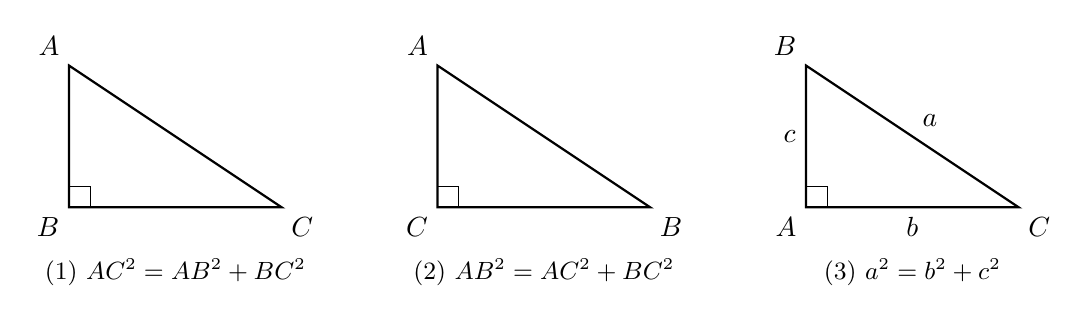
\begin{tikzpicture}[scale=0.9, >=latex]
  % (1) 角 B 為直角
  \begin{scope}[shift={(0,0)}]
    \coordinate (B) at (0,0);
    \coordinate (C) at (3,0);
    \coordinate (A) at (0,2);
    \draw[thick] (B) -- (C) -- (A) -- cycle;
    \draw (0,0.3) -- (0.3,0.3) -- (0.3,0);
    \node[below left] at (B) {$B$};
    \node[below right] at (C) {$C$};
    \node[above left] at (A) {$A$};
    \node[below=15pt] at (1.5,0) {\small (1) $AC^2 = AB^2 + BC^2$};
  \end{scope}

  % (2) 角 C 為直角
  \begin{scope}[shift={(5.2,0)}]
    \coordinate (C) at (0,0);
    \coordinate (B) at (3,0);
    \coordinate (A) at (0,2);
    \draw[thick] (C) -- (B) -- (A) -- cycle;
    \draw (0,0.3) -- (0.3,0.3) -- (0.3,0);
    \node[below left] at (C) {$C$};
    \node[below right] at (B) {$B$};
    \node[above left] at (A) {$A$};
    \node[below=15pt] at (1.5,0) {\small (2) $AB^2 = AC^2 + BC^2$};
  \end{scope}

  % (3) 角 A 為 90 度，邊長 a, b, c
  \begin{scope}[shift={(10.4,0)}]
    \coordinate (A) at (0,0);
    \coordinate (C) at (3,0);
    \coordinate (B) at (0,2);
    \draw[thick] (A) -- (C) node[midway, below] {$b$} -- (B) node[midway, above right] {$a$} -- cycle node[midway, left] {$c$};
    \draw (0,0.3) -- (0.3,0.3) -- (0.3,0);
    \node[below left] at (A) {$A$};
    \node[below right] at (C) {$C$};
    \node[above left] at (B) {$B$};
    \node[below=15pt] at (1.5,0) {\small (3) $a^2 = b^2 + c^2$};
  \end{scope}
\end{tikzpicture}
\caption{畢氏定理的幾種符號表示法對應圖}\label{fig:pythagoras_representations}
\end{figure}

上面三個表示法，都是正確的，並且顯然還有別的表示法。$\triangle$ 表示「三角形」，$A, B, C$ 表示三個平面上的點。$AC$ 表示「以 $A, C$ 為端點的一條線段」，並且顯然也表示了這條線段的長。這種區分在這裏並不是非常必要的，因為在這個問題裏，「線段」和「線段的長」並不需要確實區分。
\end{example}

在這門課中，我們還會遇到許多別的符號。大多數的符號，都會非常容易了解，但我們將在必要時，對所有的符號隨時加以說明。

\subsection*{習題 2-1}\label{sec:ex2-1}
\addcontentsline{toc}{subsection}{習題 2-1}

\begin{enumerate}[1., leftmargin=2em]
  \item 試以符號表示圓面積及圓周長之公式。
  \item 試以符號表示下面的敘述：\\
  「二相異正數之等差中項，必大於其等比中項。」
  \item 下面的一段文字中，有何不妥？請加以修改。\\
  「設 $a, b, c$ 為三線段的長，今以 $a, b, c$ 為三邊，作一三角形為 $\triangle ABC$。」
  \item 設有 $\triangle ABC$，試以符號表示下列各敘述：
  \begin{enumerate}[(i)]
    \item 它是直角三角形。
    \item 它是等腰三角形。
    \item 它是正三角形。
    \item 它是直角等腰三角形。
  \end{enumerate}
  \item 儘量以符號表示以下的定理（少用文字，多用符號）：
  \begin{enumerate}[(i)]
    \item 三角形中任意兩邊之和必大於第三邊。
    \item 三角形內角平分線交於一點，此點距此三角形之三邊等長。
  \end{enumerate}
  \item 令 $ABCD$ 為一個四邊形，試將下列各題中之符號用最簡明的文字敘述表示：
  \begin{enumerate}[(i)]
    \item $AB = CD$，$AD = BC$。
    \item $AB = CD$，$\angle DAC = 90^\circ$。
    \item $\angle A = \angle B = \angle C = \angle D = 90^\circ$。
    \item $AB = BC = CD = DA$，$\angle A = 90^\circ$。
    \item $\angle A = \angle B = \angle C = \angle D$，$AB = BC$。
    \item $AB = BC = CD = DA$。
    \item $\angle A + \angle C = 180^\circ$。
    \item $AB \parallel CD$。
  \end{enumerate}
  \item 試問下面的一段文字中，有何不妥？並作適當的修改。\\
  「設 $AB, CD$ 為二線段，將 $AB, CD$ 延長，令其交點為 $F$。」
  \item 試利用本節的方法，求 $879 + 654$ 之和，並解釋加法「逢十進位」的原理。同理，解釋 $782 + 978$ 和的「進位」原理。
  \item 觀察下列的平方數：
  \begin{align*}
    15^2 &= 225; & 25^2 &= 625; & 35^2 &= 1225; & 45^2 &= 2025; \\
    55^2 &= 3025; & 65^2 &= 4225; & 75^2 &= 5625; & 85^2 &= 7225; \\
    95^2 &= 9025; & 105^2 &= 11025; & \dots
  \end{align*}
  你能否發現到它們有一些共同規則嗎？（個位、十位的情形怎麼樣？百位以上的情形怎麼樣？）你能說明它們的理由嗎？\\
  〔提示：$(x+a)^2 = x^2 + 2ax + a^2$〕
  \item 推廣上題，考慮二數的乘積，如果這兩個數字的個位和為 $10$，十位以上之對應數字一一相同，像 $33 \times 37$，$42 \times 48$，$154 \times 156$，……那我們亦可得到類似上題之規則，請同學說明理由。\\
  〔提示：$(x+a)(x+b) = x^2 + (a+b)x + ab$〕
  \item[*] 觀察以下各數的平方：
  \begin{align*}
    11^2 &= 121; \\
    111^2 &= 12321; \\
    1111^2 &= 1234321; \dots \\
    (12345679 \times 9)^2 &= 12345678987654321.
  \end{align*}
  〔提示：$10 - 1 = 9$〕
\end{enumerate}

\subsection{集合}\label{sec:2-3}

\subsubsection*{甲、集合的概念}\label{subsec:2-3-a}

集合（set）是數學中很普遍的一個術語，一個集合是由它所含有的「元素」（element）（亦即組成單元）所湊集而成。譬如一條直線是由點所湊集成的集合，那些在這條直線上的點，就是該集合的元素。譬如在平面上，所有「和 $A$ 點的距離小於 $1$ 的點」成一集合，它所含的元素就是以 $A$ 點為圓心、$1$ 尺為半徑在平面上所畫的圓周以內的點（不包含圓周）。

\begin{figure}[htbp]
\centering
\begin{tikzpicture}[scale=1.1, >=latex]
  \draw[thick, dashed, fill=blue!10] (0,0) circle (1.5);
  \filldraw (0,0) circle (1.5pt) node[below] {$A$};
  \draw[->, thick] (0,0) -- (45:1.5) node[midway, above left] {$1$ 尺};
  \node at (0, 0.7) {\small 圓內部所有點組成的集合};
\end{tikzpicture}
\caption{平面上與 $A$ 點距離小於 $1$ 尺的點集示意}\label{fig:circle_interior_set}
\end{figure}

集合的概念是極簡單的，由一堆東西湊集而成的群體，就是一個集合。對於「一個集合」就數學的觀點而言，它只有一個要素：就是它所包含的那些「元素」。換句話說：\textbf{一個集合是由它所含有的元素完全決定！}（至於該集合各元素間是否具有相互關係？這些元素集成一個集合後是否有某種功效？從集合的觀念來說，是不相干的問題。）

在日常生活中，「集合」這個觀念是很普遍的。譬如某某學校的老師和同學們成一集合，你班上的同學們成一集合，你所在的教室中的桌椅成一集合，一隻錶的所有零件成一集合。但「集合的概念」只著重於其所含的「元素」，除此之外，沒有任何附帶涵義。一隻錶的零件，不論是將它們散放或者是將它們拼湊起來成為一隻能走的錶，由集合的觀點看來，都是同一集合，不加區分。

第一部集合論於公元 1878 年問世，由德國數學家康托（George Cantor, 1845--1918）所著。康托在書中解釋集合說：「集合是由明確而可鑑別的知覺對象或思維對象所聚合而成的，這些對象即稱為集合的元素。」

特別要請同學注意的是：\textbf{組成集合的元素必須明確可認定的}。譬如說：臺灣大學中文系漂亮的女生所成的集合，就很難確定。不說別的，李四覺得漂亮的，也許王二不以為然，在這情形下，達不成一致的規約，如何能定集合的元素呢？

\subsubsection*{乙、集合的描述}\label{subsec:2-3-b}

首先讓我們談一談集合的描述。

\begin{enumerate}[(一)]
  \item \textbf{列舉法}：假如一個集合 $A$ 只含有很少的幾個元素，則這個集合 $A$ 的一個最直截了當的表示法，就是把它所含的元素逐一列舉出來，通常我們再用括號 $\{\ \}$ 把列舉的元素括起來。
  
  \begin{example}\label{ex:2-3-1}
  \begin{enumerate}[(i)]
    \item $\{0, +1, -1\}$ 表示由 $0, +1, -1$ 三個元素所成的集合。
    \item $\{\triangle, \bigcirc, \square, \diamondsuit\}$ 表示由上述四個圖形所成的集合。
    \item $\{+, -, \times, \div\}$ 表示由 $+$, $-$, $\times$, $\div$ 四種運算符號所成的集合。
    \item $\{2, 3, 5, 7, 11, 13, 17, 19, 23, 29, 31, 37, 41, 43, 47, 53, 59, 61, 67, 71, 73, 79, 83, 89, 97\}$ 表示小於 $100$ 的二十五個正質數\footnote{\label{fn:prime}一個大於 $1$，而且除了 $1$ 和本身以外，不能被任何整數整除的數稱為「質數」，在第六章裏，我們將詳細討論它。}所成的集合。
  \end{enumerate}
  要注意的是：集合中括號內的元素可不顧順序，如
  \begin{align*}
    \{3, 7, 10\} &= \{10, 3, 7\} = \{7, 3, 10\}, \\
    \{\triangle, \bigcirc, \square, \diamondsuit\} &= \{\diamondsuit, \bigcirc, \square, \triangle\}.
  \end{align*}
  而且集合中同一元素書寫一次或多次，效果是一樣的，如
  \begin{align*}
    \{1, 2\} &= \{1, 2, 2, 2\}, \\
    \{2, 4, 6\} &= \{2, 2, 4, 6, 4, 6, 2\}, \\
    \{p, p, q, r\} &= \{p, q, r\}.
  \end{align*}
  \end{example}

  \item \textbf{特徵性質描述法}：從上面的最後一個例子，同學們可以看出當該集合的元素稍多一些的時候，逐一列舉的描述法是很煩瑣而不經濟的。另一種最常用的描述方法是：用該集合所含的元素的「特徵性質」去描述它。這種方法，我們以前已經用過，現在再舉例如下：
  
  \begin{example}\label{ex:2-3-2}
  \begin{enumerate}[(i)]
    \item 「偶數全體所成的集合」，「所有能被 $2$ 整除的整數所成的集合」，都是用來描述一個元素為 $0, \pm 2, \pm 4, \pm 6, \dots$ 的集合。
    \item 同樣地，「奇數全體所成的集合」，「所有不能被 $2$ 整除的整數所成的集合」，都是用來描述一個元素為 $\pm 1, \pm 3, \pm 5, \dots$ 的集合。
    \item 在平面 $P$ 上，一個以 $O$ 點為圓心、$1$ 尺為半徑的圓內的點所成的集合，也可以用「所有和 $O$ 點的距離小於 $1$ 尺的點所成的集合」去加以描述。
    \item $\{+\sqrt{2}, -\sqrt{2}\}$ 這一集合也可描述為「其平方為 $2$ 的數所成的集合」。
    \item 所有絕對值小於或等於 $1$ 的實數成一集合。
  \end{enumerate}
  \end{example}

  以上這種描述法是我們常用的。在本章第一節中我們曾一再強調數學符號的第一要素就是明確。所以在我們用「某一性質」去描述一個集合時，該性質一定要絕對明確；譬如：「大於 $100000$」是一個明確的性質，但是「相當大」就不是一個明確的性質。所以假如你隨隨便便說：「$A$ 是由相當大的有理數所成的集合」，別人一定會問究竟大到什麼程度才叫相當大？

  \item \textbf{典型元素描述法}：假如我們把列舉法與特徵性質法適當地加以配合，我們可以把集合所含的「典型元素」（typical element）加以描述。現在將例~\ref{ex:2-3-2} 中的五個例子，依次描述如下：
  \begin{enumerate}[(i)]
    \item $A = \{2n \mid n \text{ 為任意整數}\} = \{x \mid x \text{ 為整數，且能被 } 2 \text{ 整除}\}$。如以 $\mathbb{Z}$ 表示所有整數的集合，則又可寫成 $A = \{2n \mid n \in \mathbb{Z}\}$。
    \item $B = \{2n+1 \mid n \text{ 為任意整數}\} = \{x \mid x \text{ 為整數，且不能被 } 2 \text{ 整除}\} = \{2n+1 \mid n \in \mathbb{Z}\}$。
    \item $C = \{X \mid X \in P, OX \text{ 的長度} < 1 \text{ 尺}\}$。
    \item $D = \{x \mid x^2 = 2\}$。
    \item $E = \{x \mid |x| \le 1\}$。
  \end{enumerate}
  以上這種描述法在數學中是最常用的描述法，它和特徵性質描述法是很類似的。事實上，它就是把特徵性質描述法用適當的符號表示出來。
\end{enumerate}

\subsubsection*{丙、集合的記號}\label{subsec:2-3-c}

\begin{enumerate}[(一)]
  \item \textbf{屬於}：\\
  我們用符號「$\in$」表示「屬於」。式子
  \begin{equation}\label{eq:belong_rel}
    a \in B
  \end{equation}
  表示 $a$ 是集合 $B$ 的一個元素，讀做「$a$ 屬於 $B$」。譬如我們以 $A$ 表示所有絕對值大於 $1$ 的有理數所成的集合，則有：
  \begin{equation*}
    2 \in A, \quad -5 \in A, \quad \pm \frac{7}{2} \in A, \quad \frac{23}{3} \in A, \quad \dots \text{ 等等}。
  \end{equation*}
  相對地，我們用符號「$\notin$」表示「不屬於」。以上述集合 $A$ 為例，我們有：
  \begin{equation*}
    0 \notin A, \quad 1 \notin A, \quad -1 \notin A, \quad \frac{1}{2} \notin A, \quad -\frac{3}{5} \notin A, \quad \dots \text{ 等等}。
  \end{equation*}

  \item \textbf{子集}：\\
  假如集合 $A$ 的任一元素都一定也是集合 $B$ 的元素，我們就說 $A$ 是 $B$ 的一個「\textbf{子集}」。也可以說 $A$「包含於」$B$，或 $B$「包含」$A$，我們以符號
  \begin{equation}\label{eq:subset_rel}
    A \subseteq B \quad \text{或} \quad B \supseteq A
  \end{equation}
  表示之。要注意的是，按照上述定義，一個集合 $A$ 也是它本身的子集，亦即 $A \subseteq A$\footnote{\label{fn:subset_self}註：我們說明一下為什麼 $A \subseteq A$。讓我們看一看什麼叫做「$\subseteq$」：$A \subseteq B$ 的定義是：$A$ 中任一元素都一定是 $B$ 中某一元素。因此，$A \subseteq C$ 的定義是：$A$ 中任一元素都一定是 $C$ 中某一元素。因為上面的 $C$ 是可以變換的，假如我們把它變成 $A$，那麼 $A \subseteq A$ 的定義是：$A$ 中任一元素都一定也是 $A$ 中某一元素。這句話當然是對的（想一想：你班上的任一個同學，是不是你班上的某一個同學？）。因此，我們才可以說：由於「$\subseteq$」的定義，而且由於 $A$ 和 $A$ 之間滿足了這項定義，所以便有 $A \subseteq A$。有的書上把記號 $\subseteq$ 簡寫成 $\subset$，請同學在閱讀推演時先認清所用的符號。}。

  \begin{example}\label{ex:2-3-3}
  設：
  \begin{itemize}
    \item $A$ 是絕對值大於 $1$ 的有理數所成的集合，
    \item $B$ 是絕對值大於 $\frac{1}{3}$ 的有理數所成的集合，
    \item $C$ 是不等於 $0$ 的有理數所成的集合，
    \item $D$ 是大於 $1$ 的有理數所成的集合，
  \end{itemize}
  則上述四個集合間，有下述關係：
  \begin{equation*}
    A \subseteq B, \quad A \subseteq C, \quad B \subseteq C, \quad D \subseteq B, \quad D \subseteq C, \quad D \subseteq A,
  \end{equation*}
  且 $A \subseteq A, B \subseteq B, C \subseteq C, D \subseteq D$。
  \end{example}

  集合之間的關係，我們常以直觀而簡單的圖形表示。上面例子中 $A, B, C, D$ 四集合之間的關係，就可以用下面的圖形表示出來：

  \begin{figure}[htbp]
  \centering
  \begin{tikzpicture}[scale=0.9, >=latex]
    \draw[thick] (0,0) circle (3.2) node[below=2.6cm] {$C$（非零有理數）};
    \draw[thick] (0,0.3) circle (2.2) node[below=1.6cm] {$B$（$|x| > 1/3$）};
    \draw[thick] (0,0.6) circle (1.3) node[below=0.8cm] {$A$（$|x| > 1$）};
    \draw[thick] (0,1.1) circle (0.6) node {$D$（$x > 1$）};
  \end{tikzpicture}
  \caption{集合包含關係 $D \subseteq A \subseteq B \subseteq C$ 示意圖}\label{fig:nested_subsets}
  \end{figure}

  同學們不難從定義看出：「假如 $A$ 是 $B$ 的子集，$B$ 是 $C$ 的子集，則 $A$ 也是 $C$ 的子集。」亦即：
  \begin{equation}\label{eq:transitive_subset}
    \text{假如 } A \subseteq B, \ B \subseteq C, \text{ 則 } A \subseteq C,
  \end{equation}
  以圖表示如下：

  \begin{figure}[htbp]
  \centering
  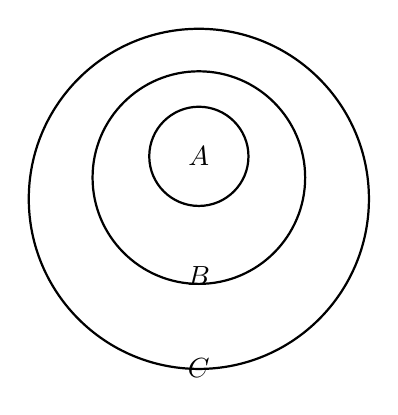
\begin{tikzpicture}[scale=0.9, >=latex]
    \draw[thick] (0,0) circle (2.4) node[below=1.9cm] {$C$};
    \draw[thick] (0,0.3) circle (1.5) node[below=1.0cm] {$B$};
    \draw[thick] (0,0.6) circle (0.7) node {$A$};
  \end{tikzpicture}
  \caption{子集關係的遞移性：$A \subseteq B$ 且 $B \subseteq C \implies A \subseteq C$}\label{fig:transitive_subset}
  \end{figure}

  \item \textbf{聯集與交集}：\\
  把集合 $A$ 的所有元素和集合 $B$ 的所有元素合併而成的集合叫做「\textbf{集合 $A, B$ 的聯集}」，以符號
  \begin{equation}\label{eq:union_def}
    A \cup B
  \end{equation}
  表示之。由一個集合 $A$ 和一個集合 $B$ 的公共元素所成的集合叫做「\textbf{集合 $A, B$ 的交集}」，以符號
  \begin{equation}\label{eq:intersection_def}
    A \cap B
  \end{equation}
  表示之。

  \begin{example}\label{ex:2-3-4}
  設 $A = \{1, 2\}$，$B = \{2, 3\}$，那麼：
  \begin{equation*}
    A \cup B = \{1, 2, 3\}, \qquad A \cap B = \{2\}。
  \end{equation*}
  \end{example}

  \begin{example}\label{ex:2-3-5}
  設 
  \begin{align*}
    A &= \{x \mid x \text{ 是實數，} -7 < x < 5\}, \\
    B &= \{x \mid x \text{ 是實數，} -3 < x < 10\},
  \end{align*}
  那麼
  \begin{align*}
    A \cup B &= \{x \mid x \text{ 是實數，} -7 < x < 10\}, \\
    A \cap B &= \{x \mid x \text{ 是實數，} -3 < x < 5\}。
  \end{align*}
  像 $A, B$ 這樣的集合，通常用符號
  \begin{equation*}
    A = (-7, 5), \qquad B = (-3, 10)
  \end{equation*}
  表示，稱為\textbf{開區間}。

  \begin{figure}[htbp]
  \centering
  \begin{tikzpicture}[scale=0.75, >=latex]
    \draw[->, thick] (-9, 0) -- (12, 0) node[right] {實數線};
    \foreach \x in {-8, -6, ..., 10} {
      \draw (\x, 0.15) -- (\x, -0.15) node[below] {\footnotesize \x};
    }
    % 區間 A: (-7, 5)
    \draw[thick, blue] (-7, 0.8) -- (5, 0.8);
    \draw[blue, fill=white] (-7, 0.8) circle (3pt);
    \draw[blue, fill=white] (5, 0.8) circle (3pt);
    \node[left, blue] at (-7, 0.8) {$A = (-7, 5)$};

    % 區間 B: (-3, 10)
    \draw[thick, red] (-3, 1.6) -- (10, 1.6);
    \draw[red, fill=white] (-3, 1.6) circle (3pt);
    \draw[red, fill=white] (10, 1.6) circle (3pt);
    \node[left, red] at (-3, 1.6) {$B = (-3, 10)$};

    % 交集 A cap B
    \draw[very thick, purple] (-3, 0) -- (5, 0);
    \draw[purple, fill=white] (-3, 0) circle (3pt);
    \draw[purple, fill=white] (5, 0) circle (3pt);
    \node[above, purple] at (1, 0.15) {\small $A \cap B = (-3, 5)$};
  \end{tikzpicture}
  \caption{開區間的聯集與交集在實數線上之圖解}\label{fig:open_intervals}
  \end{figure}
  \end{example}

  \begin{example}\label{ex:2-3-6}
  設 
  \begin{align*}
    C &= \{x \mid x \text{ 是實數，} -2 \le x \le 6\}, \\
    D &= \{x \mid x \text{ 是實數，} -4 \le x \le 3\},
  \end{align*}
  則
  \begin{align*}
    C \cup D &= \{x \mid x \text{ 是實數，} -4 \le x \le 6\} = [-4, 6], \\
    C \cap D &= \{x \mid x \text{ 是實數，} -2 \le x \le 3\} = [-2, 3]。
  \end{align*}
  如例~\ref{ex:2-3-5}，可用符號 $C = [-2, 6]$，$D = [-4, 3]$ 表示，稱為\textbf{閉區間}。一般來說，稱 $\{x \mid x \text{ 是實數，} a < x < b\}$ 為開區間，記為 $(a, b)$；而 $\{x \mid x \text{ 是實數，} a \le x \le b\}$ 稱為閉區間，記為 $[a, b]$。
  \end{example}

  \begin{example}\label{ex:2-3-7}
  設 $A$ 是下圖圓形中的點所成的集合，$B$ 是方形中的點所成的集合，則 $A \cup B$ 是左下圖中有斜線部分的點所成的集合，$A \cap B$ 是右下圖中有斜方格部分的點所成的集合。

  \begin{figure}[htbp]
  \centering
  \begin{minipage}[t]{0.45\textwidth}
  \centering
  \begin{tikzpicture}[scale=0.85]
    \fill[pattern=north east lines, pattern color=blue!60] (-0.8, 0) circle (1.3);
    \fill[pattern=north east lines, pattern color=blue!60] (0.2, -1.1) rectangle (2.2, 0.9);
    \draw[thick] (-0.8, 0) circle (1.3) node[left=18pt] {$A$};
    \draw[thick] (0.2, -1.1) rectangle (2.2, 0.9) node[right=18pt] {$B$};
    \node[below=15pt] at (0.6, -1.1) {\small 聯集 $A \cup B$（斜線部分）};
  \end{tikzpicture}
  \end{minipage}
  \hfill
  \begin{minipage}[t]{0.45\textwidth}
  \centering
  \begin{tikzpicture}[scale=0.85]
    \begin{scope}
      \clip (-0.8, 0) circle (1.3);
      \fill[pattern=grid, pattern color=red!70] (0.2, -1.1) rectangle (2.2, 0.9);
    \end{scope}
    \draw[thick] (-0.8, 0) circle (1.3) node[left=18pt] {$A$};
    \draw[thick] (0.2, -1.1) rectangle (2.2, 0.9) node[right=18pt] {$B$};
    \node[below=15pt] at (0.6, -1.1) {\small 交集 $A \cap B$（網格部分）};
  \end{tikzpicture}
  \end{minipage}
  \caption{幾何圖形點集的聯集與交集示意}\label{fig:geom_union_intersection}
  \end{figure}
  \end{example}

  從兩種集合 $A, B$ 得出它們的「聯集」與「交集」是很自然、很簡單的兩種運算。但是當 $A, B$ 兩集合不含任何公共元素時，如下圖所示：

  \begin{figure}[htbp]
  \centering
  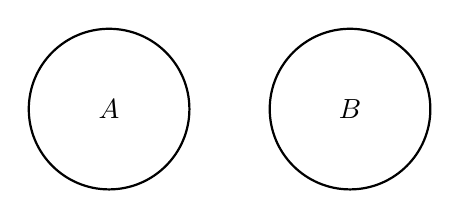
\begin{tikzpicture}[scale=0.85]
    \draw[thick] (-1.8, 0) circle (1.2) node {$A$};
    \draw[thick] (1.8, 0) circle (1.2) node {$B$};
  \end{tikzpicture}
  \caption{兩不相交集合示意}\label{fig:disjoint_sets}
  \end{figure}

  交集 $A \cap B$ 的意義是什麼呢？這裏我們只有兩種說法可供選擇：
  \begin{enumerate}[(i)]
    \item 我們可以在交集的定義中申明：當 $A, B$ 兩集合不含任何公共元素時，「$A, B$ 的交集」沒有意義，所以符號「$A \cap B$」也沒有意義。換句話說，$A \cap B$ 這個符號僅在 $A, B$ 有公共元素時，才能使用。
    \item 另外一種辦法是：引入一個特殊的「集合」，它不含任何元素，叫做「\textbf{空集合}」。然後說：當 $A, B$ 兩集合不含任何公共元素時，「$A, B$ 的交集」就是「空集合」。通常我們約定以符號「$\emptyset$」表示「空集合」，而上述事實用符號
    \begin{equation}\label{eq:disjoint_empty}
      A \cap B = \emptyset
    \end{equation}
    表示之。
  \end{enumerate}
  對於上述兩種辦法的取捨，自然得看哪一種辦法用起來較為方便簡明。經試用的結果，發現第二種辦法遠較第一種辦法簡潔易用，這也就是我們引入「空集合」這個特殊的集合的原因。

  \begin{example}\label{ex:2-3-8}
  奇數集合 $\cap$ 偶數集合 $= \emptyset$。
  \end{example}

  \begin{example}\label{ex:2-3-9}
  設 $A = \{x \mid x \text{ 為實數，} x > 0\}$，$B = \{x \mid x \text{ 為實數，} x < 0\}$，則 $A \cap B = \emptyset$。
  \end{example}
\end{enumerate}

\subsection*{習題 2-2}\label{sec:ex2-2}
\addcontentsline{toc}{subsection}{習題 2-2}

\begin{enumerate}[1., leftmargin=2em]
  \item 設 $\mathbb{N}$ 為所有自然數的集合，$\mathbb{Z}$ 為所有整數的集合，$\mathbb{Q}$ 為所有有理數的集合，$\mathbb{R}$ 為所有實數的集合，下列各數各屬於或不屬於哪些集合？用符號寫出。
  \begin{equation*}
    -3, \quad 0, \quad 1, \quad 2, \quad \frac{1+\sqrt{5}}{2}, \quad \frac{3}{7}, \quad -\frac{3}{4}, \quad 14。
  \end{equation*}
  \item 把下列各集合以第三種典型元素描述法寫出來，儘量運用符號：
  \begin{enumerate}[(i)]
    \item 平面 $P$ 上，以 $O$ 為圓心、$r$ 為半徑的圓周上的點。
    \item $A = \{1, 3, 5, 7, 9, 11, 13, 15, 17, 19\}$；$B = \{2, 4, 6, 8, 10, 12, 14, 16, 18, 20\}$；$C = \{7, 14, 21, 28, 35, 42\}$。
    \item 所有加上 $7$ 就大於 $15$ 的實數。
    \item 所有平方後就大於 $7$ 的實數。
  \end{enumerate}
  \item 設 $A$ 是所有平方數的集合，$B$ 是所有立方數的集合，將 $A, B$ 及 $A \cap B$ 以典型元素描述法寫出來。
  \item 下列集合中哪些是空集合？哪些只包含一個元素？
  \begin{align*}
    S_1 &= \{p \mid p \text{ 為質數，且 } 890 < p < 900\}, \\
    S_2 &= \{p \mid p \in \mathbb{N}, \ p \text{ 為可被 } 29 \text{ 整除的質數}\}, \\
    S_3 &= \{n \mid n \in \mathbb{N}, \text{ 且 } 3^n + 4^n = 5^n\}。
  \end{align*}
  \item 下列諸題中，判定 $A, B$ 二集合之關係：
  \begin{enumerate}[(i)]
    \item $A = \{x \mid 2x+4 \ge x-5\}$，$B = \{x \mid 3x+5 \ge 2x-4\}$。
    \item $A = \{x \mid x^2 + 4 = -2x+2\}$，$B = \{x \mid x^2 + 2x \le -2\}$。
    \item $A = \{x \mid a \le x \le b\}$，$B = \{y \mid 2a \le y \le 2b\}$，設 $a < 0 < b$。
    \item $A = \{x \mid x \text{ 為一等腰三角形}\}$，$B = \{y \mid y \text{ 為一等腰三角形}\}$。
    \item $A = \{a_i \mid i=1, 2, \dots, n\}$，$B = \{a_k \mid k=1, 2, 3, \dots, n+6\}$，$n \ge 1$。
    \item $A = \{x \mid x \text{ 是等腰三角形}\}$，$B = \{x \mid x \text{ 是正三角形}\}$。
  \end{enumerate}
  \item 把下列各集合寫成 $A \cap B$ 的型式，使 $A \nsubseteq B, B \nsubseteq A$，$A, B$ 都以典型方法表示：
  \begin{enumerate}[(i)]
    \item 所有大於 $3$ 小於 $5$ 的數。
    \item 所有正方形。〔提示：正方形為四邊等、四角相等的四邊形〕
    \item $12, 18$ 的最小公倍數的倍數。
    \item $\{P \mid OP = 5\}$（一切點都在一平面內）。
  \end{enumerate}
  \item 把下列各集合寫成 $A \cup B$ 之型式，且使 $A \nsubseteq B, B \nsubseteq A$：
  \begin{enumerate}[(i)]
    \item 所有不為 $3$ 除盡的整數。
    \item 所有的實數。
    \item 所有絕對值大於 $1$ 的實數。
  \end{enumerate}
  \item 設 $A$ 為所有四邊形的集合，$B$ 為所有梯形的集合，$C$ 為所有平行四邊形的集合，$D$ 為所有菱形的集合，$E$ 為所有長方形的集合，$F$ 為所有正方形的集合。以圖形表示下列各集合間之關係：
  \begin{enumerate}[(i)]
    \item $A, B, C, E, F$。
    \item $A, D, E, F$。
    \item $A, B, C, D, E, F$。
  \end{enumerate}
  \item 設 $A$ 為所有三角形的集合，$A_{90}$ 為所有直角三角形的集合，$B_2$ 為所有等腰三角形的集合，$B_3$ 為所有等邊三角形的集合，$A_{60}$ 為所有三角形中至少有一角為 $60^\circ$ 者所成的集合。
  \begin{enumerate}[(i)]
    \item 用圖形表示這些集合的關係。
    \item $A_{90} \cap B_3 = ?$
  \end{enumerate}
  \item 設 $A, B$ 表示二集合，試證：
  \begin{enumerate}[(i)]
    \item $A \subseteq A \cup B, \quad B \subseteq A \cup B$。
    \item $A \supseteq A \cap B, \quad B \supseteq A \cap B$。
    \item 設 $A \subseteq B$，而 $H$ 為任意集合，則 $A \cup H \subseteq B \cup H$。
    \item 設 $A \subseteq B$，而 $H$ 為任意集合，則 $A \cap H \subseteq B \cap H$。
    \item $A \cup (A \cap B) = A$。
    \item $B \cap (A \cup B) = B$。
  \end{enumerate}
  \item[*] 試證 $D = A \cap B$ 滿足下列兩性質：
  \begin{enumerate}[(1)]
    \item $D \subseteq A, \ D \subseteq B$。
    \item 滿足 $E \subseteq A, \ E \subseteq B$ 的任一集合 $E$，必定包含於 $D$。
  \end{enumerate}
  \item[*] 試證任一集合 $D$ 若滿足下列二性質：
  \begin{enumerate}[(1)]
    \item $D \subseteq A, \ D \subseteq B$。
    \item 滿足 $E \subseteq A, \ E \subseteq B$ 的任一集合 $E$，必定包含於 $D$。
  \end{enumerate}
  則此集合 $D$ 即為 $A \cap B$。
  \item[*] 試證 $C = A \cup B$ 滿足下二性質：
  \begin{enumerate}[(1)]
    \item $C \supseteq A, \ C \supseteq B$。
    \item 滿足 $F \supseteq A$ 且 $F \supseteq B$ 的任一集合 $F$，必定包含 $C$。
  \end{enumerate}
  \item[*] 試證任一集合 $C$ 若滿足下二性質：
  \begin{enumerate}[(1)]
    \item $C \supseteq A, \ C \supseteq B$。
    \item 滿足 $F \supseteq A$ 且 $F \supseteq B$ 的任一集合 $F$，必定包含 $C$。
  \end{enumerate}
  則此集合 $C$ 即為 $A \cup B$。
\end{enumerate}

\subsubsection*{丁、集合的差}\label{subsec:2-3-d}

對於集合 $A, B$，我們定義 $A, B$ 之間的「\textbf{差}」如下：
\begin{align*}
  A \setminus B &\text{ 是由所有「屬於 $A$ 但是不屬於 $B$」的元素所成的集合}； \\
  B \setminus A &\text{ 是由所有「屬於 $B$ 但是不屬於 $A$」的元素所成的集合}。
\end{align*}

\begin{figure}[htbp]
\centering
\begin{minipage}[t]{0.45\textwidth}
\centering
\begin{tikzpicture}[scale=0.85]
  \begin{scope}
    \clip (-0.8, 0) circle (1.3);
    \fill[pattern=north east lines, pattern color=blue!60] (-0.8, 0) circle (1.3);
  \end{scope}
  \fill[white] (0.2, -1.1) rectangle (2.2, 0.9);
  \draw[thick] (-0.8, 0) circle (1.3) node[left=18pt] {$A$};
  \draw[thick] (0.2, -1.1) rectangle (2.2, 0.9) node[right=18pt] {$B$};
  \node[below=15pt] at (0.6, -1.1) {\small 差集 $A \setminus B$};
\end{tikzpicture}
\end{minipage}
\hfill
\begin{minipage}[t]{0.45\textwidth}
\centering
\begin{tikzpicture}[scale=0.85]
  \begin{scope}
    \clip (0.2, -1.1) rectangle (2.2, 0.9);
    \fill[pattern=north west lines, pattern color=red!60] (0.2, -1.1) rectangle (2.2, 0.9);
  \end{scope}
  \fill[white] (-0.8, 0) circle (1.3);
  \draw[thick] (-0.8, 0) circle (1.3) node[left=18pt] {$A$};
  \draw[thick] (0.2, -1.1) rectangle (2.2, 0.9) node[right=18pt] {$B$};
  \node[below=15pt] at (0.6, -1.1) {\small 差集 $B \setminus A$};
\end{tikzpicture}
\end{minipage}
\caption{集合之差 $A \setminus B$ 與 $B \setminus A$ 示意}\label{fig:set_difference}
\end{figure}

\begin{example}\label{ex:2-3-10}
設 $A = \{1, 3, 5, 7\}$，$B = \{3, 7, 11\}$，$C = \{3, 9, 13\}$。則：
\begin{align*}
  A \setminus B &= \{1, 5\}, & A \setminus C &= \{1, 5, 7\}, \\
  B \setminus A &= \{11\}, & C \setminus A &= \{9, 13\}, \\
  B \setminus C &= \{7, 11\}, & C \setminus B &= \{9, 13\}。
\end{align*}
\end{example}

\begin{example}\label{ex:2-3-11}
設 $A = \text{直角三角形集合}$，$B = \text{等腰三角形集合}$。那麼 $A \setminus B$ 是「非等腰的直角三角形集合」，而 $B \setminus A$ 是「非直角的等腰三角形集合」。
\end{example}

\begin{example}\label{ex:2-3-12}
由一個實驗的結果造成的集合。

假如我們擲一個骰子兩次，而將它們可能的結果記錄下來，便有 $36$ 種可能的情形：
\begin{equation*}
\begin{array}{cccccc}
  (1, 1), & (1, 2), & (1, 3), & (1, 4), & (1, 5), & (1, 6), \\
  (2, 1), & (2, 2), & (2, 3), & (2, 4), & (2, 5), & (2, 6), \\
  \dots & & & & & \\
  (6, 1), & (6, 2), & (6, 3), & (6, 4), & (6, 5), & (6, 6)
\end{array}
\end{equation*}
〔$(3, 2)$ 表示第一次得 $3$，第二次得 $2$〕。令 $W$ 為以上 $36$ 種情形所成的集合，那麼許多「事件」便可以用子集表示出來。

例如：「第一次得 $5$」這一件「事」，便可由
\begin{equation*}
  A = \{(5, 1), (5, 2), (5, 3), (5, 4), (5, 5), (5, 6)\}
\end{equation*}
表示；而「兩次點數之和為 $7$」可以用
\begin{equation*}
  B = \{(1, 6), (2, 5), (3, 4), (4, 3), (5, 2), (6, 1)\}
\end{equation*}
表示。

而 $A \cap B$ 表示「第一次得 $5$ 而且兩次之和為 $7$」，我們可以看出，第二次的結果非 $2$ 不可，因此：
\begin{equation*}
  A \cap B = \{(5, 2)\}。
\end{equation*}
如果我們直接觀察 $A, B$ 兩個集合，發現 $(5, 2)$ 是它們唯一的共同元素，這樣也得到上面相同的結果。

此外我們還有：
\begin{itemize}
  \item $W \setminus A =$「第一次不得 $5$」；
  \item $W \setminus B =$「二次之和不得為 $7$」；
  \item $A \cup B =$「第一次得 $5$，或者兩次的和為 $7$」；
  \item $A \setminus B =$「第一次得 $5$，但第二次不得為 $2$」。
\end{itemize}
\end{example}

\subsubsection*{戊、集合運算法則}\label{subsec:2-3-e}

在上面一段中，我們引入下列有關集合的符號：
\begin{itemize}
  \item $\in$：屬於；如「$b \in A$」讀成「$b$ 屬於 $A$」。
  \item $\supseteq$：包含；如「$B \supseteq A$」讀成「$B$ 包含 $A$」。
  \item $\subseteq$：包含於；如「$A \subseteq B$」讀成「$A$ 包含於 $B$」。
  \item $\cap$：交集運算；如「$A \cap B$」讀成「$A, B$ 的交集」。
  \item $\emptyset$：空集合。
  \item $\cup$：聯集運算；如「$A \cup B$」讀成「$A, B$ 的聯集」。
  \item $\setminus$：差；如「$A \setminus B$」讀成「$A, B$ 之差」，「$B \setminus A$」讀成「$B, A$ 之差」。
\end{itemize}

注意：
\begin{enumerate}[(i)]
  \item 「$A, B$ 之差」和「$B, A$ 之差」是不同的兩個集合。
  \item 「$\in$」是元素和集合之間的關係，但是「$\supseteq$」和「$\subseteq$」是集合和集合之間的關係，後者有“比較”的意味在內。
\end{enumerate}

上述「運算」或「符號」之間具有很多有用的相互關連，現在說明如下：

\begin{enumerate}[(i)]
  \item 我們規定「空集合」$\emptyset$ 是任何集合的子集，亦即 $\emptyset \subseteq A$ 對任何集合 $A$ 皆成立。
  \begin{example}\label{ex:2-3-13}
  設集合 $A = \{1, 2, 3\}$，那麼 $A$ 的子集共有下列八個：
  \begin{equation*}
    \{1, 2, 3\}, \quad \{1, 2\}, \quad \{2, 3\}, \quad \{1, 3\}, \quad \{1\}, \quad \{2\}, \quad \{3\}, \quad \emptyset。
  \end{equation*}
  \end{example}

  \item 「$A \subseteq B$ 且 $B \subseteq A$」和「$A = B$」是一回事。
  \begin{example}\label{ex:2-3-14}
  設 $A$ 為所有三邊相等的三角形的集合，$B$ 為所有三個角相等的三角形的集合。當然，$A = B$。
  
  讓我們想一想為什麼 $A = B$：這是因為三邊相等的三角形，一定三個角也相等。亦即任一個 $A$ 中元素，也必都是 $B$ 中之元素，所以 $A \subseteq B$。反過來看，三個角都相等的三角形，一定也三邊相等。因此，任何 $B$ 中之元素，必也是 $A$ 中之元素，所以 $B \subseteq A$。有了這些了解，我們當然看出 $A$ 和 $B$ 非是同樣的集合不可，因為 $A$ 和 $B$ 中的元素都是「正三角形」，而一個集合又是完全被它所包含的元素決定的。
  
  一般說來，我們要證明二個集合 $A$ 和 $B$ 相等時，一個典型的方法就是先證明 $A \subseteq B$，再證明 $B \subseteq A$。這是因為由這裏可直接查核 $A, B$「是不是同一個集合」，而在另一面，「包含」的關係比較容易驗證。
  \end{example}

  \item 包含關係的多種等價描述：
  \begin{align*}
    \text{「} A \supseteq B \text{」和「} A \cap B = B \text{」是一回事}； \\
    \text{「} A \supseteq B \text{」和「} A \cup B = A \text{」也是一回事}； \\
    \text{「} A \supseteq B \text{」和「} B \setminus A = \emptyset \text{」也是一回事}。
  \end{align*}
  同學們請自行作圖驗證之。

  \item \textbf{交集運算的結合律}：
  \begin{equation}\label{eq:assoc_intersection}
    (A \cap B) \cap C = A \cap (B \cap C) = A \cap B \cap C,
  \end{equation}
  因為它們都是由 $A, B, C$ 的所有公共元素所成的集合。

  \item \textbf{聯集運算的結合律}：
  \begin{equation}\label{eq:assoc_union}
    (A \cup B) \cup C = A \cup (B \cup C) = A \cup B \cup C,
  \end{equation}
  因為它們都是把所有 $A, B, C$ 的元素合併而成的集合。

  \item \textbf{集合運算的分配律}：
  \begin{align}
    A \cap (B \cup C) &= (A \cap B) \cup (A \cap C), \label{eq:dist_cap_over_cup} \\
    A \cup (B \cap C) &= (A \cup B) \cap (A \cup C)。 \label{eq:dist_cup_over_cap}
  \end{align}

  \item \textbf{笛摩根定理}（De Morgan's Laws）：
  \begin{align}
    A \setminus (B \cup C) &= (A \setminus B) \cap (A \setminus C), \label{eq:demorgan_diff_cup} \\
    A \setminus (B \cap C) &= (A \setminus B) \cup (A \setminus C)。 \label{eq:demorgan_diff_cap}
  \end{align}
  上述 (vi), (vii) 兩點的理由我們留待下節再加說明，但是其大意可以從下圖清楚地看出：

  \begin{figure}[htbp]
  \centering
  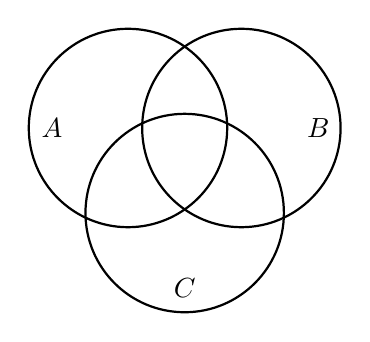
\begin{tikzpicture}[scale=0.9]
    \draw[thick] (-0.8, 0.5) circle (1.4) node[left=20pt] {$A$};
    \draw[thick] (0.8, 0.5) circle (1.4) node[right=20pt] {$B$};
    \draw[thick] (0, -0.7) circle (1.4) node[below=20pt] {$C$};
  \end{tikzpicture}
  \caption{三集合分配律與笛摩根定理文氏圖解析}\label{fig:venn_three_sets}
  \end{figure}

  請同學對上述三個集合 $A, B, C$ 逐一檢驗 (vi)、(vii) 中四個等式中所出現的每一集合，這對於上述等式的瞭解是很有幫助的。

  \begin{example}\label{ex:2-3-15}
  設 $A = \{1, 2, 3\}$，$B = \{2, 3, 4, 5\}$，$C = \{3, 5, 6\}$。
  \begin{itemize}
    \item 由於 $B \cup C = \{2, 3, 4, 5, 6\}$，$A \cap (B \cup C) = \{2, 3\}$。又 $A \cap B = \{2, 3\}$，$A \cap C = \{3\}$，$(A \cap B) \cup (A \cap C) = \{2, 3\}$。所以
    \begin{equation*}
      A \cap (B \cup C) = (A \cap B) \cup (A \cap C)。
    \end{equation*}
    \item 又因為 $B \cap C = \{3, 5\}$，$A \cup (B \cap C) = \{1, 2, 3, 5\}$。且 $A \cup B = \{1, 2, 3, 4, 5\}$，$A \cup C = \{1, 2, 3, 5, 6\}$，$(A \cup B) \cap (A \cup C) = \{1, 2, 3, 5\}$。所以
    \begin{equation*}
      A \cup (B \cap C) = (A \cup B) \cap (A \cup C)。
    \end{equation*}
  \end{itemize}
  \end{example}

  \begin{example}\label{ex:2-3-16}
  我們仍考慮例~\ref{ex:2-3-15} 中的 $A, B, C$：
  \begin{itemize}
    \item 因為 $A \setminus (B \cup C) = \{1\}$；又 $A \setminus B = \{1\}$，$A \setminus C = \{1, 2\}$，$(A \setminus B) \cap (A \setminus C) = \{1\}$。所以
    \begin{equation*}
      A \setminus (B \cup C) = (A \setminus B) \cap (A \setminus C)。
    \end{equation*}
    \item 又因為 $A \setminus (B \cap C) = \{1, 2\}$，且 $(A \setminus B) \cup (A \setminus C) = \{1, 2\}$。所以
    \begin{equation*}
      A \setminus (B \cap C) = (A \setminus B) \cup (A \setminus C)。
    \end{equation*}
  \end{itemize}
  \end{example}
\end{enumerate}

\subsubsection*{己、性質與集合的關係及元素個數計算}\label{subsec:2-3-f}

在上面我們提及可以用性質去描述一個集合，所以對於一個集合，我們也可以去討論它的元素所具有的共同性質。

譬如 $A$ 是所有具有性質 $\alpha$ 的元素所成的集合，$B$ 是所有具有性質 $\beta$ 的元素所成的集合，則：
\begin{itemize}
  \item $A \cap B$ 就是所有具有性質 $\alpha$ 和 $\beta$ 的元素所成的集合；
  \item $A \cup B$ 就是所有具有性質 $\alpha$ 或 $\beta$ 的元素所成的集合；
  \item $A \setminus B$ 是那些具有性質 $\alpha$，但是不具有性質 $\beta$ 的元素所成的集合。
\end{itemize}
集合和性質之間的關係也就是下一節所要討論的課題。

結束本節之前，讓我們舉例計算集合間聯集、交集與個數的關係。

\begin{example}\label{ex:2-3-17}
某大學新生註冊時規定學生課外活動必須就土風舞、橋藝、跆拳中至少任選一樣參加，註冊後統計獲得如下資料：有 $354$ 人參加土風舞社，有 $287$ 人參加橋藝社，$302$ 人參加跆拳社；其中又有 $54$ 人參加土風舞和橋藝，$85$ 人參加橋藝和跆拳，$77$ 人參加跆拳和土風舞，$35$ 人三樣都參加。試問此次新生註冊人數有多少？

\begin{figure}[htbp]
\centering
\begin{tikzpicture}[scale=1.0]
  \coordinate (A) at (-1.0, 0.7);
  \coordinate (B) at (1.0, 0.7);
  \coordinate (C) at (0, -0.8);

  \draw[thick] (A) circle (1.8);
  \draw[thick] (B) circle (1.8);
  \draw[thick] (C) circle (1.8);

  \node at (-2.3, 1.8) {$A$：土風舞社 ($354$ 人)};
  \node at (2.3, 1.8) {$B$：橋藝社 ($287$ 人)};
  \node at (0, -2.9) {$C$：跆拳社 ($302$ 人)};

  % 各分割區域人數標示
  \node at (0, 0.2) {$35$};
  \node at (0, 1.2) {$19$};
  \node at (-0.8, -0.2) {$42$};
  \node at (0.8, -0.2) {$50$};
  \node at (-1.6, 0.8) {$258$};
  \node at (1.6, 0.8) {$183$};
  \node at (0, -1.7) {$175$};
\end{tikzpicture}
\caption{三社團參加人數排容原理分割圖}\label{fig:pie_club_members}
\end{figure}

如果以 $n(A)$ 表示 $A$ 集合中元素的個數，則由圖形可看出：
\begin{align*}
  n(A \cap C) - n(A \cap B \cap C) &= 77 - 35 = 42 = n[(A \cap C) \setminus (A \cap B \cap C)], \\
  n(A \cap B) - n(A \cap B \cap C) &= 54 - 35 = 19 = n[(A \cap B) \setminus (A \cap B \cap C)], \\
  n(B \cap C) - n(A \cap B \cap C) &= 85 - 35 = 50 = n[(B \cap C) \setminus (A \cap B \cap C)], \\
  n(A) - 42 - 35 - 19 &= 258 = n[A \setminus (B \cup C)], \\
  n(B) - 19 - 35 - 50 &= 183 = n[B \setminus (C \cup A)], \\
  n(C) - 50 - 35 - 42 &= 175 = n[C \setminus (A \cup B)]。
\end{align*}
因此
\begin{align*}
  n(A \cup B \cup C) &= 175 + 42 + 35 + 50 + 19 + 258 + 183 \\
  &= 762。
\end{align*}
以後均以 $n(A)$ 表示集合 $A$ 中元素的個數。
\end{example}

\subsection*{習題 2-3}\label{sec:ex2-3}
\addcontentsline{toc}{subsection}{習題 2-3}

\begin{enumerate}[1., leftmargin=2em]
  \item 設 $\mathbb{N}$ 為所有自然數的集合，$\mathbb{Z}$ 為所有整數的集合，$A$ 為所有偶數的集合。
  \begin{enumerate}[(I)]
    \item 寫出它們之間的包含關係。
    \item 求 $\mathbb{N} \cap A$，$\mathbb{N} \setminus A$ 及 $A \setminus \mathbb{N}$。
  \end{enumerate}
  \item 設 $A$ 為所有大於 $2$ 的實數所成的集合，$B$ 為所有小於 $1$ 的實數所成的集合。求 $A \cup B, A \cap B, A \setminus B, B \setminus A$。
  \item 對於每一自然數 $n, n \ge 2$，令 $A_n$ 為 $n$ 的所有正質因數所成的集合，例如 $A_{30} = \{2, 3, 5\}$。試列出在下列情形中 $A_m$ 與 $A_n$ 之關係：
  \begin{enumerate}[(a)]
    \item $m$ 為 $n$ 的倍數。
    \item $m$ 與 $n$ 互質。
    \item $m$ 與 $n$ 的最大公因子 $k > 1$。
  \end{enumerate}
  \item 設 $I_k$ 為所有自然數 $k$ 的整數倍數，$k \ge 2$。試求 $I_k$ 與 $I_m$ 間的關係：
  \begin{enumerate}[(i)]
    \item $k$ 為 $m$ 的倍數。
    \item $k$ 與 $m$ 之最大公因子 $> 1$。
  \end{enumerate}
  \item 設 $A = \{x \mid x > 4\}$，$B = \{x \mid x \le 9\}$，$C = \{x \mid x \le 3\}$。按步找出 $A \setminus B$，$A \setminus C$ 及 $(A \setminus B) \cap (A \setminus C)$，再找出 $B \cup C$ 及 $A \setminus (B \cup C)$，由此驗證笛摩根定理。
  \item 設 $A, B$ 為二集合，$A$ 含有 $n_1$ 個元素，$B$ 含有 $n_2$ 個元素，$A \cap B$ 含有 $n_3$ 個元素。問 $A \setminus B$，$B \setminus A$ 與 $A \cup B$ 各含有多少元素？
  \item 老師出兩個習題給班上同學做，班上同學共有 $60$ 人，解出第一題的同學有 $37$ 人，解出第二題的同學有 $25$ 人，兩題都解出來的同學有 $8$ 人。問兩題都不會解的同學有幾人？
  \item 設集合 $A, B, C$ 各有 $n_1, n_2, n_3$ 個元素，$B \cap C, C \cap A, A \cap B$ 各有 $m_1, m_2, m_3$ 個元素，$A \cap B \cap C$ 有 $k$ 個元素。問 $A \cup B \cup C$ 含有多少元素？
  \item[*] 試證：
  \begin{enumerate}[(i)]
    \item $A \setminus (B \cup C) = (A \setminus B) \cap (A \setminus C)$。
    \item $A \setminus (B \cap C) = (A \setminus B) \cup (A \setminus C)$（即性質 vii）。
  \end{enumerate}
  \item 試證：
  \begin{equation*}
    \left.
    \begin{aligned}
      A \cup B &= A \cup C \\
      A \cap B &= A \cap C
    \end{aligned}
    \right\} \implies B = C。
  \end{equation*}
  \item 試判斷下列二式之正誤：
  \begin{enumerate}[(i)]
    \item $D \subseteq A \cap B \implies D \subseteq A$ 且 $D \subseteq B$。
    \item $D \subseteq A \cup B \implies D \subseteq A$ 或 $D \subseteq B$。
  \end{enumerate}
  在上二式中若發現錯誤，可舉出例子說明嗎？
  \item 若 $A \cup B = A \cap B$，試證 $A = B$。
\end{enumerate}

\subsection{簡易邏輯及基本數學語句}\label{sec:2-4}

在第一章中，我們概略地說明了「簡易邏輯」在數學中所扮演的角色。邏輯是用來討論「性質」與「性質」間的關係的工具，在這一節中，我們將利用「性質」與「集合」間的密切關係，簡潔地把今後要用到的簡易邏輯，為同學們交代清楚。

\subsubsection*{本節符號的用法}\label{subsec:2-4-notation}

在這一節中我們將用小寫希臘字母如 $\alpha, \beta, \gamma, \dots$ 等去表示「性質」，用相對的大寫英文字母如 $A, B, C, \dots$ 等去表示由滿足該性質的元素所成的集合，相對用的小寫英文字母如 $a, b, c, \dots$ 表示該集合的一個典型元素。

如果 $A$ 是由滿足性質 $\alpha$ 的元素所成的集合，我們簡述：$A$ 是由性質 $\alpha$ 所定的集合，而以
\begin{equation}\label{eq:prop_set_corresp}
  \alpha \longleftrightarrow A
\end{equation}
表示之。譬如 $\alpha$ 表示「是一個直角三角形」的性質，$A$ 是由滿足性質 $\alpha$ 所成的集合，這就是說 $A$ 是所有直角三角形的集合；$a \in A$ 是一個典型元素，這就是說 $a$ 是某一個直角三角形的意思。

\subsubsection*{甲、推演（deduction, implication）}\label{subsec:2-4-a}

「性質」和「性質」之間最重要的關係就是下面所要定義的推演關係：

設 $A$ 是由性質 $\alpha$ 所定的集合，$B$ 是由性質 $\beta$ 所定的集合。假如 $A$ 包含於 $B$（即 $A \subseteq B$），則由集合 $A, B$ 的定義可以知道性質 $\beta$ 是性質 $\alpha$ 的必然結論。換言之，任何一個具有性質 $\alpha$ 的元素 $a$（$a \in A$）必然也具有性質 $\beta$（因為 $A \subseteq B$）。上述關係我們用符號
\begin{equation}\label{eq:implication_def}
  \alpha \implies \beta
\end{equation}
表示之；讀做「$\alpha$ 推演得 $\beta$」（$\alpha$ implies $\beta$）。

所以，當 $\alpha \longleftrightarrow A$ 及 $\beta \longleftrightarrow B$ 時，
\begin{center}
  \textbf{「$\alpha \implies \beta$」和「$A \subseteq B$」是同一事實的兩種說法。}
\end{center}
從性質的觀點，我們說 $\alpha \implies \beta$（$\alpha$ 推演得 $\beta$）；從集合的觀點，我們說 $A \subseteq B$（$A$ 包含於 $B$）。

若 $\alpha \implies \beta$ 而且 $\beta \implies \alpha$，我們便以符號
\begin{equation}\label{eq:iff_def}
  \alpha \iff \beta
\end{equation}
表之。同樣的說法，我們在集合上已經用過：「$A \subseteq B$ 且 $B \subseteq A$」和「$A = B$」是一回事。因此，$\alpha \iff \beta$ 便相當於 $A = B$。

在日常的語言中，我們說：「某物具有性質 $\alpha$，則亦必具有性質 $\beta$」的意義，也就是上面所講的「$\alpha \implies \beta$」。

\begin{example}\label{ex:2-4-1}
設 $\alpha$ 表示「是一個 $4$ 的倍數」，$\beta$ 表示「是一個偶數」。則
\begin{equation*}
  A = \{4n \mid n \in \mathbb{Z}\}, \qquad B = \{2k \mid k \in \mathbb{Z}\}。
\end{equation*}
因為我們有 $\alpha \implies \beta$，同時我們也有 $A \subseteq B$。
\end{example}

\begin{example}\label{ex:2-4-2}
設 $\triangle ABC$ 為任一給定的三角形，設 $\alpha$ 表示「和 $\triangle ABC$ 全等」，$\beta$ 表示「和 $\triangle ABC$ 相似」，則
\begin{equation*}
  A = \{X \mid X \cong \triangle ABC\}, \qquad B = \{X \mid X \sim \triangle ABC\}。
\end{equation*}
因為兩全等三角形必然相似，所以 $\alpha \implies \beta$。同時，我們也可以看出 $A \subseteq B$。
\end{example}

\subsubsection*{乙、基本數學語句}\label{subsec:2-4-b}

幾個數學中常用的基本語句，我們將在下面統予明確的說明：

\begin{enumerate}[(i)]
  \item 「若 $\alpha$，則 $\beta$」與上述「$\alpha \implies \beta$」的意義完全一致。換言之，「若 $\alpha$，則 $\beta$」和「$\alpha$ 推演 $\beta$」只是同一事實的兩種說法。在這個時候，我們說：
  \begin{center}
    \textbf{$\alpha$ 是 $\beta$ 的充分條件，而 $\beta$ 是 $\alpha$ 的必要條件。}
  \end{center}
  \begin{example}\label{ex:2-4-3}
  如 $\alpha$ 表示「是一個等邊三角形」的性質，$\beta$ 表示「是一個等腰三角形」的性質。因為一個等邊三角形當然是等腰，所以 $\alpha \implies \beta$。此時「等邊」是「等腰」的充分條件，而「等腰」是「等邊」的必要條件。
  \end{example}

  \item 「$\alpha \iff \beta$」的意義是說性質 $\alpha$ 和性質 $\beta$ 是可互相推演得到的。這時我們說：
  \begin{center}
    \textbf{$\beta$ 是 $\alpha$ 的充分必要條件（充要條件），同時，$\alpha$ 也是 $\beta$ 的充分必要條件。}
  \end{center}
  \begin{example}\label{ex:2-4-4}
  如果 $\alpha$ 表示「是一個等腰三角形」的性質，$\beta$ 表示「是一個有兩角相等的三角形」的性質。幾何上我們可以證明 $\alpha \implies \beta$ 而且 $\beta \implies \alpha$，所以 $\alpha \iff \beta$。
  \end{example}

  \item （「和」字的用法）：「元素 $c$ 滿足 $\alpha$ 和 $\beta$」與「$c \in A \cap B$」同一意義。
  \begin{example}\label{ex:2-4-5}
  如果 $\alpha$ 表示「是一個偶數」的性質，而 $A$ 是所有偶數所成的集合；$\beta$ 表示「是 $3$ 的倍數」的性質，而 $B$ 是所有 $3$ 的倍數所成的集合。換句話說，$\alpha \longleftrightarrow A$，且 $\beta \longleftrightarrow B$。如果說 $c$ 滿足 $\alpha$ 和 $\beta$，就是說 $c$ 是一個偶數而且是 $3$ 的倍數，換句話說，$c \in A \cap B$（$A \cap B$ 是所有 $6$ 的倍數所成的集合）。
  \end{example}

  \item （「或」字的用法）：「元素 $c$ 滿足 $\alpha$ 或 $\beta$」與「$c \in A \cup B$」同一意義。
  \begin{example}\label{ex:2-4-6}
  如果 $\alpha$ 表示「大於 $5$ 的整數」的性質，$\beta$ 表示「小於 $7$ 的整數」的性質，而且 $\alpha \longleftrightarrow A$，$\beta \longleftrightarrow B$。$c$ 滿足 $\alpha$ 或 $\beta$，那麼 $c$ 至少要屬於 $A, B$ 中的一個。因為任何整數不論大於 $5$ 或小於 $7$，均至少滿足其一，所以 $A \cup B$ 就是所有的整數了。
  \end{example}
\end{enumerate}

\subsection*{習題 2-4}\label{sec:ex2-4}
\addcontentsline{toc}{subsection}{習題 2-4}

\begin{enumerate}[1., leftmargin=2em]
  \item 仿例~\ref{ex:2-4-2} 討論以下定理：
  \begin{enumerate}[(i)]
    \item 如 $\triangle ABC$ 為正三角形，則 $\triangle ABC$ 必為等腰三角形。
    \item 若 $\triangle ABC$ 中 $\angle C$ 為直角，則 $AB^2 = BC^2 + AC^2$。
  \end{enumerate}
  \item 下列各敘述 $\alpha \implies \beta$ 這種性質推演，請以典型元素集合表示法改寫為 $A \subseteq B$：
  \begin{enumerate}[(i)]
    \item 菱形必為平行四邊形。
    \item 正三角形必等腰。
    \item $16$ 的倍數必為 $4$ 的倍數。
    \item 一數可被 $a, b$ 除盡，則可被 $a, b$ 的最小公倍數除盡。
  \end{enumerate}
  \item 下列各敘述 $\alpha \iff \beta$ 這種性質的推演，請以典型元素法改寫為 $A = B$：
  \begin{enumerate}[(i)]
    \item $\triangle ABC$ 中，$\angle B = 90^\circ$ 的充分必要條件是 $AC^2 = AB^2 + BC^2$。
    \item $\triangle ABC$ 中，$AB = AC$ 的充分必要條件是 $\angle B = \angle C$。
    \item $x$ 是一個實數，$x < -3$ 或 $x > 3$ 的充要條件是 $x^2 > 9$。
  \end{enumerate}
  \item 對於下列各小題中 $A, B$，如果 $c \in A \cap B$，請寫出 $c$ 所滿足的性質：
  \begin{enumerate}[(i)]
    \item $A = \{x \mid x \text{ 是直角三角形}\}$，$B = \{x \mid x \text{ 是等腰三角形}\}$。
    \item $A = \{x \mid x > 3\}$，$B = \{x \mid x < 5\}$。
    \item $A = \{x \mid x \in \mathbb{R} \text{ 且 } x^2 - 6x + 8 < 0\}$，$B = \{x \mid x \in \mathbb{R} \text{ 且 } x^2 - 3x < 0\}$。
    \item $A = \{x \mid x \in \mathbb{R} \text{ 且 } ax^3 + bx^2 + cx + d = 0\}$，$B = \{x \mid x \in \mathbb{R} \text{ 且 } a'x + b' = 0\}$（只須以語言敘述）。
  \end{enumerate}
  \item 對於上列各小題中 $A, B$，如果 $c \in A \cup B$，請寫出 $c$ 所滿足的性質。
  \item 令 $\alpha$ 表示「是一個三角形」的性質，$\beta_2$ 表示「是一個等腰三角形」的性質，$\beta_3$ 表示「是一個等邊三角形」的性質，$\alpha_{60}$ 表示「是一個至少有一角為 $60^\circ$ 的三角形」的性質。試列出這些性質間的關係。
  \item 試以集合的觀點，判斷下列推論是否成立：\\
  「若 $x$ 為一實數，且 $x^2 < -1$，則 $x = 3$。」
  \item 設 $A$ 是 $B$ 的子集，$B$ 是 $C$ 的子集（即 $A \subseteq B, B \subseteq C$）。如 $a \notin A, b \notin B, c \notin C$，又 $d \in A, e \in B, f \in C$，則下列敘述何者正確？
  \begin{enumerate}[(i)]
    \item $a \notin C$
    \item $b \in A$
    \item $c \notin A$
    \item $d \in B$
    \item $e \in A$
    \item $f \in B$
  \end{enumerate}
  \item 試證：
  \begin{equation*}
    \left.
    \begin{aligned}
      A \cup B &= A \cup C \\
      A \cap B &= A \cap C
    \end{aligned}
    \right\} \implies B = C。
  \end{equation*}
  〔提示：先證「$A = B \iff (x \in A \iff x \in B)$」或「$A \subseteq B \iff (x \in A \implies x \in B)$」〕
\end{enumerate}

\subsubsection*{丙、基集（ground set）}\label{subsec:2-4-c}

對於一個給定問題的討論，往往很自然地存在一個「基礎集合」（簡稱\textbf{基集}），而該問題的討論中所涉及的集合都是那個基本集合的子集。

譬如我們在討論「平面幾何學」時所涉及的集合，如直線、圓、三角形等都是由平面上的某些點所成的集合，所以由全平面的點所成的集合就自然是「平面幾何學」的基集。同理，當我們討論「立體幾何學」時，那麼基集就自然地應該是「由全空間的點所成的集合」了！再者，假如我們在討論「有理數」的性質時，那麼「有理數全體所成的集合」對我們的討論而言，就是自然的基集；因為「實數全體所成的集合」包含「有理數全體所成的集合」，所以在討論「有理數」時，選取「實數全體所成的集合」為基集，也是可以的。

從上述例子，同學們可以看出下列幾點：
\begin{enumerate}[(i)]
  \item 「基集」隨著所要討論的問題而定。
  \item 對於一個給定的問題，「基集」的選取只要「夠廣」都可以。（不過一個自然的選取通常是最經濟的。）但是一旦選定後，在整個討論過程中是固定不變的。
\end{enumerate}
選定「基集」的一個主要目的是確立「補集」這一方便有用的概念。

\subsubsection*{丁、補集（complementary set）}\label{subsec:2-4-d}

設 $W$ 表示我們所選定的基集，所以本段中所涉及的集合 $A, B, C, D, \dots$ 都是 $W$ 的子集。

\begin{definition}[補集的定義]\label{def:complement}
$W \setminus A$ 叫做 $A$ 的\textbf{補集}，以符號「$\sim A$」表示之。
\end{definition}

\begin{example}\label{ex:2-4-7}
以平面幾何為例，取 $W = \text{平面的點所成的集合}$。設 $A$ 是下圖圓內及圓周上的點所成的集合，$B$ 是直線左邊的點所成的集合。

\begin{figure}[htbp]
\centering
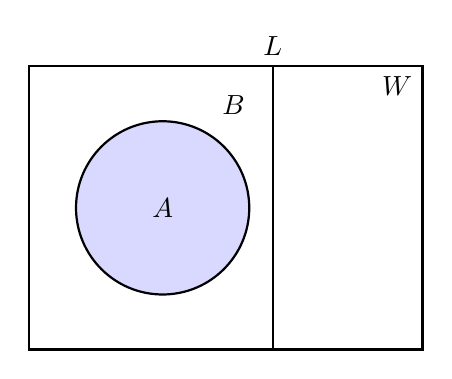
\begin{tikzpicture}[scale=1.0]
  \draw[thick] (-2.5, -1.8) rectangle (2.5, 1.8) node[below left] {$W$};
  \draw[thick, fill=blue!15] (-0.8, 0) circle (1.1) node {$A$};
  \draw[thick] (0.6, -1.8) -- (0.6, 1.8) node[above] {$L$};
  \node at (0.1, 1.3) {$B$};
\end{tikzpicture}
\caption{基集 $W$ 中的圓形點集 $A$ 與半平面點集 $B$ 補集示意}\label{fig:ground_set_complement}
\end{figure}

則 $\sim A$ 是圓外的點所成的集合，$\sim B$ 是直線右邊及直線上的點所成的集合。

請同學們自行找出 $\sim(A \cup B)$，$\sim(A \cap B)$，$(\sim A) \cap B$，$A \cap (\sim B)$，$(\sim A) \cup B$，$A \cup (\sim B)$，$(\sim A) \cap (\sim B)$，$(\sim A) \cup (\sim B)$，$\sim(A \cap (\sim B))$，$\sim(A \cup (\sim B))$ 等集合所表的區域，看看哪些是相同的集合。
\end{example}

假如 $A$ 是由性質 $\alpha$ 所定（亦即由性質 $\alpha$ 所描述），$B$ 是由性質 $\beta$ 所定，則：
\begin{itemize}
  \item $\sim A$ 是由那些不具有性質 $\alpha$ 的元素所成的集合；
  \item $\sim B$ 是由那些不具有性質 $\beta$ 的元素所成的集合。
\end{itemize}
我們將用符號「$\sim \alpha$」表示「$\alpha$ 的否定」（亦即不具有 $\alpha$）。

要注意：$\alpha$ 之否定，只有在基集 $W$ 確定時，才有意義。設 $\alpha$ 表示「是某校高一的男生」，假定基集 $W$ 為某校高一的所有學生的集合，那麼，$\sim \alpha$ 就表示「是高一的女生」。但是假如基集 $W$ 改為該校全體學生的集合，則 $\sim \alpha$ 便不止表示高一的女生，而其他各年級的男女生也都通通包含在內。

由集合運算法則：
\begin{align*}
  \sim(A \cap B) &= W \setminus (A \cap B) = (W \setminus A) \cup (W \setminus B) = (\sim A) \cup (\sim B), \\
  \sim(A \cup B) &= W \setminus (A \cup B) = (W \setminus A) \cap (W \setminus B) = (\sim A) \cap (\sim B)。
\end{align*}

\begin{example}\label{ex:2-4-8}
設 $W$ 為某校高中全體的學生的集合，$A$ 為該校高一的學生的集合，$B$ 為該校男生的集合。那麼，$A \cap B$ 為高一男生的集合，$\sim(A \cap B)$ 為所有「非」高一男生的集合，也就是該校女生的集合與高二、高三學生集合的聯集。同學們請對 $\sim(A \cap B) = (\sim A) \cup (\sim B)$ 作類似的解釋。
\end{example}

所以從上述對應可以看出：
\begin{enumerate}[(1)]
  \item $\sim(A \cap B) = (\sim A) \cup (\sim B) \iff \sim(\alpha \text{ 和 } \beta) \iff (\sim \alpha) \text{ 或 } (\sim \beta)$。\\
  亦即語句「$\alpha$ 和 $\beta$」的否定是「$(\sim \alpha)$ 或 $(\sim \beta)$」。
  \item $\sim(A \cup B) = (\sim A) \cap (\sim B) \iff \sim(\alpha \text{ 或 } \beta) \iff (\sim \alpha) \text{ 和 } (\sim \beta)$。\\
  亦即語句「$\alpha$ 或 $\beta$」的否定是「$(\sim \alpha)$ 和 $(\sim \beta)$」。
  \item 由 $\sim(\sim A) = A$，即得
  \begin{equation}\label{eq:double_negation}
    \sim(\sim \alpha) \iff \alpha
  \end{equation}
  （亦即否定的否定就是肯定）。
\end{enumerate}

為便於同學以後查考，將集合與性質（邏輯）之間的關係，列表如下：

\begin{table}[htbp]
\centering
\small
\renewcommand{\arraystretch}{1.3}
\begin{tabular}{|c|c|}
\hline
\textbf{集合語言} & \textbf{性質（邏輯）語言} \\ \hline
$A$ & $\alpha$ \\ \hline
$B$ & $\beta$ \\ \hline
$\sim A$ & $\sim \alpha$ \\ \hline
$\sim B$ & $\sim \beta$ \\ \hline
$A \cap B$ & $\alpha$ 和 $\beta$ \\ \hline
$A \cup B$ & $\alpha$ 或 $\beta$ \\ \hline
$A \subseteq B$ & $\alpha \implies \beta$ \\ \hline
$A = B$ & $\alpha \iff \beta$ \\ \hline
\end{tabular}
\caption{集合運算與邏輯語句對應表}\label{tab:set_logic_correspondence}
\end{table}

由此對應表，我們得到極重要之結論：
\begin{center}
  \textbf{「$A \subseteq B$」和「$\sim B \subseteq \sim A$」同義。} \\[0.3em]
  \textbf{「$\alpha \implies \beta$」和「$\sim \beta \implies \sim \alpha$」同義。}
\end{center}

\begin{example}\label{ex:2-4-9}
「等邊三角形一定是等腰三角形」與「不是等腰三角形一定不是等邊三角形」同義。

「$5$ 是比 $9$ 小的整數」但「比 $9$ 小的整數不一定是 $5$」。
\end{example}

\subsection*{習題 2-5}\label{sec:ex2-5}
\addcontentsline{toc}{subsection}{習題 2-5}

\begin{enumerate}[1., leftmargin=2em]
  \item 找出下列各補集來：
  \begin{enumerate}[(i)]
    \item $A$ 為正整數的集合，基集為所有整數的集合，$\sim A$ 是什麼？
    \item $A$ 為等腰三角形所成的集合，基集為所有三角形的集合，$\sim A$ 是什麼？
    \item $A$ 為正整數的集合，$B$ 為小於 $3$ 之整數的集合，基集為整數的集合，$\sim(A \cup B)$ 是什麼？$\sim(A \cap B)$ 是什麼？
    \item $A, B$ 與 (iii) 相同，基集為所有實數的集合，$\sim(A \cup B)$ 是什麼？
  \end{enumerate}
  \item 取實數的集合 $\mathbb{R}$ 為基集，並設 $A$ 為正數的集合，$B$ 為負數的集合，說明下列各集合：
  \begin{equation*}
    A \cap B, \quad (\sim A) \cap (\sim B), \quad (\sim A) \cup (\sim B), \quad (\sim A) \cup B, \quad A \cup (\sim B)。
  \end{equation*}
  \item 取 $W$ 為基集，試證：
  \begin{enumerate}[(i)]
    \item $\sim W = \emptyset$。
    \item $\sim \emptyset = W$。
    \item $A \cup (\sim A) = W$。
    \item $A \cap (\sim A) = \emptyset$。
  \end{enumerate}
  \item[*] 取自然數的集合 $\mathbb{N}$ 為基集，設 $\alpha$ 表示「是 $a$ 的倍數」的性質，$\beta$ 表示「是 $b$ 的倍數」的性質，假定 $\alpha \longleftrightarrow A$，$\beta \longleftrightarrow B$，請證明：
  \begin{enumerate}[(i)]
    \item $A \subseteq B \iff a \text{ 是 } b \text{ 的倍數}$。
    \item $A \cap B = \{x \mid x \text{ 是 } a, b \text{ 最小公倍數的倍數}\}$。
  \end{enumerate}
  \item 假定：(i)「$\alpha$ 或 $\beta \implies \gamma$」及 (ii)「$\alpha$ 或 $\sim \beta \implies \gamma$」均成立，試證「$\alpha \implies \gamma$」亦成立。（參照習題 2-3，第 10 題）
\end{enumerate}

\subsection*{附錄：羅馬數字乘法運算}\label{sec:ch2-appendix}
\addcontentsline{toc}{subsection}{附錄：羅馬數字乘法運算}

像 $365 \times 24 = 8760$ 這個乘式運算，若以羅馬數字符號表示，就成為以下複雜繁瑣的樣子：
\begin{align*}
  & (\mathrm{CCCLXV}) \cdot (\mathrm{XXIV}) \\
  &= (\mathrm{C}+\mathrm{C}+\mathrm{C}+\mathrm{L}+\mathrm{X}+\mathrm{V}) \cdot (\mathrm{X}+\mathrm{X}+\mathrm{V}-\mathrm{I}) \\
  &= \mathrm{C}\cdot\mathrm{X} + \mathrm{C}\cdot\mathrm{X} + \mathrm{C}\cdot\mathrm{X} + \mathrm{L}\cdot\mathrm{X} + \mathrm{X}\cdot\mathrm{X} + \mathrm{V}\cdot\mathrm{X} \\
  &\quad + \mathrm{C}\cdot\mathrm{X} + \mathrm{C}\cdot\mathrm{X} + \mathrm{C}\cdot\mathrm{X} + \mathrm{L}\cdot\mathrm{X} + \mathrm{X}\cdot\mathrm{X} + \mathrm{V}\cdot\mathrm{X} \\
  &\quad + \mathrm{C}\cdot\mathrm{V} + \mathrm{C}\cdot\mathrm{V} + \mathrm{C}\cdot\mathrm{V} + \mathrm{L}\cdot\mathrm{V} + \mathrm{X}\cdot\mathrm{V} + \mathrm{V}\cdot\mathrm{V} \\
  &\quad - \mathrm{C} - \mathrm{C} - \mathrm{C} - \mathrm{L} - \mathrm{X} - \mathrm{V} \\
  &= \mathrm{M}+\mathrm{M}+\mathrm{M}+\mathrm{D}+\mathrm{C}+\mathrm{L} + \mathrm{M}+\mathrm{M}+\mathrm{M}+\mathrm{D}+\mathrm{C}+\mathrm{L} \\
  &\quad + \mathrm{D}+\mathrm{D}+\mathrm{D}+\mathrm{C}+\mathrm{C}+\mathrm{L}+\mathrm{L}+\mathrm{X}+\mathrm{X}+\mathrm{V} - \mathrm{C} - \mathrm{C} - \mathrm{C} - \mathrm{L} - \mathrm{X} - \mathrm{V} \\
  &= \mathrm{M}+\mathrm{M}+\mathrm{M}+\mathrm{M}+\mathrm{M}+\mathrm{M}+\mathrm{M}+\mathrm{C}+\mathrm{C}+\mathrm{C}+\mathrm{M}+\mathrm{D}+\mathrm{C}+\mathrm{C}+\mathrm{C}+\mathrm{X}+\mathrm{X}+\mathrm{V} \\
  &\quad - \mathrm{C} - \mathrm{C} - \mathrm{C} - \mathrm{L} + \mathrm{X} - \mathrm{V} \\
  &= \mathrm{M}+\mathrm{M}+\mathrm{M}+\mathrm{M}+\mathrm{M}+\mathrm{M}+\mathrm{M}+\mathrm{M}+\mathrm{D}+\mathrm{C}+\mathrm{C}+\mathrm{C} - \mathrm{L} + \mathrm{X} \\
  &= \mathrm{M}+\mathrm{M}+\mathrm{M}+\mathrm{M}+\mathrm{M}+\mathrm{M}+\mathrm{M}+\mathrm{M}+\mathrm{D}+\mathrm{C}+\mathrm{C}+\mathrm{L}+\mathrm{X} \\
  &= \mathrm{MMMMMMMMDCCLX} \quad (= 8760)。
\end{align*}
 % 第二章 符號用法、基本數學語句及集合的概念
% =========================================================================
% 《高中數學實驗教材》第一冊（高一上） 
% 第三章 數的概念
% =========================================================================

\section{數的概念}\label{sec:ch3}

「自然數系」、「有理數系」和「實數系」，這些「數」是由種種自然界所常見的「量」，歸納其共同性質而得的體系。它們是有效討論各種關於量的問題所不可或缺的工具。上述諸數系的基本性質是數學的基礎與根源所在。本章將詳述數的源起，自然數及有理數的基本性質。由於實數系的一部份性質較為深些，而且在目前並不需要用它，故實數系的基本性質，將留待第二冊才為同學們作一有系統的介紹。

\subsection{\S 3-1\quad 數的源起}\label{sec:3-1}

在第一章的甲段討論數學的題材時，我們已簡略地談到數的源起。對於具有天然個別單元的量，我們只需要「數一數」它們有多少「個」，而自然數也就是用以「計數」個數的工具。同學們都已熟習自然數的加與乘這兩種基本運算，在下一節中我們將詳述自然數系對於加與乘這兩種基本運算所具有的基本性質。現在讓我們簡要地談談加與乘這兩種運算的源起：

\subsubsection*{甲、「+1」運算與加法、乘法}\label{subsec:plus_one}

「$1$」是自然的起點，
\begin{equation}\label{eq:count_start}
  2 = 1+1, \quad 3 = 2+1, \quad 4 = 3+1, \quad 5 = 4+1, \quad \dots, \quad 97 = 96+1, \quad \dots
\end{equation}
所以「$+1$」（加一）是自然中最原始的運算。

事實上，我們所知道的加法與乘法，通通可以看做是「$+1$」這個運算的推廣，下面我們繼續說明這件事。

假如我們把「$+1$」這種運算做兩遍，如 $(5+1)+1 = 5+2$，或 $(6+1)+1 = 6+2$ 等，這就是「$+2$」的意思\footnote{\label{fn:plus_two}「$(a+1)+1$」這個符號，就是表示把「$a$」這個數，用「$+1$」連做兩遍的意思。小括弧 $(a+1)$ 表示做第一次「$+1$」；做完之後，再「$+1$」一次，豈不是剛好做了兩遍？因此，適當地利用符號，可以將一些要用文字才能說清楚的事，說得更明白。}，亦即「$+2$」的意思是 $((a+1)+1)$。以此類推，「$+3$」就是把「$+1$」重複做三遍，「$+4$」就是把「$+1$」重複做四遍……等等，亦即
\begin{align}
  a+3 &= ((a+1)+1)+1 \label{eq:add_three}\\
  a+4 &= (((a+1)+1)+1)+1 \label{eq:add_four}
\end{align}
所以「$a+b$」就是對 $a$ 作 $b$ 次「$+1$」運算的縮寫。

其次讓我們看一看乘法的運算：
\begin{align*}
  a &= 1 \times a \\
  a+a &= 2 \times a \\
  a+a+a &= 3 \times a \\
  a+a+a+a &= 4 \times a
\end{align*}
由上面諸式，不難看出 $b \times a$ 也就是 $b$ 個 $a$ 相加的縮寫。

\subsubsection*{乙、度量與數系的擴張}\label{subsec:measure_expansion}

在第一章的甲段中，我們也談到另一類不具有「天然單元」的量，如「長度」、「質量」、「體積」等，並以長度為例，討論了如何去度量這一類的量。簡單的說，度量的方法是先取一個人為的單位，然後去求「所要度量的量」和「所取定的單位」間的比值，這種比值是一個「實數」。換言之，「實數系」也是度量的工具。從對長度的度量的討論中，有
\begin{equation}\label{eq:number_systems_hierarchy}
  \text{實數系} \supset \text{有理數系} \supset \text{自然數系}
\end{equation}
這一重要的相互關係。我們將循序漸進，先去瞭解「自然數系」的性質，然後經由「自然數系」和「有理數系」間的相互關係去瞭解「有理數系」的性質。在第二冊中，我們將再進一步經由「有理數系」和「實數系」間的相互關係去瞭解「實數系」的性質。

\begin{figure}[htbp]
\centering
\begin{tikzpicture}[scale=1.0, >=latex]
  % 數系包含層級示意圖
  \draw[thick, fill=blue!8] (0, 0) ellipse (4.5cm and 2.4cm);
  \draw[thick, fill=blue!18] (-0.3, -0.2) ellipse (3.2cm and 1.7cm);
  \draw[thick, fill=blue!30] (-0.6, -0.4) ellipse (1.8cm and 1.0cm);

  \node at (-0.6, -0.4) {\textbf{自然數系} $\mathbb{N}$};
  \node[above] at (-0.3, 0.5) {\textbf{有理數系} $\mathbb{Q}$};
  \node[above] at (0, 1.4) {\textbf{實數系} $\mathbb{R}$};
  
  \node[font=\footnotesize, text=gray!80!black] at (2.4, -0.8) {無理數（如 $\sqrt{2}, \pi$）};
  \node[font=\footnotesize, text=gray!80!black] at (1.2, 0.4) {負分數、非整數分數};
  \node[font=\footnotesize, text=gray!80!black] at (-0.6, -1.0) {$1, 2, 3, \dots$};
\end{tikzpicture}
\caption{數系的層次包含關係示意圖}\label{fig:number_hierarchy}
\end{figure}

\subsection{\S 3-2\quad 自然數系的基本性質}\label{sec:3-2}

「數」是討論種種「關於量的問題」的有效工具，但是我們必須先切實瞭解這些「工具」的基本特性才能真正發揮其效用。自然數系是上述「數」中最簡單也是最基本的，所以自然數系的基本性質是整個體系的重要基礎！同學們切不可因為「它們看起來簡單平凡」而忽略它，要知道世間有用的道理就是那些簡單而不凡的道理，要點在於：能心領神會、能活用這些簡單而不凡的道理！

\subsubsection*{甲、本節符號的用法}\label{subsec:nat_notation}

我們將用 $\mathbb{N}$ 表示所有自然數所成的集合，即
\begin{equation}\label{eq:set_N}
  \mathbb{N} = \{1, 2, 3, 4, \dots, n, \dots\}
\end{equation}
我們將用小寫字母 $a, b, c, \dots$ 等來表示 $\mathbb{N}$ 中的任何一個元素。於是，我們就可以用這樣的符號，很方便地去討論，去描述自然數系的「通性」。譬如：
\begin{equation}\label{eq:sum_not_one}
  a+b \neq 1 \qquad (\forall\, a, b \in \mathbb{N})
\end{equation}
表示任何兩個自然數的和絕不等於 $1$。換言之，上述一個式子充分地表達了所有下述式子的全體：（注意：零「$0$」不屬於 $\mathbb{N}$。）
\begin{align*}
  1+1 \neq 1, \quad 1+2 \neq 1, \quad 1+3 \neq 1, \quad 1+4 \neq 1, \quad \dots \\
  2+1 \neq 1, \quad 2+2 \neq 1, \quad 2+3 \neq 1, \quad 2+4 \neq 1, \quad \dots \\
  3+1 \neq 1, \quad 3+2 \neq 1, \quad 3+3 \neq 1, \quad 3+4 \neq 1, \quad \dots \\
  4+1 \neq 1, \quad 4+2 \neq 1, \quad 4+3 \neq 1, \quad 4+4 \neq 1, \quad \dots
\end{align*}
同理，下述諸式：
\begin{align*}
  1+1=1+1, \quad 1+2=2+1, \quad 1+3=3+1, \quad 1+4=4+1, \quad 1+5=5+1, \quad \dots \\
  2+2=2+2, \quad 2+3=3+2, \quad 2+4=4+2, \quad 2+5=5+2, \quad \dots \\
  3+3=3+3, \quad 3+4=4+3, \quad 3+5=5+3, \quad \dots
\end{align*}
就可以簡潔地用 $a+b = b+a$ 總括地加以表達。

\subsubsection*{乙、自然數系基本性質}\label{subsec:nat_axioms}

列述自然數系的基本性質如下：
\begin{enumerate}[I.]
  \item 任何一自然數，均可由 $1$ 開始，經有限次「$+1$」運算而得。換句話說，由 $1$ 開始，逐次「$+1$」，即可得到任一自然數，這就叫做「\textbf{數學歸納法（mathematical induction）原理}」。
  \item $(a+b)+c = a+(b+c)$。（加法結合律）
  \item $a+b = b+a$。（加法交換律）
  \item $a+b = c+b \iff a = c$。（$\Rightarrow$ 的部分叫做加法對消律）
  \item $(a+b) \cdot c = a \cdot c + b \cdot c$。（分配律）
  \item $a \cdot b = b \cdot a$。（乘法交換律）
  \item $(a \cdot b) \cdot c = a \cdot (b \cdot c)$。（乘法結合律）
  \item $a \cdot b = c \cdot b \iff a = c$。（$\Rightarrow$ 的部分叫做乘法對消律，注意：零「$0$」不是自然數，所以 $b \neq 0$。）
\end{enumerate}

同學們對於自然數的次序都已十分清楚，現在我們來仔細看看甚麼叫做 $3 < 5$。我們知道 $3 < 5$，是因為 $5$ 在自然數中排在 $3$ 的後面，即由 $3$ 出發，經兩次「$+1$」運算就得到 $5$（即 $5 = 3 + 2$）。一般地：

\begin{definition}[自然數的大小次序]\label{def:nat_order}
設 $a, b \in \mathbb{N}$。若存在一個自然數 $u \in \mathbb{N}$，使得
\begin{equation}\label{eq:nat_greater}
  a = b + u
\end{equation}
我們就說「$a$ 大於 $b$」，記作 $a > b$；或說「$b$ 小於 $a$」，記作 $b < a$。
\end{definition}

由次序的定義，當 $a > b$ 時，我們可以逐次從 $a$ 中減去 $b$（即以 $b$ 除 $a$），直到剩下的數小於 $b$ 為止。這就是同學們在小學學過的整數除法：對任意給定之 $a, b \in \mathbb{N}$，存在商數 $q$ 與餘數 $r$，使得 $a = bq + r$。若餘數 $r = 0$，則稱 $b$ 整除 $a$。

\subsection*{習題 3-1}\label{sec:ex3-1}
\addcontentsline{toc}{subsection}{習題 3-1}

\begin{enumerate}[1., leftmargin=2em]
  \item 求下列各組數相除的商數與餘數：
  \begin{enumerate}[(i)]
    \item $a = 732, \quad b = 24$。
    \item $a = 365, \quad b = 7$。
    \item $a = 719415, \quad b = 365$。
    \item $a = 30, \quad b = 7$。
    \item $a = 1973, \quad b = 54$。
  \end{enumerate}
  \item 一數 $x$ 除以 $7$，餘 $3$；一數 $y$ 除以 $7$，餘 $2$；那麼 $xy$ 除以 $7$ 的餘數是多少呢？
  \item 一數 $x$ 除以 $9$，餘 $4$；一數 $y$ 除以 $9$，餘 $5$；求 $xy$ 除以 $9$ 的餘數。
\end{enumerate}

\subsubsection*{丙、數學歸納法}\label{subsec:induction}

我們現在來略為討論一下數學歸納法，數學歸納法是自然數的性質 I 的另一種表示方法，有用處的地方很多，我們今後也會常常用到。現在我們舉例說明如下：

\begin{example}\label{ex:sum_integers}
求證對所有自然數 $n$，
\begin{equation}\label{eq:sum_n}
  1+2+3+\dots+n = \frac{n(n+1)}{2} \qquad \dots\dots (1)
\end{equation}
\end{example}

\begin{proof}
當 $n=1$ 時，我們有
\begin{equation*}
  1 = \frac{1(1+1)}{2}
\end{equation*}
因此 (1) 式是對的，我們也不難看出在 $n=2, 3, 4$ 時 (1) 式都滿足，但是，我們怎樣才知道 (1) 式是對所有的自然數都對呢？

我們想一想，甚麼叫「所有的自然數」，又，我們怎樣才能得到「所有的自然數」？根據性質 I，所有的自然數可以自 $1$ 開始，一次一次地由「$+1$」而得到，因此，我們來看一看怎樣利用這個性質來證明 (1)。

在 $n=k$ 時，(1) 成為
\begin{equation}\label{eq:ind_hyp}
  1+2+\dots+k = \frac{k(k+1)}{2} \qquad \dots\dots (2)
\end{equation}
在 $n=k+1$ 時，(1) 的左邊應該是
\begin{equation}\label{eq:ind_lhs}
  1+2+\dots+k+(k+1) \qquad \dots\dots (3)
\end{equation}
右邊應該是
\begin{equation}\label{eq:ind_rhs}
  \frac{(k+1)(k+2)}{2} \qquad \dots\dots (4)
\end{equation}
（我們還不知道 (2) 是否成立，也不知道 (3) 是否等於 (4)）但是假如我們：
\begin{align*}
  &\text{從 } n=1 \text{ 證到 } n=2 (=1+1) \\
  &\text{從 } n=2 \text{ 證到 } n=3 (=2+1) \\
  &\text{從 } n=3 \text{ 證到 } n=4 (=3+1) \\
  &\dots\dots \\
  &\text{從 } n=k \text{ 證到 } n=k+1 \qquad \dots\dots (5)
\end{align*}
那麼，我們豈不是對「所有的自然數」都證明了 (1)？請注意在這裏 $k$ 是一個典型的自然數。因此，如果我們證明了 (2) $\implies$ (3)=(4)，那麼便等於證明了 (5) 的全體。所以，若是要對所有的自然數證明 (1) 式，我們只要再證明 (2) $\implies$ (3)=(4) 就夠了，這就是數學歸納法的精神。

根據歸納假設 (2)：
\begin{align*}
  (3) &= 1 + 2 + \dots + k + (k+1) \\
  &= (1 + 2 + \dots + k) + (k+1) \\
  &= \frac{k(k+1)}{2} + (k+1) \\
  &= (k+1)\left(\frac{k}{2} + 1\right) \\
  &= (k+1)\left(\frac{k+2}{2}\right) \\
  &= \frac{(k+1)(k+2)}{2} = (4)
\end{align*}
因此，我們用數學歸納法證明了 (1)。
\end{proof}

有些不等式也可以用數學歸納法證明，讓我們舉一個例子來說明：

\begin{example}[伯努利不等式]\label{ex:bernoulli}
設 $p > 0$，求證 $(1+p)^n \ge 1+np$，式中 $n$ 為自然數。
\end{example}

\begin{proof}
當 $n=1$ 時，上式的左右兩邊都是 $1+p$。所以不等式成立，而實際上這時可以改成等號。

設 $n=k$ 時不等式成立，即 $(1+p)^k \ge 1+kp$。當 $n=k+1$ 時，
\begin{align*}
  (1+p)^{k+1} &= (1+p)^k (1+p) \ge (1+kp)(1+p) \\
  &= 1 + kp + p + kp^2 = 1 + (k+1)p + kp^2
\end{align*}
因為 $k \in \mathbb{N}$ 且 $p > 0$，故 $kp^2 > 0$。因此 $1 + (k+1)p + kp^2 > 1 + (k+1)p$，得
\begin{equation*}
  (1+p)^{k+1} \ge 1 + (k+1)p
\end{equation*}
由數學歸納法原理知，不等式對所有自然數 $n$ 均成立。
\end{proof}

\begin{example}\label{ex:collinear_fallacy}
在運用數學歸納法時，必須特別注意推論的邏輯嚴謹性與起步條件。例如有人提出下列命題：「平面上任意給定的 $n$ 個點必共線。」並給出偽證明：當 $n=1, 2$ 時顯然任兩點在一直線上；假定 $n=k$ 時任 $k$ 點共線，則取 $k+1$ 點時，前 $k$ 點共線，後 $k$ 點亦共線，從而推論 $k+1$ 點共線。這個錯誤在於兩組點集的交集必須至少有兩點才能確定同一直線，故在由 $k=2$ 推至 $k=3$ 時即已失效。正確的幾何命題應敘述為：「若平面上任意三點皆在一直線上，則任意 $n$ 點必在同一直線上。」
\end{example}

\subsection*{習題 3-2}\label{sec:ex3-2}
\addcontentsline{toc}{subsection}{習題 3-2}

\begin{enumerate}[1., leftmargin=2em]
  \item 有人用下法證明全世界的人性別都一樣。設一集合 $M_n$ 包含 $n$ 個人，則想證明 $M_n$ 中的人性別都一樣。當 $n=1$ 時，$M_1$ 中只有一個人，當然其性別是唯一的。現在假定命題 $n=k$ 時成立；再假定 $M_{k+1}$ 是包含 $k+1$ 個人的集合，在 $M_{k+1}$ 中選定兩個人 $x$ 和 $y$，則 $M_{k+1} \setminus \{x\}$ 和 $M_{k+1} \setminus \{y\}$ 都是只包含 $k$ 個人的集合，所以其中的人性別都一樣，因而 $x, y$ 和 $M_{k+1} \setminus \{x, y\}$ 中任何人的性別都相同，故 $M_{k+1}$ 中諸位的性別必全相同。請指正這證明錯在哪裡？
  \item 等差級數求和的公式也可以用數學歸納法證明，你能做出嗎？
  \item 對任意 $n \in \mathbb{N}$，試說明 $n^2 - n + 41$ 不恆為質數（請找出反例）。
  \item 試用數學歸納法證明下式：
  \begin{equation*}
    1^2 + 2^2 + 3^2 + \dots + n^2 = \frac{n(n+1)(2n+1)}{6}
  \end{equation*}
  \item 設 $n$ 為正整數，試證：
  \begin{equation*}
    (1^5 + 2^5 + 3^5 + \dots + n^5) + (1^7 + 2^7 + 3^7 + \dots + n^7) = 2 \left[\frac{n(n+1)}{2}\right]^4
  \end{equation*}
  \item 試證：
  \begin{equation*}
    1^3 + 2^3 + 3^3 + \dots + n^3 = (1+2+3+\dots+n)^2 = \left[\frac{n(n+1)}{2}\right]^2
  \end{equation*}
  \item 設 $n$ 是正整數，試證：
  \begin{equation*}
    1 + 3 + 5 + \dots + (2n-1) = n^2
  \end{equation*}
  \item 試證：
  \begin{equation*}
    1 \cdot 2 \cdot 3 + 2 \cdot 3 \cdot 4 + \dots + n(n+1)(n+2) = \frac{n(n+1)(n+2)(n+3)}{4}
  \end{equation*}
\end{enumerate}

\subsubsection*{丁、基本性質的推論}\label{subsec:nat_corollaries}

利用上述「自然數系」的基本性質 I--VIII，我們可以推演得所有「自然數系」的重要性質，而且以後我們逐步討論整數系，有理數系及實數系等數系的基本性質時，上述自然數系的基本性質 I--VIII 就是我們的起點。

我們現在列舉幾個基本性質的簡單推論：

\begin{prop}[次序推論 XI]\label{prop:nat_xi}
設 $a, b, c \in \mathbb{N}$：
\begin{enumerate}[(1)]
  \item $a > b \iff a+c > b+c$。
  \item $a = b \iff a+c = b+c$。
  \item $a < b \iff a+c < b+c$。
\end{enumerate}
\end{prop}

\begin{proof}
$a > b \iff$ 存在 $u \in \mathbb{N}$，使得 $a = b + u$（「$>$」的定義）。
\begin{align*}
  &\iff a+c = (b+u)+c \\
  &\iff a+c = b+(u+c) && \text{〔性質 II 加法結合律〕} \\
  &\iff a+c = b+(c+u) && \text{〔性質 III 加法交換律〕} \\
  &\iff a+c = (b+c)+u && \text{〔性質 II 加法結合律〕} \\
  &\iff a+c > b+c && \text{〔「$>$」的定義〕}
\end{align*}
同理可知 $a < b \iff a+c < b+c$。
\end{proof}

\begin{remark}
往後證明或運算時，當然不必如上面這樣細項，譬如從 $a+c = (b+u)+c$ 我們可以把上述三步合成一步，導得 $a+c = (b+c)+u$。
\end{remark}

\begin{prop}[次序推論 XII]\label{prop:nat_xii}
設 $a, b, c \in \mathbb{N}$（注意：$c \in \mathbb{N}$，所以 $c$ 是正的！）：
\begin{enumerate}[(1)]
  \item $a > b \iff a \cdot c > b \cdot c$。
  \item $a = b \iff a \cdot c = b \cdot c$。
  \item $a < b \iff a \cdot c < b \cdot c$。
\end{enumerate}
\end{prop}

\begin{proof}
我們現在先證明 (1)：
\begin{align*}
  a > b &\implies \text{存在 } u \in \mathbb{N} \text{ 使得 } a = b + u && \text{〔「$>$」之定義〕} \\
  &\implies a \cdot c = (b + u) \cdot c = bc + uc && \text{〔性質 V 分配律〕}
\end{align*}
因 $u \in \mathbb{N}, c \in \mathbb{N} \implies uc \in \mathbb{N}$，由「$>$」之定義，得 $ac > bc$。

反之，若 $ac > bc$，我們想證明 $a > b$。因 $a > b, a = b, a < b$ 只有一種、必有一種會成立（三一律），所以我們先看 $a < b$ 會不會成立。假如 $a < b$，則 $b > a$，而由上面的證明可知 $bc > ac$，亦即 $ac < bc$，但是我們假定 $ac > bc$，所以 $a < b$ 不會成立。

再看 $a = b$ 會不會成立呢？由性質 VIII 可知 $a = b \implies ac = bc$，又和我們的假定 $ac > bc$ 矛盾，因此 $a = b$ 也不會成立。因此只有 $a > b$ 會成立，至此我們證明了 (1)。

在 (1) 的敘述中將 $a, b$ 互換，便得到 $b > a \iff bc > ac$，亦即 $a < b \iff ac < bc$。
\end{proof}

\begin{remark}
上面最後所用的證明方法，叫做\textbf{窮舉法}（排除法）。當問題的本身有相當的對稱性時，適當地利用這些對稱性有時可以省去很多不必要的麻煩。
\end{remark}

\begin{prop}[次序遞移律 X]\label{prop:nat_x}
設 $a, b, c \in \mathbb{N}$。如果 $a > b$ 並且 $b > c$，則 $a > c$。
\end{prop}

\begin{proof}
$a > b$ 且 $b > c \implies$ 存在 $u \in \mathbb{N}$ 使 $a = b+u$，且存在 $v \in \mathbb{N}$ 使 $b = c+v$。
\begin{align*}
  a &= b + u = (c + v) + u \\
  &= c + (v + u) && \text{〔性質 II〕} \\
  &\implies a > c && \text{〔因 $v+u \in \mathbb{N}$〕}
\end{align*}
故得證。
\end{proof}

\begin{prop}[同向不等式相加與相乘]\label{prop:nat_ineq_add_mul}
設 $a, b, c, d \in \mathbb{N}$：
\begin{itemize}
  \item[\textup{(XI')}] 如果 $a > b$ 並且 $c > d$，則 $a+c > b+d$。
  \item[\textup{(XII')}] 如果 $a > b$ 並且 $c > d$，則 $a \cdot c > b \cdot d$。
\end{itemize}
\end{prop}

\begin{example}\label{ex:power_order}
對於任何自然數 $a, b, n$，如果 $a > b$，那麼 $a^n > b^n$。
\end{example}

\begin{proof}
我們利用數學歸納法來證明：當 $n=1$ 時，$a^1 > b^1$ 顯然成立。設 $n=k$ 時 $a^k > b^k$ 成立，由於性質 XII' 和 $a > b$ 的性質，我們有
\begin{equation*}
  a^{k+1} = a^k \cdot a > b^k \cdot b = b^{k+1}
\end{equation*}
所以對於任何自然數 $n$，這個式子都成立。
\end{proof}

\subsection*{習題 3-3}\label{sec:ex3-3}
\addcontentsline{toc}{subsection}{習題 3-3}

\begin{enumerate}[1., leftmargin=2em]
  \item 試證明上面的性質 (XI') 及 (XII')。
  \item 試證 $2^{10n} > 3^{2n}$，$n$ 為自然數。
  \item 試證 $2^{3n} < 10^n$，$n$ 為自然數。
  \item 利用 $5^2 = 3^2 + 4^2$，證明 $5^n > 3^n + 4^n$（$n > 2$）。
  \item 當 $n \ge 4$ 時，證明 $3^n > n^3$。〔提示：$(n+1)^3 = n^3 + 3n^2 + 3n + 1$〕
\end{enumerate}

\subsubsection*{戊、數系性質的初步應用}\label{subsec:nat_app}

學到這裏，許多同學可能會有些「吃悶葫蘆」的感覺，因為我們一直在吹這些如分配律、交換律、結合律、對消律……等數的基本性質多麼要緊，多麼有用，但是它們的要緊性，它們的用處到底在什麼地方呢？我們在這裏先講一個小故事，初步說明一下它們的廣泛應用。

\begin{example}[等差級數求和]\label{ex:gauss_arith}
據說當年大數學家高斯（C. F. Gauss, 1777--1855）在六、七歲時就是老愛發問，有一次老師給他下面的題目，叫他好好去算，希望他能夠安靜一會兒，題目是：
\begin{equation*}
  1+2+3+4+5+\dots+96+97+98+99+100 = ?
\end{equation*}
殊不知不到一、兩分鐘，高斯小朋友就迅速而準確地把上面一百個數目加好了，他的算法如下：
\begin{align*}
  S &= 1 + 2 + 3 + \dots + 98 + 99 + 100 \\
  +) \quad S &= 100 + 99 + 98 + \dots + 3 + 2 + 1 \\
  \hline
  2S &= 101 + 101 + 101 + \dots + 101 + 101 + 101 \quad (\text{共 } 100 \text{ 個}) \\
  &= 100 \times 101 = 10100
\end{align*}
所以
\begin{equation*}
  S = \frac{1}{2} \times 100 \times 101 = 5050
\end{equation*}
他的老師對他這麼小小年紀，即能靈活運用數的性質去解決問題，大為賞識器重。
\end{example}

上述算法也就是「等差級數」的求和法。下列級數叫做「等差級數」：
\begin{equation}\label{eq:arith_series}
  a + (a+d) + (a+2d) + \dots + (a+(n-1)d)
\end{equation}
$a$ 叫做它的首項，$d$ 叫做它的公差，$n$ 是它的項數，令 $S$ 為其總和，則由下式：
\begin{align*}
  S &= a + (a+d) + (a+2d) + \dots + [a+(n-1)d] \\
  +) \quad S &= [a+(n-1)d] + [a+(n-2)d] + \dots + (a+d) + a \\
  \hline
  2S &= [2a+(n-1)d] + [2a+(n-1)d] + \dots + [2a+(n-1)d] \quad (\text{共 } n \text{ 個}) \\
  &= n[2a+(n-1)d]
\end{align*}
故
\begin{equation}\label{eq:arith_sum_formula}
  S = \frac{n[2a+(n-1)d]}{2} = \frac{n(\text{首項} + \text{末項})}{2}
\end{equation}

講到等差級數可以順便提一下「等比級數」：
\begin{equation}\label{eq:geom_series}
  a + ar + ar^2 + \dots + ar^{n-1}
\end{equation}
其中 $a$ 稱為首項，$r$ 稱為公比，$n$ 是項數，令 $S$ 為其總和，則由下式：
\begin{align*}
  S &= a + ar + ar^2 + \dots + ar^{n-1} \\
  -) \quad rS &= \phantom{a +} ar + ar^2 + \dots + ar^{n-1} + ar^n \\
  \hline
  S - rS &= a - ar^n
\end{align*}
即 $S(1-r) = a(1-r^n)$。當 $r \neq 1$ 時，可得：
\begin{equation}\label{eq:geom_sum_formula}
  S = \frac{a(1-r^n)}{1-r}
\end{equation}

以上求法有它巧妙整齊的技巧，與等差級數求和的方法類似，但我們亦可以從另一角度來看這問題，這就是下一例題所要用的遞迴證法。

\begin{example}\label{ex:powers_of_two_sum}
求證 $1+2+4+8+\dots+2^{n-1} = 2^n - 1$。
\end{example}

\begin{proof}
我們只要證明：
\begin{equation}\label{eq:two_pow_recur}
  1 + (1+2+4+\dots+2^{n-1}) = 2^n \qquad \dots\dots (1)
\end{equation}
就夠了。(1) 式的左邊為：
\begin{align*}
  &= 1 + 1 + 2 + 2^2 + 2^3 + \dots + 2^{n-1} \\
  &= (1+1) + 2 + 2^2 + 2^3 + \dots + 2^{n-1} \\
  &= 2 + 2 + 2^2 + 2^3 + \dots + 2^{n-1} \\
  &= (2+2) + 2^2 + 2^3 + \dots + 2^{n-1} = 2^2 + 2^2 + 2^3 + \dots + 2^{n-1} \\
  &= 2^3 + 2^3 + \dots + 2^{n-1} \\
  &= \dots\dots \\
  &= 2^{n-1} + 2^{n-1} = 2 \cdot 2^{n-1} = 2^n
\end{align*}
故得證。
\end{proof}

用例~\ref{ex:powers_of_two_sum} 的聚項求和法可以推廣到等比級數求和公式，推廣的步驟留作習題。

以上的例子，有一個有趣的解釋。假如你跟別人賭博，第一次下注 $1$ 元，如果輸了，便下注 $2$ 元；如果再輸了，便下注 $2^2 = 4$ 元；再輸了便下注 $2^3 = 8$ 元……直到你贏一次為止。假如你一直輸了 $n$ 次，而在第 $n+1$ 次才贏，那麼你贏回的錢是 $2^n$，而前 $n$ 次輸掉的總錢數是 $1+2+4+\dots+2^{n-1} = 2^n - 1$。因此淨賺：
\begin{equation*}
  2^n - (1+2+4+\dots+2^{n-1}) = 2^n - (2^n - 1) = 1 \text{ 元}
\end{equation*}
因此，看起來似乎是：「假如你不停地賭下去，每次賭注加倍，只要贏一次，那麼，你一定會贏一塊錢。」

這也許就是為什麼許多賭徒傾家蕩產的理由！進一步的理由，等到高三機率的時候，可以清楚地向各位同學說明。在這裏，我們只提醒一句：在我們想到「贏一塊錢」的時候，我們還要同時考慮「贏一塊錢的機會與代價」。在另一方面，我們也要提醒大家，在 $n$ 並不很大時，這個數目 $2^n$ 會變得非常大：

\begin{table}[htbp]
\centering
\small
\renewcommand{\arraystretch}{1.2}
\begin{tabular}{|c|r|r|}
\hline
\textbf{連輸次數 $n$} & \textbf{第 $n$ 次下注額} & \textbf{連輸 $n$ 次後輸的總數} \\ \hline
1  & $1 = 2^0$      & $1$ \\ \hline
2  & $2 = 2^1$      & $1+2 = 3$ \\ \hline
3  & $4 = 2^2$      & $1+2+4 = 7$ \\ \hline
4  & $8 = 2^3$      & $1+2+4+8 = 15$ \\ \hline
5  & $16 = 2^4$     & $31$ \\ \hline
6  & $32 = 2^5$     & $63$ \\ \hline
7  & $64 = 2^6$     & $127$ \\ \hline
8  & $128 = 2^7$    & $255$ \\ \hline
9  & $256 = 2^8$    & $511$ \\ \hline
10 & $512 = 2^9$    & $1023$ \\ \hline
11 & $1024 = 2^{10}$ & $2047$ \\ \hline
12 & $2048 = 2^{11}$ & $4095$ \\ \hline
13 & $4096 = 2^{12}$ & $8191$ \\ \hline
14 & $8192 = 2^{13}$ & $16383$ \\ \hline
15 & $16384 = 2^{14}$ & $32767$ \\ \hline
16 & $32768 = 2^{15}$ & $65535$ \\ \hline
\end{tabular}
\caption{加倍下注賭博模型的指數增長表}\label{tab:gambler_ruin}
\end{table}

因此，假如你連輸 $15$ 次，你便輸掉 $32767$ 元，而你若在第 $16$ 次下注 $32768$ 元才贏，也不過是把輸掉的補平之後，只淨贏得一元！

\subsection*{習題 3-4}\label{sec:ex3-4}
\addcontentsline{toc}{subsection}{習題 3-4}

\begin{enumerate}[1., leftmargin=2em]
  \item 試求 $1+3+5+7+\dots+99$ 的和。
  \item 仿例~\ref{ex:powers_of_two_sum} 求 $2 + 2 \cdot 3 + 2 \cdot 3^2 + 2 \cdot 3^3 + \dots + 2 \cdot 3^n$ 的和；由此再求出 $1 + 3 + 3^2 + 3^3 + \dots + 3^n$ 的和。
  \item 例~\ref{ex:powers_of_two_sum} 和第 2 題，可以推廣到下面求和公式：
  \begin{equation*}
    1 + x + x^2 + \dots + x^n = \frac{1 - x^{n+1}}{1 - x} \qquad (x \neq 1)
  \end{equation*}
  \item 有一個 6 位數，若將最左邊的數字移到最右邊，則得一新六位數，若此新數為原數的 3 倍，問原來的 6 位數是什麼？
  \item 考慮一個大數字如：$37656289705$，我們知道，因為 $3+7+6+5+6+2+8+9+7+0+5 = 58$，$5+8=13$，$1+3=4$；此數不可能被 9 整除（甚至不可能被 3 整除），這便是有名的「棄九法」，請問棄九法的道理在哪裏？我們也知道最後所得的 4，恰巧是原數除以 9 所得的餘數，請問這又是何道理？
  \item 設一四位數字 $Z = \overline{z_3 z_2 z_1 z_0}$，其中 $z_3, z_2, z_1, z_0$ 表示 $Z$ 中各位數字，今令 $D = (z_0 + z_2) - (z_1 + z_3)$，試證 $Z - D$ 可被 11 整除。
  \item 有一自然數 $x$ 可以化成 10 進位的展式，那麼此展式是唯一的，也就是說如果：
  \begin{align*}
    x &= a_n \cdot 10^n + a_{n-1} \cdot 10^{n-1} + \dots + a_1 \cdot 10 + a_0 \\
    &= b_n \cdot 10^n + b_{n-1} \cdot 10^{n-1} + \dots + b_1 \cdot 10 + b_0
  \end{align*}
  則 $a_0 = b_0, a_1 = b_1, a_2 = b_2, \dots, a_n = b_n$。其中 $a_i, b_i$ 為 0 到 9 的整數之一。
  \item 試求下列各式前 $n$ 項的和：
  \begin{enumerate}[(i)]
    \item $9 + 99 + 999 + \dots$
    \item $3 + 33 + 333 + \dots$
    \item $1 + 11 + 111 + \dots$
    \item $7 + 77 + 777 + \dots$
  \end{enumerate}
\end{enumerate}

\subsection{\S 3-3\quad 整數系}\label{sec:3-3}

自然數系對於「加、乘」這兩種基本代數運算雖然具備了交換律、結合律、分配律、對消律等優良性質，但是在許多代數問題的討論中，每當我們遇到下列簡單方程式如：
\begin{enumerate}[(i)]
  \item $a+x=b$，求解 $x=?$
  \item $b \cdot x = a$（$b \neq 0$），求解 $x=?$
\end{enumerate}
就不一定能在自然數系中求得出解。譬如 (i) 式：當 $a=3, b=5$ 時有解 $x=2$；但是當 $a=5, b=3$ 時就無解。一般說來，當 $a \ge b$ 時，(i) 式在自然數系中是無解的\footnote{註：在正整數系中「沒有解」的意思是對任何正整數 $x$，$a+x=b$ 亦即 $5+x=3$ 都不可能成立。（因為若 $x$ 為正整數，則 $5+x > 5 > 3$，所以 $5+x$ 永遠不會等於 $3$）。因此我們知道 $5+x=3$ 在正整數系中沒有解。}。又如 (ii) 式，當 $b=3, a=5$ 時無解，但當 $b=3, a=6$ 時有解 $x=2$。所以對於許多需要解 (i)、(ii) 兩種型式的代數問題來說，自然數系很不夠用，我們要在本節中討論補救辦法。

\subsubsection*{甲、整數的產生}\label{subsec:int_generation}

把自然數系加上「$0$」，即 $\mathbb{N} \cup \{0\}$，就得非負整數集 $\mathbb{Z}^+$，這樣當 $a=b$ 時，(i) 式就有解 $x=0$，滿足 $a+0=a$。

對任一 $a \in \mathbb{N}$，把一個能使 $a+x=0$ 的數 $x$ 記作 $x = -a$，讀成「負 $a$」，即：
\begin{align*}
  \text{當 } a = 1, \quad &\text{有 } x = -1 \\
  \text{當 } a = 2, \quad &\text{有 } x = -2 \\
  \text{當 } a = 3, \quad &\text{有 } x = -3
\end{align*}
這樣得到的量 $x$，統稱為\textbf{負整數}，以符號 $\mathbb{Z}^-$ 記之。在正整數加上 $0$ 與所有負整數，就可以做成\textbf{整數集}：
\begin{equation}\label{eq:integers_set}
  \mathbb{Z} = \{\dots, -3, -2, -1, 0, 1, 2, 3, \dots\}
\end{equation}
我們有 $\mathbb{Z} \supset \mathbb{N}$。

這樣當 $a > b$ 時，(i) 式 $a+x=b$ 在 $\mathbb{Z}$ 中就有解 $x = -(a-b)$ 了，其中 $a-b$ 為正整數，故 $x = -(a-b)$ 為負整數；通常記為 $x = b - a$。

\subsubsection*{乙、整數的次序}\label{subsec:int_order}

在自然數系中，我們可以比較任意兩個自然數的大小。如果有一個 $u \in \mathbb{N}$ 使得 $a+u=b$，那麼我們知道在自然數次序的排列中 $a$ 排在 $b$ 的前面，也就是說 $a < b$。因為整數可以自然地排成：
\begin{equation*}
  \dots, -3, -2, -1, 0, 1, 2, 3, \dots
\end{equation*}
所以我們也可規定：如果兩個整數在上面排列中，$a$ 在 $b$ 的前面，則稱做 $a < b$。這種說法的精神和自然數中的說法一樣，因此我們也可以說，假如有一個 $u \in \mathbb{N}$，使得 $a+u=b$（亦即：自 $a$ 向右數 $u$ 格，便到 $b$），則稱 $a < b$。

用次序的符號來表示「$a$ 是一個負整數」，我們要求 $a \in \mathbb{Z}$ 且 $a < 0$。這個次序可以用一直線來說明：在一水平線上固定一個點，稱為 $O$（原點），取一單位長 $1$，在 $O$ 的兩邊做弧，交於 $A, B$ 兩點，設 $A$ 在 $O$ 之右邊，$B$ 在左邊，$OA = OB = 1$。

\begin{figure}[htbp]
\centering
\begin{tikzpicture}[scale=0.95, >=latex]
  % 數線軸
  \draw[<->, thick] (-6.5, 0) -- (6.5, 0) node[right] {數線};
  
  % 原點與刻度
  \filldraw (0, 0) circle (2pt) node[below=4pt] {$O (0)$};
  
  \foreach \x in {1, 2, 3, 4, 5} {
    \draw (\x, 0.15) -- (\x, -0.15) node[below=4pt] {\small $A_\x (\x)$};
    \filldraw (\x, 0) circle (1.5pt);
  }
  \foreach \x in {1, 2, 3, 4, 5} {
    \draw (-\x, 0.15) -- (-\x, -0.15) node[below=4pt] {\small $B_\x (-\x)$};
    \filldraw (-\x, 0) circle (1.5pt);
  }

  % 方向指示
  \draw[->, blue, thick] (0.2, 0.8) -- (4.5, 0.8) node[midway, above] {\small 向右為正 ($+u$)};
  \draw[->, red, thick] (-0.2, 0.8) -- (-4.5, 0.8) node[midway, above] {\small 向左為負 ($-u$)};
\end{tikzpicture}
\caption{整數與直線上的點一一對應圖解}\label{fig:int_line_corr}
\end{figure}

以 $A = A_1$ 為中心向右邊做弧交於 $A_2$，使 $A_1 A_2 = 1$，次第做去，對所有 $i \le n$ 均可取得 $A_i$ 點使 $A_{i-1} A_i = 1$。由數學歸納法知，向右可無限做下去；同理以 $B = B_1$ 為中心，向左邊次第做弧，得點 $B_2, B_3, \dots$，使得 $B_{i-1} B_i = 1$，由歸納法知向左亦可無限做下去。

由做法知每兩相鄰的弧點距離均為一單位，若規定向右為正，向左為負，則點 $A_n$ 與 $O$ 點距 $n$ 個單位，與 $B_n$ 距 $-n$ 個單位，這樣可以將整數與直線上的點做一一對應：
\begin{align*}
  \mathbb{Z} &= \{\dots, -n, \dots, -2, -1, 0, 1, 2, \dots, n, \dots\} \\
  \updownarrow \quad & \qquad\quad \updownarrow \quad\qquad \updownarrow \quad\ \updownarrow \ \updownarrow \ \updownarrow \ \updownarrow \qquad \updownarrow \\
  \text{點集} &= \{\dots, B_n, \dots, B_2, B_1, O, A_1, A_2, \dots, A_n, \dots\}
\end{align*}
如此整數的大小順序就是對應點在線上的左右相對位置。標上這些點的直線就是數軸的前身。如此，$a < b$ 的充分必要條件為點 $a$ 在點 $b$ 左，或點 $b$ 在點 $a$ 右。

比較兩數 $a, b$ 的大小，我們還可以說：
\begin{align*}
  a < b &\iff b - a > 0 \iff a - b < 0 \\
  a > b &\iff a - b > 0 \iff b - a < 0
\end{align*}

\subsection*{習題 3-5}\label{sec:ex3-5}
\addcontentsline{toc}{subsection}{習題 3-5}

\begin{enumerate}[1., leftmargin=2em]
  \item 試證任何負整數皆小於任一正整數。
  \item 試比較下列各組數的大小：
  \begin{enumerate}[(1)]
    \item $100, \quad -50$
    \item $-100, \quad 1$
    \item $-2, \quad 20$
    \item $-3, \quad -5$
    \item $-1000, \quad -5$
    \item $-1, \quad 1$
  \end{enumerate}
\end{enumerate}

\subsubsection*{丙、整數系的性質}\label{subsec:int_properties}

\begin{enumerate}[(A)]
  \item \textbf{零的特性}：對任何整數 $a \in \mathbb{Z}$，恆有
  \begin{align*}
    a + 0 &= 0 + a = a \\
    a \cdot 0 &= 0 \cdot a = 0
  \end{align*}
  \item \textbf{負數和正數的關係}：
  \begin{align*}
    1 + (-1) &= (-1) + 1 = 0 \\
    2 + (-2) &= (-2) + 2 = 0 \\
    3 + (-3) &= (-3) + 3 = 0 \\
    n + (-n) &= (-n) + n = 0
  \end{align*}
  由於 $n + (-n) = (-n) + n = 0$，我們很自然地可以記 $-(-n) = n$。
  \item \textbf{符號定則}：我們定義
  \begin{align*}
    a \cdot (-b) &= (-b) \cdot a = -(ab) \\
    (-a) \cdot (-b) &= (-b) \cdot (-a) = a \cdot b
  \end{align*}
  （亦即正負得負，負負得正！）。
  \item \textbf{整數系的基本性質}：對於「加」、「乘」整數滿足下列性質：
  \begin{enumerate}[(i)]
    \item $(a+b)+c = a+(b+c), \quad (a \cdot b) \cdot c = a \cdot (b \cdot c)$。〔結合律〕
    \item $a+b = b+a, \quad a \cdot b = b \cdot a$。〔交換律〕
    \item $a+0 = 0+a = a, \quad a \cdot 0 = 0 \cdot a = 0$。〔零的特性〕
    \item $a \cdot (b+c) = a \cdot b + a \cdot c$。〔分配律〕
    \item 對於任給 $a, b \in \mathbb{Z}$，$a+x=b$ 在 $\mathbb{Z}$ 中恆有解。〔加法可逆性〕（這個解就是 $b + (-a)$，一般簡寫為 $b-a$。）
    \item 如果 $c \neq 0$ 且 $a \cdot c = b \cdot c$，則 $a = b$。〔乘法對消律〕
    \item 對於任意二整數 $a, b$，下面的三個關係恰有一個成立：
    \begin{equation*}
      (1)\ a < b, \qquad (2)\ a = b, \qquad (3)\ a > b
    \end{equation*}
    〔三一律〕
  \end{enumerate}
\end{enumerate}

\begin{example}\label{ex:distrib_minus}
說明 $a(b-c) = ab - ac$。
\end{example}

\begin{proof}
\begin{align*}
  a(b-c) &= a[b + (-c)] \\
  &= ab + a \cdot (-c) && \text{〔分配律〕} \\
  &= ab + (-ac) && \text{〔符號定則〕} \\
  &= ab - ac
\end{align*}
故得證。
\end{proof}

\begin{example}\label{ex:mul_zero_proof}
說明 $a \cdot 0 = 0$。
\end{example}

\begin{proof}[證法一]
$a \cdot 0 = a \cdot (1 - 1) = a \cdot 1 - a \cdot 1 = a - a = 0$。
\end{proof}

\begin{proof}[證法二]
$a \cdot 0 = a \cdot (0 + 0) = a \cdot 0 + a \cdot 0$。
即 $0 + a \cdot 0 = a \cdot 0 + a \cdot 0$，由加法對消律知 $a \cdot 0 = 0$。
\end{proof}

我們已經證過對於自然數 $a, b, c$，如果 $a > b$ 且 $c > 0$，那麼 $ac > bc$；但對整數來說，如果 $c < 0$，兩邊同乘 $c$ 不等號方向要改變，即 $ac < bc$。

\begin{example}\label{ex:neg_power_order}
如果 $a, b$ 是負數，而且 $a > b$，那麼當 $k$ 是正偶數時，$a^k < b^k$；而當 $k$ 是正奇數時，$a^k > b^k$。試證之。
\end{example}

\begin{proof}
已知 $0 > a > b$。
\begin{enumerate}[(i)]
  \item 若 $k$ 是正偶數，令 $k = 2m$（$m \in \mathbb{N}$）。
  因 $0 > a > b$，兩邊同乘負數，不等號方向改變，得 $0 < -a < -b$。
  平方後 $(-a)^2 < (-b)^2 \implies a^2 < b^2$。
  由例~\ref{ex:power_order} 知 $(a^2)^m < (b^2)^m$，即 $a^{2m} < b^{2m}$，故 $a^k < b^k$。
  \item 若 $k$ 是正奇數，令 $k = 2m+1$。
  由 (i) 知 $a^{2m} < b^{2m}$。因 $a^{2m}, b^{2m} > 0$ 且 $0 > a > b$，兩式相乘（或同乘以負數）不等號變向：
  \begin{equation*}
    a^{2m+1} = a^{2m} \cdot a > b^{2m} \cdot b = b^{2m+1}
  \end{equation*}
  即 $a^k > b^k$。
\end{enumerate}
\end{proof}

\subsection*{習題 3-6}\label{sec:ex3-6}
\addcontentsline{toc}{subsection}{習題 3-6}

\begin{enumerate}[1., leftmargin=2em]
  \item 由例~\ref{ex:mul_zero_proof} 我們可以看出自然數的性質 XII 對於整數不完全成立（乘負數時要變向）。試分別討論 $c > 0$ 與 $c < 0$ 的情形，寫出其規則。
  \item 自然數性質 XII' 在整數情形下也不成立，請舉例說明各種可能的情形。
  \item 如果 $a$ 是正數，$b$ 是負數，我們當然有 $a > b$，請討論這時 $a^k$ 與 $b^k$ 的大小關係（$k \in \mathbb{N}$）。
\end{enumerate}

\subsection{\S 3-4\quad 有理數系}\label{sec:3-4}

有理數就是比數，或稱分數。

\subsubsection*{甲、分數（有理數）}\label{subsec:fractions}

\begin{enumerate}[(i)]
  \item \textbf{分數的產生}：如 \S 3-3 所說，下列方程式：
  \begin{equation}\label{eq:linear_eq_bx_a}
    b \cdot x = a \qquad (b \neq 0)
  \end{equation}
  在整數系中不一定有解。為了要使上式有解，我們將 $\mathbb{Z}$ 再加以擴張，引入「分數」。一個分數就是形如 $\frac{a}{b}$（$a, b \in \mathbb{Z}, b \neq 0$）而滿足方程式 $bx = a$ 的數，換句話說：
  \begin{equation*}
    b \left(\frac{a}{b}\right) = a
  \end{equation*}
  譬如：
  \begin{itemize}
    \item $2 \cdot (\frac{1}{2}) = 1$，$\frac{1}{2}$ 為 $2x = 1$ 之解。
    \item $5 \cdot (\frac{3}{5}) = 3$，$\frac{3}{5}$ 為 $5x = 3$ 之解。
    \item $3 \cdot (\frac{5}{3}) = 5$，$\frac{5}{3}$ 為 $3x = 5$ 之解。
    \item $(-3) \cdot (\frac{7}{-3}) = 7$，$\frac{7}{-3}$ 為 $-3x = 7$ 之解。
    \item $(-6) \cdot (-\frac{5}{6}) = 5$，$-\frac{5}{6}$ 為 $-6x = 5$ 之解。
  \end{itemize}
  所有有理數所成的集合，用符號 $\mathbb{Q}$ 表之：
  \begin{equation}\label{eq:rationals_set}
    \mathbb{Q} = \left\{\frac{a}{b} \;\middle|\; a, b \in \mathbb{Z}, \; b \neq 0\right\}
  \end{equation}
  由於 $1 \cdot a = a$，所以在有理數系中，我們也可以把整數 $a$ 看成 $\frac{a}{1}$ 的另一種寫法，整數便被看成分數的一種特例，換句話說：
  \begin{equation*}
    \mathbb{Q} \supset \mathbb{Z}
  \end{equation*}
  當 $a=1$ 時，滿足方程式 $bx = 1$ 的數寫成 $\frac{1}{b}$，我們有 $b \cdot \frac{1}{b} = 1$，而稱 $\frac{1}{b}$ 為 $b$ 的\textbf{乘法反元素}（倒數）。顯然，$\mathbb{Z}$ 中的元素除 $\pm 1$ 以外均無乘法反元素，而 $\mathbb{Q}$ 中除了零以外，均有乘法反元素。

  \item \textbf{分數的表法}：\\
  當 $c \neq 0$ 時，由乘法的對消律可知：
  \begin{align*}
    bx = a &\iff c(bx) = ca \iff (cb)x = ca \\
    &\iff x = \frac{ca}{cb} = \frac{a}{b}
  \end{align*}
  所以 $\frac{a}{b}$ 和 $\frac{ca}{cb}$ 是同一分數的兩種表法。由 $\frac{ca}{cb}$ 化成 $\frac{a}{b}$ 叫做\textbf{約分}；反之由 $\frac{a}{b}$ 化成 $\frac{ca}{cb}$ 叫做\textbf{擴分}。
  
  有理數的另一種表示法便是「小數」。任何一個有理數皆可化為小數（有限小數或循環小數）；反之，任一有限小數或循環小數，皆可化為一有理數。

  \item \textbf{分數的運算}：\\
  在小學中，同學們即已熟悉分數的加法與乘法，它們的定義可以用式子表之如下：
  \begin{align}
    \frac{a}{b} + \frac{c}{d} &= \frac{ad}{bd} + \frac{bc}{bd} = \frac{ad + bc}{bd} \label{eq:frac_add} \\
    \frac{a}{b} \cdot \frac{c}{d} &= \frac{ac}{bd} \label{eq:frac_mul}
  \end{align}
  我們定義有理數的加法與乘法，當然希望它滿足數系的基本性質，如結合律、交換律、分配律等。在這些要求下，就不得不像上面這樣定義。

  \item \textbf{有理數系的基本性質}：\\
  對任意有理數 $r, s, t \in \mathbb{Q}$：
  \begin{itemize}
    \item $(r+s)+t = r+(s+t), \quad (rs)t = r(st)$。〔結合律〕
    \item $r+s = s+r, \quad rs = sr$。〔交換律〕
    \item $r+0 = 0+r = r, \quad r \cdot 1 = 1 \cdot r = r, \quad r \cdot 0 = 0 \cdot r = 0$。〔零與 $1$ 的特性〕
    \item 對於任何 $r \in \mathbb{Q}$，存在唯一的相反數 $-r$，使得 $r + (-r) = 0$。〔加法可逆性〕
    \item 對於任給非零有理數 $r \neq 0$，存在唯一的倒數 $\frac{1}{r}$，使得 $r \cdot \frac{1}{r} = 1$。〔乘法可逆性〕
    \item $r \cdot (s+t) = r \cdot s + r \cdot t$。〔分配律〕
  \end{itemize}

  \item \textbf{次序關係}：\\
  像整數一樣，有理數是可以比較大小的，而且對於任給兩數 $r, s \in \mathbb{Q}$，下列三種情形：
  \begin{equation*}
    r < s, \qquad r = s, \qquad r > s
  \end{equation*}
  恰有一種成立。要比較任意兩個有理數的大小，我們可以把它們分別擴分使分母化為相同的正整數，這時比較分子即可，分子大的分數較大。
\end{enumerate}

\subsection*{習題 3-7}\label{sec:ex3-7}
\addcontentsline{toc}{subsection}{習題 3-7}

\begin{enumerate}[1., leftmargin=2em]
  \item 試算出下列各式的結果，並分別比較它們的大小：
  \begin{enumerate}[(i)]
    \item $\left(-\frac{1}{2}\right) + \frac{2}{3} - \left(-\frac{3}{4}\right)$ 和 $\left(-\frac{1}{2}\right)\left(\frac{2}{3}\right) - \left(-\frac{3}{4}\right)\left(-\frac{1}{2}\right)$。
    \item $\left(\frac{2}{3}\right)\left[\frac{3}{4} + \frac{5}{6} - \left(-\frac{1}{2}\right)\right] \div \frac{4}{12}$ 和 $\left[\left(-\frac{3}{8}\right)\left(-\frac{2}{9}\right) + \frac{1}{6}\right] \div (-6)$。
  \end{enumerate}
  \item 算出下列各組數的算術平均數：
  \begin{enumerate}[(i)]
    \item $25, \quad -77, \quad 27$。
    \item $\frac{5}{9}, \quad \frac{1}{10}, \quad \frac{7}{2}, \quad \frac{17}{9}, \quad \frac{2}{3}, \quad \frac{1}{2}$。
  \end{enumerate}
  \item 試將下列各數由小到大排成一列：
  \begin{equation*}
    -\frac{3}{4}, \quad \frac{5}{8}, \quad -1, \quad -\frac{7}{6}, \quad -1.12, \quad 1.24
  \end{equation*}
  \item 設 $a, b$ 為任意兩個有理數且 $a < b$，試證在 $a, b$ 之間必可找到第三個有理數 $c$（例如取算術平均數 $c = \frac{a+b}{2}$ 滿足 $a < c < b$）。
  \item 試證對於任意有理數 $a, b \in \mathbb{Q}$：
  \begin{enumerate}[(i)]
    \item $a < b \iff -a > -b$。
    \item $\frac{b}{a} > 0 \iff ab > 0$。
    \item 設 $b, d > 0$，則 $\frac{a}{b} < \frac{c}{d} \iff ad < bc$。
    \item 若 $\frac{a}{b} < \frac{c}{d}$ 且 $ac > 0$，則 $\frac{b}{a} > \frac{d}{c}$。
  \end{enumerate}
  \item 設 $a, b, c$ 為三有理數，且 $a+b+c=0$。試證：
  \begin{equation*}
    a\left(\frac{1}{b} + \frac{1}{c}\right) + b\left(\frac{1}{c} + \frac{1}{a}\right) + c\left(\frac{1}{a} + \frac{1}{b}\right) = -3
  \end{equation*}
  \item 設 $a, b, c, d$ 為四個正有理數，且 $\frac{a}{b} < \frac{c}{d}$。試證：
  \begin{equation*}
    \frac{a}{b} < \frac{a+c}{b+d} < \frac{c}{d}
  \end{equation*}
  \item 計算 $0.2 + 0.22 + 0.222 + \dots$ 前 $n$ 項的和。
  \item 計算 $5.5 + 55.55 + 555.555 + \dots$ 前 $n$ 項的和。〔提示：利用上題及習題 3-4 第 8 題〕
\end{enumerate}

\subsection{\S 3-5\quad 實數}\label{sec:3-5}

任意兩有理數間有第三個有理數（習題 3-7 第 4 題），而由歸納法可知兩有理數間其實有無數個有理數，這叫做有理數的\textbf{稠密性}。

將這些數標到一條定了基準點的直線上，試問這些點能否把連接所給兩有理點的線段填滿？答案是：\textbf{不可以的}。不但如此，點 $a$ 與點 $b$ 間且有許多（也是無數個）空隙，我們將把這些空隙上的點所對應的量叫做\textbf{無理數}，而這些點又將稱為無理點。這樣一來，加進了無理點之後，原來兩點間就不再有空隙了，而且無理數是不能用分數形式來表示的。（否則……？）

無理數的產生除了可以從以上填充幾何空隙的需要來看，也可如整數及分數的產生是為得到方程式之解（\hyperref[sec:3-3]{\S 3-3}、\hyperref[sec:3-4]{\S 3-4}）的需要來看。即 $\sqrt{2}, \sqrt{3}, \sqrt{5}, \dots$ 不是有理數，它們是為滿足方程式 $x^2 = 2, x^2 = 3, x^2 = 5, \dots$ 而加入的。

有理數集與無理數集合併做成\textbf{實數集} $\mathbb{R}$。有關實數的更深入性質要到下一冊再講。

\begin{definition}[絕對值]\label{def:abs_value}
對任意實數 $a \in \mathbb{R}$，定義其\textbf{絕對值}（absolute value）$|a|$ 為：
\begin{equation}\label{eq:abs_definition}
  |a| = \begin{cases}
    a, & \text{若 } a \ge 0 \\
    -a, & \text{若 } a < 0
  \end{cases}
\end{equation}
稱為實數 $a$ 的絕對值。
\end{definition}

幾何上，$|a|$ 表示數線上點 $a$ 到原點 $O$ 的距離；$|a - b|$ 表示點 $a$ 與點 $b$ 之間的距離。

\begin{figure}[htbp]
\centering
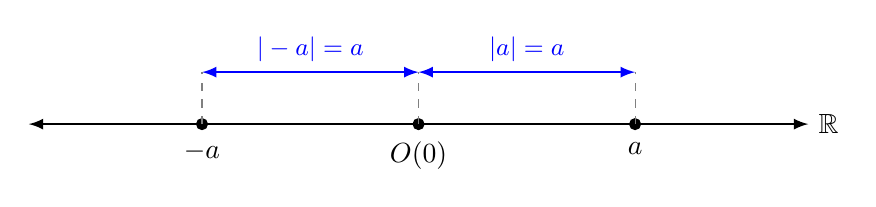
\begin{tikzpicture}[scale=1.1, >=latex]
  % 實數線與絕對值距離示意
  \draw[<->, thick] (-4.5, 0) -- (4.5, 0) node[right] {$\mathbb{R}$};
  
  \filldraw (0, 0) circle (1.8pt) node[below=3pt] {$O (0)$};
  \filldraw (-2.5, 0) circle (1.8pt) node[below=3pt] {$-a$};
  \filldraw (2.5, 0) circle (1.8pt) node[below=3pt] {$a$};
  
  \draw[<->, blue, thick] (-2.5, 0.6) -- (0, 0.6) node[midway, above] {\small $|-a| = a$};
  \draw[<->, blue, thick] (0, 0.6) -- (2.5, 0.6) node[midway, above] {\small $|a| = a$};
  
  \draw[dashed, gray] (-2.5, 0) -- (-2.5, 0.6);
  \draw[dashed, gray] (0, 0) -- (0, 0.6);
  \draw[dashed, gray] (2.5, 0) -- (2.5, 0.6);
\end{tikzpicture}
\caption{絕對值的幾何意義：數線上點到原點的距離}\label{fig:abs_dist}
\end{figure}

\subsection*{習題 3-8}\label{sec:ex3-8}
\addcontentsline{toc}{subsection}{習題 3-8}

試利用上面定義，證明下列各題（設 $a, b, x \in \mathbb{R}$）：
\begin{enumerate}[(i), leftmargin=2.5em]
  \item $\sqrt{a^2} = |a|$。
  \item $|ab| = |a| \cdot |b|$。
  \item $\left|\frac{a}{b}\right| = \frac{|a|}{|b|}$（$b \neq 0$）。
  \item $-|a| \le a \le |a|$。
  \item 若 $\delta > 0$，則 $|x| < \delta \iff -\delta < x < \delta$。
  \item 若 $\delta > 0$，則 $|x| > \delta \iff x > \delta$ 或 $x < -\delta$。
  \item $|a+b| \le |a| + |b|$（三角不等式）。
  \item $|a-b| \le |a| + |b|$。
  \item $\big||a| - |b|\big| \le |a+b|$。
  \item $\big||a| - |b|\big| \le |a-b|$。
\end{enumerate}
 % 第三章 數的概念
% =========================================================================
% 《高中數學實驗教材》第一冊（高一上） 
% 第四章 一次方程式
% =========================================================================

\section{一次方程式}\label{sec:ch4}

在小學的算術過程中，同學們都已學過整數和分數的加、減、乘、除這四種基本運算。一般說來，利用這四種基本運算（亦稱為四則運算）可以解答的種種「應用問題」統稱為「四則問題」，例如「龜兔問題」、「年齡問題」、「時鐘問題」、「盈虧問題」等等，相信同學們在小學裏一定做過不少。這些四則問題若能詳加解說，使同學們能確實把握其思路，從而用以訓練思考分析的能力，學起來是有趣的、有益處的。但是往往有許多同學只是去「記公式」，然後模仿地去「套公式」；假如題目稍加變化，就難免有花樣繁多、窮於應付之感了。當同學們在國中的數學課程中學到「一次方程式」後，以前的四則問題用一次方程式去解，可就簡單多了，而且無論題目如何變化，用一次方程式的解法是一致的，直截了當的。同樣是四則問題，為什麼代數的解法就會比算術的解法簡明有力呢？代數解法之所以優於算術解法的基本原理何在？這也就是本章要和同學們詳加討論的課題。

在第一節中，我們先舉些簡單的例子，把「代數的」與「算術的」兩種解法詳加分析比較。然後在第二節中把代數解法的基本原理——亦即「未知數」原理——徹底地加以剖析。因為這個看來簡單平凡的原理，也就是代數學的源起之一。所以同學們千萬要耐心細讀，務求徹底明白這一簡單的基本原理。只有心領神會、瞭若指掌的原理用起來才能得心應手，不是？

\subsection{四則問題與一次方程式的關係}\label{sec:4-1}

下面是幾個簡單的例子，它們的算術解法和代數解法都是同學們在小學和國中裏早已熟習的。我們現在把兩者加以比較分析，用以說明未知數的原理。

\begin{example}\label{ex:4-1-1}
雞兔同籠，共有 $8$ 個頭，$22$ 隻腳。問有雞幾隻？兔幾隻？
\end{example}

\paragraph{算術的解法：}
先假設 $8$ 隻都是兔，則應有腳 $4 \times 8 = 32$ 隻。然後每次用一隻雞去換一隻兔時，腳數相減 $4 - 2 = 2$，而我們的問題就是：「要用幾隻雞去換兔後，腳數才從 $32$ 減到 $22$？」故
\begin{equation}\label{eq:chicken_rabbit_arith}
  \text{雞數} = (4 \cdot 8 - 22) \div (4 - 2) = (32 - 22) \div 2 = 5 \dots\dots\dots
\end{equation}

\paragraph{相對應的代數解法是：}
令「雞數」為 $x$，則「兔數」為 $8-x$。由此去計算「腳數」，即得下述方程式：
\begin{equation}\label{eq:chicken_rabbit_alg}
  2 \cdot x + 4 \cdot (8-x) = 22 \dots\dots\dots
\end{equation}
\begin{align*}
  2x + 4 \cdot 8 - 4x &= 22 \quad \text{〔分配律〕} \\
  &\Downarrow \quad \text{移項} \\
  4 \cdot 8 - 22 &= (4 - 2)x \\
  &\Downarrow \\
  x &= (4 \cdot 8 - 22) \div (4 - 2) = 5 \dots\dots\dots
\end{align*}

\paragraph{比較與分析：}
在代數的解法中，我們引進一符號「$x$」用以表示「雞的數目」。利用它去計算腳數，即得等式 \eqref{eq:chicken_rabbit_alg}（叫做方程式）。然後從等式 \eqref{eq:chicken_rabbit_alg}，我們只要直截了當地運用「分配律」、「移項」等基本法則，即可解「雞數」$x$。再者，假如我們在運用分配律、移項等過程中，暫時不把 $4 \cdot 8$，$(4 \cdot 8 - 22)$ 及 $(4 - 2)$ 等算出來，〔亦即並不把 $4 \cdot 8$ 寫成 $32$，$(4 \cdot 8 - 22)$ 寫成 $10$，$(4 - 2)$ 寫成 $2$〕，只是利用括號把 $x$ 表出，即得
\begin{equation*}
  x = (4 \cdot 8 - 22) \div (4 - 2)
\end{equation*}
這就是在算術的解法中所用以計算雞數的公式了！

現在再讓我們看看算術解法中，是如何導出上述公式的。在算術中，我們逐步解釋 \eqref{eq:chicken_rabbit_arith} 式中所出現的「量」$4 \cdot 8$，$(4 \cdot 8 - 22)$ 及 $(4 - 2)$ 如下：
\begin{align*}
  4 \cdot 8 &= \text{假如 $8$ 隻全是兔所應有的腳數.} \\
  4 \cdot 8 - 22 &= \text{「$8$ 隻全是兔的腳數」和「現有腳數」的差額.} \\
  4 - 2 &= \text{每次以「一隻雞」換「一隻兔」所產生的腳數差.}
\end{align*}
最後，$\text{雞數} = \text{所需「替換」的次數} = (4 \cdot 8 - 22) \div (4 - 2)$。

由上述分析，同學們可以看出兩種解法間的異同與關係如下：
\begin{enumerate}[(i)]
  \item 代數中所依據的等式 \eqref{eq:chicken_rabbit_alg} 是腳數為 $22$ 的直接表示法，其中因為雞數是我們所要求取的未知數，所以只是用一個簡單的符號「$x$」代表之。然後由 \eqref{eq:chicken_rabbit_alg} 式，可以利用分配律、移項等基本法則，直截了當地導出 \eqref{eq:chicken_rabbit_arith} 式。解出 $x = 5$。
  \item 算術中所依據的是公式 \eqref{eq:chicken_rabbit_arith}，但是為了說明為什麼可以用公式 \eqref{eq:chicken_rabbit_arith} 去算出雞數，我們不得不逐步把公式中的每一步計算「找出」一個理由去解釋，這有時是頗費周折的。\footnote{假如同學們要追問算術中的公式 \eqref{eq:chicken_rabbit_arith} 是怎樣「想到的」？這裡有兩個答案：一個是教算術的老師用上述「一次方程式」的方法由 \eqref{eq:chicken_rabbit_alg} 式導出 \eqref{eq:chicken_rabbit_arith} 式，但是因為小學生沒學過「代數」，所以再逐步的把 \eqref{eq:chicken_rabbit_arith} 的量加以分析，解釋給小學生聽。另外一個答案可以叫做實驗歸納法，做題目的人可能用下面的想法：\\
  假如沒有雞，則有 $8$ 隻兔，腳數應該是 $8 \times 4 = 32$ 隻，\\
  假如只有一隻雞，則有 $7$ 隻兔，腳數應該是 $1 \times 2 + 7 \times 4 = 30$ 隻，（太多）\\
  假如是 $2$ 隻雞，則有 $6$ 隻兔，共有腳 $2 \times 2 + 6 \times 4 = 28$ 隻，（也太多）\\
  假如是 $3$ 隻雞，則有 $5$ 隻兔，共有腳 $3 \times 2 + 5 \times 4 = 26$ 隻，\\
  假如是 $4$ 隻雞，則有 $4$ 隻兔，共有腳 $4 \times 2 + 4 \times 4 = 24$ 隻，\\
  假如是 $5$ 隻雞，則有 $3$ 隻兔，共有腳 $5 \times 2 + 3 \times 4 = 22$ 隻，恰好。所以共有 $5$ 隻雞，$3$ 隻兔。但是仔細觀察上面計算，我們發現腳數自 $32, 30, 28, \dots, 24, 22$，慢慢自 $32$ 每次減 $2$，得到 $22$。這個事實用心去想，便能得到公式 \eqref{eq:chicken_rabbit_arith} 了。}
\end{enumerate}

\begin{example}\label{ex:4-1-2}
父年是子年的 $5$ 倍，$6$ 年後父年為子年的 $3$ 倍，問父子現在各幾歲？
\end{example}

\paragraph{代數解法：}
令「子年」為 $x$，則父年為 $5x$，$6$ 年後子年為 $x+6$，父年為 $5x+6$ 故有
\begin{equation}\label{eq:father_son_alg}
  3 \cdot (x+6) = 5x+6 \quad \text{（亦即：$6$ 年後父年為子年的 $3$ 倍）} \dots\dots\dots
\end{equation}
\begin{align*}
  &\Downarrow \quad \text{分配律} \\
  3x + 3 \cdot 6 &= 5x + 6 \\
  &\Downarrow \quad \text{移項} \\
  (3 \cdot 6 - 6) &= (5 - 3) \cdot x \\
  &\Downarrow \\
  \text{子年} &= (3 \cdot 6 - 6) \div (5 - 3) = 6 \dots\dots\dots \label{eq:father_son_arith} \\
  \text{父年} &= 5 \cdot 6 = 30 \text{。}
\end{align*}

\paragraph{算術解法：}
一如前面的例子，我們要把它由 \eqref{eq:father_son_alg} 所導出的式子中的「量」逐一加以解釋如下：

假如從「$6$ 年後的父年」減去 $3 \cdot 6$ 歲，即得「子現年」的 $3$ 倍。也就是說從「父現年」減去 $(3 \cdot 6 - 6)$ 歲，即得「子現年」的 $3$ 倍，但是「父現年」是「子現年」的 $5$ 倍，故 $(3 \cdot 6 - 6)$ 恰為子現年的 $(5 - 3)$ 倍，即
\begin{equation*}
  \text{子年} = (3 \cdot 6 - 6) \div (5 - 3) = 6
\end{equation*}

同學們看得懂上面的「解釋」沒有？如果不懂，請不要灰心，看一看下面我們所作的剖析。

$6$ 年後的子年的 $3$ 倍，包括兩部份：
\begin{enumerate}[(1)]
  \item 子現年的 $3$ 倍和
  \item $6 \times 3 = 18$。
\end{enumerate}

$6$ 年後的父年也包括兩部份：
\begin{enumerate}[$(1')$]
  \item 現在子年的 $5$ 倍和
  \item $6$。
\end{enumerate}

\begin{figure}[htbp]
\centering
\begin{tikzpicture}[scale=0.88, >=latex]
  % 第一行：子現年 3 倍 + 18
  \foreach \i in {0, 1, 2} {
    \draw[thick] (\i*2.2, 1.8) rectangle ++(2.0, 0.7);
    \node at (\i*2.2+1.0, 2.15) {\small 子現年};
  }
  % 虛線分割與延伸
  \draw[thick, densely dashed] (6.6, 1.8) -- (6.6, 2.5);
  % 上方 18 的尺寸標註
  \draw[|<->|, thick] (6.6, 2.85) -- (12.2, 2.85) node[midway, fill=white] {\small $18$};
  % 下方 12 與 6 的尺寸標註
  \draw[|<->|, thick] (6.6, 1.3) -- (10.4, 1.3) node[midway, fill=white] {\small $12$};
  \draw[|<->|, thick] (10.4, 1.3) -- (12.2, 1.3) node[midway, fill=white] {\small $6$};
  
  % 第二行：子現年 5 倍 + 6
  \foreach \i in {0, 1, 2, 3, 4} {
    \draw[thick] (\i*2.2, 0) rectangle ++(2.0, 0.7);
    \node at (\i*2.2+1.0, 0.35) {\small 子現年};
  }
  % 虛線分割
  \draw[thick, densely dashed] (11.0, 0) -- (11.0, 0.7);
  % 最右側 6 的尺寸標註
  \draw[|<->|, thick] (10.4, -0.45) -- (12.2, -0.45) node[midway, fill=white] {\small $6$};
  
  % 垂直輔助對齊虛線
  \draw[gray, dotted] (6.6, 2.9) -- (6.6, -0.5);
  \draw[gray, dotted] (10.4, 1.4) -- (10.4, -0.5);
  \draw[gray, dotted] (12.2, 2.9) -- (12.2, -0.5);
\end{tikzpicture}
\caption{年齡問題之圖解算術}\label{fig:age_diagram}
\end{figure}

由\cref{fig:age_diagram}，可以看出子現年就是 $12 \div 2 = 6$。上面的解法，在小學中叫做圖解算術。同學們可以注意到，利用圖解算術，事實上便相當於解方程式。這也是為什麼利用圖解方法，往往可以很清楚地解決四則問題的原因。

從上面二個簡單的例子，同學們可以看出，在代數的解法上，「年齡問題」和「雞兔問題」可以說毫無分別，直截了當。但是算術的解法卻得一步步地依題意找「解釋」，相互比較下，顯然代數的解法遠較算術的解法直截而且簡明，在習題中，我們將列舉許多其他類型的「四則問題」，讓同學們自行比較分析兩種解法，這是一種有趣的練習。

\subsection*{習題 4-1}\label{sec:ex4-1}
\addcontentsline{toc}{subsection}{習題 4-1}

\begin{enumerate}[1.]
  \item 甲乙兩人共有 $100$ 元，甲比乙多 $28$ 元，問甲、乙各有多少錢？
  \item 某數加 $5$ 後乘 $4$ 再減 $2$，等於這個數的 $7$ 倍，試求這個數。
  \item 在溫度計上，華氏與攝氏所示度數相同的溫度是幾度？
  \item 有一個二位數，它的十位數字加上 $1$ 為個位數的兩倍，十位與個位數置相換後\footnote{此處「數置」實為「位置」之排印訛字，見\hyperref[sec:master_errata_notes]{目錄前勘誤表}。}，得一新數，舊數比新數大 $18$，問原來數是多少？\label{item:ex4-1-4}
  \item 某班男女同學共有 $45$ 人，在某次考試中全班平均分數是 $72$ 分，男生的平均分數是 $70$ 分，女生的平均分數是 $75$ 分，求男生、女生各有多少人？
  \item 用算數及代數兩種方法做下面的題目。\\
  四點鐘到五點鐘之間，什麼時候時針與分針 (1) 重合，(2) 成直角，(3) 成直線。
  \item[$*7.$] 某人放款 $5000$ 元，其一部分的利率為 $6\%$，另一部分是 $4\%$，平均利率為 $5\frac{1}{2}\%$，問這兩部份各多少？（代數與算術兩種方法）。
\end{enumerate}

\subsection{「未知數」原理——數系通性的應用}\label{sec:4-2}

\subsubsection*{甲、為什麼用一次方程式去解四則問題就遠比算術的解法來得簡單明瞭呢？}\label{subsec:4-2-a}

從表面上看來，好像只是因為在代數的解法中我們引入了「未知數」（通常用 $x$、$y$、$z$ 表之）。因此如果不去仔細分析深究，也許有人就會說：「代數之所以優於算術，是因為代數中有了『未知數』$x$、$y$、$z$ 這些符號的幫助。」這一點雖然不錯，但卻不是根本的原因。譬如在例 1 中用 $x$ 表示「雞數」，這只是一個簡寫，筆劃少些。$x$、$y$、$z$，這些符號本身並無任何神妙之處。再者，當我們引進「未知數」後，按題意去列出方程式（如例 1 中的式子，例 2 中的式子）。這也是利用符號把題義加以翻譯而已。換句話說，方程式只是把題目本身用簡單的符號寫成「看起來清楚些的式子」罷了！代數解法的真正關鍵在於「可以從方程式去解出未知數」這一點上！而且這種解法是直截了當的，簡單明瞭的。

那麼從方程式去解出未知數的原理何在呢？這也就是我們在第一節要和大家仔細討論的。簡括來說：引入未知數，從方程式去解題的基本原理在於活用上一章中向大家介紹的數系基本性質。

\subsubsection*{乙、一元一次方程式的解法}\label{subsec:4-2-b}

一元一次方程式是代數方程式中最簡單的，它們的解法，同學們業已在國中代數課程中學過。（方程式的「元」數和「次」數的意義，也是在國中代數即已教過的，但在本書第五章中將再加解釋。）我們在這裏和大家討論其解法的原理。

譬如我們由某一問題，得出下列方程式：
\begin{equation}\label{eq:linear_demo_1}
  2 \left[ \frac{1}{3} (2x-5) - 9x(4-3) \right] - 15 = 100 - 20x \dots\dots\dots
\end{equation}
上述算式叫一個小學生去做可能有些棘手。因為老師教他的是先算小括號，再算中括號，……等。而現在有一個小括號是 $(2x-5)$，它是算不出來的，因而也就沒辦法和 $\frac{1}{3}$ 相乘，以下更是無從著手了。那麼為什麼中學生就有辦法去算上述算式，而且從而可以解出「$x=?$」呢？說穿了是簡單不過的：

\begin{quote}
「『$x$』雖然是個未知數，一個我們不知道它等於多少的數。但是只要它是一個「數」，它在運算上就滿足上一章所列述的如分配律、結合律、交換律這些基本通性，因為這些基本性質是對任何數都成立的！」
\end{quote}

所以我們不去管 $(2x-5)$ 等於多少！
\begin{equation*}
  \frac{1}{3}(2x-5) = \frac{1}{3} \cdot 2 \cdot x - \frac{1}{3} \cdot 5 = \frac{2}{3}x - \frac{5}{3}
\end{equation*}
總是成立！所以我們只要懂得去活用有理數系中那些看來又簡單又平凡的基本通性，我們就不再擔心某些小括號或中括號算不出來了。譬如上述 \eqref{eq:linear_demo_1} 式就可逐步化簡成
\begin{equation}\label{eq:linear_demo_2}
  \frac{4}{3}x - \frac{10}{3} - 18x - 15 = 100 - 20x \dots\dots\dots
\end{equation}
（請同學們檢查一下上述化簡過程中用到那些基本性質）。

將 \eqref{eq:linear_demo_2} 式再加上「移項」和「集項」\footnote{移項的原理在於：「等式兩端同加一數，則所得者依然為一等式。」「集項時我們用了加法交換律和分配律。」}，即得
\begin{equation*}
  \left( \frac{4}{3} - 18 + 20 \right) x = 100 + 15 + \frac{10}{3}
\end{equation*}
即
\begin{equation*}
  \frac{10}{3}x = \frac{355}{3}
\end{equation*}
故可解得
\begin{equation*}
  x = \frac{71}{2} \text{。}
\end{equation*}

\subsubsection*{乙、運用數系的通性去解方程式}\label{subsec:4-2-b2}

說明了是一個淺顯而自然的方法，正因為這種解法直接而自然，它是一個簡明的好方法，這裏有一個還算恰當的譬喻：用算術的解法去解四則問題有如練了好些套「花拳繡腿」，演來招式繁多，但是不切實際。而利用數系的通性，列方程式去解四則題，則有如關公的青龍偃月刀，簡單明瞭地砍個正著，過關斬將一切也就迎刃而解了。再者，我們要提醒大家，在一次方程式中，只可以說是數系通性的牛刀小試，它們的妙用還多著呢？希望同學們隨時對這些簡潔的數系通性的種種用法多加注意，用心去體會。

\subsection*{習題 4-2}\label{sec:ex4-2}
\addcontentsline{toc}{subsection}{習題 4-2}

\begin{enumerate}[1.]
  \item 如果 $ax+b=cx+d$，在 $x=x_1$ 和 $x=x_2$ ($x_1 \neq x_2$) 時都成立。那麼 $a=c$，$b=d$。
  \item $a, b, c, d$ 是不同的實數，解下列各方程式：
  \begin{enumerate}[(i)]
    \item $ax+c=bx+d$。
    \item $a(x+b)-b(x+a)=a^2-b^2$。
  \end{enumerate}
  \item 如果 $x=-\frac{1}{2}$ 是方程式 $\frac{a(x+2)}{3} - \frac{2-ax}{4} = -2$ 的根，求 $a$。
  \item 試證一數之一半加上 $a$，除以 $n$，減掉 $\frac{1}{n}$，乘 $2n$，再減 $2a-2$，就是原數。
  \item 解下列方程式：
  \begin{enumerate}[(i)]
    \item $\{ [ (5x+8) \cdot 4 + 7x ] \cdot 3 + 9x \} \cdot 4 = 5x$。\label{item:ex4-2-5-1}
    \item $5 [ 3x - 9(5x+7) ] - 6x = 2$。
  \end{enumerate}
  \item $a, b, c$ 是不等於 $0$ 的實數，解下列各方程式：
  \begin{enumerate}[(i)]
    \item $\dfrac{x+a}{b} - \dfrac{x-b}{a} = 2$。
    \item $\dfrac{x-a}{bc} - \dfrac{x+c}{ab} = \dfrac{2(b-c)}{ab} - \dfrac{x+b}{ac}$。
    \item $\dfrac{x}{a-b} = \dfrac{x-b}{a}$，($a \neq b$)。
  \end{enumerate}
  \item 試解 $(a+2)(a-5)x = a+11-12(x+1)$。\\
  （提示：須分成 (i) $a \neq 1, a \neq 2$ \quad (ii) $a=1$ \quad (iii) $a=2$ 三種情形討論）
  \item 某生計算方程式 $6x+10=9x+15$。依下列步驟，
  \begin{align*}
    2(3x+5) &= 3(3x+5) \\
    2 &= 3
  \end{align*}
  得到矛盾，請找出錯誤。
\end{enumerate}

\subsection{二元、三元一次聯立方程式}\label{sec:4-3}

當未知數不只是一個時，我們即得多元方程式。一般說來，方程式的個數和未知數的個數常常是相等的。在這一節中我們將把上節所提出的原理，進一步來討論如何來解二元、三元聯立方程式。（多元一次聯立方程式的一般性理論，將留待高三下和行列式的理論一併討論。）首先，讓我們來看幾個例子：

\subsubsection*{甲、聯立方程式的實例}\label{subsec:4-3-a}

\begin{example}\label{ex:4-3-1}
雞兔同籠，共有 $8$ 個頭，$22$ 隻腳。問有雞幾隻？兔幾隻？
\end{example}

這一題我們在一元一次方程式那一節業已詳加討論。那時候我們的解法，是令雞數為 $x$，而將兔數算出為 $8-x$。

對於上述問題一個更自然更直接的解法是令雞數為 $x$，兔數為 $y$，則由「頭數為 $8$」及「腳數為 $22$」兩個條件，分別得下列兩個方程式，即
\begin{equation}\label{eq:sim_cr_1}
  x+y = 8 \dots\dots\dots
\end{equation}
\begin{equation}\label{eq:sim_cr_2}
  2x+4y = 22 \dots\dots\dots
\end{equation}
假如將 $\eqref{eq:sim_cr_1} \cdot 4 - \eqref{eq:sim_cr_2}$，即得
\begin{align*}
  (4-2)x &= 4 \cdot 8 - 22 \\
  x &= (4 \cdot 8 - 22) \div (4-2)
\end{align*}
這便是 \S 4-1 例 1 中的算式。

譬如我們把上述題目改成下列「奇禽怪獸同籠」問題如下：

\begin{example}\label{ex:4-3-2}
有「九頭奇禽」和「四頭怪獸」同籠，共有頭 $75$ 個，腳 $26$ 個。問有九頭奇禽幾隻？四頭怪獸幾隻？\footnote{「九頭奇禽」顧名思義乃是九頭兩腳的一種飛禽，而「四頭怪獸」應當是一種「四頭四腳」的走獸。這樣的奇禽怪獸相信大家都沒見過，但為了舉例說明起見，做幾個塑膠的，想必不難。}
\end{example}

\begin{solution*}
上述例題和雞兔同籠問題完全屬於同一類型。例如用二元一次聯立方程式去解，我們只要令禽數為 $x$，獸數為 $y$。則有
\begin{equation}\label{eq:monster_1}
  9x+4y = 75 \dots\dots\dots
\end{equation}
\begin{equation}\label{eq:monster_2}
  2x+4y = 26 \dots\dots\dots
\end{equation}
當然我們可以先由 \eqref{eq:monster_1} 式解出 $y$（或 $x$），用以代入 \eqref{eq:monster_2} 式，即得一個一元一次方程式
\begin{equation}\label{eq:monster_sub}
  2x + 4 \left( \frac{75-9x}{4} \right) = 26 \dots\dots\dots
\end{equation}
從 \eqref{eq:monster_sub} 式化簡，即得
\begin{equation*}
  2x - 9x = 26 - 75
\end{equation*}
即
\begin{equation*}
  -7x = -49
\end{equation*}
故
\begin{equation}\label{eq:monster_sol_x}
  x = \frac{-49}{-7} = 7 \dots\dots\dots
\end{equation}
將 $x=7$ 代入 \eqref{eq:monster_2} 式，即得
\begin{equation*}
  14 + 4y = 26
\end{equation*}
即
\begin{equation*}
  4y = 12
\end{equation*}
故
\begin{equation}\label{eq:monster_sol_y}
  y = \frac{12}{4} = 3 \dots\dots\dots
\end{equation}
但是和前例一樣，上述聯立方程式 \eqref{eq:monster_1} 和 \eqref{eq:monster_2} 的更直接更簡便的解法是將 \eqref{eq:monster_1} 式減去 \eqref{eq:monster_2} 式，即可「消去 $y$」：
\begin{equation*}
\begin{array}{r@{\quad}l}
  & 9x + 4y = 75 \\
  -) & 2x + 4y = 26 \\ \hline
  & 7x + 0y = 49
\end{array}
\end{equation*}
馬上就得出 $x=7, y=3$。
\end{solution*}

\begin{example}\label{ex:4-3-3}
有九頭奇禽和雞兔同籠，共有頭 $26$ 個，尾 $10$ 條，腳 $30$ 隻。問有九頭奇禽幾隻？雞幾隻？兔幾隻？（按：它們都是單尾動物）。
\end{example}

\begin{solution*}
令九頭禽之數為 $x$，雞數為 $y$，兔數為 $z$，則有
\begin{equation}\label{eq:three_var_1}
  9x + y + z = 26 \dots\dots\dots
\end{equation}
\begin{equation}\label{eq:three_var_2}
  x + y + z = 10 \dots\dots\dots
\end{equation}
\begin{equation}\label{eq:three_var_3}
  2x + 2y + 4z = 30 \dots\dots\dots
\end{equation}
將 \eqref{eq:three_var_1} 式和 \eqref{eq:three_var_2} 式相減\footnote{原書印為「由 $(1)+(2)+(3)$，即得」，實為標籤沿用筆誤，應為 \eqref{eq:three_var_1} 與 \eqref{eq:three_var_2} 兩式運算，見\hyperref[sec:master_errata_notes]{目錄前勘誤表}。}，即得
\begin{equation*}
  9x - x = 26 - 10 \text{，}
\end{equation*}
即
\begin{equation*}
  8x = 16 \text{，} \quad \text{故 } x=2 \text{。}
\end{equation*}
由 $\eqref{eq:three_var_3} - 2 \times \eqref{eq:three_var_2}$，即得
\begin{equation*}
  4z - 2z = 30 - 20 \text{，}
\end{equation*}
即
\begin{equation*}
  2z = 10 \text{，} \quad \text{故 } z=5 \text{。}
\end{equation*}
將 $x=2, z=5$ 代入 \eqref{eq:three_var_2} 式，即得
\begin{equation*}
  2 + y + 5 = 10 \text{，}
\end{equation*}
即
\begin{equation*}
  y = 10 - 2 - 5 \text{，} \quad \text{故 } y=3 \text{。}
\end{equation*}
所以有九頭奇禽 $2$ 隻，雞 $3$ 隻，兔 $5$ 隻。
\end{solution*}

\subsection*{習題 4-3}\label{sec:ex4-3}
\addcontentsline{toc}{subsection}{習題 4-3}

\begin{enumerate}[1.]
  \item 甲、乙合做一項工程，十天可以完成，兩人合做 $7$ 天後，甲因病休工，乙再獨做 $5$ 天才完工，問兩人單獨工作，各需要幾天才可以做完？
  \item 某班男女同學共有 $45$ 人，統計了戴眼鏡的情形，發現下列事實，即女同學中有 $\frac{1}{4}$ 戴眼鏡，男同學有 $\frac{1}{7}$，全班共有 $\frac{1}{5}$ 的同學戴眼鏡，問戴眼鏡的男女同學各有多少人？
  \item 少棒隊甲、乙兩隊各與丙隊比賽 $26$ 場，甲隊贏丙隊的場數是乙隊贏丙隊的三倍，乙隊輸給丙隊的場數是甲隊輸給丙隊的 $9$ 倍，試問甲、乙隊各贏丙隊幾場？
  \item 某河上橫跨一橋，由上游垂直划來兩船，船速都是每秒 $3$ 尺，第一艘船長 $20$ 尺，從橋的一側划到另一側需時 $10$ 秒，另一艘船長 $14$ 尺，需要 $8\frac{1}{2}$ 秒，划到另一側，問橋寬和水流的速度。
  \item 要合成 $40\%$ 的食鹽水 $900$ 公升，需要 $15\%$ 和 $60\%$ 的食鹽水各幾公升？
  \item 一室中有男女一羣，從男子眼中看去，女人比男人少一人，從女子眼中看去，男人比女人多一倍，問男女各多少人？
  \item 犬走 $4$ 步，兔走 $5$ 步，而犬走 $2$ 步的距離，等於兔走 $3$ 步，兔先走 $100$ 步後，犬由後追兔，問犬追幾步，才能追到？
  \item 有一工程，如甲、乙、丙三人合作，$10$ 天可成，如乙、丙合作，$15$ 天可成，如甲做 $15$ 天，餘下由丙來做，要再 $30$ 天才做成，問甲、乙、丙獨做，各需幾天完成？
\end{enumerate}

\subsubsection*{乙、二元一次聯立方程式的解法}\label{subsec:4-3-b}

二元一次聯立方程式經過化簡後，可以寫成下列型式：
\begin{equation}\label{eq:2var_gen_1}
  a_1 x + b_1 y = c_1 \dots\dots\dots
\end{equation}
\begin{equation}\label{eq:2var_gen_2}
  a_2 x + b_2 y = c_2 \dots\dots\dots
\end{equation}
在國中代數裏，我們即已學過上列聯立方程式的兩種解法：「代入法」和「消去法」。

\paragraph{代入法：}
代入法是從一式解出 $x$（或 $y$）代入另一式，即得一個 $y$（或 $x$）的一元一次方程式，從而解得 $y$（或 $x$）。再將解得的 $y$（或 $x$）代入兩式之一，即可解得 $x$（或 $y$）。以上述普遍型式為例，即由 \eqref{eq:2var_gen_1} 式解出 $x$，得
\begin{equation*}
  x = \frac{c_1 - b_1 y}{a_1} \quad \text{（當然要在 $a_1 \neq 0$ 時才可以這樣做）}
\end{equation*}
代入 \eqref{eq:2var_gen_2} 式，得
\begin{equation*}
  a_2 \left( \frac{c_1 - b_1 y}{a_1} \right) + b_2 y = c_2 \text{。}
\end{equation*}
化簡後，即得
\begin{equation*}
  (a_1 b_2 - a_2 b_1) y = a_1 c_2 - a_2 c_1 \text{。}
\end{equation*}
當 $(a_1 b_2 - a_2 b_1) \neq 0$ 時，即得
\begin{equation*}
  y = \frac{a_1 c_2 - a_2 c_1}{a_1 b_2 - a_2 b_1} \text{。}
\end{equation*}
將上述 $y$ 的值代入 \eqref{eq:2var_gen_1} 式，即得
\begin{equation*}
  a_1 x + b_1 \cdot \frac{a_1 c_2 - a_2 c_1}{a_1 b_2 - a_2 b_1} = c_1 \text{。}
\end{equation*}
通分後，成
\begin{align*}
  a_1 (a_1 b_2 - a_2 b_1) x &= c_1 \cdot (a_1 b_2 - a_2 b_1) - b_1 \cdot (a_1 c_2 - a_2 c_1) \\
  &= c_1 a_1 b_2 - c_1 a_2 b_1 - b_1 a_1 c_2 + b_1 a_2 c_1 \\
  &= a_1 (c_1 b_2 - c_2 b_1) \text{。}
\end{align*}
故有
\begin{equation*}
  x = \frac{c_1 b_2 - c_2 b_1}{a_1 b_2 - a_2 b_1} \text{。}
\end{equation*}

\paragraph{消去法：}
由 $a_2 \cdot \eqref{eq:2var_gen_1} - a_1 \cdot \eqref{eq:2var_gen_2}$，即可消去 $x$。即
\begin{equation*}
\begin{array}{r@{\quad}l}
  & a_2 \cdot a_1 x + a_2 \cdot b_1 y = a_2 \cdot c_1 \\
  -) & a_1 \cdot a_2 x + a_1 \cdot b_2 y = a_1 \cdot c_2 \\ \hline
  & (a_2 b_1 - a_1 b_2) y = a_2 c_1 - a_1 c_2
\end{array}
\end{equation*}
如 $(a_2 b_1 - a_1 b_2) \neq 0$ 時，即得
\begin{equation*}
  y = \frac{a_2 c_1 - a_1 c_2}{a_2 b_1 - a_1 b_2} = \frac{a_1 c_2 - a_2 c_1}{a_1 b_2 - a_2 b_1} \text{。}
\end{equation*}
同理，由 $b_2 \cdot \eqref{eq:2var_gen_1} - b_1 \cdot \eqref{eq:2var_gen_2}$，即可消去 $y$，得
\begin{equation*}
  x = \frac{c_1 b_2 - c_2 b_1}{a_1 b_2 - a_2 b_1} \text{。}
\end{equation*}

由上述討論可知，當 $a_1 b_2 - a_2 b_1 \neq 0$ 時，聯立方程式
\begin{equation*}
\begin{cases}
  a_1 x + b_1 y = c_1 \\
  a_2 x + b_2 y = c_2
\end{cases}
\end{equation*}
的解，可由下述公式寫出，即
\begin{equation}\label{eq:2var_cramer_formula}
\begin{cases}
  x = \dfrac{c_1 b_2 - c_2 b_1}{a_1 b_2 - a_2 b_1} \\[1.2em]
  y = \dfrac{a_1 c_2 - a_2 c_1}{a_1 b_2 - a_2 b_1}
\end{cases}
\end{equation}

\begin{example}\label{ex:4-3-4}
解聯立方程式
\begin{equation}\label{eq:ex_2var_1}
  2x + 3y = 7 \dots\dots\dots
\end{equation}
\begin{equation}\label{eq:ex_2var_2}
  3x - 2y = 5 \dots\dots\dots
\end{equation}
\end{example}

\begin{solution*}
用代入法：由 \eqref{eq:ex_2var_1} 得 $x = \frac{7-3y}{2}$，代入 \eqref{eq:ex_2var_2}
\begin{equation*}
  3 \cdot \left( \frac{7-3y}{2} \right) - 2y = 5
\end{equation*}
即
\begin{equation*}
  21 - 13y = 10
\end{equation*}
所以
\begin{equation*}
  y = \frac{11}{13}
\end{equation*}
代入 \eqref{eq:ex_2var_1} 解出
\begin{equation*}
  x = \frac{29}{13} \text{。}
\end{equation*}

再用消去法：
\begin{equation*}
  \eqref{eq:ex_2var_1} \times 3 - \eqref{eq:ex_2var_2} \times 2 \qquad 13y = 11
\end{equation*}
所以
\begin{equation*}
  y = \frac{11}{13} \text{。}
\end{equation*}
\end{solution*}

\begin{example}\label{ex:4-3-5}
試解
\begin{equation}\label{eq:ex_param_1}
  (a-3)x - 2y = 2a \dots\dots\dots
\end{equation}
\begin{equation}\label{eq:ex_param_2}
  3x + (2a+1)y = a-2 \dots\dots\dots
\end{equation}
並就 $a$ 的值討論之。
\end{example}

\begin{solution*}
$\eqref{eq:ex_param_1} \cdot (2a+1) + \eqref{eq:ex_param_2} \cdot 2$
\begin{equation*}
  (2a^2 - 5a + 3)x = 4a^2 - 4 \footnote{此處原書展開計算訛誤：常數項實為 $2a(2a+1)+2(a-2) = 4a^2+4a-4$，原書脫漏 $+4a$，導致後續對 $a=1$ 之討論產生謬誤，詳見\hyperref[sec:master_errata_notes]{目錄前勘誤表}。}
\end{equation*}
\begin{equation*}
  \therefore \quad (2a-3)(a-1)x = 4(a+1)(a-1)
\end{equation*}
$\eqref{eq:ex_param_1} \cdot 3 - \eqref{eq:ex_param_2} \cdot (a-3)$
\begin{equation*}
  (2a^2 - 5a + 3)y = -(a^2 + 5a - 6)
\end{equation*}
\begin{equation*}
  \therefore \quad (2a-3)(a-1)y = -(a+6)(a-1)
\end{equation*}

當 $(2a-3)(a-1) \neq 0$ 時，有一組解
\begin{equation*}
\begin{cases}
  x = \dfrac{4(a+1)(a-1)}{(2a-3)(a-1)} \\[1.2em]
  y = \dfrac{-(a+6)(a-1)}{(2a-3)(a-1)}
\end{cases}
\end{equation*}

當 $a=1$ 時，\eqref{eq:ex_param_1}、\eqref{eq:ex_param_2} 式可寫成 $x+y=-1$，故有無窮多組解。\footnote{原書此處斷定「有無窮多組解」，實為前述計算錯誤所致之矛盾結論。事實上當 $a=1$ 時，原方程 \eqref{eq:ex_param_1} 化為 $x+y=-1$，而 \eqref{eq:ex_param_2} 化為 $3x+3y=-1 \implies x+y=-\frac{1}{3}$，兩者矛盾無解。}

當 $a = \frac{3}{2}$ 時，\eqref{eq:ex_param_1}、\eqref{eq:ex_param_2} 式變成
\begin{equation*}
\begin{cases}
  3x+4y = -6 \\
  3x+4y = -\dfrac{7}{2} \text{，}
\end{cases}
\quad \text{故無解。}
\end{equation*}
\end{solution*}

\subsection*{習題 4-4}\label{sec:ex4-4}
\addcontentsline{toc}{subsection}{習題 4-4}

\begin{enumerate}[1.]
  \item 解下列聯立方程式，並討論之。
  \begin{enumerate}[(1)]
    \item 
    $\begin{cases}
      ax+by = c \\
      px = qy
    \end{cases}$
    \item 
    $\begin{cases}
      (x-a)(a+b) = (u-b)(y-a) \\
      \dfrac{x}{a^3-b^3} = \dfrac{y}{a^3+b^3}
    \end{cases}$\footnote{原書第一式中印為 $(u-b)$，顯為英文字母 $a$ 字模殘損缺頂所致，或為 $(a-b)(y-a)$ 之排印訛植，見\hyperref[sec:master_errata_notes]{目錄前勘誤表}。}\label{item:ex4-4-1-2}
    \item 
    $\begin{cases}
      \left(\dfrac{1}{a}+\dfrac{1}{b}\right)x + \left(\dfrac{1}{a}-\dfrac{1}{b}\right)y = 4 \\
      \dfrac{x}{a+b} + \dfrac{y}{a-b} = 2
    \end{cases}$
    \item 
    $\begin{cases}
      \dfrac{x+y}{xy} = 3 \\
      \dfrac{x-y}{xy} = 1
    \end{cases}$\footnote{原書第二式印為 $\frac{x-y}{xy} = i$，實為阿拉伯數字「$1$」之字模印損殘跡，非虛數單位 $i$，見\hyperref[sec:master_errata_notes]{目錄前勘誤表}。}\label{item:ex4-4-1-4}
    \item 
    $\begin{cases}
      \dfrac{x+y}{3} + \dfrac{y-x}{2} = 5 \\
      \dfrac{x}{2} + \dfrac{x+y}{9} = 7
    \end{cases}$
    \item 
    $\begin{cases}
      \dfrac{x-y}{x+y} = \dfrac{m-n}{m+n} \quad (m+n \neq 0) \text{。} \\
      nx + my = 1
    \end{cases}$
    \item 
    $\begin{cases}
      2y = 2 \\
      4x + \dfrac{1}{y} = 3
    \end{cases}$
    \item 
    $\begin{cases}
      \dfrac{x}{2} + \dfrac{y}{3} = 1+x \\
      \dfrac{x}{3} + \dfrac{y}{2} = 1+y
    \end{cases}$
  \end{enumerate}
\end{enumerate}

\subsubsection*{丙、三元一次聯立方程式}\label{subsec:4-3-c}

一個三元一次聯立方程式，經過化簡後，可以寫成下列型式：
\begin{equation}\label{eq:3var_gen_1}
  a_1 x + b_1 y + c_1 z = d_1 \dots\dots\dots
\end{equation}
\begin{equation}\label{eq:3var_gen_2}
  a_2 x + b_2 y + c_2 z = d_2 \dots\dots\dots
\end{equation}
\begin{equation}\label{eq:3var_gen_3}
  a_3 x + b_3 y + c_3 z = d_3 \dots\dots\dots
\end{equation}
同樣地，我們也可以有代入法和消去法這兩種解法，譬如我們由 \eqref{eq:3var_gen_1} 式解出 $x = \frac{d_1 - b_1 y - c_1 z}{a_1}$，代入 \eqref{eq:3var_gen_2}、\eqref{eq:3var_gen_3} 兩式，化簡後，即得只含有 $y$、$z$ 的二元聯立方程式，然後再用二元聯立方程式的解法求出 $y$、$z$ 來，再代入上式即得 $x$，這就是代入法。但是通常在計算中，代入法往往不如消去法來得簡便，所以三元以上的聯立方程式，我們通常都用消去法直接去解。消去法的一般討論留待下節，現在舉些例子說明如下：

\begin{example}\label{ex:4-3-6}
解聯立方程式
\begin{equation}\label{eq:3var_ex1_1}
  x+y = 10 \dots\dots\dots
\end{equation}
\begin{equation}\label{eq:3var_ex1_2}
  y+z = -2 \dots\dots\dots
\end{equation}
\begin{equation}\label{eq:3var_ex1_3}
  z+x = 2 \dots\dots\dots
\end{equation}
\end{example}

\begin{solution*}
由 $\eqref{eq:3var_ex1_1} + \eqref{eq:3var_ex1_2} + \eqref{eq:3var_ex1_3}$，即得
\begin{equation*}
  2 \cdot (x+y+z) = 10
\end{equation*}
即
\begin{equation}\label{eq:3var_ex1_sum}
  x+y+z = 5 \dots\dots\dots
\end{equation}
$\eqref{eq:3var_ex1_sum} - \eqref{eq:3var_ex1_1}$，即得 $z=-5$。\\
$\eqref{eq:3var_ex1_sum} - \eqref{eq:3var_ex1_2}$，即得 $x=7$。\\
$\eqref{eq:3var_ex1_sum} - \eqref{eq:3var_ex1_3}$，即得 $y=3$。
\end{solution*}

\begin{example}\label{ex:4-3-7}
解聯立方程式
\begin{equation}\label{eq:3var_ex2_1}
  x+3y+2z = 11 \dots\dots\dots
\end{equation}
\begin{equation}\label{eq:3var_ex2_2}
  2x+y+3z = 14 \dots\dots\dots
\end{equation}
\begin{equation}\label{eq:3var_ex2_3}
  x+y+z = 6 \dots\dots\dots
\end{equation}
\end{example}

\begin{solution*}
由 $\eqref{eq:3var_ex2_1} - \eqref{eq:3var_ex2_3}$，得
\begin{equation}\label{eq:3var_ex2_elim1}
  2y+z = 5 \dots\dots\dots
\end{equation}
$\eqref{eq:3var_ex2_2} - 2 \cdot \eqref{eq:3var_ex2_3}$，得
\begin{equation}\label{eq:3var_ex2_elim2}
  -y+z = 2 \dots\dots\dots
\end{equation}
$\eqref{eq:3var_ex2_elim1} - \eqref{eq:3var_ex2_elim2}$，即得 $3y = 3$，故 $y=1$，代入 \eqref{eq:3var_ex2_elim2}，得 $z=3$。\\
將 $y=1, z=3$ 代入 \eqref{eq:3var_ex2_3}，即得 $x=2$。
\end{solution*}

\subsection*{習題 4-5}\label{sec:ex4-5}
\addcontentsline{toc}{subsection}{習題 4-5}

\begin{enumerate}[1.]
  \item 解聯立方程式
  \begin{equation*}
  \begin{cases}
    x+2y+3z = 14 \\
    3x+y+2z = 11 \\
    2x+3y+z = 11
  \end{cases}
  \end{equation*}
  \item 設 $a \neq 1$，求解
  \begin{equation*}
  \begin{cases}
    ax+y+z = 1 \\
    x+ay+z = 1 \\
    x+y+az = 1
  \end{cases}
  \end{equation*}
  \item 解
  \begin{equation*}
  \begin{cases}
    \dfrac{x+2y}{3} = \dfrac{3y+4z}{5} = \dfrac{5z+6x}{7} \\[1em]
    3(x+y+z) = 7
  \end{cases}
  \end{equation*}
  \item 一個三位數的十位數字等於個位與百位數字的和，而它的個位與十位數字的和是 $8$ 如果個位與百位數字互換，這個數就增加 $99$，求這個數。
  \item 有一個三位數，各位數字的和是 $18$，交換個位數字與百位數字後就比原數大 $495$，交換十位數字與百位數字，就比原數大 $630$，求這個數。
  \item 三數的和是 $51$，第一數除以第二數，得到商數 $2$，餘數 $5$，第二數除以第三數，得到商數 $3$，餘數 $2$，問各數多少？
\end{enumerate}

\subsection{二階、三階行列式及二元、三元聯立方程式的初步討論}\label{sec:4-4}

\subsubsection*{甲、二階行列式與二元聯立方程式}\label{subsec:4-4-a}

在 \S 4-3 乙中，我們初步地討論一個典型的二元一次聯立方程式的解法，我們的結論是：當 $a_1 b_2 - a_2 b_1 \neq 0$ 時，下列聯立方程式
\begin{equation}\label{eq:det2_system_1}
  a_1 x + b_1 y = c_1 \dots\dots\dots
\end{equation}
\begin{equation}\label{eq:det2_system_2}
  a_2 x + b_2 y = c_2 \dots\dots\dots
\end{equation}
具有唯一的一組解：
\begin{align*}
  x &= \frac{c_1 b_2 - c_2 b_1}{a_1 b_2 - a_2 b_1} \\
  y &= \frac{a_1 c_2 - a_2 c_1}{a_1 b_2 - a_2 b_1}
\end{align*}

現在讓我們進一步來討論 $a_1 b_2 - a_2 b_1 = 0$ 這種特殊情形。假如我們消去 $y$，即
\begin{equation*}
\begin{array}{r@{\quad}l}
  & b_2 a_1 x + b_2 b_1 y = b_2 c_1 \dots\dots\dots b_2 \times \eqref{eq:det2_system_1} \\
  -) & b_1 a_2 x + b_1 b_2 y = b_1 c_2 \dots\dots\dots b_1 \times \eqref{eq:det2_system_2} \\ \hline
  & (b_2 a_1 - b_1 a_2) \cdot x = (b_2 c_1 - b_1 c_2)
\end{array}
\end{equation*}
即
\begin{equation*}
  0 = b_2 c_1 - b_1 c_2
\end{equation*}
故 $b_2 c_1 - b_1 c_2 = 0$ 是 \eqref{eq:det2_system_1}、\eqref{eq:det2_system_2} 這個聯立方程式有解的一個必要條件。

再者，假如我們消去 $x$，即
\begin{equation*}
\begin{array}{r@{\quad}l}
  & a_2 a_1 x + a_2 b_1 y = a_2 c_1 \dots\dots\dots a_2 \times \eqref{eq:det2_system_1} \\
  -) & a_1 a_2 x + a_1 b_2 y = a_1 c_2 \dots\dots\dots a_1 \times \eqref{eq:det2_system_2} \\ \hline
  & (a_2 b_1 - a_1 b_2) y = (a_2 c_1 - a_1 c_2)
\end{array}
\end{equation*}
即
\begin{equation*}
  0 = a_2 c_1 - a_1 c_2
\end{equation*}
故 $a_2 c_1 - a_1 c_2 = 0$ 是 \eqref{eq:det2_system_1}、\eqref{eq:det2_system_2} 這個聯立方程式有解的另一必要條件。

上述討論的結論是：
\begin{quote}
當 $a_1 b_2 - a_2 b_1 = 0$ 時，聯立方程式 \eqref{eq:det2_system_1}、\eqref{eq:det2_system_2} 有解的必要條件是：「$a_1 c_2 - a_2 c_1 = 0$ 和 $b_1 c_2 - b_2 c_1 = 0$」。
\end{quote}

現在讓我們看一下上述條件是否充分？我們當然可以假設 $a_1, a_2, b_1, b_2$ 這四個數中至少有一個不是零！（因為要不然，\eqref{eq:det2_system_1} 和 \eqref{eq:det2_system_2} 便成為「$0=c_1$ 和 $0=c_2$」，這是沒有什麼討論的價值的。）所以我們可以假設 $a_1 \neq 0$，（其他三種情形在實質上是完全沒有區別的。）將 \eqref{eq:det2_system_1} 式乘以 $\frac{a_2}{a_1}$，即得
\begin{align*}
  \frac{a_2}{a_1} (a_1 x + b_1 y) &= \frac{a_2}{a_1} \cdot c_1 \quad \text{（分配律）} \\
  \implies a_2 x + \frac{a_2 b_1}{a_1} y &= \frac{a_2 c_1}{a_1} \\
  &\text{（因為由假設有 $a_2 b_1 = a_1 b_2$, $a_2 c_1 = a_1 c_2$。）} \\
  \implies a_2 x + b_2 y &= c_2
\end{align*}
故 \eqref{eq:det2_system_2} 式是 \eqref{eq:det2_system_1} 式的必然結論，亦即 $\eqref{eq:det2_system_1} \implies \eqref{eq:det2_system_2}$。所以任一組滿足 \eqref{eq:det2_system_1} 式的解 $(x_0, y_0)$，也必然滿足 \eqref{eq:det2_system_2} 式。再者，顯然
\begin{equation*}
\begin{cases}
  x = \dfrac{c_1 - b_1 k}{a_1} \\[1.2em]
  y = k
\end{cases}
\end{equation*}
滿足 \eqref{eq:det2_system_1} 式（所以也滿足 \eqref{eq:det2_system_2} 式），其中 $k$ 是一個任意的數。綜合上述討論的結果，我們有下面的定理：

\begin{theorem}\label{thm:det2_classification}
對於下述聯立方程式
\begin{equation*}
\begin{cases}
  a_1 x + b_1 y = c_1 \\
  a_2 x + b_2 y = c_2
\end{cases}
\quad (a_1, b_1, a_2, b_2 \text{ 中至少有一個不是零})
\end{equation*}
有下列幾個可能性：
\begin{enumerate}[(i)]
  \item 當 $a_1 b_2 - a_2 b_1 \neq 0$ 時，上述聯立方程式有唯一的一組解如下：
  \begin{equation*}
  \begin{cases}
    x = \dfrac{c_1 b_2 - c_2 b_1}{a_1 b_2 - a_2 b_1} \\[1.2em]
    y = \dfrac{a_1 c_2 - a_2 c_1}{a_1 b_2 - a_2 b_1}
  \end{cases}
  \end{equation*}
  \item 當 $a_1 b_2 - a_2 b_1 = 0$ 時，上述聯立方程式有解的必要充分條件是
  \begin{equation*}
    \text{「$a_1 c_2 - a_2 c_1 = 0$ 和 $b_1 c_2 - b_2 c_1 = 0$」。}
  \end{equation*}
  而且在上述條件滿足時，有無窮多組解。
\end{enumerate}
\end{theorem}

同學們若是留心的話，可以發現 $a_1 b_2 - a_2 b_1 = 0$ 是 $a_1 : a_2 = b_1 : b_2$ 的另一種寫法。因此，這一個條件幾乎是可以用觀察法看出的。對於二元一次聯立方程式，這是一個特別方便的地方。

\begin{example}\label{ex:4-4-1}
今有雞鴨同籠，有頭 $10$ 個，腳 $20$ 隻，問有雞幾隻？鴨幾隻？
\end{example}

\begin{solution*}
設雞數為 $x$，鴨數為 $y$，則由題義
\begin{equation}\label{eq:duck_1}
  x+y = 10 \dots\dots\dots
\end{equation}
\begin{equation}\label{eq:duck_2}
  2x+2y = 20 \dots\dots\dots
\end{equation}
和二元聯立一次方程式一般型式比較，我們有 $a_1=1, b_1=1, c_1=10$，$a_2=2, b_2=2, c_2=20$，因此
\begin{equation*}
  a_1 b_2 - a_2 b_1 = 1 \cdot 2 - 2 \cdot 1 = 0
\end{equation*}
我們不能利用公式來解 \eqref{eq:duck_1}、\eqref{eq:duck_2}，滿足 \eqref{eq:duck_1}、\eqref{eq:duck_2} 的解事實上有無窮多個，因為凡是滿足 \eqref{eq:duck_1} 的解，也都滿足 \eqref{eq:duck_2}，而滿足 \eqref{eq:duck_1} 的解有無窮多個的緣故（比如 $x=1, y=9$；$x=2, y=8$；$\dots\dots$；$x=10, y=0$；$x=11, y=-1$；$\dots\dots$；$x=100, y=-90$；$\dots\dots$）。

這樣的方程式叫做\textbf{同義方程式}（又叫\textbf{相依方程式}）。但由題義，因雞數和鴨數都是整數，又不能是負數，所以實在只有 $x=0, y=10$；$x=1, y=9$；$x=2, y=8$；$\dots\dots$；$x=9, y=1$；$x=10, y=0$ 等 $11$ 個不同的解。

假如上面的題目改成頭數 $10$，而腳數 $22$，那麼我們便由題義得到
\begin{equation}\label{eq:duck_contra_1}
  x+y = 10 \dots\dots\dots
\end{equation}
\begin{equation}\label{eq:duck_contra_2}
  2x+2y = 22 \dots\dots\dots
\end{equation}
這樣的聯立方程組沒有任何的解，這是因為凡是滿足 \eqref{eq:duck_contra_1} 式的解，（例如 $x=1, y=9$）都不能滿足 \eqref{eq:duck_contra_2} 式的緣故（例如 $x=1, y=9$ 時，$2x+2y = 2 \cdot 1 + 2 \cdot 9 = 20 \neq 22$）。因為由 \eqref{eq:duck_contra_1} 及 \eqref{eq:duck_contra_2} 兩個已知條件，可以得到互相矛盾的結果（由 $\eqref{eq:duck_contra_2} - 2 \cdot \eqref{eq:duck_contra_1}$ 可以得到 $2 \neq 0$），這樣的方程組叫做\textbf{矛盾方程組}。矛盾方程組都是由具有不合理的條件的題目造成的。（如果雞鴨共有十隻，因為雞鴨的腳數相同，我們不必知道有多少雞多少鴨，也可以算出他們共有 $20$ 隻腳，因此「共有 $22$ 隻腳」是一個不能成立的假定。）
\end{solution*}

\paragraph{二階行列式：}
在上述討論中，同學們可以看出 $a_1 b_2 - a_2 b_1$，$a_1 c_2 - a_2 c_1$，$b_1 c_2 - b_2 c_1$ 這些式子的重要性。在數學中，我們習慣用下列符號：
\begin{align*}
  \begin{vmatrix} a_1 & b_1 \\ a_2 & b_2 \end{vmatrix} \quad &\text{表示 } a_1 b_2 - a_2 b_1 \\
  \begin{vmatrix} a_1 & c_1 \\ a_2 & c_2 \end{vmatrix} \quad &\text{表示 } a_1 c_2 - a_2 c_1 \\
  \begin{vmatrix} b_1 & c_1 \\ b_2 & c_2 \end{vmatrix} \quad &\text{表示 } b_1 c_2 - b_2 c_1
\end{align*}
換句話說
\begin{equation*}
  \begin{vmatrix} a_1 & b_1 \\ a_2 & b_2 \end{vmatrix} = a_1 b_2 - a_2 b_1 \text{，稱之為二階行列式。}
\end{equation*}

我們定義了二階行列式後，\cref{thm:det2_classification} 中的一組解就可寫為：
\begin{equation*}
\begin{cases}
  x = \dfrac{\begin{vmatrix} c_1 & b_1 \\ c_2 & b_2 \end{vmatrix}}{\begin{vmatrix} a_1 & b_1 \\ a_2 & b_2 \end{vmatrix}} \\[2em]
  y = \dfrac{\begin{vmatrix} a_1 & c_1 \\ a_2 & c_2 \end{vmatrix}}{\begin{vmatrix} a_1 & b_1 \\ a_2 & b_2 \end{vmatrix}}
\end{cases}
\end{equation*}
此處 $\begin{vmatrix} a_1 & b_1 \\ a_2 & b_2 \end{vmatrix} \neq 0$。

\begin{example}\label{ex:4-4-2}
解聯立方程式
\begin{equation*}
\begin{cases}
  x+y = 1 \\
  3x+2y = 5
\end{cases}
\end{equation*}
\end{example}

\begin{solution*}
因為 $\begin{vmatrix} 1 & 1 \\ 3 & 2 \end{vmatrix} = 2 - 3 = -1 \neq 0$，所以這組方程式有唯一的一組解。
\begin{align*}
  x &= \frac{\begin{vmatrix} 1 & 1 \\ 5 & 2 \end{vmatrix}}{-1} = \frac{2-5}{-1} = 3 \text{，} \\
  y &= \frac{\begin{vmatrix} 1 & 1 \\ 3 & 5 \end{vmatrix}}{-1} = \frac{5-3}{-1} = -2 \text{。}
\end{align*}
\end{solution*}

\subsection*{習題 4-6}\label{sec:ex4-6}
\addcontentsline{toc}{subsection}{習題 4-6}

\begin{enumerate}[1.]
  \item 試證
  \begin{multicols}{2}
  \begin{enumerate}[(i)]
    \item $\begin{vmatrix} a_1 & a_2 \\ b_1 & b_2 \end{vmatrix} = \begin{vmatrix} a_1 & b_1 \\ a_2 & b_2 \end{vmatrix}$
    \item $\begin{vmatrix} a_1 & b_1 \\ a_1 & b_1 \end{vmatrix} = 0$
    \item $\begin{vmatrix} a_1 & a_2 \\ b_1 & b_2 \end{vmatrix} = - \begin{vmatrix} b_1 & b_2 \\ a_1 & a_2 \end{vmatrix}$
    \item $\begin{vmatrix} a_1 & b_1 \\ ka_2 & kb_2 \end{vmatrix} = k \begin{vmatrix} a_1 & b_1 \\ a_2 & b_2 \end{vmatrix}$
  \end{enumerate}
  \end{multicols}
  \item 試計算下列各行列式之值：
  \begin{multicols}{2}
  \begin{enumerate}[(i)]
    \item $\begin{vmatrix} 1 & 2 \\ 1 & -1 \end{vmatrix}$
    \item $\begin{vmatrix} 3 & -9 \\ 4 & 12 \end{vmatrix}$
    \item $\begin{vmatrix} 4 & 7 \\ 5 & 12 \end{vmatrix}$
    \item $\begin{vmatrix} 2 & 9 \\ -6 & -18 \end{vmatrix}$
    \item $\begin{vmatrix} 12 & -1 \\ 1 & 11 \end{vmatrix}$
    \item $\begin{vmatrix} 2 & 8 \\ 0 & 1 \end{vmatrix}$
  \end{enumerate}
  \end{multicols}
  \item 下列各聯立方程式中，那些是同義的？那些是矛盾的？
  \begin{multicols}{2}
  \begin{enumerate}[(i)]
    \item $\begin{cases} x-y = 4 \\ 2y-2x = -8 \end{cases}$
    \item $\begin{cases} 2x+y = 3 \\ 4x+2y = 5 \end{cases}$
    \item $\begin{cases} 2x+y = 5 \\ x+2y = 4 \end{cases}$
    \item $\begin{cases} \dfrac{1}{u} + \dfrac{1}{v} = 3 \\[1em] \dfrac{1}{2u} + \dfrac{1}{2v} = 2 \end{cases}$
  \end{enumerate}
  \end{multicols}
  \item 利用行列式解第 3 題中 (i), (ii), (iii)。
  \item 利用行列式解
  \begin{equation*}
  \begin{cases}
    29x + 13y = 23 \\
    7x + 3y = 5
  \end{cases}
  \end{equation*}
  \item 決定 $a$ 的可能範圍，使得下列聯立方程式有唯一解：
  \begin{equation*}
  \begin{cases}
    2x+3y = 5 \\
    4x+ay = 7
  \end{cases}
  \end{equation*}
  \item 設
  \begin{equation*}
  \begin{cases}
    (a-5)x + 2y + 3a = 0 \\
    (a+1)x - y + 5a - 4 = 0
  \end{cases}
  \end{equation*}
  無解，則 $a$ 之值為多少？
  \item 若
  \begin{equation*}
  \begin{cases}
    3mx + 4y + m = 0 \\
    (2m-1)x + my + 1 = 0
  \end{cases}
  \end{equation*}
  為相依方程組，則 $m$ 之值為多少？
\end{enumerate}

\subsubsection*{乙、三階行列式與三元一次聯立方程式}\label{subsec:4-4-b}

現在讓我們來討論下列典型的三元一次聯立方程式：
\begin{equation}\label{eq:3det_sys_1}
  a_1 x + b_1 y + c_1 z = d_1 \dots\dots\dots
\end{equation}
\begin{equation}\label{eq:3det_sys_2}
  a_2 x + b_2 y + c_2 z = d_2 \dots\dots\dots
\end{equation}
\begin{equation}\label{eq:3det_sys_3}
  a_3 x + b_3 y + c_3 z = d_3 \dots\dots\dots
\end{equation}

由 $b_2 \times \eqref{eq:3det_sys_1} - b_1 \times \eqref{eq:3det_sys_2}$，即得
\begin{equation}\label{eq:3det_elim_1}
  (a_1 b_2 - a_2 b_1) \cdot x + (c_1 b_2 - c_2 b_1) \cdot z = d_1 b_2 - d_2 b_1 \dots\dots\dots
\end{equation}
同理，由 $b_3 \times \eqref{eq:3det_sys_2} - b_2 \times \eqref{eq:3det_sys_3}$，即得
\begin{equation}\label{eq:3det_elim_2}
  (a_2 b_3 - a_3 b_2) \cdot x + (c_2 b_3 - c_3 b_2) \cdot z = d_2 b_3 - d_3 b_2 \dots\dots\dots
\end{equation}
$b_1 \times \eqref{eq:3det_sys_3} - b_3 \times \eqref{eq:3det_sys_1}$，即得
\begin{equation}\label{eq:3det_elim_3}
  (a_3 b_1 - a_1 b_3) \cdot x + (c_3 b_1 - c_1 b_3) \cdot z = d_3 b_1 - d_1 b_3 \dots\dots\dots
\end{equation}

當然，我們可以從 \eqref{eq:3det_elim_1}、\eqref{eq:3det_elim_2}、\eqref{eq:3det_elim_3} 中任選二式，從而消去 $z$ 即可解得 $x$。但是這種解法破壞了形式上的對稱性。一個能保留上述形式上的對稱性的辦法是：去計算「$c_3 \times \eqref{eq:3det_elim_1} + c_1 \times \eqref{eq:3det_elim_2} + c_2 \times \eqref{eq:3det_elim_3}$」，亦即
\begin{align*}
  (a_1 b_2 - a_2 b_1) \cdot c_3 \cdot x + (c_1 b_2 - c_2 b_1) \cdot c_3 \cdot z &= (d_1 b_2 - d_2 b_1) \cdot c_3 \\
  (a_2 b_3 - a_3 b_2) \cdot c_1 \cdot x + (c_2 b_3 - c_3 b_2) \cdot c_1 \cdot z &= (d_2 b_3 - d_3 b_2) \cdot c_1 \\
  +\,) \quad (a_3 b_1 - a_1 b_3) \cdot c_2 \cdot x + (c_3 b_1 - c_1 b_3) \cdot c_2 \cdot z &= (d_3 b_1 - d_1 b_3) \cdot c_2 \\ \hline
  \left\{ \begin{aligned}
    (a_1 b_2 - a_2 b_1) \cdot c_3 \\
    +\, (a_2 b_3 - a_3 b_2) \cdot c_1 \\
    +\, (a_3 b_1 - a_1 b_3) \cdot c_2
  \end{aligned} \right\} \cdot x
  + \left\{ \begin{aligned}
    c_1 b_2 c_3 - c_2 b_1 c_3 \\
    +\, c_2 b_3 c_1 - c_3 b_2 c_1 \\
    +\, c_3 b_1 c_2 - c_1 b_3 c_2
  \end{aligned} \right\} \cdot z
  &= \left\{ \begin{aligned}
    d_1 b_2 c_3 - d_2 b_1 c_3 \\
    +\, d_2 b_3 c_1 - d_3 b_2 c_1 \\
    +\, d_3 b_1 c_2 - d_1 b_3 c_2
  \end{aligned} \right\} \label{eq:3det_sum_master}
\end{align*}

上式中，$z$ 的係數恰好為 $0$，所以當上式中 $x$ 的係數
\begin{equation*}
  \Delta = a_1 b_2 c_3 + a_2 b_3 c_1 + a_3 b_1 c_2 - a_2 b_1 c_3 - a_3 b_2 c_1 - a_1 b_3 c_2 \neq 0
\end{equation*}
我們即可解出 $x$。

\paragraph{三階行列式：}
上述六項的算式，相當於二元聯立方程式的討論中所出現的 $a_1 b_2 - a_2 b_1$。我們習慣上用符號
\begin{equation*}
  \begin{vmatrix}
    a_1 & b_1 & c_1 \\
    a_2 & b_2 & c_2 \\
    a_3 & b_3 & c_3
  \end{vmatrix}
\end{equation*}
去表示它，稱之為三階行列式。換言之
\begin{equation*}
  \begin{vmatrix}
    a_1 & b_1 & c_1 \\
    a_2 & b_2 & c_2 \\
    a_3 & b_3 & c_3
  \end{vmatrix}
  = a_1 b_2 c_3 + a_2 b_3 c_1 + a_3 b_1 c_2 - a_2 b_1 c_3 - a_3 b_2 c_1 - a_1 b_3 c_2 \text{。}
\end{equation*}

採用上式行列式的符號，當 $\Delta \neq 0$ 時，解得的 $x$ 可以寫成
\begin{equation*}
  x = \frac{\begin{vmatrix}
    d_1 & b_1 & c_1 \\
    d_2 & b_2 & c_2 \\
    d_3 & b_3 & c_3
  \end{vmatrix}}{\begin{vmatrix}
    a_1 & b_1 & c_1 \\
    a_2 & b_2 & c_2 \\
    a_3 & b_3 & c_3
  \end{vmatrix}}
  = \frac{\Delta_x}{\Delta}
\end{equation*}

請同學們仿照上述消去的過程，試著去求 $y$ 和 $z$，則不難看出
\begin{equation*}
  y = \frac{\begin{vmatrix}
    a_1 & d_1 & c_1 \\
    a_2 & d_2 & c_2 \\
    a_3 & d_3 & c_3
  \end{vmatrix}}{\begin{vmatrix}
    a_1 & b_1 & c_1 \\
    a_2 & b_2 & c_2 \\
    a_3 & b_3 & c_3
  \end{vmatrix}}
  = \frac{\Delta_y}{\Delta} \text{，} \qquad
  z = \frac{\begin{vmatrix}
    a_1 & b_1 & d_1 \\
    a_2 & b_2 & d_2 \\
    a_3 & b_3 & d_3
  \end{vmatrix}}{\begin{vmatrix}
    a_1 & b_1 & c_1 \\
    a_2 & b_2 & c_2 \\
    a_3 & b_3 & c_3
  \end{vmatrix}}
  = \frac{\Delta_z}{\Delta}
\end{equation*}

\begin{theorem}\label{thm:cramer3}
當 $\Delta = \begin{vmatrix}
  a_1 & b_1 & c_1 \\
  a_2 & b_2 & c_2 \\
  a_3 & b_3 & c_3
\end{vmatrix} \neq 0$ 時，下述三元聯立方程式
\begin{equation*}
\begin{cases}
  a_1 x + b_1 y + c_1 z = d_1 \\
  a_2 x + b_2 y + c_2 z = d_2 \\
  a_3 x + b_3 y + c_3 z = d_3
\end{cases}
\end{equation*}
有唯一的一組解，其解可由下述公式表出：
\begin{equation*}
\begin{cases}
  x = \dfrac{\begin{vmatrix}
    d_1 & b_1 & c_1 \\
    d_2 & b_2 & c_2 \\
    d_3 & b_3 & c_3
  \end{vmatrix}}{\Delta} \\[2.4em]
  y = \dfrac{\begin{vmatrix}
    a_1 & d_1 & c_1 \\
    a_2 & d_2 & c_2 \\
    a_3 & d_3 & c_3
  \end{vmatrix}}{\Delta} \\[2.4em]
  z = \dfrac{\begin{vmatrix}
    a_1 & b_1 & d_1 \\
    a_2 & b_2 & d_2 \\
    a_3 & b_3 & d_3
  \end{vmatrix}}{\Delta}
\end{cases}
\end{equation*}
\end{theorem}

仿照定理 1 可得：\\
若 $\Delta = 0$，則上式有解的充分必要條件為
\begin{equation*}
  \Delta_x = \Delta_y = \Delta_z = 0 \text{。}\footnote{此處原書聲稱「充分必要條件」存在理論瑕疵：三元方程組當 $\Delta = \Delta_x = \Delta_y = \Delta_z = 0$ 時，可能出現三平面兩兩平行或交成稜柱之「無解」情形，故此條件僅為必要條件而非充分條件，詳見\hyperref[sec:master_errata_notes]{目錄前勘誤表}。}
\end{equation*}
而當上述條件滿足時，有無限多組解，但若 $\Delta_x, \Delta_y, \Delta_z$ 中有一不為零，則上述無解。\\
同學試著自己做做看。

\begin{example}\label{ex:4-4-3}
如果
\begin{align*}
  a_1 A + a_2 B + a_3 C &= 0 \\
  b_1 A + b_2 B + b_3 C &= 0
\end{align*}
且 $\begin{vmatrix} a_1 & a_2 \\ b_1 & b_2 \end{vmatrix}$，$\begin{vmatrix} a_2 & a_3 \\ b_2 & b_3 \end{vmatrix}$，$\begin{vmatrix} a_3 & a_1 \\ b_3 & b_1 \end{vmatrix}$ 中至少有一個 $\neq 0$，則
\begin{equation*}
  A : B : C = \begin{vmatrix} a_2 & a_3 \\ b_2 & b_3 \end{vmatrix} : \begin{vmatrix} a_3 & a_1 \\ b_3 & b_1 \end{vmatrix} : \begin{vmatrix} a_1 & a_2 \\ b_1 & b_2 \end{vmatrix}
\end{equation*}
\end{example}

\begin{proof}
我們可以假定 $\begin{vmatrix} a_1 & a_2 \\ b_1 & b_2 \end{vmatrix} \neq 0$，（至少一個 $\neq 0$）。

將 $C$ 看成常數，解 $A$ 及 $B$，可得
\begin{equation*}
  A = \frac{-\begin{vmatrix} a_3 C & a_2 \\ b_3 C & b_2 \end{vmatrix}}{\begin{vmatrix} a_1 & a_2 \\ b_1 & b_2 \end{vmatrix}} \text{，} \qquad
  B = \frac{-\begin{vmatrix} a_1 & a_3 C \\ b_1 & b_3 C \end{vmatrix}}{\begin{vmatrix} a_1 & a_2 \\ b_1 & b_2 \end{vmatrix}}
\end{equation*}
\begin{align*}
  \therefore \quad A : B : C &= \frac{C \begin{vmatrix} a_2 & a_3 \\ b_2 & b_3 \end{vmatrix}}{\begin{vmatrix} a_1 & a_2 \\ b_1 & b_2 \end{vmatrix}} : \frac{C \begin{vmatrix} a_3 & a_1 \\ b_3 & b_1 \end{vmatrix}}{\begin{vmatrix} a_1 & a_2 \\ b_1 & b_2 \end{vmatrix}} : C \\
  &= \begin{vmatrix} a_2 & a_3 \\ b_2 & b_3 \end{vmatrix} : \begin{vmatrix} a_3 & a_1 \\ b_3 & b_1 \end{vmatrix} : \begin{vmatrix} a_1 & a_2 \\ b_1 & b_2 \end{vmatrix}
\end{align*}

如果上面這三個行列式都不是 $0$，上面的式子又可寫作
\begin{equation*}
  \frac{A}{\begin{vmatrix} a_2 & a_3 \\ b_2 & b_3 \end{vmatrix}} = \frac{B}{\begin{vmatrix} a_3 & a_1 \\ b_3 & b_1 \end{vmatrix}} = \frac{C}{\begin{vmatrix} a_1 & a_2 \\ b_1 & b_2 \end{vmatrix}}
\end{equation*}
以上的寫法，對於解聯立方程式來講，很是方便。
\end{proof}

\begin{example}\label{ex:4-4-4}
解
\begin{equation*}
\begin{cases}
  3x+4y+4z = 0 \\
  4x+3y-z = 0
\end{cases}
\end{equation*}
\end{example}

\begin{solution*}
\begin{equation*}
  \begin{vmatrix} 3 & 4 \\ 4 & 3 \end{vmatrix} = 9 - 16 = -7
\end{equation*}
$\therefore$ 依例 1 之結論得
\begin{align*}
  x : y : z &= \begin{vmatrix} 4 & 4 \\ 3 & -1 \end{vmatrix} : \begin{vmatrix} 4 & 3 \\ -1 & 4 \end{vmatrix} : \begin{vmatrix} 3 & 4 \\ 4 & 3 \end{vmatrix} \\
  &= -16 : 19 : -7
\end{align*}
即
\begin{equation*}
\begin{cases}
  x = -16k \\
  y = 19k \\
  z = -7k
\end{cases}
\quad (k \text{ 為任一實數})
\end{equation*}
\end{solution*}

\paragraph{注意：}
行列式的展開，可以用下面的方法記憶：一個二階的行列式，可由「對角相乘」而得到：

\begin{figure}[htbp]
\centering
\begin{tikzpicture}[scale=1.0, >=latex]
  % 矩陣元素與外框豎線
  \node (a1) at (0, 1) {$a_1$};
  \node (a2) at (1.5, 1) {$a_2$};
  \node (b1) at (0, 0) {$b_1$};
  \node (b2) at (1.5, 0) {$b_2$};
  
  \draw[thick] (-0.5, 1.3) -- (-0.5, -0.3);
  \draw[thick] (2.0, 1.3) -- (2.0, -0.3);
  
  % 交叉箭頭
  \draw[->, line width=1.0pt] (a1.south east) -- (b2.north west);
  \draw[->, line width=1.0pt] (a2.south west) -- (b1.north east);
  
  % 右側說明
  \node[right] at (2.4, 0.5) {$= a_1 b_2 - a_2 b_1 \quad \begin{cases} \text{向右的箭頭所成的項為正號，} \\ \text{向左的箭頭所成的項為負號。} \end{cases}$};
\end{tikzpicture}
\caption{二階行列式對角展開記憶法}\label{fig:det2_diag}
\end{figure}

對於三階的行列式可看成

\begin{figure}[htbp]
\centering
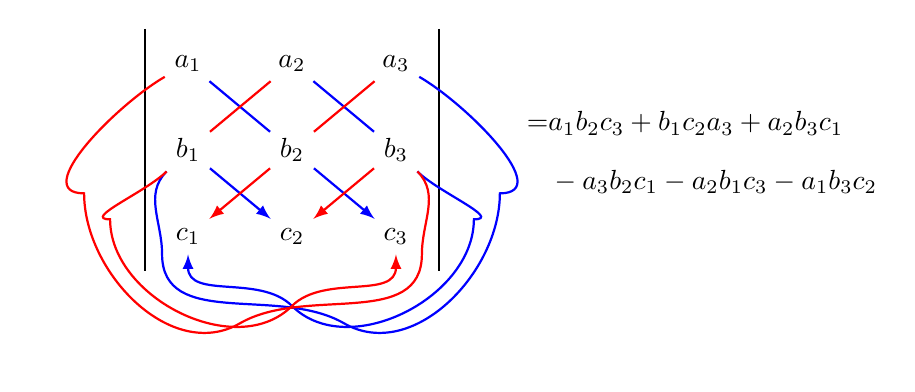
\begin{tikzpicture}[scale=1.1, >=latex]
  % 行列式元素
  \node (a1) at (0, 2) {$a_1$};
  \node (a2) at (1.2, 2) {$a_2$};
  \node (a3) at (2.4, 2) {$a_3$};
  
  \node (b1) at (0, 1) {$b_1$};
  \node (b2) at (1.2, 1) {$b_2$};
  \node (b3) at (2.4, 1) {$b_3$};
  
  \node (c1) at (0, 0) {$c_1$};
  \node (c2) at (1.2, 0) {$c_2$};
  \node (c3) at (2.4, 0) {$c_3$};
  
  % 兩側豎線
  \draw[thick] (-0.5, 2.4) -- (-0.5, -0.4);
  \draw[thick] (2.9, 2.4) -- (2.9, -0.4);
  
  % 向右下（正號項）實線箭頭
  % 1. a1 -> b2 -> c3
  \draw[->, thick, blue] (a1) -- (b2) -- (c3);
  % 2. a2 -> b3 -> 循環繞到底部至 c1
  \draw[thick, blue] (a2) -- (b3);
  \draw[->, thick, blue] (b3) to[out=-45, in=0] (3.3, 0.2) to[out=-90, in=-45] (1.2, -0.8) to[out=135, in=-90] (c1);
  % 3. a3 -> 循環穿過 b1 -> c2
  \draw[thick, blue] (a3) to[out=-30, in=0] (3.6, 0.5) to[out=-90, in=-30] (1.8, -1.0) to[out=150, in=-90] (-0.3, -0.2) to[out=90, in=-135] (b1);
  \draw[->, thick, blue] (b1) -- (c2);
  
  % 向左下（負號項）虛線/紅色箭頭
  % 1. a3 -> b2 -> c1
  \draw[->, thick, red] (a3) -- (b2) -- (c1);
  % 2. a2 -> b1 -> 循環繞至 c3
  \draw[thick, red] (a2) -- (b1);
  \draw[->, thick, red] (b1) to[out=-135, in=180] (-0.9, 0.2) to[out=-90, in=225] (1.2, -0.8) to[out=45, in=-90] (c3);
  % 3. a1 -> 循環穿過 b3 -> c2
  \draw[thick, red] (a1) to[out=-150, in=180] (-1.2, 0.5) to[out=-90, in=210] (0.6, -1.0) to[out=30, in=-90] (2.7, -0.2) to[out=90, in=-45] (b3);
  \draw[->, thick, red] (b3) -- (c2);
  
  % 右側展開式
  \node[right] at (3.8, 1.0) {$\begin{aligned}
    = &a_1 b_2 c_3 + b_1 c_2 a_3 + a_2 b_3 c_1 \\
      &- a_3 b_2 c_1 - a_2 b_1 c_3 - a_1 b_3 c_2
  \end{aligned}$};
\end{tikzpicture}
\caption{三階行列式展開之循環記憶法}\label{fig:det3_sarrus}
\end{figure}

同樣的，向右的箭頭所成的項都冠以正號，向左的箭頭所成的項都冠以負號。

關於三元或更多元一次聯立方程式的進一步討論，將留待以後再述。

\begin{example}\label{ex:4-4-5}
解聯立方程式
\begin{equation*}
\begin{cases}
  2x+y = 0 \\
  -x+3y+z = 2 \\
  4x+3y-z = 1
\end{cases}
\end{equation*}
\end{example}

\begin{solution*}
因為
\begin{equation*}
  \begin{vmatrix}
    2 & 1 & 0 \\
    -1 & 3 & 1 \\
    4 & 3 & -1
  \end{vmatrix}
  = -6 + 4 - 1 - 6 = -9 \neq 0
\end{equation*}
所以這組聯立方程式有唯一的一組解。
\begin{align*}
  x &= \frac{\begin{vmatrix} 0 & 1 & 0 \\ 2 & 3 & 1 \\ 1 & 3 & -1 \end{vmatrix}}{-9} = \frac{3}{-9} = -\frac{1}{3} \text{，}\footnote{原書等式中間誤印為 $\frac{-3}{9} = -\frac{1}{3}$，分子符號錯置，但最終數值正確，詳見\hyperref[sec:master_errata_notes]{目錄前勘誤表}。} \\
  y &= \frac{\begin{vmatrix} 2 & 0 & 0 \\ -1 & 2 & 1 \\ 4 & 1 & -1 \end{vmatrix}}{-9} = \frac{-6}{-9} = \frac{2}{3} \text{，} \\
  z &= \frac{\begin{vmatrix} 2 & 1 & 0 \\ -1 & 3 & 2 \\ 4 & 3 & 1 \end{vmatrix}}{-9} = \frac{3}{-9} = -\frac{1}{3} \text{。}
\end{align*}
\end{solution*}

\subsection*{習題 4-7}\label{sec:ex4-7}
\addcontentsline{toc}{subsection}{習題 4-7}

\begin{enumerate}[1.]
  \item 解下列三元方程式：
  \begin{enumerate}[(i)]
    \item 
    $\begin{cases}
      2x-3y-z = 4 \\
      x+y-z = 2 \\
      4x-y+3z = 1
    \end{cases}$
    \item 
    $\begin{cases}
      2x+3y-5z = 3 \\
      x-2y+z = 0 \\
      3x+y+3z = 7
    \end{cases}$
    \item 
    $\begin{cases}
      2x+4y-3z = 3 \\
      3x-8y+6z = 1 \\
      8x-2y-9z = 4
    \end{cases}$
    \item 
    $\begin{cases}
      x+y+z = l+m+n \\
      lx+my+nz = mn+ln+lm \quad (l, m, n \text{ 不等}) \\
      (m-n)x + (n-l)y + (l-m)z = 0
    \end{cases}$
    \item 
    $\begin{cases}
      \dfrac{6}{x} + \dfrac{2}{y} - \dfrac{5}{z} = 13 \\[1em]
      \dfrac{3}{x} + \dfrac{3}{y} - \dfrac{2}{z} = 13 \\[1em]
      \dfrac{7}{x} + \dfrac{5}{y} - \dfrac{3}{z} = 26
    \end{cases}$
    \item 
    $\begin{cases}
      \dfrac{v+w}{4} = \dfrac{w+u}{3} \\[1em]
      \dfrac{v+w}{4} = \dfrac{u+v}{2} \\[1em]
      u+v+w = 27
    \end{cases}$
    \item 
    $\begin{cases}
      3x-2y = 5 \\
      4x-3y+2z = 11 \\
      x-2y-5z = -7
    \end{cases}$
    \item 
    $\begin{cases}
      5x+3y-6z = 4 \\
      3x-y+2z = 8 \\
      x-2y-2z = 2
    \end{cases}$
  \end{enumerate}

  \item 試證下列各式：
  \begin{enumerate}[(i)]
    \item $\begin{vmatrix} a_1 & a_2 & a_3 \\ b_1 & b_2 & b_3 \\ c_1 & c_2 & c_3 \end{vmatrix} = \begin{vmatrix} a_1 & b_1 & c_1 \\ a_2 & b_2 & c_2 \\ a_3 & b_3 & c_3 \end{vmatrix}$
    \item $\begin{vmatrix} a_1 & b_1 & c_1 \\ a_1 & b_1 & c_1 \\ a_3 & b_3 & c_3 \end{vmatrix} = 0$
    \item $\begin{vmatrix} a_1 & a_2 & a_3 \\ b_1 & b_2 & b_3 \\ c_1 & c_2 & c_3 \end{vmatrix} = - \begin{vmatrix} b_1 & b_2 & b_3 \\ a_1 & a_2 & a_3 \\ c_1 & c_2 & c_3 \end{vmatrix}$
    \item $\begin{vmatrix} a_1 & a_2 & a_3 \\ b_1 & b_2 & b_3 \\ kc_1 & kc_2 & kc_3 \end{vmatrix} = k \begin{vmatrix} a_1 & a_2 & a_3 \\ b_1 & b_2 & b_3 \\ c_1 & c_2 & c_3 \end{vmatrix}$
    \item $\begin{vmatrix} a_1 & a_2 & a_3 \\ b_1 & b_2 & b_3 \\ c_1 & c_2 & c_3 \end{vmatrix} = \begin{vmatrix} a_1 & a_2 & a_3 \\ b_1-ka_1 & b_2-ka_2 & b_3-ka_3 \\ c_1-ma_1 & c_2-ma_2 & c_3-ma_3 \end{vmatrix}$
  \end{enumerate}

  \item 試計算下列各式：
  \begin{multicols}{2}
  \begin{enumerate}[(i)]
    \item $\begin{vmatrix} 3 & 7 & 5 \\ 6 & -9 & 4 \\ -3 & 2 & 7 \end{vmatrix}$
    \item $\begin{vmatrix} 2 & 3 & 4 \\ 7 & -\dfrac{1}{5} & \dfrac{1}{2} \\ 6 & -\dfrac{9}{7} & 9 \end{vmatrix}$
    \item $\begin{vmatrix} 4 & 8 & 9 \\ -8 & -16 & -18 \\ 3 & -5 & 1 \end{vmatrix}$
    \item $\begin{vmatrix} 3 & 12 & 3 \\ \dfrac{1}{9} & 5 & 8 \\ 16 & 15 & 4 \end{vmatrix}$
  \end{enumerate}
  \end{multicols}

  \item 設 $a \in \mathbb{R}$。若方程組
  \begin{equation*}
  \begin{cases}
    3x+y-2z = ax \\
    2x+2y-3z = az \\
    2x-5y+2z = ay
  \end{cases}
  \end{equation*}
  有異於 $(0,0,0)$ 之解，則 $a$ 為多少？\footnote{原書第二、三式右端順序為 $az$ 與 $ay$，此處忠實依原書文字收錄。}

  \item 設 $9x-4y+3z = -7x+2y+15z = 13x-8y-z$ 且 $xyz \neq 0$，求
  \begin{equation*}
    \frac{3x^2-2y^2+z^2-5xy}{4x^2-5y^2-6z^2+2xz} \text{ 之值。}
  \end{equation*}
  （提示：仿例 2，利用例 1 之結論）。
\end{enumerate}
 % 第四章 一次方程式
% =========================================================================
% 《高中數學實驗教材》第一冊（高一上） 
% 第五章 多項式及其運算
% =========================================================================

\section{多項式及其運算}\label{sec:ch5}

在上一章中，我們引入一些符號如 $x, y, z$ 等，用以表示我們在「某一給定問題」中所要求解的未知數，我們也就叫這些符號為\textbf{未知數}。利用這些符號，我們可以把給定問題中，量與量之間的關係用算式表出，這也就是由該問題所產生的方程式。在第四章裏，我們以方程式中最簡單的一次方程式為例，闡述從方程式去解出未知數的基本原理。

一個「未知數」$x$（或 $y$，或 $z$，……等）雖然在未解出之前不知道「它所代表的數等於多少？」但是只要它所代表的是一個數，它在運算上就具有那些任何數皆具有的通性，如分配律、結合律、交換律等等。

所以從運算上著眼，一個未知數 $x$ 就是一個在運算上具有數的通性的符號！同學們可以預想到，對於由一個在運算上具有數的通性的符號（亦即本章 \S 5-1 所定義的不定元）所組成的算式的有系統討論，將是對高次方程式探討的重要基礎！這也就是本章的課題——多項式及其運算。

\subsection{不定元與多項式}\label{sec:5-1}

\subsubsection*{甲、不定元的概念}\label{subsec:5-1-a}

一個不定元就是一個符號（如 $x$，$y$ 或 $z$）。它在運算上具有和數一樣的通性。所以，前面所講到的基本性質，如結合律、交換律、分配律等，在不定元的運算時都可以適用。譬如
\begin{enumerate}[(i)]
  \item $x$ 是一個不定元，則
  \begin{equation*}
    (x \cdot x) \cdot x = x \cdot (x \cdot x) \quad \text{〔結合律〕}
  \end{equation*}
  亦即三個 $x$ 相乘時和括號的括法無關，故可用 $x^3$ 表示之。同理
  \begin{align*}
    (x \cdot x) \cdot (x \cdot x) &= x \cdot (x \cdot (x \cdot x)) = ((x \cdot x) \cdot x) \cdot x \\
    &= x^3 \cdot x = x^4,
  \end{align*}
  依此類推，
  \begin{equation*}
    x^n = \overbrace{x \cdot x \cdot \cdots \cdot x}^{n\text{ 個}}.
  \end{equation*}
  由上述指數的意義，則下述指數定律則仍是結合律的直接結論。
  \begin{equation}\label{eq:exp_rule_1}
    x^n \cdot x^m = x^{n+m} \dots\dots\dots
  \end{equation}

  \item 設 $x, y, z$ 是三個不定元，用結合律和交換律我們可以同樣的把上述「指數定律」推廣為下述形式：
  \begin{equation}\label{eq:exp_rule_multivar}
    (x^l \cdot y^m \cdot z^n) \cdot (x^p \cdot y^q \cdot z^r) = x^{l+p} \cdot y^{m+q} \cdot z^{n+r}.
  \end{equation}

  \item 設 $x, y, z$ 是三個不定元；$a, b$ 是兩個數。則「$a$ 和 $l$ 個 $x$，$m$ 個 $y$，$n$ 個 $z$ 相乘」，其結果是和相乘時的次序與括號的括法無關。故簡潔地可以用符號 $a x^l y^m z^n$ 表示之。譬如\footnote{原書此處掃描檔有歷史墨跡塗抹「$a$ 是個數」字樣，正文中已予剔除還原，見\hyperref[sec:master_errata_notes]{目錄前勘誤表}。}
  \begin{align*}
    2xy &= (2 \cdot x) \cdot y = y \cdot (2 \cdot x) = (y \cdot 2) \cdot x = (y \cdot x) \cdot 2 \\
    &= y \cdot (x \cdot 2). \\
    5x^3 y^2 &= (5 \cdot (x^3 \cdot y^2)) = 5 \cdot ((x \cdot y) \cdot (x^2 \cdot y)) \\
    &= ((y^2 \cdot 5) \cdot x) \cdot (x \cdot x) = (y \cdot 5 \cdot x^2) \cdot (y \cdot x). \\
    7x y^2 z^3 &= (7z^2) \cdot (x y^2 z) = (yz)((7xy) \cdot z^2) \\
    &= (y^2 z) \cdot (7xz^2).
  \end{align*}
  一個可以寫成 $a x^l y^m z^n$ 形式的式子叫做\textbf{單項式}，$a$ 叫做該單項式的\textbf{係數}，$l+m+n$ 叫做該單項式對於 $x, y, z$ 的\textbf{次數}，或簡稱為該單項式的次數。$l$ 叫做該單項式對於 $x$ 的次數，$m$ 叫做該單項式對於 $y$ 的次數，$m+n$ 叫做該單項式對於 $y, z$ 的次數，做此類推。

  \item 為了符合數的通性，我們規定
  \begin{equation*}
    (-a) x^l y^m z^n = -a x^l y^m z^n.
  \end{equation*}
  譬如：
  \begin{align*}
    (-1)x &= -x, \\
    -5x^3 y^4 z^2 &= (-5) x^3 y^4 z^2 = (-5x^3) y^4 z^2.
  \end{align*}
  同樣的，由結合律、分配律，我們不難看出兩個單項式的乘積可以計算如下：
  \begin{equation}\label{eq:mono_prod}
    a x^l y^m z^n \cdot b x^p y^q z^r = a \cdot b \cdot x^{l+p} \cdot y^{m+q} \cdot z^{n+r} \dots\dots\dots
  \end{equation}
  亦即兩個單項式相乘時，其係數相乘，指數相加。所得乘積的次數就等於原來兩個單項式次數的和。
\end{enumerate}

\paragraph{注意：}
我們規定
\begin{equation*}
  x^0 = y^0 = z^0 = 1,
\end{equation*}
則
\begin{align*}
  a &= a \cdot x^0 = a \cdot x^0 \cdot y^0 = a \cdot x^0 \cdot y^0 \cdot z^0, \\
  a x^3 &= a x^3 \cdot y^0 = a x^3 \cdot y^0 \cdot z^0, \\
  a x y^2 &= a x \cdot y^2 \cdot z^0 \text{ 等。}
\end{align*}
所以一個數 $a$，也就可以看成單項式的特例。對於 $x^0, y^0, z^0$ 採取上述規定的好處是：如此定義後，\eqref{eq:mono_prod} 式在 $l, m, n; p, q, r$ 中有些為零時也成立。這也就是我們採取上述規定的理由。

\begin{example}\label{ex:5-1-1}
$1, -2, 8$ 等是 $0$ 次單項式，\\
$x, 3y, -z$ 等都是 $1$ 次單項式，\\
$x^2, 2xy, -3yz$ 等都是 $2$ 次單項式，\\
$\dots\dots\dots\dots\dots\dots\dots\dots\dots\dots$\\
$x^6, 2x y^3 z^2, -8 y^2 z^4$ 等都是 $6$ 次單項式。
\end{example}

\subsubsection*{乙、多項式}\label{subsec:5-1-b}

當我們把不定元和數相乘時，即得種種單項式，如
\begin{equation*}
  -5x^3, \; \frac{1}{2}x^5, \; -\frac{5}{37}x^2 y, \; xyz, \; 10x^{10} y^{10} z^{10}, \text{ 等等。}
\end{equation*}
假如我們把不定元和數以加和乘這兩種運算作種種組合，究竟能得到什麼樣的式子呢？先讓我們來看幾個例子：

\begin{example}\label{ex:5-1-2}
我們把幾個單項式相加，如
\begin{equation}\label{eq:poly_demo_1}
  2x + (-3)x^3 + (-7)x^5 + \frac{1}{7}x^2 + \frac{1}{5}x + 2x^5 \dots\dots\dots
\end{equation}
\begin{equation}\label{eq:poly_demo_2}
  -x^3 y + 2x^3 y^2 + 3xyz - 5xy^2 + 4x^3 y + 5xyz - 6xy^3 + 7z^2 \dots\dots\dots
\end{equation}
\end{example}

這一類的式子，就叫做\textbf{多項式}。（注意：我們把單項式看成是多項式的特例！）只含有一個不定元的多項式通常叫做\textbf{單元多項式}，如 \eqref{eq:poly_demo_1} 式；含有一個以上不定元的多項式叫做\textbf{多元多項式}，如 \eqref{eq:poly_demo_2} 式。由加法交換律可知一個多項式中的各項單項式的次序可以任意交換。平常以「降次」或「升次」\footnote{有些課本用「冪」代「次」，譬如「降冪」、「升冪」等，我們認為「冪」字筆劃較多又不太常見，不如「次」字簡單明瞭。}排列較為方便。例如把 \eqref{eq:poly_demo_1} 重寫為
\begin{equation*}
  (-7x^5 + 2x^5) + (-3)x^3 + \frac{1}{7}x^2 + \left(2x + \frac{1}{5}x\right) \dots\dots\dots \text{降次排列}
\end{equation*}
或
\begin{equation*}
  \left(2x + \frac{1}{5}x\right) + \frac{1}{7}x^2 + (-3)x^3 + (-7x^5 + 2x^5) \dots\dots\dots \text{升次排列}
\end{equation*}
再由分配律，有
\begin{align*}
  -7x^5 + 2x^5 &= (-7+2) \cdot x^5 = -5x^5, \\
  2x + \frac{1}{5}x &= \left(2 + \frac{1}{5}\right)x = \frac{11}{5}x,
\end{align*}
故 \eqref{eq:poly_demo_1} 式可以化簡為
\begin{equation}\label{eq:poly_demo_1_simp}
  -5x^5 - 3x^3 + \frac{1}{7}x^2 + \frac{11}{5}x \dots\dots\dots
\end{equation}

同樣我們可以把 \eqref{eq:poly_demo_2} 式化簡為
\begin{equation}\label{eq:poly_demo_2_simp}
  3x^3 y + 2x^3 y^2 + 8xyz - 5xy^2 - 6xy^3 + 7z^2 \dots\dots\dots
\end{equation}
再關於 $x$ 集項，依 $x$ 降次排列
\begin{equation*}
  (3y + 2y^2)x^3 + (8yz - 5y^2 - 6y^3)x + 7z^2,
\end{equation*}
也可以關於 $y$ 集項，依 $y$ 升次排列
\begin{equation*}
  7z^2 + (3x^3 + 8xz)y + (2x^3 - 5x)y^2 - 6x y^3.
\end{equation*}

\begin{example}\label{ex:5-1-3}
設 $3x^3 - \frac{1}{2}x^2 + \frac{4}{5}x + 7$ 是另外一個多項式，則它和上述 \eqref{eq:poly_demo_1_simp} 式的和可以求之如下：
\begin{align*}
  &\left(3x^3 - \frac{1}{2}x^2 + \frac{4}{5}x + 7\right) + \left(-5x^5 - 3x^3 + \frac{1}{7}x^2 + \frac{11}{5}x\right) \\
  &= 3x^3 - \frac{1}{2}x^2 + \frac{4}{5}x + 7 - 5x^5 - 3x^3 + \frac{1}{7}x^2 + \frac{11}{5}x \quad \text{〔結合律略去括號〕} \\
  &= -5x^5 + (3x^3 - 3x^3) + \left(-\frac{1}{2}x^2 + \frac{1}{7}x^2\right) \\
  &\quad + \left(\frac{4}{5}x + \frac{11}{5}x\right) + 7 \quad \text{〔用交換律以降次排列〕} \\
  &= -5x^5 + \left(-\frac{1}{2} + \frac{1}{7}\right)x^2 + \left(\frac{4}{5} + \frac{11}{5}\right)x + 7 \quad \text{〔用分配律將對應係數相加〕} \\
  &= -5x^5 - \frac{5}{14}x^2 + 3x + 7.
\end{align*}
\end{example}

從上面的運算，我們發現：
\begin{quote}
計算兩個多項式的和時，我們只要把同類項的對應係數相加即可。
\end{quote}
所以一個較為簡便的寫法是：
\begin{equation*}
\begin{array}{rrrrrr}
  &  & 3x^3 & -\frac{1}{2}x^2 & +\frac{4}{5}x & +7 \\
+) & -5x^5 & -3x^3 & +\frac{1}{7}x^2 & +\frac{11}{5}x & \\ \hline
  & -5x^5 & +0x^3 & -\frac{5}{14}x^2 & +3x & +7
\end{array}
\end{equation*}

\begin{example}\label{ex:5-1-4}
現在讓我們來看一看 $x^2+x+1$ 和 $3x^3+x^2-3x-5$ 的乘積是什麼？
\end{example}

\begin{solution*}
\begin{align*}
  &(x^2+x+1) \cdot (3x^3+x^2-3x-5) \\
  &= x^2 \cdot (3x^3+x^2-3x-5) + x \cdot (3x^3+x^2-3x-5) \\
  &\quad + 1 \cdot (3x^3+x^2-3x-5) \quad \text{〔分配律〕} \\
  &= (3x^5+x^4-3x^3-5x^2) + (3x^4+x^3-3x^2-5x) \\
  &\quad + (3x^3+x^2-3x-5) \quad \text{〔分配律；單項式的乘法〕} \\
  &= 3x^5 + (1+3)x^4 + (-3+1+3)x^3 + (-5-3+1)x^2 \\
  &\quad + (-5-3)x - 5 \quad \text{〔多項式的加法〕} \\
  &= 3x^5 + 4x^4 + x^3 - 7x^2 - 8x - 5.
\end{align*}

由上面的例子，我們看出「兩個多項式的乘積依然是一個多項式」！而它們的乘積可以先用「分配律」展開，再用加法去「求和」即得。其算法也可以用下列直式簡潔地表示：
\begin{equation*}
\begin{array}{rrrrrrr}
  &  &  & 3x^3 & +x^2 & -3x & -5 \\
\times) &  &  &  & x^2 & +x & +1 \\ \hline
  &  &  & 3x^3 & +x^2 & -3x & -5 \quad \longleftarrow 1 \cdot (3x^3+x^2-3x-5) \\
  &  & 3x^4 & +x^3 & -3x^2 & -5x & \quad \longleftarrow x \cdot (3x^3+x^2-3x-5) \\
+) & 3x^5 & +x^4 & -3x^3 & -5x^2 &  & \quad \longleftarrow x^2 \cdot (3x^3+x^2-3x-5) \\ \hline
  & 3x^5 & +4x^4 & +x^3 & -7x^2 & -8x & -5
\end{array}
\end{equation*}

事實上多項式的加減及乘除可用分離係數的方法求算，亦即上例中的 $(3x^3+x^2-3x-5) \cdot (x^2+x+1)$ 可以這樣做：
\begin{equation*}
\begin{array}{rrrrrr}
  &  & 3 & +1 & -3 & -5 \\
  &  & 1 & +1 & +1 &  \\ \hline
  &  & +3 & +1 & -3 & -5 \\
  & +3 & +1 & -3 & -5 &  \\
+3 & +1 & -3 & -5 &  &  \\ \hline
3 & 4 & 1 & -7 & -8 & -5
\end{array}
\end{equation*}
雖然省去了不定元 $x$ 的冪次，所有實質都保留了。
\end{solution*}

綜合上述討論，我們知道兩個單元多項式的「和」與「積」依然是多項式。同理，兩個多元多項式的和與積也依然是多元多項式。其計算的原理與方式和上述單元多項式類似。

\subsection*{習題 5-1}\label{sec:ex5-1}
\addcontentsline{toc}{subsection}{習題 5-1}

\begin{enumerate}[1.]
  \item 試將下列各單元多項式化簡後再依升次排列.
  \begin{enumerate}[(1)]
    \item $3x^6 + 2x^2 - 4x^6 + x^5 - x^3 + x + 8 + 6x^2 - x^6$.
    \item $x^5 - x^4 - x^2 + 6 + x + 3x^4$.
    \item $4x^{100} + x^{99} + 6x^7 - 5x + 8x^{10} + 6x^7 - 7x$.
  \end{enumerate}

  \item 化簡 $x^3 + 7x^2 z - 9xyz + 10xz^2 + 7x^3 + 100x^2 y^2 - 60xyy + 30xyz^2 + 9z^3$\footnote{原書式中印為「$-60xyy$」，未併為 $-60xy^2$，正文依原書文字忠實收錄。}，並寫出按 $x$ 升次的式子以及按 $z$ 降次的式子.

  \item 求下列各組多項式的和：
  \begin{enumerate}[(1)]
    \item $f(x)=x^3+2x^2+x-1$, $g(x)=3x^4+2x^3+2x+4$.
    \item $f(x)=1-x+x^2-x^3+x^4$, $g(x)=1+x+x^2+x^3+x^4$.
    \item $f_1(x)=1-x, f_2(x)=x-x^2, f_3(x)=x^2-x^3, \dots, f_n(x)=x^{n-1}-x^n$.
  \end{enumerate}

  \item 試計算下列各組單元多項式的和與積.
  \begin{enumerate}[(i)]
    \item $x^3+x^2+x+1$ 與 $x-1$.
    \item $-2x^4+x^3-x^2+2x-1$ 與 $2x^4+x^3$.
    \item $x^2-x+1$ 與 $x+1$.
    \item $-5x^3+x^2-1$ 與 $5x^3+x^2-1$.
    \item $x^2-2$ 與 $x^2+2$.
  \end{enumerate}

  \item 試求下列各組多項式的和與積：
  \begin{enumerate}[(1)]
    \item $x^3+y^3+3xy+1$, $2x^2-5xy+6y^2+3x-y+4$.
    \item $x^3+2x^2 y+x^2-y^2$, $y^3-2xy-3x+5$.
    \item $x^5+y^4-3x^3 y+xy^2$, $x^2+2xy-3y+2$.
  \end{enumerate}

  \item 試證下列各式：
  \begin{enumerate}[(1)]
    \item $x^3+y^3=(x+y)(x^2-xy+y^2)$.
    \item $x^3-y^3=(x-y)(x^2+xy+y^2)$.
    \item $(x+y+z)^2=x^2+y^2+z^2+2xy+2yz+2xz$.
  \end{enumerate}
\end{enumerate}

\subsubsection*{丙、不定元與未知數的異同}\label{subsec:5-1-c}

不定元與未知數常常用相同的符號如 $x, y, z$ 等表示。但是它們的涵義是截然不同的！不定元只是一個符號，但是未知數是表示某一問題中所要求解的一個數，它在該問題的討論過程中是有其確切的涵義的！也許同學們要問：「那麼為什麼把兩種意義不同的事物，卻故意的用相同的符號去表示呢？」在數學中，符號的選用是很講究的，絕不會故意讓同學們混淆的。對於不定元和未知數所以採用相同的符號的原因有二：
\begin{enumerate}[(i)]
  \item 不定元和未知數雖然涵義不同，但是它們在運算上具有相同的性質。
  \item 當我們把 $x$ 用在方程式 $[x^2-2x-15=0]$ 時，$x$ 顯然表示滿足該方程式的一個未知數，當我們把 $x$ 用在多項式 $[x^2-2x-15]$ 時，$x$ 就表示一個不定元，所以上述一個符號的兩種用法是很容易由它所用的地方去判定它應該是屬於那一種，而不至於導致混淆。
\end{enumerate}

對於以上的說明，同學們恐怕還有疑問。一個未知數總是一個數，能作運算，有確切涵義，這是好懂的了。一個不定元，一方面能作運算，而卻又不一定是個數，這樣的東西是什麼？有什麼用處？為什麼要討論這樣的東西？事實上，在數學裏可以作運算，在運算上與數十分相似，而不是數的東西很多很多。比如「矩陣」，「函數」（以後都會談到）等等都是。而不定元只不過是這類「可資運算」的東西的「通稱」而已。在我們只集中注意力在運算通性而暫不計較它的實質時，我們就用不定元這個名詞，而只說它是一個「符號」。以後有需要的時候，這個符號可以「賦予」種種實際的意義。這樣的做法，有許多方便的地方。不過對於我們初學的人，對於數以外的東西不曾多見，自然會稍覺奇怪了。

\subsection{單元多項式的加、乘及其基本性質}\label{sec:5-2}

\subsubsection*{甲、多項式的係數與符號}\label{subsec:5-2-a}

在上一節中，我們引入不定元這個概念。並且說明用不定元 $x$ 和數，以加、乘這兩種運算作種種組合，所得者皆為 $x$ 的多項式。但是在上一節中我們並沒有明確地說明所用的「數」是取自那一個數系。譬如下列五個多項式：
\begin{enumerate}[(1)]
  \item $2x-3x^2+5x+7$.
  \item $x^2-2$.
  \item $\frac{1}{3}x^3+\frac{1}{2}x^2+7x-3$.
  \item $x+\sqrt{2}$.
  \item $x-\sqrt{2}$.
\end{enumerate}
(1)、(2) 的係數皆取自整數系 $\mathbb{Z}$，我們稱之謂整係數多項式；(1)、(2)、(3) 的係數皆取自有理數系 $\mathbb{Q}$，我們稱之謂有理係數多項式；(1)、(2)、(3)、(4)、(5) 的係數皆取自實數系 $\mathbb{R}$，我們稱之謂實係數多項式。由此可見一個整係數多項式也是有理係數多項式或實係數多項式，而一個有理多項式也是實數多項式。

\paragraph{符號用法：}
在本書中，我們將採用：
\begin{align*}
  \mathbb{Z}[x] &: \text{表示所有 $x$ 的整係數多項式所成的集合，} \\
  \mathbb{Q}[x] &: \text{表示所有 $x$ 的有理係數多項式所成的集合，} \\
  \mathbb{R}[x] &: \text{表示所有 $x$ 的實係數多項式所成的集合，} \\
  \mathbb{Z}[x,y] &: \text{表示所有 $x, y$ 的整係數多項式所成的集合，} \\
  \mathbb{Q}[x,y] &: \text{表示所有 $x, y$ 的有理係數多項式所成的集合，} \\
  \mathbb{R}[x,y] &: \text{表示所有 $x, y$ 的實係數多項式所成的集合，}
\end{align*}
依此類推。

上述諸集合中，顯然有下列關係：
\begin{align*}
  \mathbb{R}[x] \supseteq \mathbb{Q}[x] \supseteq \mathbb{Z}[x], \quad &\text{〔因為 $\mathbb{R} \supseteq \mathbb{Q} \supseteq \mathbb{Z}$〕} \\
  \mathbb{Z}[x,y] \supseteq \mathbb{Z}[x] \supseteq \mathbb{Z} \\
  \mathbb{Q}[x,y] \supseteq \mathbb{Q}[x] \supseteq \mathbb{Q} \\
  \mathbb{R}[x,y] \supseteq \mathbb{R}[x] \supseteq \mathbb{R}
\end{align*}
〔因為一個 $x$ 的多項式也可以看成 $x, y$ 的多項式；只是它每項關於 $y$ 的次數皆為零；不等於 $0$ 的數可以看成零次多項式，而且我們把 $0$ 看成係數全是 $0$ 的多項式。〕

正如我們在第三章的討論中用 $a, b, c$ 等符號表示某一數系中的一般元素，我們將用 $f(x)$, $g(x)$, $q(x)$, $r(x)$ 等表示 $\mathbb{R}[x]$（或 $\mathbb{Q}[x]$，或 $\mathbb{Z}[x]$）中的一般元素，用 $f(x,y)$, $g(x,y)$, $q(x,y)$, $r(x,y)$ 等表示 $\mathbb{R}[x,y]$（或 $\mathbb{Q}[x,y]$，或 $\mathbb{Z}[x,y]$）中的一般元素。例如 $f(x)$ 是 $\mathbb{Q}[x]$ 中的一個一般元素，則 $f(x)$ 可以寫成下述形式：
\begin{equation}\label{eq:poly_general_form}
  f(x) = a_n x^n + a_{n-1} x^{n-1} + a_{n-2} x^{n-2} + \dots + a_1 x + a_0 \dots\dots\dots
\end{equation}
其中 $n$ 為一適當的非負整數，$a_n, a_{n-1}, a_{n-2}, \dots, a_1, a_0 \in \mathbb{Q}$。當然上述符號中的 $a_n, \dots, a_1, a_0$ 中有些可以是零。譬如 $x^5+x^2-4$ 就是 $n=5, a_5=1, a_4=0, a_3=0, a_2=1, a_1=0, a_0=-4$ 時，\eqref{eq:poly_general_form} 式所表示者。上述符號 $a_i$ 中右下角的 $i$ 叫做\textbf{足標}\footnote{寫在右下角的表示足標，寫在右上角的表示次，又一般的多項式的次數 $n$ 可以很大，譬如 $n=36000$，如不用足標則我們得要 $36000$ 個字母才夠，是不是？}，我們用它來表示 $x^i$ 的係數，同學們只要在開始時小心些，用慣了是一種又簡明又方便的符號。再者，如果係數不是全等於 $0$，我們可以假設首項係數 $a_n \neq 0$；否則我們可以把 $a_n x^n$ 略去。

\begin{example}\label{ex:5-2-1}
$0 \in \mathbb{Z}$ 所以 $0$ 屬於 $\mathbb{Z}[x], \mathbb{Q}[x], \mathbb{R}[x], \mathbb{Z}[x,y], \mathbb{Q}[x,y], \mathbb{R}[x,y]$
\end{example}

\begin{example}\label{ex:5-2-2}
$x+\frac{1}{2}y \in \mathbb{Q}[x,y]$，但 $x+\frac{1}{2}y \notin \mathbb{Z}[x,y], \mathbb{Q}[x], \mathbb{Q}[y]$。
\end{example}

\begin{example}\label{ex:5-2-3}
$\sqrt{2}x \in \mathbb{R}[x], \mathbb{R}[x,y]$；但 $\sqrt{2}x \notin \mathbb{Z}[x], \mathbb{Q}[x], \mathbb{Z}[x,y], \mathbb{Q}[x,y]$。
\end{example}

\begin{example}\label{ex:5-2-4}
$\mathbb{Q}[x] \cap \mathbb{Q}[y] = \mathbb{Q}$。
\end{example}

\subsection*{習題 5-2}\label{sec:ex5-2}
\addcontentsline{toc}{subsection}{習題 5-2}

\begin{enumerate}[1.]
  \item 下列多項式各屬於 $\mathbb{Z}[x], \mathbb{Q}[x], \mathbb{R}[x]$ 中那些集合？
  \begin{enumerate}[(i)]
    \item $f(x)=\sqrt{2}$.
    \item $g(x)=2x^2+\frac{7}{3}x+\frac{3}{4}$.
    \item $h(x)=x^3-5$.
    \item $\varphi(x)=x^3+\sqrt{2}x^2+\sqrt{2}x+1$.
    \item $\psi(x)=x+\frac{1}{2}$.
    \item $F(x)=\sqrt{3}+2x$.
  \end{enumerate}

  \item 下列諸多項式各屬於 $\mathbb{Z}[x,y], \mathbb{Q}[x,y], \mathbb{R}[x,y]$ 中那些集合？
  \begin{enumerate}[(i)]
    \item $f(x)=3x^2+5xy+\frac{1}{2}y^2$.
    \item $g(x)=\sqrt{2}x^4 y+3x^2 y^2+\sqrt{5}xy^2-7xy^5$.
    \item $h(x)=6x^5-5x^4 y-3x^2 y^3+y^5$.
    \item $\varphi(x)=\frac{1}{2}x^3+\frac{3}{5}xy^2-\sqrt{5}y^3$.
    \item $\psi(x)=5x+2y+6$.
  \end{enumerate}

  \item 寫出 $\mathbb{Z}[x,y], \mathbb{Q}[x,y], \mathbb{R}[x,y]$ 三個集合的包含關係.

  \item 求下列各交集：
  \begin{multicols}{2}
  \begin{enumerate}[(i)]
    \item $\mathbb{Z}[x,y] \cap \mathbb{Z}[x]$
    \item $\mathbb{Z}[x] \cap \mathbb{R}$
    \item $\mathbb{R}[x,y] \cap \mathbb{Q}[x]$
    \item $\mathbb{Z}[x,y] \cap \mathbb{R}[x]$
    \item $\mathbb{Q}[x,y] \cap \mathbb{R}$
    \item $\mathbb{Q}[x] \cap \mathbb{Q}[y]$
  \end{enumerate}
  \end{multicols}

  \item $f(x,y) \in \mathbb{Q}[x,y]$，表示 $f(x,y)$ 是 $\mathbb{Q}[x,y]$ 中的一個典型元素，請寫出它的一般形式.
\end{enumerate}

\subsubsection*{乙、多項式基本運算}\label{subsec:5-2-b}

為了討論多項式運算的通性，我們再將多項式加法與乘法，給一個正式的定義。由於這些定義在 $\mathbb{Z}[x], \mathbb{Q}[x], \mathbb{R}[x]$ 中皆一樣，我們僅需以 $\mathbb{Q}[x]$ 為例，說明如下：

\begin{definition*}
設 $f(x), g(x) \in \mathbb{Q}[x]$ 為兩個有理係數多項式，
\begin{align*}
  f(x) &= a_n x^n + a_{n-1} x^{n-1} + \dots + a_1 x + a_0, \quad a_n \neq 0, \\
  g(x) &= b_m x^m + b_{m-1} x^{m-1} + \dots + b_1 x + b_0, \quad b_m \neq 0.
\end{align*}
則
\begin{enumerate}[(i)]
  \item 兩多項式相等的意思，就是他們的各項係數皆相等。換句話說
  \begin{equation*}
    f(x)=g(x) \iff m=n, \text{ 且 } a_n=b_m, a_{n-1}=b_{m-1}, \dots, a_0=b_0.
  \end{equation*}

  \item 設 $m \le n$，則 $f(x)$ 與 $g(x)$ 的\textbf{和}，定義為
  \begin{align*}
    f(x)+g(x) &= a_n x^n + \dots + (a_m+b_m)x^m + (a_{m-1}+b_{m-1})x^{m-1} \\
    &\quad + \dots + (a_1+b_1)x + (a_0+b_0).
  \end{align*}
  （亦即兩個多項式 $f(x), g(x)$ 相加時，其對應項的係數相加。）因此，$f(x)+g(x) \in \mathbb{Q}[x]$。

  \item $f(x)$ 與 $g(x)$ 的「\textbf{積}」，定義為
  \begin{align*}
    f(x) \cdot g(x) &= (a_n x^n + a_{n-1} x^{n-1} + \dots + a_0) \cdot (b_m x^m + b_{m-1} x^{m-1} + \dots + b_0) \\
    &= a_n b_m x^{n+m} + (a_n b_{m-1} + a_{n-1} b_m) x^{n+m-1} + \dots \\
    &\quad + (a_2 b_0 + a_1 b_1 + a_0 b_2) x^2 + (a_1 b_0 + a_0 b_1) x + a_0 b_0.
  \end{align*}
  （亦即 $f(x)$ 和 $g(x)$ 的積可由分配律展開後集項而得，其 $x^k$ 的係數是所有 $a_i b_j$，而 $i+j=k$ 的諸項之和，通常以符號 $\sum_{i+j=k} a_i b_j$ 表之）\footnote{上述的定義只是把同學們在國中所學的多項式的加法與乘法用一般性的符號表達出來，以供在驗證多項式通性時之用。在實例的計算時，仍以直接用直式計算來得方便。\\
  其中 $\sum$ 表示“和”的意思，通常以 $\sum_{i=1}^n a_i$ 表 $a_1+a_2+\dots+a_n$。}因此，$f(x) \cdot g(x) \in \mathbb{Q}[x]$。
\end{enumerate}
\end{definition*}

由上述定義，我們不難驗證下列基本性質：
\begin{enumerate}[(I)]
  \item 
  \begin{align*}
    f(x)+g(x) &= g(x)+f(x), \\
    f(x) \cdot g(x) &= g(x) \cdot f(x). \quad \text{〔交換律〕}
  \end{align*}

  \item 
  \begin{align*}
    (f(x)+g(x))+h(x) &= f(x)+(g(x)+h(x)), \\
    (f(x) \cdot g(x)) \cdot h(x) &= f(x) \cdot (g(x) \cdot h(x)). \quad \text{〔結合律〕}
  \end{align*}

  \item 
  \begin{align*}
    f(x)+0 &= 0+f(x) = f(x), \\
    f(x) \cdot 0 &= 0 \cdot f(x) = 0. \quad \text{〔0 之特性〕}
  \end{align*}

  \item 
  \begin{equation*}
    1 \cdot f(x) = f(x) \cdot 1 = f(x). \quad \text{〔1 之特性〕}
  \end{equation*}

  \item 
  \begin{equation*}
    f(x) \cdot (g(x)+h(x)) = f(x) \cdot g(x) + f(x) \cdot h(x). \quad \text{〔分配律〕}
  \end{equation*}
\end{enumerate}

\begin{definition*}
當 $f(x)=a_n x^n + a_{n-1} x^{n-1} + \dots + a_0$，而 $a_n \neq 0$ 時，我們定義 $f(x)$ 的\textbf{次數}為 $n$，以 $\deg f(x)$ 記之。
\end{definition*}

\paragraph{注意：}
根據上節，一個常數也可以看做是一個多項式，因此「$0$」也是多項式。在需要強調時，我們也稱 $0$ 為\textbf{零多項式}，但需注意在上述的定義中，我們沒有規定零多項式的次數。而在另一方面，一個不等於 $0$ 的常數，是一個次數為 $0$ 的多項式。

\begin{enumerate}[label=(\Roman*), start=6]
  \item 若 $f(x) \neq 0$ 且 $g(x) \neq 0$，則 $f(x) \cdot g(x) \neq 0$ 並且
  \begin{equation*}
    \deg(f(x) \cdot g(x)) = \deg f(x) + \deg g(x).
  \end{equation*}
  換言之：$f(x) \cdot g(x) = 0 \implies f(x)=0$ 或 $g(x)=0$。
\end{enumerate}

\paragraph{注意：}
在 (VI) 中，$f(x) \neq 0$ 是指「$f(x)$ 不是零多項式」的意思，根據多項式相等的定義，這也就是說 $f(x)$ 至少含有一個係數不為 $0$ 的項。

同樣的，(VI) 中的 $f(x)=0$ 是指「$f(x)$ 等於零多項式的意思」，也就是說 $f(x)$ 的各項係數皆為零。

\begin{example}\label{ex:5-2-5}
$f(x)=0, g(x)=2x+3$，
\begin{align*}
  f(x)+g(x) &= 2x+3 = g(x). \\
  f(x) \cdot g(x) &= 0.
\end{align*}
\end{example}

\begin{example}\label{ex:5-2-6}
$f(x)=1, g(x)=x^2+1$，
\begin{align*}
  f(x)+g(x) &= x^2+2. \\
  f(x) \cdot g(x) &= x^2+1 = g(x).
\end{align*}
\end{example}

\begin{example}\label{ex:5-2-7}
$f(x)=x^2+1, g(x)=2x^3+x+3$，
\begin{align*}
  f(x)+g(x) &= 2x^3+x^2+x+4. \\
  f(x) \cdot g(x) &= 2x^5+3x^3+3x^2+x+3.
\end{align*}
$\deg f(x)=2, \deg g(x)=3$，
\begin{align*}
  \deg[f(x)+g(x)] &= 3 = \deg g(x). \\
  \deg[f(x) \cdot g(x)] &= 5 = \deg f(x) + \deg g(x).
\end{align*}
\end{example}

\subsection*{習題 5-3}\label{sec:ex5-3}
\addcontentsline{toc}{subsection}{習題 5-3}

\begin{enumerate}[1.]
  \item 展開再整理下列各多項式.
  \begin{enumerate}[(1)]
    \item $(x-y)(x-z)$.
    \item $(2x-3y)^2(x+z)$.
    \item $(x-y)^3$.
    \item $(1-x)(1+x+x^2+\dots+x^{n-1})$.
    \item $(x+y)^3$.\label{item:ex5-3-1-5}
    \item $(x+y)(x^{n-1}-x^{n-2}y+x^{n-3}y^2-\dots-y^{n-1})$，$n$ 為偶數。
    \item $(x+y)(x^{n-1}-x^{n-2}y+x^{n-3}y^2-\dots+y^{n-1})$，$n$ 為奇數。
  \end{enumerate}

  \item 設 $f(x), g(x) \in \mathbb{Z}[x]$，試證 $f(x)+g(x), f(x)g(x) \in \mathbb{Z}[x]$。

  \item 證明多項式的加法交換律，加法結合律，乘法交換律，乘法結合律及分配律。

  \item 試證性質 (VI) 中：
  \begin{equation*}
    \deg[f(x) \cdot g(x)] = \deg f(x) + \deg g(x). \quad (f(x) \neq 0, g(x) \neq 0).
  \end{equation*}

  \item 假設 $f(x), g(x), f(x)+g(x)$，都不是零，證明
  \begin{equation*}
    \deg(f(x)+g(x)) \le \text{Max}(\deg f(x), \deg g(x)).
  \end{equation*}
  這裏 $\text{Max}(a, b)$ 是指 $a, b$ 中較大的數。
\end{enumerate}

\subsection{變數與函數，多項式函數}\label{sec:5-3}

\subsubsection*{甲、變數與函數}\label{subsec:5-3-a}

在第一章 \S 1-1 討論「數學的題材」時，我們曾以「氣體的體積、溫度、壓力」這些量之間的相互關係為例，說明函數的概念。在該段的討論中，我們初步的定義函數（function）這個基本概念如下：
\begin{quote}
「函數的定義：當某一量 $y$ 隨著另一量 $x$ 的給定而隨之確定時，我們說 $y$ 是 $x$ 的函數，通常以符號 $y=f(x)$ 表示之。」
\end{quote}
也許用心的同學們業已注意到，我們原本用來表示「未知數」或「不定元」的符號如 $x, y, z \dots\dots$ 等，在上述函數符號「$y=f(x)$」中顯然又有另外一種用法了！所以我們首先說明一下 $x, y$ 在函數符號「$y=f(x)$」中確切的涵義。

\begin{example}\label{ex:5-3-1}
今有溫度固定在 $0^\circ\text{C}$ 的氫氣 $2$ 克，設其壓力為 $x$「大氣壓」，其體積為 $y$ 公升，則按波義耳定律，$x$ 與 $y$ 間有下述關係，即
\begin{equation}\label{eq:boyle_demo}
  y = (22.4) \cdot \frac{1}{x} \dots\dots\dots
\end{equation}
\end{example}

在 \eqref{eq:boyle_demo} 式中，$x$ 是用來表示「該氣體」的壓力有多少大氣壓。該氣體的壓力是可以任意變更的，所以 $x$ 是用來表示一個任意的「正實數」。同樣的，$y$ 在 \eqref{eq:boyle_demo} 式中也是用以表示一個任意的「正實數」（即該氣體的體積有多少公升），而 \eqref{eq:boyle_demo} 式所說明的事實是：「$x, y$ 的值都可以在正實數這個範圍內任意變更，但是『$x$ 的值』和『$y$ 的值』之間須具有 \eqref{eq:boyle_demo} 式所示的關係！」這種由 $x$ 的值可以去確定 $y$ 的值的關係（亦即 $y$ 隨 $x$ 而定的關係），數學的術語稱之為「函數」亦即「$y$ 是 $x$ 的函數」。

\begin{example}\label{ex:5-3-2}
寄一封航空信的郵資是由該信的重量而定。亦即「航空信的郵資」是「重量」的函數，如以 $x$ 表示重量（以公分計），以 $y$ 表示郵資（以元計），則從臺灣到歐、美、非的「航空信郵資函數」$y=f(x)$ 如下：
\begin{align*}
  \text{當 } 0 < x \le 10 \text{ 時} \quad & y = 8 \\
  10 < x \le 20 \text{ 時} \quad & y = 8+8 \\
  \dots\dots\dots\dots\dots\dots\dots & \dots\dots\dots\dots\dots \tag{2} \\
  10 \cdot n < x \le 10 \cdot (n+1) \text{ 時} \quad & y = 8+n \cdot 8
\end{align*}
\end{example}

在上述函數中，$x$ 的值可以在「正實數」這個範圍內任意變更。$y$ 的值是一個正整數，它可以由 $x$ 按上述規定計算而得。

\paragraph{注意：}
對於一個函數 $y=f(x)$，$y$ 的值並不一定隨「$x$ 的值變更」而隨之變更。譬如例 2 中 $x$ 在 $10n$ 和 $10 \cdot (n+1)$ 之間變更時，$y$ 的值都是 $8+n \cdot 8$。要記得在函數的定義中，我們說 $y$ 隨著 $x$ 的給定而隨之確定。（我們並不是說 $y$ 隨著 $x$ 的變更而隨之變更。）

由上述剖析，我們確定變數的定義如下：
\begin{definition*}
一個「\textbf{變數}」就是一個符號如 $x, y, z$ 等，用以表示某一範圍的任意一數。（或者說：某一「數集」中的任意一數）故在問題討論的過程中，其所表示之值可以在「該給定範圍」中任意變更。
\end{definition*}

用上述「變數」這種符號後，我們可以把前面的函數的定義重述如下：
\begin{definition*}
設 $x, y$ 為二變數，令 $A, B$ 分別表示 $x$ 與 $y$ 之變動範圍數集，若對每一 $x \in A$，皆有一在 $B$ 中確定之對應數 $y$，則我們說：這一種對應是一個由 $A$ 到 $B$ 的\textbf{函數}，以符號
\begin{equation*}
  f: A \longrightarrow B
\end{equation*}
表示，或寫為 $y=f(x), x \in A$。以 $f(a)$ 表示 $A$ 中元素 $a$ 的對應值。數集 $A$ 叫做函數 $f$ 的\textbf{定義域}。
\end{definition*}

\begin{example}\label{ex:5-3-3}
圓的面積是半徑的函數。設圓的半徑為 $x$，面積為 $y$，則 $y=f(x)=\pi x^2$。
\end{example}

\begin{example}\label{ex:5-3-4}
對於任意實數 $x$，$[x]$ 表示不超過 $x$ 的最大整數。例如
\begin{equation*}
  \left[\frac{5}{2}\right]=2, \quad [3]=3, \quad [\pi]=3, \quad [-1.5]=-2, \quad [0.6]=0.
\end{equation*}
則 $y=f(x)=[x]$ 為一個由 $\mathbb{R}$ 到 $\mathbb{Z}$ 的函數。即 $f: \mathbb{R} \longrightarrow \mathbb{Z}$，$f$ 稱為\textbf{高斯（Gauss）函數}。
\end{example}

利用這個函數可將例 2 中的航空郵資函數表示如下：
\begin{equation*}
  y = f(x) = -8 \left[-\frac{x}{10}\right], \quad x > 0.
\end{equation*}

有許多人常會這樣的問：為何要學數學？學這些與生活無關，又乏味的數學，到頭來得到了什麼？看不見動機，學習數學的趣味自然提不起來，不是嗎？其實數學是用來解決生活上的問題，就我們所知，一些生活上發生的問題大半可以由數學的處理得到簡單而合理的解決，但是，想想如果我們首先未具備相當的數學能力，當一些生活複雜的問題臨頭時，免不了會感到束手無策，難以應付，（你不也常常想到我們常用極原始的方法解決生活問題嗎？）以下我們舉一個較為複雜的例子，從函數的功用，來認識函數。

譬如：某農民有田 $100$ 畝，全種落花生，在正常的天候下，影響收成的因素很多，例如肥料、人工、農藥、技術及品種等。這些影響收成的因素，經數量化後可視為自變數，分別以 $x, y, z, u, v, w$ 表之，收成量稱為應變數，以 $S$ 表之，其相互關係，以符號 $S=f(x, y, z, u, v, w)$ 表之。這個關係式是不是可以從調查很多農家的耕作情形所得的資料及數據表示呢？當然，我們是想要求這樣的函數關係的，但絕不是為了求這函數而求這函數的。想想看，施肥不足，能致使收成量減少，但施肥過量亦能導致收成量減少（參考生物）。我們當然想知道如何適當地控制其因素，使得其收成量為最大，這就是數學能幫助我們解決生活上的問題的一個實例。

\subsection*{習題 5-4}\label{sec:ex5-4}
\addcontentsline{toc}{subsection}{習題 5-4}

\begin{enumerate}[1.]
  \item 設 $A$ 為你的學校高一所有班級的集合，定義 $f: A \longrightarrow \mathbb{N}$ 如下，$x \in A$，$f(x)$ 是 $x$ 班上的學生數目，請你把所有的函數值寫下來。
  \item 西瓜一斤為 $a$ 元，以 $x$ 表斤數，$f(x)$ 表價錢。寫出此函數 $f(x)$ 的式子來。
  \item 設 $f(x)=[x]+\left[x+\frac{1}{3}\right]+\left[x+\frac{2}{3}\right]$，試求 $f(0)+f(1)$。
  \item 試證 $[x-[x]]=0$。
  \item 函數 $f, g: \{x \mid -1 \le x \le 2\} \longrightarrow \mathbb{R}$ 定義如下：
  \begin{align*}
    f: \quad &\text{當 } -1 \le x < \frac{1}{3} \text{ 時} \quad f(x)=2 \\
    &\text{當 } x = \frac{1}{3} \text{ 時} \quad f(x)=-3 \\
    &\text{當 } \frac{1}{3} < x < \frac{1}{2} \text{ 時} \quad f(x)=\frac{1}{2} \\
    &\text{當 } \frac{1}{2} \le x \le 2 \text{ 時} \quad f(x)=0 \\
    g: \quad &\text{當 } -1 \le x \le 0 \text{ 時} \quad g(x)=0 \\
    &\text{當 } 0 < x \le \frac{1}{3} \text{ 時} \quad g(x)=\sqrt{2} \\
    &\text{當 } \frac{1}{3} < x < 2 \text{ 時} \quad g(x)=\frac{1}{3} \\
    &\text{當 } x = 2 \text{ 時} \quad g(x)=4
  \end{align*}
  如果定義函數 $h, k: \{x \mid -1 \le x \le 2\} \longrightarrow \mathbb{R}$ 為 $h(x)=f(x)+g(x)$，$k(x)=f(x) \cdot g(x)$ 請分別寫出 $h(x)$ 和 $k(x)$ 的值來。
  \item 設函數 $f(x)=-[[x]-x]$，試證：$f(\mathbb{R})=\{0, 1\}$。
  \item 用 $x$ 表示計程車行走之距離，用 $y$ 表示車費，那麼 $y$ 是 $x$ 的函數，請用高斯符號表示這個函數，例如民國六十年九月車資標準如下：
  \begin{align*}
    0 < x < 1, \quad & y = 6. \\
    1 \le x < \frac{3}{2}, \quad & y = 6+2.50. \\
    \frac{3}{2} \le x < 2, \quad & y = 6+2 \times 2.50. \\
    \dots\dots\dots\dots & \dots\dots\dots\dots \\
    \frac{n}{2} \le x < \frac{n+1}{2}, \quad & y = 6+(n-1)2.50.
  \end{align*}
\end{enumerate}

\subsubsection*{乙、多項式函數}\label{subsec:5-3-b}

設有一多項式
\begin{equation*}
  f(x) = a_n x^n + a_{n-1} x^{n-1} + \dots + a_0
\end{equation*}
我們已經說過，$f(x)$ 中的 $x$ 是一個不定元，只是一個符號，我們對 $x$ 的唯一要求，是它的運算與數的運算滿足相同的法則，但 $x$ 是否是一個數，則無關緊要。

現在我們任意選定一數 $c \in \mathbb{R}$，則
\begin{equation*}
  a_n c^n + a_{n-1} c^{n-1} + \dots + a_0
\end{equation*}
也是 $\mathbb{R}$ 中一個數，這個數由於 $c$ 的給定而隨之確定。換句話說，我們由多項式 $f(x)$ 而得到一個把 $c$ 對應到 $a_n c^n + a_{n-1} c^{n-1} + \dots + a_0$ 的函數，為方便起見，這個函數仍以 $f$ 表示。所以 $c$ 的對應值
\begin{equation*}
  f(c) = a_n c^n + a_{n-1} c^{n-1} + \dots + a_0.
\end{equation*}
在這個式子中我們把 $c$ 改寫為 $x$，得
\begin{equation*}
  f(x) = a_n x^n + a_{n-1} x^{n-1} + \dots + a_0, \quad x \in \mathbb{R}.
\end{equation*}
這樣一來，$x$ 就不再是一個不定元，而是一個變數了，而原來的多項式也就變成一函數了，叫做\textbf{多項式函數}。我們通常仍以
\begin{equation*}
  y = f(x)
\end{equation*}
表示由多項式 $f(x)$ 所定義的多項式函數。

\begin{example}\label{ex:5-3-5}
$f(x)=x^2$ 是一個多項式，$y=f(x)=x^2$ 是一個多項式函數。它的意思是 $y$ 的值可以由 $x$ 的值的平方而得。譬如
\begin{equation*}
  f(0)=0^2=0, \; f(1)=1^2=1, \; f(2)=2^2=4, \dots\dots \text{等等.}
\end{equation*}
\end{example}

\begin{example}\label{ex:5-3-6}
「$y=x^2$」表示一個函數。即 $y$ 的值可以由 $x$ 的值平方而得。\\
「$y=(x+1)^2$」表示一個函數。即 $y$ 的值可以由 $x$ 的值加 $1$ 後再平方而得。\\
「$y=3x^5-13$」表示一個函數。即 $y$ 的值可以由 $x$ 的值的 $5$ 次方的 $3$ 倍再減 $13$ 而得。
\end{example}

以此類推，對於任何一個給定的多項式
\begin{equation*}
  f(x) = a_n x^n + a_{n-1} x^{n-1} + \dots + a_0,
\end{equation*}
則
\begin{equation*}
  y = f(x) = a_n x^n + a_{n-1} x^{n-1} + \dots + a_0,
\end{equation*}
表示一個函數。這就是上節中所說把不定元賦予意義。更確切的說，多項式 $f(x)$ 中的不定元 $x$ 賦予意義為數時，就得到一個函數。其實上述式子不但說「$y$ 的值」隨「$x$ 的值」而定，而且告訴我們如何用那些給定係數 $a_n, a_{n-1}, \dots, a_0$ 及「加」、「乘」運算去從 $x$ 的值求得對應的 $y$ 值。這一類函數叫做多項式函數。

\subsubsection*{丙、符號用法}\label{subsec:5-3-c}

\begin{enumerate}[(i)]
  \item 未知數，不定元，變數常用 $x, y, z$ 等相同的符號表示，但是其所用的場合是截然不同的。譬如
  \begin{align*}
    &\text{在 } x^2-x-6=0 \text{ 中，$x$ 表示一個未知數；} \\
    &\text{在 } x^2-x-6 \text{ 中，$x$ 表示一個不定元；} \\
    &\text{在 } y=x^2-x-6 \text{ 中，$x$ 表示一個變數。}
  \end{align*}
  所以同學們只要隨時注意，是很容量確定式子中 $x, y, z$ 所表示的究竟是未知數、不定元還是變數。

  \item 對於函數 $y=f(x)$，我們用符號 $f(a)$ 表示當 $x$ 的值為 $a$ 時，所隨之而定 $y$ 的值。亦即當 $x=a$ 時 $y=f(a)$。
\end{enumerate}

\begin{example}\label{ex:5-3-7}
設 $y=f(x)=x^2-x-6$，則
\begin{align*}
  f(0) &= -6, \\
  f(1) &= -6, \\
  f(2) &= -4, \\
  f(3) &= 0, \\
  f(\sqrt{7}) &= (\sqrt{7})^2 - \sqrt{7} - 6 = 1 - \sqrt{7}.
\end{align*}
\end{example}

\begin{example}\label{ex:5-3-8}
設
\begin{equation*}
  f(x) = \begin{cases}
    3x-1 & \text{當 } x > 3 \text{ 時} \\
    x^2-2 & \text{當 } -2 \le x \le 3 \text{ 時} \\
    2x+3 & \text{當 } x < -2 \text{ 時}
  \end{cases}
\end{equation*}
則
\begin{align*}
  f(4) &= 3 \cdot 4 - 1 = 11, \\
  f(2) &= 2^2 - 2 = 2, \\
  f(-5) &= 2 \cdot (-5) + 3 = -7.
\end{align*}
\end{example}

\paragraph{注意：}
由 $f(x)$ 的定義可以看出函數 $f$ 的定義域被分成三段，在每一段中，函數由不同的多項式來表示，因此要求函數在某一點的值時，先要看這一點在那一段中。

\begin{enumerate}[label=(\roman*), start=3]
  \item 在 \S 5-1, \S 5-2 中所敘述的多項式運算中，我們一再說不定元在運算上具有一切數字運算的通性，如結合律、交換律、分配律等。這個事實，有一個重要的結論，就是：在一多項式等式中，將不定元 $x$ 以任何實數「代入」時，仍得一等式。譬如
  \begin{align*}
    f(x)+g(x)=h(x) &\implies \text{對於任意數 $a$，有 } f(a)+g(a)=h(a); \\
    f(x) \cdot g(x)=k(x) &\implies \text{對於任意數 $a$，有 } f(a) \cdot g(a)=k(a).
  \end{align*}
\end{enumerate}

同學們要注意，在上面兩式中，左方的等式係指多項式的相等，而右方的等式，係指實數的相等。

\begin{example}\label{ex:5-3-9}
在 $(x^3+2x+7)+(2x^3+x^2+5x-1)=3x^3+x^2+7x+6$ 中，以 $x=1$ 代入，則得等式
\begin{equation*}
  (1^3+2 \cdot 1+7)+(2 \cdot 1^3+1^2+5 \cdot 1-1) = 3 \cdot 1^3+1^2+7 \cdot 1+6
\end{equation*}
即
\begin{equation*}
  10+7 = 17.
\end{equation*}
\end{example}

\begin{example}\label{ex:5-3-10}
若
\begin{equation*}
  g(x) = \begin{cases}
    x^2-2 & \text{當 } x > 3 \text{ 時} \\
    3x-1 & \text{當 } -2 \le x \le 3 \text{ 時} \\
    x+5 & \text{當 } x < -2 \text{ 時}
  \end{cases}
\end{equation*}
而 $f(x)$ 如例 2 中所定義，則因
\begin{align*}
  g(4) &= 4^2-2 = 14, \\
  g(2) &= 3 \cdot 2 - 1 = 5,
\end{align*}
故知
\begin{align*}
  f(4)+g(4) &= 11+14 = 25, \\
  f(2)+g(2) &= 2+5 = 7.
\end{align*}
而事實上，當 $-2 \le x$ 時，$f(x)+g(x)=x^2+3x-3$；而當 $x < -2$ 時，$f(x)+g(x)=3x+8$。
\end{example}

利用 (iii)，我們可以進一步由多項式所取的值來定出此多項式的係數。

\begin{example}\label{ex:5-3-11}
設 $f(x)=ax^2+bx+c$，$u, v, w$ 為相異之數，若 $f(u)=0, f(v)=0, f(w)=0$ 則 $a=b=c=0$。
\end{example}

\begin{solution*}
\begin{align}
  f(u) &= au^2+bu+c = 0 \label{eq:root3_1} \\
  f(v) &= av^2+bv+c = 0 \label{eq:root3_2} \\
  f(w) &= aw^2+bw+c = 0 \label{eq:root3_3}
\end{align}
$\eqref{eq:root3_1}-\eqref{eq:root3_2}$
\begin{align}
  a(u^2-v^2)+b(u-v) &= 0 \notag \\
  (u-v)\{a(u+v)+b\} &= 0 \notag \\
  \because u \neq v, \quad \therefore a(u+v)+b &= 0 \label{eq:root3_4}
\end{align}
$\eqref{eq:root3_2}-\eqref{eq:root3_3}$
\begin{align}
  a(v^2-w^2)+b(v-w) &= 0 \notag \\
  (v-w)\{a(v+w)+b\} &= 0 \notag \\
  \because v \neq w, \quad \therefore a(v+w)+b &= 0 \label{eq:root3_5}
\end{align}
$\eqref{eq:root3_4}-\eqref{eq:root3_5}$
\begin{align}
  a(u-w) &= 0 \notag \\
  \because u \neq w, \quad \therefore a &= 0 \label{eq:root3_6}
\end{align}
\eqref{eq:root3_6} 代入 \eqref{eq:root3_4}
\begin{equation}\label{eq:root3_7}
  b = 0
\end{equation}
\eqref{eq:root3_6}、\eqref{eq:root3_7} 代入 \eqref{eq:root3_1}
\begin{equation}\label{eq:root3_8}
  c = 0
\end{equation}
上題表示一個一元二次多項式若在三個不同點取零值，則此二次多項式為零多項式。這個結果是可以推廣到 $n$ 次多項式的，下一節即將講到。
\end{solution*}

\subsection*{習題 5-5}\label{sec:ex5-5}
\addcontentsline{toc}{subsection}{習題 5-5}

\begin{enumerate}[1.]
  \item 設 $y=f(x)=x^3+5x^2-3x-2$\footnote{原書印為「$x^3+5x^2--3x-2$」，重複減號為排印訛誤，正文校正為單減號，見\hyperref[sec:master_errata_notes]{目錄前勘誤表}。}，$y=g(x)=(x-1)(x-2)(x-3)$。求 $f(0), f(1), f(3)$；$g(0), g(1), g(3)$。\label{item:ex5-5-1}
  \item 設 $f(x)=x^2+2x+7, g(x)=2x^3+x^2+5x-1$，$h(x)=f(x) \cdot g(x)$。證明 $f(1) \cdot g(1) = h(1)$。
  \item 設 $f(x)=5x^4+4x^3+\frac{1}{2}x^2+2$，$g(x)=8x^3+2x^2+6x+4$。且 $h(x)=f(x)+g(x), k(x)=f(x) \cdot g(x)$。求 $h(1), h(2), h(\sqrt{2}), h(-1), k(2), k(\sqrt{2})$。
  \item 讓我們仍然考慮上題的 $f(x)$ 和 $g(x)$。寫出
  \begin{align*}
    h_1(x) &= 3f(x), \quad h_2(x) = -\frac{1}{4}g(x), \\
    h_3(x) &= 7(h_1(x)+h_2(x)), \\
    h_4(x) &= 2h_1(x) \cdot h_2(x) \text{ 來，}
  \end{align*}
  並且求 $h_1(-3), h_2(4), h_3(11), h_4(-7)$ 的值來。
  \item 找出兩個二次項式 $f(x), g(x)$ 滿足
  \begin{enumerate}[(1)]
    \item $f(0)=g(0), f(1)=g(1)$
    \item $f(x) \neq g(x)$。
  \end{enumerate}
  \item 假如一函數 $f$ 滿足 $f(2x+1)=2x-1$。試求 $f$。
  \item 設 $f(x)$ 為一二次多項式，$f(2)=5, f(-1)=3, f(-2)=7$，求 $f(x)$。
  \item \label{item:ex5-5-8} 設
  \begin{align*}
    f(x) &= \begin{cases}
      2x & \text{當 } -5 < x \le -2 \text{ 時} \\
      4 & \text{當 } -2 < x < 3 \text{ 時} \\
      \dfrac{2x^2-|x|}{x} & \text{當 } 3 \le x \le 0 \text{ 時}\footnote{原書印為「當 $3 \le x \le 0$ 時」，區間上下限倒置為空集合，顯為排印字模倒誤，正文保留原書文字，詳見\hyperref[sec:master_errata_notes]{目錄前勘誤表}。}
    \end{cases} \\
    g(x) &= \begin{cases}
      \dfrac{6}{[x]} & \text{當 } -3 \le x < 0 \text{ 時} \\
      \sqrt{x^2+7} & \text{當 } 0 \le x \le 3 \text{ 時} \\
      |x+1|-|2-x| & \text{當 } 3 < x \le 7 \text{ 時}
    \end{cases}
  \end{align*}
  試計算 $(f+g)(-2.5)$，$(f \cdot g)(-4)$，$(f \cdot g)(3)$。
\end{enumerate}

\subsection{除法，餘式定理}\label{sec:5-4}

\subsubsection*{甲、除法}\label{subsec:5-4-a}

設有二多項式 $f(x), g(x) \in \mathbb{Q}[x]$，我們問：是否存在有理係數多項式 $q(x) \in \mathbb{Q}[x]$ 滿足下列等式，即
\begin{equation}\label{eq:div_divisible}
  f(x) = q(x) \cdot g(x) \dots\dots\dots
\end{equation}
從下面幾個例子，我們知道上述 $q(x)$ 是不一定存在的。

\begin{example}\label{ex:5-4-1}
\leavevmode
\begin{enumerate}[(i)]
  \item $f(x)=x^3+1, g(x)=x+1$。則 $q(x)=x^2-x+1$，滿足 \eqref{eq:div_divisible} 式。即
  \begin{equation*}
    (x^3+1) = (x^2-x+1)(x+1).
  \end{equation*}

  \item $f(x)=x^3+1, g(x)=x+2$。則上述 $q(x)$ 是不存在的，其理由如次：假定有一 $q(x) \in \mathbb{Q}[x]$ 使得 \eqref{eq:div_divisible} 成立，即
  \begin{equation}\label{eq:div_contra_1}
    x^3+1 = q(x) \cdot (x+2) \dots\dots\dots
  \end{equation}
  由 \S 5-3 丙的討論，我們以 $x=-2$ 代入 \eqref{eq:div_contra_1} 式，即得
  \begin{equation}\label{eq:div_contra_2}
    (-2)^3+1 = q(-2)(-2+2) = q(-2) \cdot 0 = 0 \dots\dots\dots
  \end{equation}
  亦即「$-7=0$」，這是顯然不可能的。所以我們原來的假設一定是錯誤的。換言之，滿足 \eqref{eq:div_divisible} 式的 $q(x)$ 不存在。
\end{enumerate}
\end{example}

從「加」、「乘」這兩種基本運算著眼，$\mathbb{Q}[x]$ 和 $\mathbb{Z}$ 有很多相似之處。（參看 \S 3-3 丙及 \S 5-2 乙）譬如說：對於任給二整數 $a, b \in \mathbb{Z}$，在整數系中也是不一定存在 $c$，使得 $a=c \cdot b$ 的。（譬如 $a=10, b=3$，則 $10=c \cdot 3$ 在 $\mathbb{Z}$ 中無解。）在整數系中，當 $b$ 不能「整除」$a$ 時，我們依然可以用 $b$ 去除 $a$，得出一個商數 $q$，一個餘數 $r$，使得
\begin{equation}\label{eq:int_div_alg}
  a = q \cdot b + r, \quad \text{而且 } 0 < r < b \dots\dots\dots
\end{equation}
我們自然可以問：是否在 $\mathbb{Q}[x]$ 中，也存在有類似的「除法」呢？在試著去解答上述問題之前，我們得先給「$\mathbb{Q}[x]$ 中的元素」定義一個相當的概念，用以替代 \eqref{eq:int_div_alg} 式所出現的絕對值。（\S 5-2 乙的習題同學們可以看出「多項式的次數」和「整數的絕對值」具有類似的性質）。假如我們用次數去代替 \eqref{eq:int_div_alg} 式的絕對值，則上述問題就成了：
\begin{quote}
「從給定的兩個多項式 $f(x), g(x) \in \mathbb{Q}[x]$ [$g(x) \neq 0$]，是否可以求得一個商式 $q(x)$ 與一個餘式 $r(x)$，使得
\begin{equation}\label{eq:poly_div_alg}
  f(x) = q(x) \cdot g(x) + r(x) \dots\dots\dots
\end{equation}
其中 $\deg r(x) < \deg g(x)$ 或 $r(x)=0$？」
\end{quote}

對於上述問題，讓我們先拿幾個例子看看：

\begin{example}\label{ex:5-4-2}
$f(x)=2x^3+x+1, g(x)=5x^4-7x^2+2x+3$，則顯然 $q(x)=0, r(x)=f(x)$ 滿足 \eqref{eq:poly_div_alg} 式，而且
\begin{equation*}
  \deg r(x) < \deg g(x)
\end{equation*}
即
\begin{equation*}
  2x^3+x+1 = 0 \cdot (5x^4-7x^2+2x+3) + (2x^3+x+1).
\end{equation*}
從例 2 可以看出：當 $\deg f(x) < \deg g(x)$ 時，我們只要取 $q(x)=0, r(x)=f(x)$ 即可圓滿解答上述問題。
\end{example}

\begin{example}\label{ex:5-4-3}
$f(x)=2x^3+x+1, g(x)=5x^3-7x^2+2x+3$。同學們不難看出，$f(x)$ 和 $\frac{2}{5}g(x)$ 的首項係數相同，故
\begin{equation*}
  f(x)-\frac{2}{5}g(x) \text{ 的次數要比 } \deg g(x)=3 \text{ 小。所以我們可以取 } q(x)=\frac{2}{5}.
\end{equation*}
\begin{equation*}
  f(x)-\frac{2}{5}g(x) = \frac{14}{5}x^2+\frac{1}{5}x-\frac{1}{5} = r(x),
\end{equation*}
即得
\begin{align*}
  f(x) &= \frac{2}{5} \cdot g(x) + r(x) = q(x) \cdot g(x) + r(x). \\
  &\deg r(x) < \deg g(x).
\end{align*}
從例 3 可以看出：當 $\deg f(x)=\deg g(x)$ 時，我們可以取 $q(x)=\frac{a_n}{b_n}$（$a_n, b_n$ 分別為 $f(x), g(x)$ 的首項係數，$n=\deg f(x)=\deg g(x)$），
\begin{equation*}
  r(x) = f(x) - \frac{a_n}{b_n}g(x).
\end{equation*}
\end{example}

\begin{example}\label{ex:5-4-4}
$f(x)=x^3+1, g(x)=x+2$。由上述兩個例子的啟示，我們作下列計算：
\begin{align*}
  f(x)-x^2 \cdot g(x) &= (x^3+1)-(x^3+2x^2) = -2x^2+1, \\
  (f(x)-x^2 \cdot g(x)) - (-2x) \cdot g(x) &= (-2x^2+1)-(-2x^2-4x) = 4x+1, \\
  \{(f(x)-x^2 \cdot g(x))-(-2x) \cdot g(x)\} - 4 \cdot g(x) &= (4x+1)-(4x+8) = -7.
\end{align*}
亦即
\begin{equation*}
  f(x) - (x^2-2x+4) \cdot g(x) = -7,
\end{equation*}
\begin{equation*}
  \deg(-7)=0 < 1 = \deg g(x).
\end{equation*}
故 $x^2-2x+4, -7$ 就是我們所要求的 $q(x), r(x)$。
\end{example}

綜合上述三個例子的討論，同學們不難猜到關於 $\mathbb{Q}[x]$ 中的除法，應有下面的定理.

\begin{theorem}[除法定理]\label{thm:poly_div}
對於給定的兩個多項式 $f(x), g(x) \in \mathbb{Q}[x]$ 且 $g(x) \neq 0$，存在唯一的商式 $q(x) \in \mathbb{Q}[x]$ 和唯一的餘式 $r(x) \in \mathbb{Q}[x]$ 使得
\begin{equation*}
  f(x) = q(x) \cdot g(x) + r(x), \quad \text{其中 } \deg r(x) < \deg g(x), \text{ 或 } r(x)=0.
\end{equation*}
\end{theorem}

\begin{proof}
\leavevmode
\paragraph{*(i) 存在性：}
當 $\deg f(x) < \deg g(x)$ 時，取 $q(x)=0, r(x)=f(x)$ 即可。當 $\deg f(x) \ge \deg g(x)$ 時，令 $a_n, b_m$ 分別為 $f(x), g(x)$ 之最高項係數。則
\begin{equation*}
  f_1(x) = f(x) - \frac{a_n}{b_m} x^{n-m} \cdot g(x) \text{ 的次數一定比 } f(x) \text{ 的次數小，}
\end{equation*}
亦即 $\deg f_1(x) < \deg f(x)$，如 $\deg f_1(x) < \deg g(x)$，則取 $q(x)=\frac{a_n}{b_m} x^{n-m}, r(x)=f_1(x)$ 即可。

如 $n_1 = \deg f_1(x) \ge \deg g(x)$，則我們可用上述步驟，從 $f_1(x)$ 減去 $g(x)$ 的適當倍式，而得一較低次的 $f_2(x)$。如此逐步進行，即得一串多項式 $f_1(x), \dots, f_k(x)$，滿足
\begin{align*}
  f_1(x) &= f(x) - q_1(x) \cdot g(x), \\
  f_2(x) &= f_1(x) - q_2(x) \cdot g(x) = f(x) - (q_1(x)+q_2(x)) \cdot g(x), \\
  &\dots\dots\dots\dots\dots\dots\dots\dots\dots\dots\dots \\
  f_k(x) &= f_{k-1}(x) - q_k(x) \cdot g(x) = \{f(x) - (q_1(x)+\dots+q_k(x)) \cdot g(x)\}.
\end{align*}
\begin{equation*}
  \deg f(x) > \deg f_1(x) > \deg f_2(x) > \dots > \deg f_{k-1}(x) \ge \deg g(x) > \deg f_k(x) \text{ 或 } f_k(x)=0.\footnote{以例 4 為例，則 $k=3, q_1(x)=x^2, q_2(x)=-2x, q_3(x)=4$，$f_1(x)=-2x^2+1, f_2(x)=4x+1, f_3(x)=-7$。此定理的證明本身不難，只是式子較繁，若逐步展開不得要領宜利用上例表明 $k, q_1, q_2, \dots, r_1, r_2, \dots$ 不必刻板進行。}
\end{equation*}
所以我們所求的 $q(x)=q_1(x)+\dots+q_k(x), r(x)=f_k(x)$。

\paragraph{*(ii) 唯一性：}
設 $q(x), r(x)$ 及 $q'(x), r'(x)$ 是兩組滿足定理 1 的多項式，即
\begin{align*}
  f(x) &= q(x) \cdot g(x) + r(x), \quad \deg r(x) < \deg g(x) \text{ 或 } r(x)=0; \\
  f(x) &= q'(x) \cdot g(x) + r'(x), \quad \deg r'(x) < \deg g(x) \text{ 或 } r'(x)=0.
\end{align*}
把上述兩式左右相減，即得
\begin{align*}
  0 &= (q(x)-q'(x)) \cdot g(x) + (r(x)-r'(x)) \\
  \text{亦即 } r'(x)-r(x) &= (q(x)-q'(x)) \cdot g(x).
\end{align*}
上述式子只有在 $r'(x)-r(x)=0$ 時才能成立。因為不然的話，則 $r'(x)-r(x) \neq 0$，$q(x)-q'(x) \neq 0$。由上述即得（性質 (VI)）
\begin{align*}
  \deg(r'(x)-r(x)) &= \deg(q(x)-q'(x)) + \deg g(x) \\
  &\ge \deg g(x).
\end{align*}
但是由假設，我們又有
\begin{align*}
  \deg(r'(x)-r(x)) &\le \text{Max}(\deg r(x), \deg r'(x)) \\
  &< \deg g(x). \quad \text{〔$\text{Max}(a,b)$ 表示 $(a,b)$ 二數中較大的數〕}
\end{align*}
上述兩式是矛盾的，所以 $r'(x)-r(x) \neq 0$ 是不可能的。故
\begin{equation*}
  r'(x)-r(x) = 0 \quad \text{亦即} \quad (q(x)-q'(x)) \cdot g(x) = 0.
\end{equation*}
但是 $g(x) \neq 0$（假設），故 $q(x)-q'(x)=0$（性質 (VI)）。換言之，
\begin{equation*}
  q(x)=q'(x), \quad r(x)=r'(x).
\end{equation*}
定理 1 證畢.
\end{proof}

\subsection*{習題 5-6}\label{sec:ex5-6}
\addcontentsline{toc}{subsection}{習題 5-6}

在下列各組多項式中，以 $g(x)$ 除 $f(x)$，求商式 $q(x)$ 及餘式 $r(x)$：
\begin{multicols}{2}
\begin{enumerate}[1.]
  \item $f(x)=x^2+7x+12, \quad g(x)=x+3$.
  \item $f(x)=2x^2+10x+12, \quad g(x)=2x+4$.
  \item $f(x)=x^3-1, \quad g(x)=x-1$.
  \item $f(x)=x^4-1, \quad g(x)=x+1$.
  \item $f(x)=x^2-3x+11, \quad g(x)=x-3$.
  \item $f(x)=4x^2+x-3, \quad g(x)=x-1$.
  \item $f(x)=42x^9-13x^7+104x^5+84x^3+9x$,\\
  $g(x)=6x^4+11x^2+1$.
  \item $f(x)=5x^3-16x^2+58x-11$,\\
  $g(x)=x^2-2x+11$.
\end{enumerate}
\end{multicols}

\subsubsection*{乙、餘式定理}\label{subsec:5-4-b}

\begin{theorem}[餘式定理]\label{thm:remainder_thm}
設 $f(x) \in \mathbb{Q}[x], a \in \mathbb{Q}$，則在 $\mathbb{Q}[x]$ 中，$f(x)$ 被 $x-a$ 除的餘式為 $f(a)$，亦即
\begin{equation*}
  f(x) = q(x) \cdot (x-a) + f(a).
\end{equation*}
\end{theorem}

\begin{proof}
由定理 1 得知存在唯一的商式 $q(x)$ 和餘式 $r(x)$，使得
\begin{equation*}
  f(x) = q(x) \cdot (x-a) + r(x), \quad \deg r(x) < \deg(x-a) = 1, \text{ 或 } r(x)=0
\end{equation*}
亦即 $\deg r(x)=0$ 或 $r(x)=0$，故 $r(x)$ 必為一常數 $c$，即有
\begin{equation*}
  f(x) = q(x) \cdot (x-a) + c.
\end{equation*}
將 $x=a$ 代入上式，即得
\begin{equation*}
  f(a) = q(a) \cdot (a-a) + c = q(a) \cdot 0 + c = c.
\end{equation*}
定理 2 證畢.
\end{proof}

從定理 1，2 的證明中，我們不難看出，如果把 $\mathbb{Q}[x]$ 換成 $\mathbb{R}[x]$，這兩個定理仍然成立。

\begin{definition*}
設 $f(x) \in \mathbb{R}[x], a \in \mathbb{R}$，當 $f(a)=0$ 時，稱 $a$ 為 $f(x)=0$ 的一個\textbf{根}。
\end{definition*}

定理 2 的重要性在於下列推論：

\begin{corollary}[因式定理]\label{cor:factor_thm}
\leavevmode
\begin{enumerate}[(i)]
  \item $f(a)=0 \iff f(x)=q(x) \cdot (x-a)$.
  \item $a \neq b, f(a)=f(b)=0 \iff f(x)=q'(x) \cdot (x-a)(x-b)$.
\end{enumerate}
\end{corollary}

\begin{proof}
\leavevmode
\begin{enumerate}[(i)]
  \item $f(a)=0 \iff f(x)$ 能被 $x-a$ 整除，即 $f(x)=q(x) \cdot (x-a)$，是定理 2 的直接推論。
  \item 設 $a \neq b$，而 $f(a)=0, f(b)=0$，則由 (i) 有
  \begin{equation}\label{eq:factor_step_1}
    f(x) = q(x) \cdot (x-a) \dots\dots\dots
  \end{equation}
  再以 $x=b$ 代入上式，即得
  \begin{equation*}
    0 = f(b) = q(b) \cdot (b-a).
  \end{equation*}
  但是 $b-a \neq 0$，故必有 $q(b)=0$。將 (i) 再用於 $q(x)$，即得
  \begin{equation}\label{eq:factor_step_2}
    q(x) = q'(x) \cdot (x-b) \dots\dots\dots
  \end{equation}
  以 \eqref{eq:factor_step_2} 式代入 \eqref{eq:factor_step_1} 式，即得
  \begin{equation*}
    f(x) = q'(x) \cdot (x-b) \cdot (x-a).
  \end{equation*}
  反之，如 $f(x)=q'(x) \cdot (x-b)(x-a)$，則顯然有
  \begin{align*}
    f(a) &= q'(a) \cdot (a-b)(a-a) = q'(a)(a-b) \cdot 0 = 0, \\
    f(b) &= q'(b) \cdot (b-b)(b-a) = q'(b) \cdot 0 \cdot (b-a) = 0. \quad \text{證畢}
  \end{align*}
\end{enumerate}
\end{proof}

以此類推：如 $a_1, a_2, \dots, a_k$ 為 $f(x)=0$ 的 $k$ 個相異的根，則 $f(x)$ 可以為 $(x-a_1) \cdot (x-a_2) \dots\dots (x-a_k)$ 所整除，亦即存在有商式 $q_k(x)$，使得
\begin{equation*}
  f(x) = q_k(x) \cdot (x-a_1) \cdot (x-a_2) \dots\dots (x-a_k).
\end{equation*}

\begin{corollary}\label{cor:root_num_bound}
設 $f(x)$ 為一個 $n$ 次多項式，則 $f(x)=0$ 至多有 $n$ 個相異根。
\end{corollary}

\begin{proof}[理由]
因為一個 $n$ 次多項式不可能為一個 $(n+1)$ 次的多項式所整除。
\end{proof}

\begin{corollary}\label{cor:ident_poly}
設 $f(x), g(x)$ 為二多項式，$\deg f(x), \deg g(x) \le n$。如有相異的 $(n+1)$ 個數 $a_1, a_2, \dots, a_{n+1}$ 代入時，它們的數值分別相等，即
\begin{align*}
  f(a_1) &= g(a_1) \\
  f(a_2) &= g(a_2) \\
  &\dots\dots\dots\dots \\
  f(a_{n+1}) &= g(a_{n+1})
\end{align*}
則 $f(x)=g(x)$（亦即其對應係數都相等）。
\end{corollary}

\begin{proof}
令 $F(x)=f(x)-g(x)$（即不是零多項式）假設 $F(x)$ 不恆等於 $0$，因為 $\deg f(x), \deg g(x) \le n$，就有
\begin{equation*}
  \deg F(x) \le \text{Max}(\deg f(x), \deg g(x)) \le n.
\end{equation*}
但是，由推論的假設我們有
\begin{equation*}
  F(a_1) = F(a_2) = \dots\dots\dots = F(a_{n+1}) = 0,
\end{equation*}
即 $a_1, a_2, \dots, a_{n+1}$ 是 $F(x)$ 的 $(n+1)$ 個相異根，這與推論 2 矛盾，所以 $F(x)$ 恆等於 $0$，即 $f(x)=g(x)$。
\end{proof}

\subsubsection*{丙、除法演算}\label{subsec:5-4-c}

計算除法時，我們可以利用「分離係數法」演算，較為簡便，現舉例說明如下：

\begin{example}\label{ex:5-4-5}
以 $x^2+2x-2$ 除 $x^5-7x^3-4x^2+x-3$。
\end{example}

\begin{solution*}
我們將係數分別依次排列，缺項以 $0$ 表示.
\begin{equation*}
\begin{array}{r@{\quad}l}
  1 + 0 - 7 - 4 + 1 - 3 & \vline\quad 1 + 2 - 2 \\ \cline{2-2}
  1 + 2 - 2 & \vline\quad 1 - 2 - 1 - 6 \\ \cline{1-1}
  - 2 - 5 - 4 & \\
  - 2 - 4 + 4 & \\ \cline{1-1}
  - 1 - 8 + 1 & \\
  - 1 - 2 + 2 & \\ \cline{1-1}
  - 6 - 1 - 3 & \\
  - 6 - 12 + 12 & \\ \cline{1-1}
  11 - 15 & 
\end{array}
\end{equation*}
$\therefore \quad q(x) = x^3-2x^2-x-6$ \\
\phantom{$\therefore \quad$} $r(x) = 11x-15$ \\
所以 $x^5-7x^3-4x^2+x-3 = (x^3-2x^2-x-6)(x^2+2x-2) + 11x-15$。
\end{solution*}

\begin{example}\label{ex:5-4-6}
以 $x-2$ 除 $2x^4-7x^3+14x+4$。
\end{example}

\begin{solution*}
\begin{equation*}
\begin{array}{r@{\quad}l}
  2 - 7 + 0 + 14 + 4 & \vline\quad 1 - 2 \\ \cline{2-2}
  2 - 4 & \vline\quad 2 - 3 - 6 + 2 \\ \cline{1-1}
  - 3 + 0 & \\
  - 3 + 6 & \\ \cline{1-1}
  - 6 + 14 & \\
  - 6 + 12 & \\ \cline{1-1}
  2 + 4 & \\
  2 - 4 & \\ \cline{1-1}
  8 & 
\end{array}
\end{equation*}
所以 $2x^4-7x^3+14x+4 = (2x^3-3x^2-6x+2)(x-2) + 8$。
\end{solution*}

\subsubsection*{丁、綜合除法}\label{subsec:5-4-d}

以一次二項式作除式時，我們還可用一種更簡便的方法「綜合除法」演算，以下面的例子來說明.

\begin{example}\label{ex:5-4-7}
將前段例 2 用綜合除法演算.
\end{example}

\begin{solution*}
\begin{equation*}
\begin{array}{r@{\quad}l}
  2 - 7 + 0 + 14 + 4 & \vline\quad 1 - 2 \\ \cline{2-2}
  - 4 & \vline\quad 2 - 3 - 6 + 2 \\ \cline{1-1}
  - 3 & \\
  + 6 & \\ \cline{1-1}
  - 6 & \\
  + 12 & \\ \cline{1-1}
  2 & \\
  - 4 & \\ \cline{1-1}
  8 &
\end{array}
\end{equation*}
所以也得到 $q(x)=2x^3-3x^2-6x+2, r(x)=8$。我們再把上面的演算式縮短如下：
\begin{equation*}
\begin{array}{r|r}
  2 - 7 + 0 + 14 + 4 & -2 \\
  - 4 - 6 + 12 + 4 & \\ \cline{1-1}
  q(x): \; 2 - 3 - 6 + 2, & +8: \; r(x)
\end{array}
\end{equation*}
$\therefore \quad q(x)=2x^3-3x^2-6x+2, r(x)=8$。
\end{solution*}

\begin{example}\label{ex:5-4-8}
以 $3x-2$ 除 $3x^3-11x^2+18x-3$。
\end{example}

\begin{solution*}
\begin{equation*}
\begin{array}{r|r}
  3 - 11 + 18 - 3 & -\dfrac{2}{3} \\
  - 2 - 6 + 8 & \\ \cline{1-1}
  3 - 9 + 12, & +5
\end{array}
\end{equation*}
所以
\begin{align*}
  q(x) &= \frac{1}{3}(3x^2-9x+12) = x^2-3x+4. \\
  r(x) &= 5.
\end{align*}
\end{solution*}

\paragraph{注意：}
例 1 及例 2 之綜合除法，許多教師及學生都會以為是排版錯了，因為
\begin{equation*}
\begin{array}{r|r}
  2 - 7 + 0 + 14 + 4 & -2 \\
  -) \quad - 4 + 6 + 12 - 4 & \\ \cline{1-1}
  2 - 3 - 6 + 2, & +8
\end{array}
\end{equation*}
和舊的綜合除法之做法
\begin{equation*}
\begin{array}{r|r}
  2 - 7 + 0 + 14 + 4 & 2 \\
  +) \quad 4 - 6 - 12 + 4 & \\ \cline{1-1}
  2 - 3 - 6 + 2, & +8
\end{array}
\end{equation*}
中間一行的符號剛好全部相反，其實完全一樣。只需將上式 $|-2$ 及 $-)-4+6+12-4$ 中的正負號同時變號，即得一般的綜合除法：
\begin{equation*}
\begin{array}{r|r}
  2 - 7 + 0 + 14 + 4 & 2 \\
  +) \quad 4 - 6 - 12 + 4 & \\ \cline{1-1}
  2 - 3 - 6 + 2, & +8
\end{array}
\end{equation*}

\subsubsection*{戊、多項式的變形}\label{subsec:5-4-e}

由於綜合除法可以迅速的求得多項式除法的商及餘式，所以可以經由它的運作將一多項式表示成為另一多項式的多項式。

如果定 $y=x-1, f(x)=x^3-2x^2-2x-3$，如何才能把 $f(x)$ 化成 $y$ 的多項式呢？假定我們求出來的多項式是
\begin{align}
  f(x) &= x^3-2x^2-2x-3 \notag \\
  &= ay^3+by^2+cy+d \notag \\
  &= a(x-1)^3+b(x-1)^2+c(x-1)+d \dots\dots\dots \label{eq:taylor_demo_1}
\end{align}
將式子兩端各除以 $x-1$，可知
\begin{align*}
  &\text{左端之商為 } x^2-x-3, \quad \text{餘數為 } -6. \\
  &\text{右端之商為 } a(x-1)^2+b(x-1)+c, \quad \text{餘數為 } d.
\end{align*}
所以
\begin{equation}\label{eq:taylor_demo_2}
  x^2-x-3 = a(x-1)^2+b(x-1)+c \dots\dots\dots, \quad d=-6
\end{equation}
再將上式左右兩端各除以 $x-1$，則得
\begin{align*}
  &\text{\eqref{eq:taylor_demo_2} 式左端之商為 } x, \quad \text{餘數為 } -3. \\
  &\text{\eqref{eq:taylor_demo_2} 式右端之商為 } a(x-1)+b, \quad \text{餘數為 } c.
\end{align*}
所以
\begin{equation}\label{eq:taylor_demo_3}
  x = a(x-1)+b \dots\dots\dots, \quad c=-3.
\end{equation}
再將 \eqref{eq:taylor_demo_3} 式兩端除以 $x-1$，得
\begin{equation*}
  a=1, \quad b=1
\end{equation*}
得出
\begin{equation*}
  x^3-2x^2-2x-3 = (x-1)^3+(x-1)^2-3(x-1)-6.
\end{equation*}

由上面的分析，可知若利用綜合除法連續將 $x^3-2x^2-2x-3$ 除以 $x-1$，則可得出新多項式的各項係數，即
\begin{equation*}
\begin{array}{rrrr|r}
  1 & -2 & -2 & -3 & 1 \\
    & 1  & -1 & -3 &   \\ \cline{1-4}
  1 & -1 & -3 & \multicolumn{1}{|r|}{-6} & \\
    & 1  & 0  & \multicolumn{1}{|r}{1}   & \\ \cline{1-3}
  1 & 0  & \multicolumn{1}{|r|}{-3} & & \\
    & 1  & \multicolumn{1}{|r}{1}   & & \\ \cline{1-2}
  1 & \multicolumn{1}{|r|}{1} & & & 
\end{array}
\end{equation*}

所以我們知道，要將一個 $x$ 的多項式變成 $y$ 的多項式（$y=x+t$），則只需將 $x$ 的多項式以綜合除法連續除，求出各個餘數就可以求出 $y$ 多項式的係數。

此外，我們也可以用代入的方法求得，例如於 \eqref{eq:taylor_demo_1} 式中，
\begin{equation*}
  y = x-1 \quad \text{則} \quad x = y+1
\end{equation*}
所以
\begin{align*}
  x^3-2x^2-2x-3 &= (y+1)^3 - 2(y+1)^2 - 2(y+1) - 3
\end{align*}
整理後就可以得出
\begin{equation*}
  y^3+y^2-3y-6.
\end{equation*}

\begin{example}\label{ex:5-4-9}
設 $f(x)=x^5+2x^2-3x-1$。求 $f(2.003)$ 之近似值至小數點以下第三位.
\end{example}

\begin{solution*}
\begin{equation*}
\begin{array}{rrrrrr|r}
  1 & +0 & +0 & +2 & -3 & -1 & 2 \\
    & +2 & +4 & +8 & +20 & +34 & \\ \cline{1-6}
  1 & +2 & +4 & +10 & +17 & \multicolumn{1}{|r|}{+33} & \\
    & +2 & +8 & +24 & +68 & & \\ \cline{1-5}
  1 & +4 & +12 & +34 & \multicolumn{1}{|r|}{+85} & & \\
    & +2 & +12 & +48 & & & \\ \cline{1-4}
  1 & +6 & +24 & \multicolumn{1}{|r|}{+82} & & & \\
    & +2 & +16 & & & & \\ \cline{1-3}
  1 & +8 & \multicolumn{1}{|r|}{+40} & & & & \\
    & +2 & & & & & \\ \cline{1-2}
  1 & \multicolumn{1}{|r|}{+10} & & & & &
\end{array}
\end{equation*}
\begin{align*}
  f(x) &= (x-2)^5 + 10(x-2)^4 + 40(x-2)^3 + 82(x-2)^2 \\
  &\quad + 85(x-2) + 33 \\
  \therefore \quad f(2.003) &\fallingdotseq 85(2.003-2) + 33 = 33.255
\end{align*}
在上述求近似值的運算中，我們只取最後兩項，因為當 $x=2.003$ 時，$x-2=0.003$ 已是三位小數，它的高次方將是六位以上的小數，對於求近似值至小數點以下第三位的要求，不能產生任何影響，故可省略。
\end{solution*}

\begin{example}\label{ex:5-4-10}
多項式 $f(x)$ 以 $(2x+3)^2$ 及 $(x-2)$ 除之所得餘式依次為 $x+6, 78x-99$，若以 $(2x+3)^2(x-2)$ 除之，其餘式是什麼？
\end{example}

\begin{solution*}
由假設得
\begin{align}
  f(x) &= (2x+3)^2 q_1(x) + x+6 \label{eq:rem_ex2_1} \\
  f(x) &= (x-2)^2 q_2(x) + 78x-99 \label{eq:rem_ex2_2}
\end{align}
又可設
\begin{equation}\label{eq:rem_ex2_3}
  f(x) = (2x+3)^2 (x-2) q(x) + a(2x+3)^2 + x+6
\end{equation}
因以 $(2x+3)^2(x-2)$ 除 $f(x)$ 所得餘式 $r(x)$ 應為二次式，若
\begin{align*}
  r(x) &= lx^2+mx+c \\
  &= a(2x+3)^2+b(2x+3)+c \quad \text{〔仿例〕} \\
  \therefore \quad f(x) &= (2x+3)^2(x-2)q(x)+a(2x+3)^2+b(2x+3)+c \\
  &= (2x+3)^2\{(x-2)q(x)+a\}+2bx+(3b+c) \\
  &= (2x+3)^2\{(x-2)q(x)+a\}+x+6 \quad \text{〔由 \eqref{eq:rem_ex2_1}〕} \\
  &= (2x+3)^2(x-2)q(x)+a(2x+3)^2+x+6
\end{align*}
今由 \eqref{eq:rem_ex2_2} 知 $f(2)=0+78 \times 2 - 99 = 57$ \\
由 \eqref{eq:rem_ex2_3} 知 $f(2)=a(2 \times 2 + 3)^2 + 2 + 6 = 57$
\begin{equation*}
  \therefore \quad 49a = 49 \implies a = 1
\end{equation*}
故所求之餘式為 $1 \cdot (2x+3)^2+x+6 = 4x^2+13x+15$。
\end{solution*}

\begin{example}\label{ex:5-4-11}
若 $f(x)=x^5-5mx+4n$ 可被 $(x-1)^2$ 整除，則 $m, n$ 之值各為何？
\end{example}

\begin{solution*}
若 $f(x)$ 可被 $(x-1)^2$ 整除，則必可被 $(x-1)$ 整除
\begin{equation}\label{eq:rem_ex3_a}
  \therefore \quad f(1) = 1-5m+4n = 0 \implies 4n = 5m-1 \dots\dots\dots (A)
\end{equation}
今
\begin{align*}
  f(x) &= x^5-5mx+(5m-1) \\
  &= (x^5-1)-5m(x-1) \\
  &= (x-1)(x^4+x^3+x^2+x+1-5m)
\end{align*}
則因 $(x-1)^2$ 整除 $f(x)$ 故 $(x-1)$ 可整除
\begin{equation*}
  g(x) = x^4+x^3+x^2+x+1-5m
\end{equation*}
\begin{align*}
  \therefore \quad g(1) &= 1+1+1+1+1-5m = 0 \\
  \therefore \quad m &= 1 \quad \text{代入 \eqref{eq:rem_ex3_a} 得 } n=1.
\end{align*}
\end{solution*}

\subsection*{習題 5-7}\label{sec:ex5-7}
\addcontentsline{toc}{subsection}{習題 5-7}

\begin{enumerate}[1.]
  \item 證明 $f(x)=2x^3-2x+1$ 不能被 $(x-1)(2x-1)$ 整除.
  \item 用 $x+2$ 去除 $f(x)$，求餘式.
  \begin{enumerate}[(i)]
    \item $f(x)=x^3+8$.
    \item $f(x)=x^4+2x^3+x^2+2x+2$.
    \item $f(x)=x^5+2$.
    \item $f(x)=(x^3+5x^2+7x+9)(x^2-4)$.
    \item $f(x)=(x+3)x^2+5$.
  \end{enumerate}

  \item 用 $2x+1$ 除 $f(x)$ 求商式及餘式.
  \begin{enumerate}[(i)]
    \item $f(x)=2x^2+5$.
    \item $f(x)=3x^3+x+1$.
    \item $f(x)=x^4+2x^3+2x+2$.
    \item $f(x)=x^5+2$.
    \item $f(x)=(x^3+7x+9)(x^2-4)$.
  \end{enumerate}

  \item 如果 $n$ 是正整數，那麼 $(x+3)^n-1$ 能被 $x+2$ 所整除.
  \item 如果 $f(x)=x^4+px^2+qx+a^2$ 能被 $x^2-1$ 所整除，那麼也能被 $x^2-a^2$ 所整除.
  \item 如果 $n$ 為奇數，那麼 $(x+y)^n-x^n-y^n$ 能被 $xy(x+y)$ 整除.
  \item 設 $a \neq b$，以 $x-a$ 除 $f(x)$ 所得餘數 $A$，以 $x-b$ 除 $f(x)$ 所得餘數 $B$，求以 $(x-a)(x-b)$ 除 $f(x)$ 所得的餘式.
  \item 
  \begin{enumerate}[(i)]
    \item 求下列恆等式中 $a, b, c, d$ 之值.
    \begin{equation*}
      x^4-8x^3+25x^2-30x+8 = a(x-2)^4+b(x-2)^3+c(x-2)^2+d(x-2)+e.
    \end{equation*}
    \item $x=1.99$ 時求上式之值.
  \end{enumerate}

  \item 設 $f(x)$ 為 $n$ 次多項式 $n \in \mathbb{N}, a, b \in \mathbb{R}, a \neq 0$，以 $ax-b$ 除 $f(x)$ 之商為 $Q(x)$，餘式為 $r$，則以 $x-\frac{b}{a}$ 除 $f(x)$ 之商及餘式各為何？
  \item 設 $a, b, c, d \in \mathbb{R}$，多項式 $3x^3+2x^2+9x+6$ 可表為 $a(3x+2)^3+b(3x+2)^2+c(3x+2)+d$，則 $a, b, c, d$ 之值多少？\\
  〔提示：\textcircled{1} 用綜合除法。\textcircled{2} 代入法（令 $y=3x+2$，故 $x=(y-2)/3$。）\textcircled{3} 用比較係數法，較不可取。〕
  \item 設 $f(x)=px^2+2x+q, g(x)=-x^2+rx+4$。若 $f(0)=g(0), f(1)=g(1), f(-2)=g(-2)$。試求 $p+q+r$ 之值.
  \item 設 $f(x)$ 表 $x$ 之 $n$ 次多項式，以 $x-1$ 除之，餘 $8$，以 $x^2+x+1$ 除之，餘 $7x+16$，則以 $x^3-1$ 除，所得之餘式是什麼？
\end{enumerate}
 % 第五章 多項式及其運算
% !TeX root = Chapter6_main.tex
\section{整數的因子分解}\label{sec:ch6}

由幾個整數相乘，算得它們的乘積，這種運算叫做乘法，如
\begin{align*}
  3 \cdot 5 &= 15 \\
  3 \cdot 5 \cdot 17 &= 3 \cdot 85 = 5 \cdot 51 = 255 \\
  13 \cdot 13 \cdot 19 &= 169 \cdot 19 = 247 \cdot 13 = 3211 \dots\dots \text{等.}
\end{align*}
相反的，把一個整數表成幾個整數的乘積，這種過程叫做因子分解，如
\begin{align*}
  15 &= 3 \cdot 5 \\
  255 &= 3 \cdot 85 = 15 \cdot 17 = 3 \cdot 5 \cdot 17 \\
  3211 &= 13 \cdot 247 = 19 \cdot 169 = 19 \cdot 13 \cdot 13 \\
  311467 &= 97 \cdot 3211 = 97 \cdot 19 \cdot 13 \cdot 13 \dots\dots \text{等.}\footnote{原書印為「$311467==97 \cdot 3211$」，多排一個等號字模，正文校正為單一等號「$=$」，詳見\hyperref[sec:master_errata_notes]{目錄前勘誤表}。}
\end{align*}
\phantomsection\label{note:ch6-double-equal}

如果對兩個整數 $a$、$b$，存在整數 $c$，使得 $a = b \cdot c$，我們就說「$b$ 是 $a$ 的因數」，或「$a$ 是 $b$ 的倍數」，用符號 $b \mid a$ 表示（讀做 $b$ 約盡 $a$），如果 $b \neq 0$，這等於說「$b$ 可以整除 $a$」，如果 $a \mid b, b \mid c$，則簡寫成 $a \mid b \mid c$。

談到因數，也許同學們還記得用「輾轉相除」去求兩數的最大公因數，本章將詳細的分析輾轉相除的原理，進而討論整數因子分解的唯一性。（參看 \S\ref{sec:6-3}）

\subsection{因數、質數、最大公因數、最小公倍數}\label{sec:6-1}

\subsubsection*{甲、顯然因數與質數}\label{subsec:6-1-a}

設 $a$ 為任一整數，則由 $0$ 與 $1$ 的特性，有
\begin{equation*}
  0 = a \cdot 0, \quad a = 1 \cdot a = (-1) \cdot (-a).
\end{equation*}
所以任何整數 $a$，都是 $0$ 的因數，而 $+1, -1$ 是任何整數的因數。由於上述事實，在討論整數系的因子分解時，我們將 $0$ 這一特殊情形除外。而當 $a \neq 0$ 時，我們把 $+1, -1, +a, -a$ 叫做 $a$ 的\textbf{顯然因數}。

\begin{definition*}
一個不等於 $+1$ 或 $-1$ 的整數 $p \in \mathbb{Z}$，若 $p$ 只有 $+1, -1, +p, -p$ 這四個顯然因數，則稱 $p$ 為\textbf{質數}。
\end{definition*}

\begin{example}\label{ex:6-1-1}
$\pm 2, \pm 3, \pm 5, \pm 7, \pm 11, \pm 13, \pm 17$ 等均為質數，但是 $0, \pm 10, \pm 12, \pm 123, \pm 147$ 等則不是質數。
\end{example}

\paragraph{註：}
依照定義 $\pm 1$ 不是質數。

\begin{definition*}
如果整數 $d_1$ 同時是 $k$ 個整數 $a_1, a_2, \dots, a_k$ 的因數，則稱 $d_1$ 為 $a_1, a_2, \dots, a_k$ 的一個\textbf{公因數}。若 $d$ 是 $a_1, a_2, \dots, a_k$ 的正公因數，並且 $a_1, a_2, \dots, a_k$ 的任意公因數都能整除 $d$ 則稱 $d$ 是 $a_1, a_2, \dots, a_k$ 的\textbf{最大公因數}。通常以符號 $(a_1, a_2, \dots, a_k)$ 表示 $a_1, a_2, \dots, a_k$ 的最大公因數。
\end{definition*}

一般而言，我們有
\begin{equation*}
  (0, a_1, \dots, a_k) = (a_1, \dots, a_k).
\end{equation*}

\paragraph{注意：}
如果 $a_1, \dots, a_k$ 全為 $0$，則任意的整數都是它們的公因數，所以沒有最大公因數。因此 $(a_1, a_2, \dots, a_k)$ 只有當 $a_1, a_2, \dots, a_k$ 不全為 $0$ 時，才有意義。

\begin{example}\label{ex:6-1-2}
\begin{enumerate}[(i)]
  \item $36, 60$ 的公因數為：$\pm 1, \pm 2, \pm 3, \pm 4, \pm 6, \pm 12$。所以 $36, 60$ 的最大公因數是 $12$，即 $(36, 60) = 12$。
  \item $36, 60, 100$ 的公因數為：$\pm 1, \pm 2, \pm 4$，所以 $36, 60, 100$ 的最大公因數是 $4$，即 $(36, 60, 100) = 4$。
  \item $27, 96, 100$ 的公因數為：$\pm 1$，所以 $27, 96, 100$ 的最大公因數是 $1$，即 $(27, 96, 100) = 1$。
  \item $0, 36, 60, 100$ 的公因數與 $36, 60, 100$ 的公因數相同，所以它們的最大公因數也相等，即 $(0, 36, 60, 100) = (36, 60, 100) = 4$。
  \item 有一長方形的木板長 $36$ 公分，寬 $20$ 公分，想要把它分成相等的正方形，問怎麼樣的分法可以使得所得到的正方形塊數最少？（即正方形之面積最大。）\\
  因為正方形各邊相等，假定邊長為 $x$ 公分，則 $36 = mx, 20 = nx$，所以 $x$ 為 $36, 20$ 的公因數。\\
  又因為正方形之面積為最大者，所以 $x$ 為公因數中最大者，也就是 $x = (36, 20) = 4$。
\end{enumerate}
\end{example}

\begin{definition*}
如果整數 $m$ 同時是 $k$ 個整數 $a_1, a_2, \dots, a_k$ 的倍數，那麼 $m$ 叫做它們的\textbf{公倍數}。又如果各 $a_i$ 都不是 $0$，它們的正公倍數中最小的，就叫做它們的\textbf{最小公倍數}，諸 $a_i$ 中有一個是 $0$ 時，它們的最小公倍數規定為 $0$，通常以符號 $[a_1, a_2, \dots, a_k]$ 表示它們的最小公倍數。
\end{definition*}

\begin{example}\label{ex:6-1-3}
\begin{align*}
  [10, 25] &= 50, \\
  [36, 96, 25] &= 7200, \\
  [27, 9] &= 27, \\
  [0, 5, 11] &= 0.
\end{align*}
\end{example}

\subsubsection*{乙、因數、倍數關係的基本性質}\label{subsec:6-1-b}

在上面我們介紹了因數、倍數、質數、整除等觀念，現在我們更進一步討論他們的基本性質。

\begin{enumerate}[(i)]
  \item 如果 $a \mid b$ 且 $b \mid c$，則 $a \mid c$。\\
  也就是：若 $b$ 是 $a$ 的倍數，$c$ 是 $b$ 的倍數，則 $c$ 是 $a$ 的倍數。（亦即：$a$ 的倍數的倍數，還是 $a$ 的倍數。）當然也可以讀成：若 $a$ 是 $b$ 的因數，$b$ 是 $c$ 的因數；則 $a$ 是 $c$ 的因數。（亦即：$c$ 的因數的因數，還是 $c$ 的因數。）
  
  \paragraph{【證明】}
  $a \mid b$ 和 $b \mid c \overset{\text{定義}}{\implies}$ 存在 $q, q'$，使得 $b=qa, c=q'b$，
  \begin{align*}
    \overset{\text{結合律}}{\implies} c = q'b = q'(qa) = (q'q)a \overset{\text{定義}}{\implies} a \mid c.
  \end{align*}
  例如：$2 \mid 6, 6 \mid 18$，所以 $2 \mid 18$。

  \item 如果 $a \mid b$ 和 $a \mid c$，則 $a \mid b+c$。\\
  （也就是 $a$ 的倍數加 $a$ 的倍數還是 $a$ 的倍數，或：$b, c$ 的公因數也一定是 $b+c$ 的公因數。）

  \paragraph{【證明】}
  $a \mid b$ 和 $a \mid c \overset{\text{定義}}{\implies}$ 存在 $q, q'$，使得 $b=qa, c=q'a$。
  \begin{align*}
    \overset{\text{分配律}}{\implies} b+c = qa+q'a = (q+q')a \overset{\text{定義}}{\implies} a \mid b+c.
  \end{align*}
  例如：$3 \mid 9, 3 \mid 12$，所以 $3 \mid 21$。

  綜合 (i)、(ii) 即得

  \item 設 $m, n \in \mathbb{Z}$ 是任意整數，$d$ 是 $a, b$ 的任意公因數，則有 $d \mid ma+nb$。

  \paragraph{【證明】}
  $d$ 是 $a, b$ 的公因數 $\overset{\text{定義}}{\implies} d \mid a$ 和 $d \mid b$，
  \begin{align*}
    &\overset{\text{性質(i)}}{\implies} d \mid ma \text{ 和 } d \mid nb, \\
    &\overset{\text{性質(ii)}}{\implies} d \mid ma+nb.
  \end{align*}
  例如：$6 \mid 18, 6 \mid 24$，所以 $6 \mid 18m+24n$。
\end{enumerate}

\begin{enumerate}[(i')]
  \item 設 $m_1, m_2, \dots, m_k \in \mathbb{Z}$ 是任意整數，$d$ 是 $a_1, a_2, \dots, a_k$ 的任一公因數，則有
  \begin{equation*}
    d \mid m_1 a_1 + m_2 a_2 + \dots + m_k a_k.
  \end{equation*}
  (iii') 是 (iii) 的推論，證明顯然和 (iii) 完全一樣。
\end{enumerate}

\begin{example}\label{ex:6-1-4}
設 $m, n \in \mathbb{N}$，且 $m > 1$，若 $m \mid 9n+8$，且 $m \mid 6n+5$，則 $m$ 之值為何？

\paragraph{【解】}
由假設 $m \mid 9n+8$ 且 $m \mid 6n+5$
\begin{align*}
  \text{所以} \quad &m \mid 6(9n+8) - 9(6n+5) \\
  \text{故得} \quad &m \mid 3 \\
  \text{又因} \quad &m > 1, m \in \mathbb{N} \implies m=3.
\end{align*}
\end{example}

\begin{example}\label{ex:6-1-5}
設 $a, b, c \in \mathbb{N}$，且 $a^2+b^2=c^2$，若 $a=7$，則 $b, c$ 之值為何？

\paragraph{【解】}
因 $7^2+b^2=c^2$
\begin{equation*}
  \therefore 7^2 = c^2-b^2 = (c-b)(c+b)
\end{equation*}
又因 $b, c \in \mathbb{N}, c+b \in \mathbb{N}$，且 $c+b > c-b$
\begin{align*}
  &\therefore c+b = 7^2, \quad c-b = 1 \\
  &\therefore c=25, \quad b=24.
\end{align*}
\end{example}

\begin{example}\label{ex:6-1-6}
滿足方程式 $xy=6(y-x)$ 之整數解共有幾組？

\paragraph{【解】}
因
\begin{align*}
  xy+6x-6y &= 0 \\
  x(y+6)-6(y+6) &= -36 \\
  (x-6)(y+6) &= -36
\end{align*}
而因 $36 = 2^2 \cdot 3^2$
\begin{equation*}
  \therefore \text{整數解共有 } 2(2+1)(2+1) = 18 \text{ 組。}
\end{equation*}
\end{example}

\begin{example}\label{ex:6-1-7}
設 $x \in \mathbb{N}$，且 $\sqrt{x^2+23} \in \mathbb{N}$，則 $x$ 之值為何？

\paragraph{【解】}
令 $\sqrt{x^2+23} = k \in \mathbb{N}$
\begin{align*}
  &\therefore x^2+23 = k^2 \\
  &k^2-x^2 = 23 \\
  \text{即} \quad &(k-x)(k+x) = 23
\end{align*}
又因 $k+x > k-x$
\begin{align*}
  &\therefore k+x = 23, \quad k-x = 1 \\
  &\implies k=12, \quad x=11.
\end{align*}
\end{example}

\begin{example}\label{ex:6-1-8}
一自然數 $n$ 以 $3$ 除之餘 $2$，以 $5$ 除之餘 $3$，以 $7$ 除之餘 $4$，則此自然數 $n$ 之最小值為何？

\paragraph{【解】}
\begin{align*}
  n &= 7q_1+4 \\
  &= 7(5q_2+r_2)+4, \quad 0 \le r_2 < 5 \\
  &= 5(7q_2+r_2)+2r_2+4, \quad \because 5 \mid (2r_2+4)-3, \text{ 取 } r_2=2 \\
  \therefore n &= 35q_2+18 \\
  &= 35(3q_3+r_3)+18, \quad 0 \le r_3 < 3 \\
  &= 3(35q_3+11r_3+6)+2r_3, \quad \because 3 \mid 2r_3-2, \text{ 取 } r_3=1 \\
  \therefore n &= 105q_3+53, \quad \text{取 } q_3=0 \\
  &\ge 53.
\end{align*}
\end{example}

\subsubsection*{習題 6-1}\label{sec:ex6-1}

\begin{enumerate}[1.]
  \item 試將下列各數分解為正質數乘積.
  \begin{enumerate}[(i)]
    \item 17325.
    \item 17400.
    \item 16796.
  \end{enumerate}

  \item 求下列各組數的最大公因數：
  \begin{enumerate}[(i)]
    \item $3 \times 11^3 \times 19$, $2^4 \times 13 \times 19^2 \times 11$, $3 \times 17 \times 2^4 \times 5 \times 7^2 \times 11$.
    \item 611, 235.
    \item 552, 161.
    \item 14429, 7061.
  \end{enumerate}

  \item 求下列各數最小公倍數.
  \begin{enumerate}[(i)]
    \item 693, 45, 77.
    \item 128, 1000, 1620, 3200.
  \end{enumerate}

  \item 如 $p$ 是質數，試證明 $(p, a)$ 是 $|p|$ 或 $1$。

  \item 試證
  \begin{enumerate}[(i)]
    \item 一個正整數有 $2$ 的因子的充分必要條件是個位數為偶數.
    \item 一個正整數有 $5$ 的因子的充分必要條件是個位數為 $0$ 或 $5$.
    \item 一個正整數有 $3$ 的因子的充分必要條件是各位數的和可以被 $3$ 整除.
    \item 一個正整數有 $11$ 的因子的充分必要條件是偶數位數字的和減奇數位數字的和有 $11$ 的因數.
  \end{enumerate}

  \item 假設 $d=(a, b)$ 而且 $d' \mid d$，試證 $\dfrac{d}{d'} = \left(\dfrac{a}{d'}, \dfrac{b}{d'}\right)$。

  \item 設 $a$ 為大於 $1$ 的正整數，若 $a$ 不是質數，試證 $a$ 必定有小於或等於 $\sqrt{a}$ 的因子，用這個理由去找出所有小於 $144$ 的正質數。

  \item \label{item:ex6-1-8} 設整數 $a, b, c, d, e, f$，滿足\footnote{原書「滿足」後遺漏條件（背頁透印「$0 \le r_2 < 5$」之反面印跡），正文保留原書字樣，詳見\hyperref[sec:master_errata_notes]{目錄前勘誤表}。}，及 $a \mid b \mid c \mid d \mid e \mid f$，已知 $d=0$，求其他五數。

  \item 如果一個整數 $a$ 滿足條件 $a \mid (a+8), (a-1) \mid (a+11), (a-4) \mid (3a+6)$，請問 $a$ 是多少？

  \item 設 $n$ 為正整數，試證 $9^{n+1}-8n-9$ 是 $64$ 的倍數。

  \item 設 $x \in \mathbb{N}$，我們定義 $f(x)$ 為所有 $x$ 的正因數的個數，試算出
  \begin{enumerate}[(i)]
    \item $f(1), f(2), f(3), \dots, f(15)$.
    \item $f(p), f(p^2), f(p^3)$，$p$ 為質數。
    \item $f(pq), f(pqr)$，$p, q, r$ 為質數。
    \item $f(p^l q^m r^n)$，$p, q, r$ 同上，$l, m, n$ 為自然數。
  \end{enumerate}

  \item 令 $A_n$ 表示 $n$ 的所有正質因數的集合，試求下列各集合之個數。
  \begin{enumerate}[(i)]
    \item $n(A_{720} \cap A_{k \times 720}) \quad k \in \mathbb{N}$
    \item $n(A_{720} \cap A_{1061})$
  \end{enumerate}

  \item 填空題
  \begin{enumerate}[(i)]
    \item 使 $9 \mid 23^n+7$ 的最小正整數 $n$ 為 \underline{\hspace{3em}}。
    \item \label{item:ex6-1-13-2} $a=2^3 \times 5^2 \times 7^2$，如果 $a$ 的顯然因素\footnote{原書印為「因素」，實為「因數」之訛字，正文忠實貼緊原書文字，詳見\hyperref[sec:master_errata_notes]{目錄前勘誤表}。} $a$ 及 $1$ 也算在內，則 $a$ 之正因數有 \underline{\hspace{3em}} 個。
    \item $504$ 的正因數之和為 \underline{\hspace{3em}}。
  \end{enumerate}

  \item 設 $m, n \in \mathbb{N}, m > 1$，若 $m \mid 35n+28$，$m \mid 7n+3$，則 $m$ 之值為何？

  \item 設 $x, y$ 為二整數且均不被 $11$ 整除，已知 $9x+5y$ 可被 $11$ 整除，若 $10x+ky$ 亦可被 $11$ 整除（$k \in \mathbb{Z}$），則下列何者可為 $k$ 之值？
  \begin{enumerate}[(1)]
    \item $-2$
    \item $8$
    \item $3$
    \item $11$
    \item $-1$
  \end{enumerate}

  \item 某鎮上的人口在某時期為一完全平方數，稍後增加 $100$ 人，人口便比一數的平方多 $1$，不久增加 $100$ 人後，人口又成為一個完全平方數，試問原來人口是什麼數的倍數？
\end{enumerate}

\subsection{歐基里德輾轉相除法}\label{sec:6-2}

本節將討論 $a_1, a_2, \dots, a_k$ 與他們的最大公因數 $(a_1, a_2, \dots, a_k)$ 之間的關係，以及如何從 $a_1, a_2, \dots, a_k$ 去求得它們的最大公因數。首先讓我們討論 $k=2$ 的情形。

\subsubsection*{甲、輾轉相除法}\label{subsec:6-2-a}

設 $a, b$ 是兩個給定整數，如何去求得 $a, b$ 的最大公因數 $(a, b)$ 呢？譬如以 $a=204379, b=27993$ 為例，驟看起來，$204379$ 和 $27993$ 的最大公因數是不太容易求得的（註：其原因自然是 $204379$ 和 $27993$ 這兩個數目太大，不容易發現他們的因數。）在國中裏學過一種求最大公因數的方法叫做「輾轉相除」法，其求法如下：

以 $b$ 除 $a$，得商數 $q_1=7$，餘數 $r_1=8428$，即
\begin{equation}
  a = 204379 = 7 \cdot 27993 + 8428 = q_1 \cdot b + r_1 \label{eq:euclid_step1}
\end{equation}
以 $r_1$ 除 $b$，得商數 $q_2=3$，餘數 $r_2=2709$，即
\begin{equation}
  b = 27993 = 3 \cdot 8428 + 2709 = q_2 \cdot r_1 + r_2 \label{eq:euclid_step2}
\end{equation}
以 $r_2$ 除 $r_1$，得商數 $q_3=3$，餘數 $r_3=301$，即
\begin{equation}
  r_1 = 8428 = 3 \cdot 2709 + 301 = q_3 \cdot r_2 + r_3 \label{eq:euclid_step3}
\end{equation}
以 $r_3$ 除 $r_2$，得商數 $q_4=9$，餘數 $r_4=0$，亦即 $r_3$ 整除 $r_2$，即
\begin{equation}
  r_2 = 2709 = 9 \cdot 301 = q_4 \cdot r_3 \label{eq:euclid_step4}
\end{equation}
如此即求得 $a, b$ 的最大公因數 $(a, b) = r_3 = 301$。

為什麼輾轉相除法中最後一個不為零的餘數就是所求的最大公因數呢？讓我們來分析一下其中的道理。

\subsubsection*{乙、輾轉相除法的原理}\label{subsec:6-2-b}

設 $a, b$ 為兩個整數，設以 $b$ 除 $a$ 所得之商數為 $q$，餘數為 $r$（即 $a = q \cdot b + r, 0 \le r < |b|$），則 $a, b$ 的最大公因數與 $r, b$ 的最大公因數相等，也就是
\begin{equation*}
  (a, b) = (r, b).
\end{equation*}

\paragraph{【證明】}
設 $d$ 是 $a, b$ 的任何公因數，因為 $r = a + (-q) \cdot b$，所以由性質 (iii) 可知 $d$ 也是 $r$ 的因數，因而也是 $r, b$ 的公因數。相反的，任何一個 $r, b$ 的公因數 $d$，也一定是 $a = q \cdot b + r$ 的因數，所以也是 $a, b$ 的公因數。這樣，所有 $a, b$ 的公因數也都是 $r, b$ 的公因數；而所有 $r, b$ 的公因數也都是 $a, b$ 的公因數。因此 $(a, b) = (r, b)$。（何故？）\label{note:ch6-why-euclid}

\begin{example}\label{ex:6-2-1}
以 $a=204379, b=27993$ 為例，由上述原理即得
\begin{align*}
  (a, b) &= (r_1, b) = (r_1, r_2) = (r_3, r_2) = r_3 \quad (\text{因為 } r_3 \mid r_2) \\
  \text{亦即} \\
  (204379, 27993) &= (8428, 27993) \\
  &= (8428, 2709) = (301, 2709) = 301.
\end{align*}
這也就是我們所熟悉的「輾轉相除求最大公因數」的方法了。
\end{example}

\begin{example}\label{ex:6-2-2}
$a=108, b=72$。\\
因為 $108 = 1 \cdot 72 + 36$
\begin{align*}
  72 &= 2 \cdot 36
\end{align*}
所以 $(108, 72) = (72, 36) = 36$。
\end{example}

\begin{example}\label{ex:6-2-3}
$a=311467, b=308503$。\\
我們可以把 $a, b$ 的輾轉相除，用直式計算如下：
\begin{center}
\renewcommand{\arraystretch}{1.2}
\begin{tabular}{r|r|r|l}
\multicolumn{1}{c}{} & \multicolumn{1}{c}{~~} & \multicolumn{1}{c}{~~} & \\ \cline{2-2}
$q_1 = 1$ & $311467$ & $308503$ & $104 = q_2$ \\
          & $308503$ & $2964$   & \\ \cline{2-3}
$q_3 = 12$ & $\rightarrow 2964$ & $12103$ & \\
          & $247$    & $11856$  & \\ \cline{2-3}
          & $494$    & $247 \leftarrow r_2$ & \\
          & $494$    &          & \\ \cline{2-2}
          & $0 \leftarrow r_3$ & & 
\end{tabular}
\end{center}
故有 $(311467, 308503) = (2964, 308503) = (2964, 247) = 247$。
\end{example}

當然，我們可以把「輾轉相除法的原理」改述為 $k$ 個整數的形式。即

設 $a_1, a_2, \dots, a_k$ 為 $k$ 個整數，設以 $a_2$ 除 $a_1$ 所得商數為 $q$，餘數為 $r$（即 $a_1 = q \cdot a_2 + r$），則有
\begin{equation*}
  (a_1, a_2, \dots, a_k) = (r, a_2, \dots, a_k).
\end{equation*}

上述形式的證明和 $k=2$ 時完全一樣。又 $a_1, a_2, \dots, a_k$ 的最大公因數和上述 $k$ 個整數的順序無關，所以我們可以任取 $a_i, a_j$，如果 $a_i = q' \cdot a_j + r'$；則也可以用餘數 $r'$ 去代替 $a_i$，即
\begin{equation*}
  (a_1, \dots, a_i, \dots, a_k) = (a_1, \dots, r', \dots, a_k),
\end{equation*}
將上式反覆應用，最後即得到 $a_1, a_2, \dots, a_k$ 的最大公因數，舉例說明如下：

\begin{example}\label{ex:6-2-4}
求 $(311467, 155683, 4951) = ?$

以 $155683$ 除 $311467$，得
\begin{equation*}
  311467 = 2 \cdot 155683 + 101,
\end{equation*}
以 $101$ 除 $4951$，得
\begin{equation*}
  4951 = 49 \cdot 101 + 2,
\end{equation*}
以 $2$ 除 $101$，得
\begin{equation*}
  101 = 50 \cdot 2 + 1,
\end{equation*}
故由上述原理，即得
\begin{align*}
  (311467, 155683, 4951) &= (101, 155683, 4951) \\
  &= (101, 155683, 2) \\
  &= (1, 155683, 2) = 1.
\end{align*}
\end{example}

\begin{example}\label{ex:6-2-5}
求 $(1974, 651, 84, 311465) = ?$
\begin{align*}
  (1974, 651, 84, 311465) &= (1974, 651, 84, 77) \quad (\text{以第三數除第四數}) \\
  &= (1974, 651, 7, 77) \quad (\text{以第四數除第三數}) \\
  &= (0, 0, 7, 0) = 7 \quad (\text{以第三數除其他數，餘數皆為 } 0\text{。})
\end{align*}
\end{example}

\subsubsection*{丙、輾轉相除法的涵義}\label{subsec:6-2-c}

輾轉相除法是一種算法，它告訴我們如何從兩個整數 $a, b$ 逐步經由除法去求得 $a, b$ 的最大公因數 $d=(a, b)$。在上面我們用性質 (iii) 說明這種算法的原理，即 $(a, b) = (r_1, b) = \dots = (r_{k-1}, r_k)$。在本節中，我們將再進一步地去討論 $a, b$ 的最大公因數 $d$ 和 $a, b$ 之間的關係。先讓我們分析一下 $a=204379, b=27993$ 這個例子。

\begin{example}\label{ex:6-2-6}
$a=204379, b=27993$。
\begin{align}
  a &= q_1 b + r_1 = 7 \cdot 27993 + 8428 \label{eq:euclid_rel1} \\
  b &= q_2 r_1 + r_2 = 3 \cdot 8428 + 2709 \label{eq:euclid_rel2} \\
  r_1 &= q_3 r_2 + r_3 = 3 \cdot 2709 + 301 \label{eq:euclid_rel3}
\end{align}
上面三個式子說明了 $a, b$ 和其最大公因數 $d=r_3=301$ 間的關係，假如我們用 $r_2 = b - q_2 r_1, r_1 = a - q_1 b$ 逐次代入 \eqref{eq:euclid_rel3}，即得
\begin{align*}
  d = r_3 &= r_1 - q_3 r_2 = r_1 - q_3(b - q_2 r_1) = (1 + q_3 q_2) r_1 - q_3 b \\
  &= (1 + q_3 q_2)(a - q_1 b) - q_3 b \\
  &= (1 + q_3 q_2) a - [(1 + q_3 q_2) q_1 + q_3] b \\
  &= 10 \cdot a - 73 \cdot b.
\end{align*}
上式說明 $204379$ 和 $27993$ 的最大公因數 $301$ 可以用 $204379$ 的適當倍數加上 $27993$ 的適當倍數去表記，即
\begin{equation*}
  301 = 10 \cdot 204379 + (-73) \cdot 27993.
\end{equation*}
注意到上面的表示方法不是唯一的，譬如
\begin{equation*}
  301 = 103 \cdot 204379 + (-752) \cdot 27993
\end{equation*}
是另一種表法。
\end{example}

在一般的情形，假如經過 $k$ 次除法才求得 $a, b$ 的最大公因數 $d=(a, b)=r_k$，則 $d$ 和 $a, b$ 之間的關係由下列 $k$ 個式子所表達，即
\begin{align}
  a &= q_1 b + r_1 \iff r_1 = a - q_1 b \label{eq:euclid_gen1} \\
  b &= q_2 r_1 + r_2 \iff r_2 = b - q_2 r_1 \label{eq:euclid_gen2} \\
  r_1 &= q_3 r_2 + r_3 \iff r_3 = r_1 - q_3 r_2 \label{eq:euclid_gen3} \\
  &\qquad \dots\dots\dots\dots\dots\dots\dots\dots\dots \notag \\
  r_{k-2} &= q_k r_{k-1} + r_k \iff d = r_k = r_{k-2} - q_k r_{k-1} \label{eq:euclid_genk}
\end{align}
假如我們同樣的逐次把 $r_{k-1}, r_{k-2}, \dots, r_1$ 用上述式子代入 \eqref{eq:euclid_genk} 式，所得的式子可能很繁，但是必定是 $(\dots)a + (\dots)b$ 這種形式，換句話說：$a, b$ 的最大公因數 $d$ 和 $a, b$ 之間具有下述簡潔關係，即
\begin{equation*}
  \text{存在適當的整數 } m, n, \text{ 使得 } d = ma + nb.
\end{equation*}

\begin{theorem}\label{thm:bezout_2}
設 $d$ 是 $a, b$ 的最大公因數，即 $d=(a, b)$，則必定存在適當的整數 $m, n \in \mathbb{Z}$，使得 $d=ma+nb$。
\end{theorem}

以上定理可以推廣到任意 $k$ 個數的情形。

\begin{theorem}\label{thm:bezout_k}
設 $d$ 是 $k$ 個整數 $a_1, a_2, \dots, a_k$ 的最大公因數。即 $d=(a_1, a_2, \dots, a_k)$，則必存在適當的整數 $m_1, m_2, \dots, m_k \in \mathbb{Z}$，使得
\begin{equation*}
  d = m_1 a_1 + m_2 a_2 + \dots + m_k a_k.
\end{equation*}
\end{theorem}

我們首先注意到下面的事實：

\begin{lemma}\label{lem:gcd_grouping}
一組數 $a_1, a_2, \dots, a_k$ 的最大公因數，可以如此求得：把這些數分成一小組一小組，先求得各小組的最大公因數，再求這些最大公因數的最大公因數。用式子表示，就是
\begin{equation*}
  (a_1, a_2, \dots, a_k) = [(a_1, a_2, \dots, a_{l_1}), (a_{l_1+1}, \dots, a_{l_2}), \dots, (a_{l_m+1}, \dots, a_k)]\footnote{原書右式使用方括號記號 $[\dots]$ 表示分組後最大公因數之公因數運算，正文忠實貼緊原書記號，詳見\hyperref[sec:master_errata_notes]{目錄前勘誤表}。}
\end{equation*}
\phantomsection\label{note:ch6-gcd-bracket}
\end{lemma}

\paragraph{【證明】}
我們把左邊記做 $b$，右邊記做 $c$，那麼 $b$ 可以約盡
\begin{equation*}
  d_1 = (a_1, \dots, a_{l_1}), \quad d_2 = (a_{l_1+1}, \dots, a_{l_2}), \quad \dots, \quad d_{m+1} = (a_{l_m+1}, \dots, a_k).
\end{equation*}
所以 $b$ 可以約盡 $c=(d_1, d_2, \dots, d_{m+1})$。反過來說，$c$ 可以約盡 $d_1$，所以能約盡 $a_1, \dots, a_{l_1}$；$c$ 又可以約盡 $d_2$，所以 $c$ 可以約盡 $a_{l_1+1}, \dots, a_{l_2}$；依此類推，$c$ 就可以約盡 $d=(a_1, \dots, a_k)$。因此 $c=d$。

我們再引入一個很方便的定義：

\begin{definition*}
如果 $b = n_1 a_1 + n_2 a_2 + \dots + n_l a_l$，其中 $n_1, n_2, \dots, n_l$ 是整數，我們就說 $b$ 是 $a_1, a_2, \dots, a_l$ 的一個\textbf{整線性組合}。
\end{definition*}

引進了這個定義後，\cref{thm:bezout_k} 就可以用下面的話來說：

\paragraph{定理 1'：}
一組整數的最大公因數，一定可以表示成它們的整線性組合。

\paragraph{【證明】}
已經證明了 $k=2$ 的情形，（即是\cref{thm:bezout_2}），我們很自然地想到用數學歸納法來證明一般的情形。假設 $k=l$ 時的情形，已被驗證了。我們來驗證 $k=l+1$ 時的情形：

現在根據\cref{lem:gcd_grouping}：
\begin{equation*}
  d = (a_1, a_2, \dots, a_{l+1}) = (a_1, a_2, \dots, a_{l-1}, a'_l),
\end{equation*}
其中 $a'_l = (a_l, a_{l+1})$。所以 $d$ 是 $a_1, a_2, \dots, a_{l-1}, a'_l$ 的整線性組合；就是說，可以找到整數 $n_1, \dots, n_{l-1}, n_l$，使得
\begin{equation*}
  d = n_1 a_1 + n_2 a_2 + \dots + n_{l-1} a_{l-1} + n_l a'_l.
\end{equation*}
但是，因為 $a'_l = (a_l, a_{l+1})$ 是 $a_l, a_{l+1}$ 的整線性組合（定理 1 也！），$a'_l = m'_l a_l + m'_{l+1} a_{l+1}$，其中 $m'_l$ 及 $m'_{l+1}$ 都是整數，因此
\begin{equation*}
  d = n_1 a_1 + n_2 a_2 + \dots + n_{l-1} a_{l-1} + (n_l m'_l) a_l + (n_l m'_{l+1}) a_{l+1}
\end{equation*}
因此 $d$ 真的是 $a_1, a_2, \dots, a_{l+1}$ 的整線性組合，因此歸納法行得通。

\begin{example}\label{ex:6-2-7}
$18, 42, 63$ 的最大公因數是 $3$，它可以表成
\begin{equation*}
  3 = (-1) \cdot 18 + (-1) \cdot 42 + 63.
\end{equation*}

\paragraph{【解】}
\begin{enumerate}[(i)]
  \item 因 $(18, 42) = 6, (6, 63) = 3$ \\
  故有 $((18, 42), 63) = (6, 63) = 3$ \\
  先找 $m_1, n_1$，使得 $6m_1 + 63n_1 = 3$
  \begin{equation*}
    m_1 = -10, \quad n_1 = 1
  \end{equation*}
  再找 $m_2, n_2$，使得 $18m_2 + 42n_2 = 6m_1 = -60$ \\
  觀察知 $m_2 = -1, n_2 = -1$ \hfill 故得證。
  \item $(18, 63) = 9, ((18, 63), 42) = (9, 42) = 3$ \\
  先求 $m_1, n_1$，使得 $3 = 9m_1 + 42n_1$ \\
  觀察知 $m_1 = 5, n_1 = -1$ \\
  再找 $m_2, n_2$，使得 $18m_2 + 63n_2 = 9m_1 = 45$ \\
  由觀察知 $m_2 = -1, n_2 = 1$ \hfill 故得證。
\end{enumerate}
\end{example}

\begin{example}\label{ex:6-2-8}
三數 $32, 78, 108$ 的最大公因數是 $2$，它可以表成
\begin{equation*}
  2 = (-17) \cdot 32 + 7 \cdot 78 + 0 \cdot 108.
\end{equation*}
\end{example}

\begin{example}\label{ex:6-2-9}
求滿足 $11x - 1971y = 1$ 之一組整數解。

\paragraph{【解】}
\begin{align*}
  1971 &= 179 \times 11 + 2 \\
  11 &= 5 \times 2 + 1 \\
  2 &= 2 \times 1 \\
  \therefore 1 &= 11 - 5 \times 2 = 11 - 5(1971 - 11 \times 179) \\
  &= 11(1 + 5 \times 179) - 5 \times 1971 \\
  &= 11 \times 896 - 5 \times 1971 \\
  \therefore \text{可取 } x &= 896, \quad y = 5.
\end{align*}
\end{example}

\begin{example}\label{ex:6-2-10}
試求滿足 $195x - 100y = 5$ 及 $100 < x < 200$ 之一組整數解。

\paragraph{【解】}
\begin{align*}
  195 &= 1 \times 100 + 95 \\
  100 &= 1 \times 95 + 5 \\
  95 &= 19 \times 5 \\
  \therefore 5 &= 100 - 95 = 100 - (195 - 100) \\
  &= 2 \times 100 - 1 \times 195
\end{align*}
故 $y_0 = -2, x_0 = -1$，為此方程式一組解。\\
設其一般解為 $x = -1 + kt, y = -2 + lt$（$t$ 為任一整數）\\
代入 $195x - 100y = 5$ 得 $39k - 20l = 0$\\
取 $k=20, l=39$ 得其一般解為
\begin{align*}
  x &= -1 + 20t \\
  y &= -2 + 39t
\end{align*}
$100 < x < 200 \implies t = 6, 7, 8, 9, 10$\\
故得出其中一解：$\begin{cases} x = 119 \\ y = 232 \end{cases}$。
\end{example}

\begin{example}\label{ex:6-2-11}
求滿足 $37x + 7y = 760$ 及 $200 < x < 300$ 之一組解。

\paragraph{【解】}
因 $(37, 7) = 1$\\
故有使 $37m + 7n = 1$ 之 $m, n$ 存在
\begin{equation*}
  37(760m) + 7(760n) = 760
\end{equation*}
\begin{align*}
  37 &= 5 \times 7 + 2 \\
  7 &= 3 \times 2 + 1 \\
  2 &= 2 \times 1 \\
  \therefore 1 &= 7 - 3 \times 2 = 7 - 3(37 - 5 \times 7) \\
  &= 7 \times 16 - 3 \times 37
\end{align*}
得 $n=16, m=-3$\\
$x_0 = -2280, y_0 = 12160$\\
按例 5 的做法得其一般解為
\begin{align*}
  x &= -2280 + 7t \\
  y &= 12160 - 37t
\end{align*}
$200 < -2280 + 7t < 300$\\
$355 \le t \le 368$\\
其中一解 $\begin{cases} x = 205 \\ y = 975 \end{cases}$。
\end{example}

\subsubsection*{習題 6-2}\label{sec:ex6-2}

\begin{enumerate}[1.]
  \item 兩個線段 $a, b$ 分別為某一單位線段的 $8\sqrt{2}, 3\sqrt{2}$ 倍，試以輾轉相除法求一個最長的線段 $d$ 使得 $a, b$ 都是 $d$ 的整數倍。

  \item 試以輾轉相除法求下列各組數的最大公因數.
  \begin{enumerate}[(i)]
    \item 288, 1008.
    \item 1053, 2430.
    \item 12345, 54321.
  \end{enumerate}

  \item 設 $a, b$ 是互質的兩個整數，試證明存在有整數 $n_1, n_2$，使得 $1 = n_1 a + n_2 b$。

  \item 求下列各方程式的一組整數解：
  \begin{enumerate}[(i)]
    \item $611x + 235y = 47$.
    \item $422x + 255y = 1$.
    \item $121x + 13y = 1$.
  \end{enumerate}

  \item 設 $a=-572, b=819$，求滿足 $ax+by=(a, b)$ 之一組整數解。

  \item 試求整數 $n_1, n_2, n_3$，滿足 $311467n_1 + 155683n_2 + 4951n_3 = 1$。

  \item 試求整數 $m_1, m_2, m_3, m_4$，滿足
  \begin{equation*}
    1974m_1 + 651m_2 + 84m_3 + 311465m_4 = 7.
  \end{equation*}

  \item 設馬一隻之售價為 $3100$ 元，牛一隻之售價為 $2100$ 元，某人購牛及馬共花去 $177000$ 元，問此人可購得牛幾隻，馬幾隻？

  \item 韓信點兵，兵不滿一萬，每 $5$ 人一數，$9$ 人一數，$13$ 人一數，$17$ 人一數，都餘 $3$ 人，問兵有多少？

  \item 設 $n$ 為介於 $400$ 與 $1000$ 間之自然數，已知 $n$ 除以 $7$ 餘 $4$，$n$ 除以 $5$ 餘 $3$，$n$ 除以 $3$ 餘 $2$，問此種 $n$ 有幾個？

  \item 求集合 $\{k \mid k = 851m + 943n, m, n \in I, k > 0\}$ 中最小元素。

  \item 由題 3，可知若 $a, b$ 為互質的兩整數，則集合 $\{k \mid k = am + bn, m, n \in I, k > 0\}$ 中最小元素為何？

  \item 算術除法原理：\\
  設 $a, b \in I, b \neq 0$，則 $\mathbb{Z}$ 中恰有二元素 $q, r$ 使得 $a = q \cdot b + r$，而 $0 \le r < |b|$。\\
  試求 $q$ 與 $r$ 而將下列各組數 $a, b$ 表為上式形式。
  \begin{enumerate}[(i)]
    \item $a=0, b=2$ 則 $q = \underline{\hspace{3em}}, r = \underline{\hspace{3em}}$
    \item $a=2, b=4$ 則 $q = \underline{\hspace{3em}}, r = \underline{\hspace{3em}}$
    \item $a=-3, b=11$ 則 $q = \underline{\hspace{3em}}, r = \underline{\hspace{3em}}$
    \item $a=87, b=-7$ 則 $q = \underline{\hspace{3em}}, r = \underline{\hspace{3em}}$
  \end{enumerate}
\end{enumerate}

\subsection{整數因子分解的唯一性}\label{sec:6-3}

\subsubsection*{甲、質數與整除性質}\label{subsec:6-3-a}

若 $c$ 是 $a$ 的因數或 $c$ 是 $b$ 的因數，則顯然 $c$ 是 $a \cdot b$ 的因數。亦即
\begin{equation}
  c \mid a \text{ 或 } c \mid b \implies c \mid a \cdot b. \label{eq:div_product}
\end{equation}
\cref{thm:bezout_2} 的一個重要推論是：「當 $c$ 是質數時，\eqref{eq:div_product} 的逆命題亦成立」，亦即

\begin{corollary}\label{cor:prime_div_prod}
如果一質數 $p$ 可以整除 $a \cdot b$，則 $p$ 可以整除 $a$，或整除 $b$。
\begin{equation}
  p \mid a \cdot b \implies p \mid a \text{ 或 } p \mid b. \label{eq:euclid_lemma}
\end{equation}
\end{corollary}

\paragraph{【證明】}
因為 $p$ 是一個質數，$p$ 只有 $\pm 1, \pm p$ 這四個顯然的因數；所以 $p$ 與 $a$ 的最大公因數只有兩種可能，即
\begin{equation*}
  (p, a) = \begin{cases} p \text{ 或 } -p \\ 1 \end{cases}
\end{equation*}
\begin{enumerate}[(1)]
  \item 當 $(p, a) = p$ 或 $-p$ 時，則 $p \mid a$（而推論顯然成立）。
  \item 我們現在來討論 $(p, a) = 1$ 的情形：由\cref{thm:bezout_2}得知存在適當的整數 $m, n \in \mathbb{Z}$，使得
  \begin{equation}
    1 = (p, a) = mp + na \label{eq:prime_coprime}
  \end{equation}
  將 \eqref{eq:prime_coprime} 式兩端同乘以 $b$，即得
  \begin{equation}
    b = (bm)p + n(ab) \label{eq:prime_coprime_mul}
  \end{equation}
  但是由假設 $p \mid ab$，故由性質 (iii)，即得 $p \mid b$。
\end{enumerate}

顯然的，我們可以把推論 1 推廣成下述形式：

\begin{corollary}\label{cor:prime_div_k_prod}
設 $p$ 為一質數，若 $p \mid a_1 a_2 \dots a_k$，則 $p$ 至少能整除 $a_1, a_2, \dots, a_k$ 中的一個。亦即
\begin{equation*}
  p \mid a_1 a_2 \dots a_k \implies \text{存在有一個 } a_j, \text{ 使得 } p \mid a_j.
\end{equation*}
\end{corollary}

\paragraph{【證明】}
\begin{equation*}
  p \mid a_1 a_2 \dots a_k \implies \begin{cases}
    p \mid a_1 \\
    \text{或} \\
    p \mid a_2 a_3 \dots a_k \implies \begin{cases}
      p \mid a_2 \\
      \text{或} \\
      p \mid a_3 a_4 \dots a_k \implies \begin{cases}
        \dots\dots \\
        \dots\dots \text{（依此類推）}
      \end{cases}
    \end{cases}
  \end{cases}
\end{equation*}

\begin{example}\label{ex:6-3-1}
$5 \mid 35 \cdot 9$，但 $5 \nmid 9 \implies 5 \mid 35$。
\end{example}

\begin{example}\label{ex:6-3-2}
推論 1 中 $p$ 為質數的假設是必須的，如果 $p$ 不是質數，推論 1 是不對的。\\
例如：$6 \mid 3 \cdot 4$ 但 $6 \nmid 3, 6 \nmid 4$。
\end{example}

\subsubsection*{乙、因子分解的唯一性}\label{subsec:6-3-b}

當我們作一個整數的因子分解時，首先把它分解成幾個非顯然因數的乘積。如果這些因數不是質數的話，我們還能繼續分解下去，一直分解到各因數都是質數為止，例如：$+60 = 2 \cdot 30 = 2 \cdot 3 \cdot 10 = 2 \cdot 3 \cdot 2 \cdot 5$，$-42 = (-1) \times 2 \times 3 \times 7$。注意到，為了方便起見，我們習慣地把整數分解成正質數的乘積，而把負號提出來，也就是 $a = \pm p_1 \cdot p_2 \dots p_k$（其中 $p_i$ 是正質數；正負號隨 $a$ 的正負而定）。

由整數的乘法交換律可知上述質因數的順序可以任意變更，（例如 $630 = 2 \cdot 3 \cdot 3 \cdot 5 \cdot 7 = 2 \cdot 5 \cdot 3 \cdot 7 \cdot 3$）所以當 $a$ 的兩種分解
\begin{align*}
  a &= \pm p_1 p_2 \dots p_k \\
    &= \pm q_1 q_2 \dots q_k
\end{align*}
只是在質因數的次序上有所變更的話，顯然應該看成相同。

\begin{theorem}[因子分解的唯一性]\label{thm:fundamental_arithmetic}
設 $a$ 為一任給整數，
\begin{equation}
  \left. \begin{aligned}
    a &= \pm p_1 p_2 \dots p_k \\
      &= \pm q_1 q_2 \dots q_l
  \end{aligned} \right\} \quad (p_j, q_j \text{ 為正質數}) \label{eq:unique_factorization}
\end{equation}
是 $a$ 分解為質因數乘積的兩種因子分解，則 $k=l$，而且上述兩種因子分解，除了各質因數的順序外一定完全相同。
\end{theorem}

\paragraph{*【證明】}
由上式顯然有 $p_1 \mid q_1 q_2 \dots q_l$，故由\cref{cor:prime_div_k_prod}可知 $p_1$ 整除 $q_1, q_2, \dots, q_l$ 中的某一個。我們可以變更 $q_1, \dots, q_k$ 的順序（亦即變更其足標）而假設 $p_1 \mid q_1$，但是 $p_1, q_1$ 都是正質數，故
\begin{equation*}
  p_1 \mid q_1 \implies p_1 = q_1.
\end{equation*}
將 $a$ 除以 $p_1 (=q_1)$，由 \eqref{eq:unique_factorization} 式即得
\begin{equation}
  \left. \begin{aligned}
    \frac{a}{p_1} &= \pm p_2 \dots p_k \\
    &= \pm q_2 \dots q_l
  \end{aligned} \right\} \label{eq:unique_factorization_quot}
\end{equation}
同理可證（在適當變更足標後），$p_2 = q_2$，依此類推 $p_3 = q_3, \dots, p_k = q_l$（$k=l$ 何故？）即證得\cref{thm:fundamental_arithmetic}。

\subsubsection*{習題 6-3}\label{sec:ex6-3}

\begin{enumerate}[1.]
  \item 把 1378, 2310 分解為質因數的乘積。

  \item 設 $c \mid ab, (c, a) = 1$，換句話說，$c$ 與 $a$ 互質，且 $c$ 可除盡 $ab$，試證 $c$ 可除盡 $b$。

  \item 對於任意正整數 $a, b$，求證 $(a, b)[a, b] = ab$。

  \item 試舉例說明
  \begin{equation*}
    (a, b, c)[a, b, c] \text{ 不一定等於 } abc.
  \end{equation*}

  \item 一自然數 $n$ 分別以 24, 26, 28, 30 除之，得其餘數依次為 18, 20, 22, 24，則此自然數 $n$ 之最小值為何？

  \item 一自然數 $n$ 以 7 除之餘 2，以 17 除之餘 4，以 $7 \times 17$ 除之，其餘數為何？

  \item 一自然數 $n$ 以 3 除之餘 1，以 4 除之餘 2，以 5 除之餘 4，則此自然數 $n$ 之最小值為何？

  \item 設 $p \in \mathbb{N}$，且 $\dfrac{3p+25}{2p-5} \in \mathbb{N}$，則 $p$ 之值為何？

  \item 設 $n \in \mathbb{N}$，且 $\sqrt{4n^2-11} \in \mathbb{N}$，則 $n$ 之值為何？

  \item 滿足 $x^2 + 5xy + 6y^2 - 3x - 7y = 0$ 之整數解共有幾組？
\end{enumerate}

\subsection{質數的個數無限}\label{sec:6-4}

從 \S\ref{sec:6-3} 的討論，我們知道任何一個整數 $a$ 都能分解為它的質因子的乘積，且除了順序的變換外，這種分解法只有一種。這個事實顯示了「質數」在整數系中的重要性。因此很自然的，在對於整數系的研究中（這種整數系問題的研究，在數學中通稱為「數論」），我們對質數的性質，最有興趣，數論中最古老的問題，是所謂質數的個數問題。我們知道 $1$ 到 $100$ 之間的質數只有：$2, 3, 5, 7, 11, 13, 17, 19, 23, 29, 31, 37, 41, 43, 47, 53, 59, 61, 67, 71, 73, 79, 83, 89, 91, 97$\footnote{原書質數列表中列有「91」，然而 $91 = 7 \times 13$ 實為合數，此處忠實保留 1973 年版原書之印刷字樣，詳見\hyperref[sec:master_errata_notes]{目錄前勘誤表}。}\label{note:ch6-prime91}。

依此類推，當然還有很多質數，所以我們會問：質數到底有多少？是有限還是無限？它的答案，是由歐幾里得最先確定，是「無限」。雖則這樣的結果，看過去對解決實際問題並無補益，但同學們不可眼光過於短小。我們在本書的開始講過，數學的目的之一，是訓練「思考能力」。上述質數個數問題雖然不能用以解二次方程式，但它的證明之簡潔，卻是訓練「思考能力」的最佳實例之一。說穿開來，其方法也並不新奇，就是所謂的「歸謬證法」。同學們在學習平面幾何時，早就見過這種證明法，不知大家是否想到過在其他場合，也能用這種反證法？

\begin{theorem}\label{thm:infinite_primes}
整數系中，存在無限多個質數。
\end{theorem}

\paragraph{【注意】}
用歸謬法假設不然，即假設質數的個數為有限，希望導出矛盾。既然質數的個數為有限，我們可以把它們全部列出，令 $A = \{p_1, p_2, \dots, p_N\}$ 為所有質數的集合。現在考慮整數
\begin{equation}
  a = p_1 p_2 \dots p_N + 1 \label{eq:euclid_prime_form}
\end{equation}
（注意：這裏的關鍵在於 $A$ 為有限，否則我們無法把 $A$ 中所有的元素都乘在一起。）根據 \S\ref{sec:6-3}，$a$ 應該能分解為質因子的積。既然 $A = \{p_1, p_2, \dots, p_N\}$ 為天下所有的質數，當然 $a$ 的任一質因子，必為 $A$ 中的某一元素。換句話說，$A$ 中的某一元素應該能整除 $a$。但另一方面由 \eqref{eq:euclid_prime_form} 式可以明白看出 $A$ 中的任一元素皆不能整除 $a$（任一 $p$ 除 $a$ 的餘數皆為 $1$）。這就是我們所要的矛盾了。
 % 第六章 整數的因子分解
% !TeX root = Chapter7_main.tex
\section{多項式的因子分解}\label{sec:ch7}

有理係數單元多項式具有類似於整數系的除法。我們可以同樣的用輾轉相除法去求兩個多項式 $f(x), g(x) \in \mathbb{Q}[x]$ 的最高公因式。所以有理係數單元多項式系 $\mathbb{Q}[x]$ 和整數系 $\mathbb{Z}$ 在因子分解的理論上具有相似的定理。在 \S\ref{sec:7-1} 中，我們利用 $\mathbb{Q}[x]$ 和 $\mathbb{Z}$ 這兩個體系在形式上的相似性，把上一章對整數因子分解的結果推廣到有理係數單元多項式。

整係數單元多項式系 $\mathbb{Z}[x]$ 是有理係數單元多項式系 $\mathbb{Q}[x]$ 的部分集合。但是當兩個整係數單元多項式 $f(x), g(x) \in \mathbb{Z}[x]$ 相除時，所得的商式 $q(x)$ 和餘式 $r(x)$ 往往不再是整係數多項式。即
\begin{align*}
  f(x) &= q(x) \cdot g(x) + r(x), \\
  \deg r(x) &< \deg g(x) \text{ 或 } r(x) = 0
\end{align*}
的解中，$q(x)$ 和 $r(x)$ 不一定是整係數的（參看 \S\ref{sec:7-2} 例）。上述事實使得 $\mathbb{Z}[x]$ 的因子分解唯一性的討論較為複雜。解決這個困難的關鍵是 \S\ref{sec:7-2} 所證的高斯引理。多項式因子分解的唯一性是代數學的重要基礎。而從整數因子分解到多元多項式因子分解，所作的逐步比較與分析，也是代數學中探討問題的方法論上的一個好例子。

\subsection{有理係數單元多項式的因子分解}\label{sec:7-1}

在第三、五章中，我們分別介紹了整數系 $\mathbb{Z}$ 及有理係數單元多項式系 $\mathbb{Q}[x]$ 中的加、減、乘、除運算。在形式上 $\mathbb{Z}$ 與 $\mathbb{Q}[x]$ 這兩個體系對於這四種運算具有相同的性質。譬如它們對於加法與乘法都滿足交換律、對消律、分配律；它們都具有除法。在上一章中，我們詳細地分析了整數系的除法與因子分解間的關係，也充分的說明了除法在因子分解的討論上的重要性。所以，在本節著手討論 $\mathbb{Q}[x]$ 的因子分解時，我們首先把 $\mathbb{Q}[x]$ 中的除法與 $\mathbb{Z}$ 中的除法作一比較。

\subsubsection*{甲、多項式除法與整數除法間的比較}\label{subsec:7-1-a}

在第五章中 \S\ref{sec:5-4} 的定理 1，我們證明了：\\
對於兩個有理係數多項式 $f(x), g(x) \in \mathbb{Q}[x]$（$g(x) \neq 0$）存在唯一的商式 $q(x) \in \mathbb{Q}[x]$ 和餘式 $r(x) \in \mathbb{Q}[x]$ 使得
\begin{equation}
  f(x) = q(x) \cdot g(x) + r(x) \quad \text{其中 } \deg r(x) < \deg g(x) \text{ 或 } r(x) = 0 \label{eq:poly_div_uniq}
\end{equation}
從 $f(x), g(x)$ 去求商式 $q(x)$ 和餘式 $r(x)$ 的算法叫做多項式除法。整數系的除法是從兩個整數 $a, b \in \mathbb{Z}$，求得其商數 $q$ 和餘數 $r$，使得
\begin{equation}
  a = q \cdot b + r, \quad 0 \le r < |b| \label{eq:int_div_uniq}
\end{equation}
比較上述兩種體系中的除法，我們可以看出它們在形式上的相似性，而且也可以看出多項式的次數和整數的絕對值是互相對應的觀念，所以相對於整數因子分解中的最大公因數，在多項式因子分解的討論中是最高公因式。

\begin{definition*}
假設 $f(x), g(x), q(x) \in \mathbb{Q}[x]$ 是三個多項式，而且 $f(x) = q(x) \cdot g(x)$，我們就說 $g(x)$ 是 $f(x)$ 的\textbf{因式}；或 $f(x)$ 是 $g(x)$ 的\textbf{倍式}；（上述兩種說法的意義完全相同），以符號 $g(x) \mid f(x)$ 表示。如果 $g(x) \neq 0$，這等於說 $g(x)$ 整除 $f(x)$。
\end{definition*}

\paragraph{注意：}
$0 = 0 \cdot f(x)$，所以 $0$（零多項式）是任何多項式的倍式，因此在討論多項式因子分解時，我們也是將「$0$」這一特殊情形除外。再者，所有零次多項式 $a_0 \in \mathbb{Q}[x]$（也就是不等於 $0$ 的常數）皆能整除任何多項式 $f(x)$，（即 $f(x) = a_0 \cdot \left(\frac{1}{a_0} \cdot f(x)\right)$）。所以在討論多項式因子分解時，零次多項式 $a_0 \in \mathbb{Q}[x]$ 相當於整數系的 $\{+1, -1\}$。在討論整數因子分解時，$+a$ 和 $-a$ 是沒有實質上的區別的；同樣的，在討論多項式因子分解時，$f(x)$ 和它的常數倍 $a \cdot f(x)$ 也是沒有實質上的區別的。

\begin{definition*}
如果 $d(x)$ 同時是 $f(x)$ 和 $g(x)$ 的因式，那麼 $d(x)$ 就叫做 $f(x)$ 和 $g(x)$ 的\textbf{公因式}。以此類推，如果 $d(x)$ 同時是 $f_1(x), f_2(x), \dots, f_k(x)$ 的因式，那麼 $d(x)$ 就叫做 $f_1(x), f_2(x), \dots, f_k(x)$ 的公因式。
\end{definition*}

\begin{definition*}
不全為 $0$ 的多項式 $f_1(x), f_2(x), \dots, f_k(x)$ 其公因式中次數最高的最任一個，叫做 $f_1(x), f_2(x), \dots, f_k(x)$ 的\textbf{最高公因式}，通常以 $(f_1(x), f_2(x), \dots, f_k(x))$ 表示首項係數為 $1$ 的那個。如果最高公因式為可逆元，（見 \S\ref{subsec:7-1-c}）（也就是不等於 $0$ 的有理數），即 $(f_1(x), \dots, f_k(x)) = 1$，那就說諸 $f_i$ \textbf{互質}。
\end{definition*}

\begin{example}\label{ex:7-1-1}
$(4x^2-1, (2x+1)^2) = x + \dfrac{1}{2}$。
\end{example}

\begin{example}\label{ex:7-1-2}
$\left(\dfrac{1-x}{2}, \dfrac{1-x^2}{6}, \dfrac{1-x^3}{12}, \dfrac{1-x^4}{5}\right) = x-1$。
\end{example}

\subsubsection*{習題 7-1}\label{sec:ex7-1}

\begin{enumerate}[1.]
  \item 試求下列各數之最高公因式.
  \begin{enumerate}[(i)]
    \item $12x^2 y^3 z^5, 4x^5 y z^3, 5x^4 y^3 z^5$.
    \item $a^2-1, a^2+2a+1, a^3+1$.
    \item $a^2-b^2, a^3 b-a b^3, a^3+a^2 b-a b^2-b^3$.
    \item $x^4-y^4, x^6+y^6$.
  \end{enumerate}

  \item 試將多項式 $f(x) = (9x^2-1)(2x+3) - (4x^2-9)(3x+1)$ 分解為質因式乘積.

  \item 試證下式：
  \begin{equation*}
    (ax+by)(cu+dv) - (au+bv)(cx+dy) = (ad-bc)(xv-yu).
  \end{equation*}

  \item 求 $x^3+6x^2+11x+6$ 與 $x^4+x^3-4x^2-4x$ 之最高公因式與最低公倍式.

  \item 如果 $x^3+A$ 與 $x^3+3Ax+2$ 不是互質，那麼 $A = ?$

  \item 如果 $x^4+bx^3+cx^2+dx+1$ 和 $x^4+dx^3+cx^2+bx+1$ 有二次公因式，那麼 $b, c, d$ 之間有什麼關係？

  \item 如果 $x+c$ 是 $x^2+px+q$ 及 $x^2+rx+c$ 的最高公因式，那麼二者的最低公倍式是 $x^3+(p+r-c)x^2+(pr-c^2)x+(p-c)(r-c)c$。
\end{enumerate}

\subsubsection*{乙、最高公因式與輾轉相除}\label{subsec:7-1-b}

由於 $\mathbb{Q}[x]$ 和 $\mathbb{Z}$ 具有同樣的性質，所以我們也同樣的可以用多項式的輾轉相除除去求 $f(x), g(x)$ 的最高公因式 $d(x)$。而這種用輾轉相除除去求得最高公因式的算法所依據的原理也是和整數系的情形完全一樣。（參看第六章 \S\ref{sec:6-2}）

\begin{example}\label{ex:7-1-3}
假設 $f(x) = x^5+1, g(x) = x^3+1$，那麼\\
以 $g(x)$ 除 $f(x)$ 得：
\begin{align*}
  f(x) &= x^5+1 = x^2 \cdot (x^3+1) + (-x^2+1) \\
  &= q_1(x) \cdot g(x) + r_1(x),
\end{align*}
以 $r_1(x)$ 除 $g(x)$ 得：
\begin{align*}
  g(x) &= x^3+1 = (-x) \cdot (-x^2+1) + (x+1) \\
  &= q_2(x) \cdot r_1(x) + r_2(x),
\end{align*}
以 $r_2(x)$ 除 $r_1(x)$ 得：
\begin{align*}
  r_1(x) &= -x^2+1 = (-x+1)(x+1) \\
  &= q_3(x) \cdot r_2(x)
\end{align*}
這樣得到 $x^5+1$ 和 $x^3+1$ 的最高公因式 $x+1$。
\end{example}

輾轉相除是一種算法，像在整數系的情形一樣，它真正的涵意與重要性乃是說明最高公因式 $d(x)$ 和 $f(x), g(x)$ 之間的關係。相對於上一章 \S\ref{sec:6-2} 中的定理 1'，在多項式 $\mathbb{Q}[x]$ 的情形有下列定理。

\begin{theorem}\label{thm:poly_bezout}
設 $d(x)$ 是 $k$ 個不全為 $0$ 的有理係數多項式 $f_1(x), f_2(x), \dots, f_k(x) \in \mathbb{Q}[x]$ 的最高公因式，則必定存在適當的有理係數多項式 $m_1(x), m_2(x), \dots, m_k(x) \in \mathbb{Q}[x]$，使得
\begin{equation*}
  d(x) = m_1(x) \cdot f_1(x) + m_2(x) \cdot f_2(x) + \dots + m_k(x) \cdot f_k(x).
\end{equation*}
\end{theorem}

\paragraph{【證明】}
這個定理的證明和上章 \S\ref{sec:6-2} 定理 1' 的情形完全一樣。我們首先考慮 $k=2$ 的情形（相當於 \S\ref{sec:6-2} 定理 1）。這時 $f(x)$ 和 $g(x)$ 的最高公因式 $d(x)$ 可由輾轉相除法求得，我們假設 $d(x)$ 是第 $l$ 次的餘式，則
\begin{align*}
  f(x) &= q_1(x) g(x) + r_1(x), \\
  g(x) &= q_2(x) r_1(x) + r_2(x), \\
  &\quad \dots\dots\dots\dots\dots\dots\dots\dots, \\
  r_{l-2}(x) &= q_l(x) r_{l-1}(x) + r_l(x), \\
  r_{l-1}(x) &= q_{l+1}(x) r_l(x), \quad r_l(x) \equiv d(x).
\end{align*}
利用歸納法，我們可以證明 $r_1(x), r_2(x), \dots, r_l(x)$ 都是 $f(x)$ 和 $g(x)$ 的「線性組合」，就是說，都可以表示成 $r_i(x) = m_i(x) f(x) + n_i(x) g(x), m_i(x), n_i(x) \in \mathbb{Q}[x]$ 的形式。至於一般的情形，我們可以逐句照抄 \S\ref{sec:6-2} 的相對應的部份，只要把 $a_1, a_2, \dots, d_1, d_2, \dots, n_1, n_2, \dots$ 等均看做多項式就行了。

\begin{example}\label{ex:7-1-4}
設 $f(x) = x^3+ax^2+11x+6$ 與 $g(x) = x^3+bx^2+14x+8$ 有二次公因式，試求 $a, b$ 之值。

\paragraph{【解】}
$f(x)-g(x) = (a-b)x^2-3x-2$，又 $4f(x)-3g(x) = [x^2+(4a-3b)x+2]x$，二者均有那個二次公因式，因此 $(a-b)x^2-3x-2$ 和 $x^2+(4a-3b)x+2$ 互成倍數，即
\begin{equation*}
  a-b = -1, \quad 4a-3b = 3. \quad \text{從而 } a=6, b=7.
\end{equation*}
\end{example}

\begin{example}\label{ex:7-1-5}
設 $f(x) = x^5+1$ 及 $g(x) = x^3+1$，試找出 $p(x), q(x)$ 使 $p(x)f(x)+q(x)g(x) = x+1$。

\paragraph{【解】}
因
\begin{align*}
  r_2(x) &= x+1 \\
  &= g(x) - q_2(x)[f(x) - q_1(x)g(x)] \\
  &= g(x)[1+q_2(x)q_1(x)] - q_2(x)f(x).
\end{align*}
故有
\begin{align*}
  p(x) &= -q_2(x) = +x. \\
  q(x) &= 1+q_1(x)q_2(x) \\
  &= 1-x^3.
\end{align*}
其中 $q_1(x) = x^2$ 與 $q_2(x) = -x$ 均照定理 1 之證明求得。
\end{example}

\begin{example}\label{ex:7-1-6}
已知 $f(x) = x^3+cx^2-x+2c, g(x) = x^2+cx-2$。\\
設 $f(x)$ 與 $g(x)$ 之最高公因式為一次，試求 $c$ 之值。

\paragraph{【解】}
若 $f(x), g(x)$ 之最高公因式為 $h(x)$，則依定理 1 知存在 $p(x), q(x)$，使
\begin{equation*}
  p(x)f(x)+q(x)g(x) = h(x)
\end{equation*}
現在 $f(x)-xg(x) = x+2c$\\
即 $p(x) = 1, q(x) = -x$\\
且因 $x+2c$ 為一次式，知 $f(x), g(x)$ 之最高公因式為 $x+2c$。\\
又因 $x+c$ 為 $g(x)$ 之因式，所以 $g(-2c) = 0$\\
得 $c = \pm 1$\\
其中當 $c=1$，$f(x)$ 與 $g(x)$ 之最高公因式為 $x+2$，\\
$c=-1$，$f(x)$ 與 $g(x)$ 之最高公因式為 $x-2$。
\end{example}

\begin{example}\label{ex:7-1-7}
試求二多項 $m(x), n(x)$ 使
\begin{equation*}
  F(x)m(x)+G(x)n(x) = H(x).
\end{equation*}
其中 $H(x)$ 為 $F(x)$ 與 $G(x)$ 之最高公因式。\\
而
\begin{enumerate}[(i)]
  \item $F(x) = x^4+x^3+2x^2+x+1, G(x) = x^3-1$.
  \item $F(x) = x^4+1, G(x) = x^3-1$.
\end{enumerate}

\paragraph{【解】}
(i) 應用綜合除法，求出 $F(x), G(x)$ 之最高公因式
\begin{center}
\renewcommand{\arraystretch}{1.2}
\begin{tabular}{r|rrrrr|rrrr|l}
\multicolumn{1}{c}{} & \multicolumn{5}{c}{} & \multicolumn{4}{c}{} & $\frac{1}{2} - \frac{1}{2}$ \\ \cline{2-10}
$1+1$ & 1 & +1 & +2 & +1 & +1 & 1 & +0 & +0 & -1 & \\
      & 1 & +0 & +0 & -1 &    & 1 & +1 & +1 &    & \\ \cline{2-10}
      &   & 1  & +2 & +2 & +1 &   & -1 & -1 & -1 & \\
      &   & 1  & +0 & +0 & -1 &   & -1 & -1 & -1 & \\ \cline{2-10}
      &   &    & 2  & +2 & +2 &   &    &    & 0  &
\end{tabular}
\end{center}
$\therefore H(x) = x^2+x+1$\\
\begin{align*}
  F(x) &= (x+1)(x^3-1) + 2x^2+2x+2 \\
  \therefore -(2x^2+2x+2) &= (x+1)(x^3-1) - F(x) \\
  &= (x+1)G(x) - F(x) \\
  \therefore x^2+x+1 &= -\left(\frac{x+1}{2}\right)G(x) + \frac{1}{2}F(x)
\end{align*}
即 $m(x) = \dfrac{1}{2}, \quad n(x) = -\dfrac{(x+1)}{2}$。

(ii)
\begin{center}
\renewcommand{\arraystretch}{1.2}
\begin{tabular}{r|rrrrr|rrrr|l}
\multicolumn{1}{c}{} & \multicolumn{5}{c}{} & \multicolumn{4}{c}{} & \\ \cline{2-10}
$1$ & 1 & +0 & +0 & +0 & +1 & 1 & +0 & +0 & -1 & $1-1+1$ \\
    & 1 & +0 & +0 & -1 &    & 1 & +1 &    &    & \\ \cline{2-10}
    &   &    &    & 1  & +1 &   & -1 & +0 &    & \\
    &   &    &    &    &    &   & -1 & -1 &    & \\ \cline{7-10}
    &   &    &    &    &    &   &    & 1  & -1 & \\
    &   &    &    &    &    &   &    & 1  & +1 & \\ \cline{7-10}
    &   &    &    &    &    &   &    &    & -2 &
\end{tabular}
\end{center}
$\therefore H(x) = 1$\\
因
\begin{align*}
  F(x) &= xG(x) + x+1 \\
  G(x) &= (x+1)(x^2-x+1) - 2 \\
  \therefore 2 &= (x+1)(x^2-x+1) - G(x) \\
  &= [F(x)-xG(x)](x^2-x+1) - G(x) \\
  &= (x^2-x-1)F(x) - (x^3-x^2+x+1)G(x) \\
  \therefore m(x) &= \frac{1}{2}(x^2-x-1), \\
  n(x) &= -\frac{1}{2}(x^3-x^2+x+1).
\end{align*}
\end{example}

\subsubsection*{習題 7-2}\label{sec:ex7-2}

\begin{enumerate}[1.]
  \item 將定理 1 中，用歸納法證明 $r_1(x), r_2(x), \dots, r_l(x)$ 是 $f(x), g(x)$ 的整線性組合的部份，詳細寫出來.

  \item 試求下列各式之最高公因式：
  \begin{enumerate}[(i)]
    \item $x^3-2x^2-2x-3, 2x^3+x^2+x-1$.
    \item $3x^3+8x^2-4x-15, 6x^4+10x^3-3x^2-2x+5$.
    \item $x^4-x^3-3x^2+x+2, 2x^4+3x^3-x^2-3x-1$.
    \item $3x^3-x^2-12x+4, x^3-2x^2-5x+2, 7x^3+19x^2+8x-4$.
    \item $x^3+ax^2-3x-3a, x^3-x^2-3x+3, x^3+x^2-3x-3$.
  \end{enumerate}

  \item 將下列各式之最高公因式表成原來各式之線性組合：
  \begin{enumerate}[(i)]
    \item $2x^3-3x^2-11x+6, 4x^3+3x^2-9x+2$.
    \item $x^3+2x^2-5x-6, 6x^3-5x^2-17x+6$.
    \item $x^3+x^2-4x-4, x^3-x^2-4x+4, x^3-x^2-x-2$.
  \end{enumerate}

  \item 求 $x^4+x^3-9x^2-3x+18, x^5+6x^2-49x+42$ 之最高公因式，從而求最低公倍式.

  \item 求 $x^6-1, x^4+x^2+1, x^8+x^4+1$ 之最高公因式與最低公倍式.

  \item 求下列各式中的 $m(x), n(x)$：
  \begin{enumerate}[(i)]
    \item $m(x) \cdot (1+x^2) + n(x) \cdot (1+x^3) = 1$.
    \item $m(x) \cdot (1+x^3) + n(x) \cdot (1+x^4) = 1$.
    \item $m(x) \cdot (1+x^3) + n(x) \cdot x^4 = 1$.
  \end{enumerate}

  \item 設 $f(x) = x^3+ax^2+11x+6, g(x) = x^3+bx+14x+8$，有公因式 $x^2+px+q$ 的形式，則 $a, b, p, q$ 之值為何？

  \item 設 $f(x) = ax^2+bx+c, g(x) = a'x^2+b'x+c'$，若 $f(x)$ 與 $g(x)$ 恰有一一次公因式，則其充要條件是什麼？
\end{enumerate}

\subsubsection*{丙、質式}\label{subsec:7-1-c}

\begin{definition*}
一個有理係數多項式 $p(x) \in \mathbb{Q}[x]$，本身不是可逆元，而且每當寫成乘積 $q(x) \cdot r(x) = p(x)$，($q(x), r(x) \in \mathbb{Q}[x]$) 時，$q(x), r(x)$ 兩者中，必有一個是可逆元，那麼 $p(x)$ 叫做（$\mathbb{Q}[x]$ 中的）\textbf{質式}。
\end{definition*}

\begin{example}\label{ex:7-1-8}
$\dfrac{1}{3}x+4, x^2+\dfrac{1}{2}x+1, x^3-2$ 都是 $\mathbb{Q}[x]$ 中的質式。（$x^3-2$ 是質式的證明比較困難，請參考 (2-3) 推論 3 例題。）\\
$x^3-3x^2+3x-1, x^n-1 (n \ge 2), \dfrac{x^2}{4}-\dfrac{5}{2}x+6$ 都不是質式。
\end{example}

\paragraph{註：}
依照定義，任何常數 $a \in \mathbb{Q}$ 都不是 $\mathbb{Q}[x]$ 中的質式。

\begin{corollary}\label{cor:poly_prime_div}
如果質式 $p(x)$ 是 $f(x) \cdot g(x)$ 的一個因式，那麼 $p(x)$ 是 $f(x)$ 或者是 $g(x)$ 的因式。也就是說
\begin{equation*}
  p(x) \mid f(x) \cdot g(x) \implies p(x) \mid f(x) \text{ 或 } p(x) \mid g(x).
\end{equation*}
\end{corollary}

\begin{example}\label{ex:7-1-9}
設 $p(x) = x^2+1, f(x) = x+1, g(x) = x^7-x^6+x^5-x^4+x^3-x^2+x-1$。
\begin{align*}
  f(x) \cdot g(x) &= x^8-1, \\
  p(x) &\mid f(x) \cdot g(x), \text{ 但 } p(x) \nmid f(x), \text{ 所以} \\
  p(x) &\mid g(x), \\
  \text{即} \quad x^2+1 &\mid x^7-x^6+x^5-x^4+x^3-x^2+x-1.
\end{align*}
\end{example}

推論 1 的證明和上一章 \S\ref{sec:6-3} 中推論 1 的證明完全一樣。由推論 1，也同樣的可以證明下述定理：

\begin{theorem}[因子分解的唯一性]\label{thm:poly_unique_factorization}
假設
\begin{align*}
  f(x) &= p_1(x) \cdot p_2(x) \dots p_k(x), \\
  &= q_1(x) \cdot q_2(x) \dots q_l(x), \quad (p_j(x), q_j(x) \text{ 為質式})
\end{align*}
是有理係數多項式 $f(x)$ 的兩種質因式分解。那麼 $k=l$，而且把足標作適當調整後，$p_j(x)$ 和 $q_j(x)$ 只差一個常數倍。
\end{theorem}

\begin{example}\label{ex:7-1-10}
\begin{enumerate}[(i)]
  \item $x^6-1 = (x+1)(x-1)(x^2+x+1)(x^2-x+1)$.
  \item 
  \begin{align*}
    36x^4-13x^2+1 &= (2x+1)(2x-1)(3x+1)(3x-1) \\
    &= 36\left(x+\frac{1}{2}\right)\left(x-\frac{1}{2}\right)\left(x+\frac{1}{3}\right)\left(x-\frac{1}{3}\right).
  \end{align*}
\end{enumerate}
\end{example}

\subsubsection*{習題 7-3}\label{sec:ex7-3}

\begin{enumerate}[1.]
  \item 試證明定理 1 的推論 1.

  \item 下列各式中那些是 $\mathbb{Q}[x]$ 中的質式？
  \begin{enumerate}[(i)]
    \item $3x^2+\dfrac{5}{2}x+\dfrac{1}{2}$.
    \item $x^2+6$.
    \item $2x^2+4x+8$.
    \item $3x^4+\dfrac{16}{27}$.
    \item $x^3-9$.
  \end{enumerate}

  \item 寫出下列各式之質因式分解：
  \begin{enumerate}[(i)]
    \item $x^4-1$.
    \item $x^4+1$.
    \item $4x^3-9x$.
    \item $1+x+x^2+x^3+x^4+x^5$.
    \item $x^3-3x^2+3x-1$.
  \end{enumerate}

  \item 利用質因式分解，求下列各組多項式的最高公因式：
  \begin{enumerate}[(i)]
    \item $f(x) = 6x^2+5x+1, g(x) = x^2-\dfrac{1}{4}$.
    \item $f(x) = x^6+1, g(x) = x^6-1, h(x) = x^2-1$.
    \item $f(x) = 4x^3-9x, g(x) = x^2-\dfrac{3}{2}x, h(x) = 12x+9$.
    \item $f(x) = x^3-3x^2+3x-1, g(x) = x^3-x^2-x+1, h(x) = (x^2-1)^2$.
    \item $f(x) = x^3-2, g(x) = x^4-4, h(x) = x^2+2$.
  \end{enumerate}

  \item 
  \begin{enumerate}[(i)]
    \item $2x-6$ 在下列何者之中為非質式.
    \begin{enumerate}[(1)]
      \item $\mathbb{Z}[x]$ \quad (2) $\mathbb{Q}[x]$ \quad (3) $\mathbb{R}[x]$ \quad (4) $\mathbb{C}[x]$
    \end{enumerate}
    \item $7$ 在下列何者之中為質數或質式
    \begin{enumerate}[(1)]
      \item $\mathbb{Z}$ \quad (2) $\mathbb{Z}[x]$ \quad (3) $\mathbb{Q}$ \quad (4) $\mathbb{Q}[x]$
    \end{enumerate}
  \end{enumerate}

  \item 下列敘述何者不正確？
  \begin{enumerate}[(i)]
    \item $\mathbb{Z}$ 中之可逆元恰有兩個，即 $\pm 1$.
    \item $\mathbb{Z}[x]$ 中之可逆元恰有兩個，即 $\pm 1$.
    \item $\mathbb{Q}$ 中之不可逆元恰有一個，即 $0$.
    \item $\mathbb{Q}[x]$ 中之不可逆元恰有一個，即 $0$.
  \end{enumerate}
\end{enumerate}

\subsection{整係數多項式的因子分解}\label{sec:7-2}

\subsubsection*{甲、多項式的因子分解與整數的因子分解類似}\label{subsec:7-2-a}

多項式的因子分解與整數的因子分解類似，只是在討論多項式的因子分解時，首先得弄清楚係數的許可範圍。譬如以 $x^2-2$ 為例，假如只允許用有理數作為係數，那麼多項式 $x^2-2$ 是個質式，但是假如允許用實數係數，那麼多項式 $x^2-2 = (x+\sqrt{2})(x-\sqrt{2})$ 就不再是質式了。換句話說，$x^2-2$ 在 $\mathbb{Q}[x]$ 中不能分解成較低次的因式的乘積，所以 $x^2-2$ 是 $\mathbb{Q}[x]$ 中的質式，但是 $x^2-2$ 在 $\mathbb{R}[x]$（實係數多項式系）中就可以分解成 $(x+\sqrt{2}) \cdot (x-\sqrt{2})$，所以 $x^2-2$ 不是 $\mathbb{R}[x]$ 中的質式。

\begin{example}\label{ex:7-2-1}
$x^3+5$ 在 $\mathbb{Q}[x]$ 中是一個質式，（為什麼？）但是在 $\mathbb{R}[x]$ 中，$x^3+5$ 可以分解成 $x^3+5 = (x+\sqrt[3]{5})(x^2-\sqrt[3]{5}x+\sqrt[3]{25})$，所以不是質式了。
\end{example}

\begin{example}\label{ex:7-2-2}
$x^2+1$ 在 $\mathbb{Q}[x]$ 中是質式，在 $\mathbb{R}[x]$ 中依然是質式，但是在 $\mathbb{C}[x]$（複素數係數多項式系）中 $x^2+1 = (x+\sqrt{-1})(x-\sqrt{-1})$，所以不是質式了。
\end{example}

\begin{example}\label{ex:7-2-3}
一次式 $4x+2$ 在 $\mathbb{Z}[x]$ 中不是質式，因為 $4x+2 = 2(2x+1)$，$2$ 及 $2x+1$ 都不是 $\mathbb{Z}[x]$ 中的可逆元，而是 $\mathbb{Q}[x]$ 中的質式。
\end{example}

這一節要研究整係數多項式系 $\mathbb{Z}[x]$ 中的因子分解，這裏的問題就在係數的範圍是 $\mathbb{Z}$，不是 $\mathbb{Q}$！所有像因子，可逆元，質式等等概念都是相對於一個系統來說的，譬如說，$3$ 在 $\mathbb{Z}$ 中，不是 $1$ 的因子，因此，$3$ 不是 $\mathbb{Z}$ 中的可逆元，但在 $\mathbb{Q}$ 中 $3$ 是 $1$ 的因子，$1 = 3 \cdot \dfrac{1}{3}$，所以在 $\mathbb{Z}$ 中 $3$ 是質數，但在 $\mathbb{Q}$ 中，$3$ 不是質數。（因為是可逆元！）

我們現在問 $\mathbb{Z}[x]$ 中的可逆元是什麼？\\
如果 $p(x) \cdot q(x) = 1$，而 $p(x), q(x) \in \mathbb{Z}[x]$，那麼 $p(x), q(x)$ 均必為零次式，從而為非零整數，所以只能是 $+1$ 或 $-1$，它們也確是可逆元（何故？）也就是說 $\mathbb{Z}[x]$ 的可逆元只有 $\{\pm 1\}$（和 $\mathbb{Z}$ 一樣！）

$\mathbb{Z}[x]$ 中的質式 $p(x)$ 乃是在分解為乘積 $p(x) = q(x) \cdot r(x)$ 時，$q(x), r(x)$ 中必有可逆元 $+1$ 或 $-1$ 者，根據這個定義有許多在 $\mathbb{Z}[x]$ 中是質式，在 $\mathbb{Q}[x]$ 中卻不是，例如 $7$ 是 $\mathbb{Z}[x]$ 的質式，（為什麼？）但不是 $\mathbb{Q}[x]$ 中的質式！又 $\mathbb{Z}[x]$ 中所有的 $0$ 次質式一下子就可以找出來：這些就是 $\mathbb{Z}$ 中的質數。（何故？）

\paragraph{注意 1：}
在前一章整數的因數分解中，$+1$ 與 $-1$ 是整數系 $\mathbb{Z}$ 中僅有的可逆元（何故？）因為當時的情形特別簡單，所以我們並沒有（也不需要）引入可逆元這個觀念。

\paragraph{注意 2：}
多項式 $0$ 是任何多項式的倍式，因此在討論多項式的因子分解時，$0$ 通常要特別小心處理。

\paragraph{注意 3：}
$\mathbb{Q}[x]$ 中的可逆元是什麼？$0$ 不可能是可逆元，而由 $f(x) \cdot g(x) = 1$ 可知 $\deg f(x) + \deg g(x) = 0$，因此，可逆元為 $0$ 次多項式，或即非 $0$ 的常數；當然囉，非 $0$ 的常數也必是可逆元，換句話說，這些就是相當於 $\mathbb{Z}$ 中的 $-1, +1$。

\paragraph{注意 4：}
兩個整係數多項式 $f(x), g(x)$ 在 $\mathbb{Z}[x]$ 中的最高公因式，是指它們的公因式中包含因子最多的，例如 $f(x) = 4x(x+1)^2(x+2), g(x) = 10x(x+1)(x+3)$。它們的最高公因式是 $\pm 2x(x+1)$（因為 $\mathbb{Z}[x]$ 中的可逆元只有 $\pm 1$ 兩個，所以在 $\mathbb{Z}[x]$ 中的最高公因式也只有兩個）。對於三個或更多個多項式可同樣的討論。

總之，當討論多項式的因子分解時，同學們一定得先認清係數的許可範圍。

在理論中，公倍式不如公因式重要，因此我們把對應的定義留給同學們自己寫，不過，我們舉一個題目做例子：

\begin{example}\label{ex:7-2-4}
若 $x^4-3ax^2+bx+4$ 是 $x+1$ 和 $x-2$ 的公倍式，試求 $a, b$ 之值。

\paragraph{【解】}
由餘式定理 $f(-1) = 0 = f(2)$，因此
\begin{align*}
  -3a-b+5 = 0, \quad \text{且 } -12a+2b+20 = 0.
\end{align*}
$\therefore a = \dfrac{5}{3}, \quad b = 0$。
\end{example}

\begin{example}\label{ex:7-2-5}
求 $(2x+3)^3+(3x+2)^3$ 的因式。

\paragraph{【解】}
\begin{align*}
  \text{原式} &= (2x+3+3x+2)[(2x+3)^2-(2x+3)(3x+2)+(3x+2)^2] \\
  &= 5(x+1)(7x^2+11x+7).
\end{align*}
\end{example}

\begin{example}\label{ex:7-2-6}
已知兩多項式 $f(x)$ 與 $g(x)$ 之最高公因式為 $2x+1$，最低公倍式為 $6x^3-7x^2-9x-2$，求 $f(x)$ 及 $g(x)$。

\paragraph{【解】}
與整數系 $\mathbb{Z}[x]$ 類似，在 $\mathbb{Q}[x]$ 中最高公因式與最低公倍式亦有類似的關係
\begin{equation*}
  |f(x) \cdot g(x)| = (f(x), g(x)) \cdot [f(x), g(x)]
\end{equation*}
由假設可設
\begin{align*}
  f(x) &= (2x+1)p(x) \\
  g(x) &= (2x+1)q(x)
\end{align*}
其中 $p(x)$ 與 $q(x)$ 互質\\
則
\begin{align*}
  (2x+1)p(x) \cdot (2x+1)q(x) &= (2x+1)(6x^3-7x^2-9x-2) \\
  \text{而 } p(x)q(x) &= \frac{6x^3-7x^2-9x-2}{2x+1} \\
  &= 3x^2-5x-2 \\
  &= (3x+1)(x-2)
\end{align*}
$\therefore$ 可取
\begin{enumerate}[(1)]
  \item $p(x) = 3x+1, q(x) = x-2$\\
  故
  \begin{align*}
    f(x) &= (2x+1)(3x+1) \\
    g(x) &= (2x+1)(x-2)
  \end{align*}
  或
  \item $p(x) = 1, q(x) = (2x+1)(3x^2-5x-2)$\\
  則
  \begin{align*}
    f(x) &= 2x+1 \\
    g(x) &= (2x+1)(3x^2-5x-2).
  \end{align*}
\end{enumerate}
\end{example}

\subsubsection*{習題 7-4}\label{sec:ex7-4}

\begin{enumerate}[1.]
  \item 求下列各多項式在 $\mathbb{Z}[x], \mathbb{Q}[x]$ 及 $\mathbb{R}[x]$ 中的質因式分解：
  \begin{enumerate}[(i)]
    \item $2x^2+4x-6$.
    \item $3x^2-9$.
    \item $4x^2-4x+3$.
    \item $(7x+5)^3+(5x+7)^3$.
    \item $(2x+1)^3-3(2x+1)^2+3(2x+1)-1$.
  \end{enumerate}

  \item 寫出多項式 $3x^2+6x+3$ 在 $\mathbb{Z}[x]$ 中所有的質因式.

  \item 設下列各多項式都是 $x$ 和 $x-1$ 的公倍式，求其中的 $a, b$.
  \begin{enumerate}[(i)]
    \item $3x^2+ax+b$.
    \item $(ax+b)^3-7x-1$.
    \item $(x+a)^2-b$.
  \end{enumerate}

  \item 求下列各組多項式在 $\mathbb{Z}[x]$ 中的最高公因式.
  \begin{enumerate}[(i)]
    \item $6, -3x$.
    \item $4(x-1), 2(x-1)^2, 6(x^2-1)$.
    \item $1-x^2, 1-x^3, 1-x^4$.
    \item $4x^2+2x, 12x, -16x^2$.
  \end{enumerate}

  \item 試寫出公倍式的定義.

  \item 已知 $x^2-x+p$ 與 $x^3+x^2+x+3+p$ 的最低公倍式為四次式，求此最低公倍式.
\end{enumerate}

\subsubsection*{乙、$\mathbb{Z}[x]$ 和 $\mathbb{Q}[x]$ 在性質上的比較}\label{subsec:7-2-b}

整數系 $\mathbb{Z}$ 是有理數系 $\mathbb{Q}$ 的一部份，所以整係數多項式系 $\mathbb{Z}[x]$ 也是有理係數多項式系 $\mathbb{Q}[x]$ 的一部份，即
\begin{equation*}
  (\mathbb{Z}[x] \subseteq \mathbb{Q}[x]).
\end{equation*}
因為整數系 $\mathbb{Z}$ 對於加、減、乘，已經完整無缺，（也就是任意兩個整數 $a, b$ 的和 $a+b$，差 $a-b$，積 $a \cdot b$ 依然是整數。）所以 $\mathbb{Z}[x]$ 對於加、減、乘也是完整的。但是對於除法來說，$\mathbb{Z}[x]$ 與 $\mathbb{Z}$ 一樣，就有了缺點，現在舉例說明如下：

\begin{example}\label{ex:7-2-7}
考慮兩個多項式 $f(x) = x^3+x^2-5x+3, g(x) = 2x^2-3x+7$，在 $\mathbb{Q}[x]$ 中，以後者除前者就得到商式 $q(x) = \dfrac{1}{2}x+\dfrac{5}{4}$，餘式 $r(x) = -\dfrac{19}{4}x-\dfrac{23}{4}$。也就是說
\begin{align}
  &x^3+x^2-5x+3 = q(x) \cdot (2x^2-3x+7) + r(x), \notag \\
  &\text{其中 } \deg r(x) < 2 \text{ 或 } r(x) = 0 \label{eq:z_div_defect}
\end{align}
在 $\mathbb{Q}[x]$ 中的唯一的一組解是
\begin{equation*}
  q(x) = \frac{1}{2}x+\frac{5}{4}, \quad r(x) = -\frac{19}{4}x-\frac{23}{4}.
\end{equation*}
注意上述 $q(x), r(x)$ 的係數不再是整數，所以上述除式唯一的一組解不屬於 $\mathbb{Z}[x]$。換句話說，上述例子說明了除式
\begin{align*}
  &f(x) = q(x) \cdot g(x) + r(x), \quad f(x), g(x) \in \mathbb{Z}[x], \\
  &\text{其中 } \deg r(x) < \deg g(x) \text{ 或 } r(x) = 0
\end{align*}
在 $\mathbb{Z}[x]$ 中不一定有解。
\end{example}

在上一節中，我們談到如何用輾轉相除，能求得兩個有理係數多項式 $f(x), g(x)$ 在 $\mathbb{Q}[x]$ 中的最高公因式 $d(x)$，並且說明了由除法可以證明定理 1（參看 \S\ref{sec:7-1}）。但是在 $\mathbb{Z}[x]$ 中，除式不一定有解，所以也就無法再用輾轉相除去求兩個整係數多項式在 $\mathbb{Z}[x]$ 中的最高公因式。從下面的例子，同學們可以看出「在 $\mathbb{Z}[x]$ 中，相當於 $\mathbb{Q}[x]$ 中定理 1 的事實是不一定成立的」。

\begin{example}\label{ex:7-2-8}
$2x+5$ 和 $7x+10$ 在 $\mathbb{Z}[x]$ 中的最高公因式是 $1$，但是下式
\begin{equation}
  1 = m_1(x) \cdot (2x+5) + m_2(x) \cdot (7x+10) \label{eq:no_bezout_z}
\end{equation}
中的 $m_1(x), m_2(x)$ 在 $\mathbb{Z}[x]$ 中無解。所以定理 1 在 $\mathbb{Z}[x]$ 中不成立。

\paragraph{【證明】}
我們在這裏用歸謬法來證明，假設在 $\mathbb{Z}[x]$ 中存在有整係數多項式 $m_1(x), m_2(x)$ 滿足 \eqref{eq:no_bezout_z} 式，以 $x=0$ 代入 \eqref{eq:no_bezout_z} 式，就得到
\begin{align*}
  1 &= m_1(0) \cdot (2 \cdot 0+5) + m_2(0) \cdot (7 \cdot 0+10) \\
  &= m_1(0) \cdot 5 + m_2(0) \cdot 10 \\
  &= 5 \cdot (m_1(0)+2 \cdot m_2(0))
\end{align*}
即 $1$ 是 $5$ 的整數倍，（註 1）這顯然是不可能的，所以 \eqref{eq:no_bezout_z} 式在 $\mathbb{Z}[x]$ 中無解。\\
（$m_1(0), m_2(0)$ 也就是 $m_1(x), m_2(x)$ 的常數項，所以由 $m_1(x), m_2(x) \in \mathbb{Z}[x]$ 的假設，知道 $m_1(0), m_2(0) \in \mathbb{Z}$。）
\end{example}

\begin{example}\label{ex:7-2-9}
在多變數多項式系中的因子分解，問題要複雜得多，關於因式、倍式、可逆元、質式等等概念的定義，同學們可以依樣畫葫蘆的寫下來，但是，「像輾轉相除法等等的可行性，完全的答案要在大學的代數課才來講，我們只注意到像 $f(x, y) = x$ 及 $g(x, y) = y$ 兩式互質，但我們不能找到多項式 $p(x, y), q(x, y)$ 使 $f(x, y)p(x, y)+g(x, y)q(x, y) = 1$。（考慮兩邊次數就夠了！）
\end{example}

\subsubsection*{習題 7-5}\label{sec:ex7-5}

\begin{enumerate}[1.]
  \item 在 $\mathbb{Z}[x]$ 中，$(2, x) = 1$，問是否可找到 $\mathbb{Z}[x]$ 中的兩元 $p(x), g(x)$，使得 $2p(x)+xg(x) = 1$。

  \item 試證方程式
  \begin{equation*}
    m(x) \cdot (5x+3) + n(x) \cdot (x-5) = 1
  \end{equation*}
  中的 $m(x), n(x)$ 在 $\mathbb{Z}[x]$ 中無解。

  \item 試證方程式
  \begin{equation*}
    m(x) \cdot (x^2+1) + n(x) \cdot (x+2) = 1
  \end{equation*}
  中的 $m(x), n(x)$ 在 $\mathbb{Z}[x]$ 中無解。

  \item 設 $m(x) = ax+b, n(x) = cx+1 \in \mathbb{Z}[x]$，滿足方程式
  \begin{equation*}
    m(x) \cdot (1+x) + n(x) \cdot x^2 = 1,
  \end{equation*}
  求 $a, b, c$.

  \item 設 $m(x) = ax^2+bx+c, n(x) = x+d \in \mathbb{Z}[x]$，滿足方程式
  \begin{equation*}
    m(x) \cdot (1+x^2) + n(x) \cdot x^3 = 1.
  \end{equation*}
  求 $a, b, c, d$.

  \item 二多項式 $f(x) = x^3+2x^2-29x-25, g(x) = x^2-4x-4$
  \begin{enumerate}[(i)]
    \item 若 $f(x) = (Ax+B)g(x)+Lx+M$\\
    $g(x) = (Cx+D)(Lx+M)+N$\\
    求 $A, B, C, D, L, M, N$.
    \item 求二多項式 $J(x)$ 與 $K(x)$，使之滿足
    \begin{equation*}
      J(x)f(x)+K(x)g(x) = 1.
    \end{equation*}
  \end{enumerate}
\end{enumerate}

\subsubsection*{丙、整係數多項式與有理係數多項式間的關係}\label{subsec:7-2-c}

\begin{definition*}
如果整係數多項式 $f(x) = a_n x^n + a_{n-1} x^{n-1} + \dots + a_1 x + a_0$ 的係數間的最大公因數為 $1$，即 $(a_n, a_{n-1}, \dots, a_1, a_0) = 1$，那麼 $f(x)$ 就叫做\textbf{素模多項式}，簡稱\textbf{樸式}。
\end{definition*}

\begin{example}\label{ex:7-2-10}
$2x^2+5x-3, x^3-5x+1$ 都是樸式。\\
$2x+10, 7x^4-21x$ 就不是樸式。
\end{example}

\paragraph{注意：}
任何整係數多項式都是某一個樸式的整數倍，這個整數可以取為原來多項式係數的最大公因數。

\begin{example}\label{ex:7-2-11}
\begin{align*}
  2x+10 &= 2 \cdot (x+5), \\
  7x^4+14x^3-21x+49 &= 7 \cdot (x^4+2x^3-3x+7),
\end{align*}
其中 $x+5$ 和 $x^4+2x^3-3x+7$ 都是樸式。
\end{example}

現在我們轉到有理係數多項式的討論，對於任何一個有理係數多項式 $f(x)$，乘上一個適當的整數 $a$（譬如 $f(x)$ 係數分母的最小公倍數），我們就得到一個整係數多項式 $g(x) = af(x)$。利用上面的「注意」，$g(x)$ 是某一個樸式 $h(x)$ 的整數倍，即 $g(x) = bh(x), b \in \mathbb{Z}$。所以 $f(x) = \dfrac{b}{a} h(x)$，也就是說，任何一個有理係數多項式都是某一個樸式的有理數倍。

當有理係數多項式寫成一個樸式的有理數倍時，我們可進一步要求此有理數為正。這樣，我們就可得到以下的結果：

\begin{prop}\label{prop:primitive_unique}
任意有理係數多項式都可唯一地寫成一個正有理數與一樸式的乘積。
\end{prop}

\paragraph{【證明】}
要證明這件事，也就是要證明如 $f(x) \in \mathbb{Q}[x]$，且 $f(x) = \dfrac{a}{b} g(x) = \dfrac{a'}{b'} g'(x)$，那麼 $\dfrac{a}{b} = \dfrac{a'}{b'}$，且 $g(x) = g'(x)$，如果我們將兩邊乘上 $bb'$，就得到 $ab' g(x) = a'b g'(x)$，考慮 $ab' g(x)$ 各種係數的最大公因數，我們可以看出就是 $ab'$（為什麼？）另一方面，$a'b g'(x)$ 的最大公因數是 $a'b$。因為 $ab' g(x) = a'b g'(x)$，所以這兩個最大公因數當然相等，也就是 $ab' = a'b$（註），所以 $\dfrac{a}{b} = \dfrac{a'}{b'}$，將 $\dfrac{a}{b}$ 約掉就得到 $g(x) = g'(x)$。\\
（註：$\dfrac{a}{b}, \dfrac{a'}{b'}$ 都是正有理數！）

\begin{example}\label{ex:7-2-12}
\begin{align*}
  \frac{5}{2}x^2-\frac{10}{3}x+\frac{15}{6} &= \frac{1}{6}(15x^2-20x+15) = \frac{5}{6}(3x^2-4x+3). \\
  -\frac{3}{49}x^2+\frac{9}{7}x+\frac{33}{49} &= +\frac{1}{49}(-3x^2+63x+33) = +\frac{3}{49}(-x^2+21x+11).
\end{align*}
\end{example}

\subsubsection*{習題 7-6}\label{sec:ex7-6}

\begin{enumerate}[1.]
  \item 試判別下列多項式什麼是樸式，什麼不是。如果不是樸式，就將它分解為樸式與整數之乘積.
  \begin{enumerate}[(i)]
    \item $2x^2+5x+3$.
    \item $6x^2-4x+10$.
    \item $6x^3-8x^2+14x-26$.
    \item $9x^3+12x^2-210x-78$.
    \item $2x^4+6x^3-11x-7$.
  \end{enumerate}

  \item 將下列有理係數多項式分解為樸式與有理之乘積.
  \begin{enumerate}[(i)]
    \item $\dfrac{12}{5}x^2-\dfrac{18}{5}x+\dfrac{6}{5}$.
    \item $\dfrac{3}{2}x^4-x^3-\dfrac{5}{2}x^2+5$.
    \item $-\dfrac{5}{4}x^4+\dfrac{15}{2}x^3+\dfrac{35}{4}x^2-10x+24$.
  \end{enumerate}
\end{enumerate}

\subsubsection*{*丁、高斯引理及其推論}\label{subsec:7-2-d}

設 $f(x) \in \mathbb{Z}[x]$ 是一個整係數樸式，若 $f(x)$ 能分解成幾個整係數多項式的乘積，那麼每個因式也是整係數樸式，原因是任何因式係數的公因數也是 $f(x)$ 係數的公因數，所以
\begin{equation*}
  \text{整係數樸式的因式必定也是整係數樸式。}
\end{equation*}

\begin{example}\label{ex:7-2-13}
設
\begin{align*}
  f(x) &= a_2 x^2+a_1 x+a_0 = 3x^2+4x+2, \\
  g(x) &= b_2 x^2+b_1 x+b_0 = 4x^2+4x+3
\end{align*}
它們都是樸式，乘積
\begin{align*}
  f(x) \cdot g(x) &= (a_2 b_2)x^4+(a_2 b_1+a_1 b_2)x^3+(a_2 b_0+a_1 b_1+a_0 b_2)x^2+(a_1 b_0+a_0 b_1)x+a_0 b_0 \\
  &= 12x^4+28x^3+33x^2+20x+6
\end{align*}
也是樸式。在 $f(x)$ 中 $a_0, a_1$ 是 $2$ 的倍數，但 $a_2$ 不是 $2$ 的倍數；在 $g(x)$ 中 $b_0$ 不是 $2$ 的倍數，所以在乘積 $f(x) \cdot g(x)$ 中 $a_1 b_1, a_0 b_2$ 是 $2$ 的倍數，而 $a_2 b_0$ 不是 $2$ 的倍數。
\end{example}

\begin{lemma}[高斯引理]\label{lem:gauss}
兩個整係數樸式 $f(x), g(x)$ 的乘積必定也是一個整係數樸式。也就是當 $f(x) = a_n x^n + a_{n-1} x^{n-1} + \dots + a_0, g(x) = b_m x^m + b_{m-1} x^{m-1} + \dots + b_0$ 是兩個整係數樸式時，即 $(a_n, a_{n-1}, \dots, a_0) = 1$，和 $(b_m, b_{m-1}, \dots, b_0) = 1$。則 $f(x), g(x)$ 的乘積
\begin{align*}
  f(x) \cdot g(x) &= C_{n+m} x^{n+m} + C_{n+m-1} x^{n+m-1} + \dots + C_1 x + C_0, \\
  \text{其係數} \quad &\begin{cases}
    C_{n+m} = a_n \cdot b_m \\
    C_{n+m-1} = a_n \cdot b_{m-1} + a_{n-1} \cdot b_m \\
    \dots\dots\dots\dots\dots\dots\dots \\
    C_0 = a_0 \cdot b_0
  \end{cases}
\end{align*}
的最大公因數 $(C_{n+m}, \dots, C_1, C_0) = 1$。
\end{lemma}

\paragraph{【證明】}
我們打算證明 $C_{n+m}, C_{n+m-1}, \dots, C_0$ 不含有共同的質因數，換句話說，對任意的一個質數 $p$，我們想要找一個不能被 $p$ 整除的 $C_j$；因為 $(a_n, a_{n-1}, \dots, a_0) = 1$，所以有些 $a_i$ 不能被 $p$ 整除。我們找足標最小的一個，叫它做 $a_j$；也就是說，$a_0, \dots, a_{j-1}$ 都是 $p$ 的倍數，但是 $a_j$ 不是 $p$ 的倍數。同理，可以找到 $b_i$，使得 $b_0, \dots, b_{i-1}$ 都是 $p$ 的倍數，但是 $b_i$ 不是 $p$ 的倍數。由多項式乘法，有
\begin{align*}
  C_{i+j} &= (a_{i+j} \cdot b_0 + a_{i+j-1} b_1 + \dots + a_{j+1} b_{i-1}) + a_j b_i \\
  &\quad + (a_{j-1} b_{i+1} + \dots + a_0 b_{i+j}).
\end{align*}
因為 $b_0, b_1, \dots, b_{i-1}$ 都是 $p$ 的倍數，所以
\begin{equation*}
  a_{i+j} b_0 + a_{i+j-1} b_1 + \dots + a_{j+1} b_{i-1} \text{ 也是 $p$ 的倍數。}
\end{equation*}
同理，因為 $a_0, \dots, a_{j-1}$ 都是 $p$ 的倍數，所以
\begin{equation*}
  a_{j-1} b_{i+1} + \dots + a_0 b_{i+j} \text{ 也是 $p$ 的倍數。}
\end{equation*}
但是 $a_j, b_i$ 都不是 $p$ 的倍數，所以 $a_j b_i$ 也不是 $p$ 的倍數，因此 $C_{i+j}$ 不是 $p$ 的倍數。

\begin{corollary}\label{cor:gauss_1}
如果次數大於 $0$ 的整係數多項式 $p(x)$ 在 $\mathbb{Z}[x]$ 中是一個質式，那麼 $p(x)$ 在 $\mathbb{Q}[x]$ 中依然是一個質式，而且 $p(x)$ 一定是一個樸式。
\end{corollary}

\paragraph{【證明】}
因為一個不是樸式的整係數多項式 $f(x)$ 至少可以分解成 $f(x) = d \cdot \tilde{p}(x)$，（$d$ 是 $f(x)$ 係數的最大公因數）所以 $\mathbb{Z}[x]$ 中的質式必定是樸式。

現在假定 $p(x)$ 在 $\mathbb{Q}[x]$ 中不是質式，則 $p(x)$ 可以分解成較低次因式的乘積
\begin{equation}
  p(x) = g(x) \cdot h(x) \label{eq:gauss_q_split}
\end{equation}
（注意：$g(x), h(x) \in \mathbb{Q}[x]$，所以一般說來，不一定是整係數的。）\\
令 $\tilde{g}(x), \tilde{h}(x)$ 分別是 $g(x), h(x)$ 所對應的整係數樸式，則 $g(x) = r\tilde{g}(x), h(x) = s\tilde{h}(x)$。其中 $r, s \in \mathbb{Q}$ 是兩個適當的正有理數，代入 \eqref{eq:gauss_q_split} 式，即得
\begin{equation}
  p(x) = rs \tilde{g}(x) \tilde{h}(x). \label{eq:gauss_prim_prod}
\end{equation}
由高斯引理，知道 $\tilde{g}(x)\tilde{h}(x)$ 也是「整係數樸式」，但是 $p(x)$ 和樸式 $\tilde{g}(x)\tilde{h}(x)$ 只差一個常數倍 $r \cdot s$，所以 $\tilde{g}(x)\tilde{h}(x)$ 就是 $p(x)$ 所對應的樸式，即 $\tilde{g}(x)\tilde{h}(x) = \tilde{p}(x)$，但是我們已經證得 $p(x)$ 本身也是整係數樸式，即 $\tilde{p}(x) = p(x)$，所以有
\begin{equation}
  p(x) = \tilde{p}(x) = \tilde{g}(x)\tilde{h}(x) \label{eq:gauss_prim_factor}
\end{equation}
比較 \eqref{eq:gauss_prim_prod}, \eqref{eq:gauss_prim_factor} 也就是說 $r \cdot s = 1$。而 \eqref{eq:gauss_prim_factor} 和 \eqref{eq:gauss_q_split} 所不同的是：\\
\eqref{eq:gauss_q_split} 式中的 $g(x), h(x)$ 不一定是整係數的，但是 \eqref{eq:gauss_prim_factor} 式中的 $\tilde{g}(x), \tilde{h}(x)$ 是整係數樸式，所以 \eqref{eq:gauss_prim_factor} 式是 $\mathbb{Z}[x]$ 中的因式分解。這與 $p(x)$ 是 $\mathbb{Z}[x]$ 中的質式的假定矛盾。

\begin{theorem}\label{thm:z_unique_factor}
一個不等於零的整係數多項式在 $\mathbb{Z}[x]$ 中的不可約因子分解，除了順序及符號外，是唯一的。
\end{theorem}

\paragraph{【證明】}
設 $f(x) \in \mathbb{Z}[x]$ 是一個任意整係數多項式，$\tilde{f}(x)$ 是其對應的整係數樸式 $f(x) = a\tilde{f}(x), a > 0$。設
\begin{align}
  f(x) &= a\tilde{f}(x) = p_1 p_2 \dots p_k g_1(x) \dots g_s(x) \notag \\
  &= q_1 q_2 \dots q_l h_1(x) \dots h_t(x) \label{eq:z_poly_two_factor}
\end{align}
是 $f(x)$ 在 $\mathbb{Z}[x]$ 中的兩種不可約因子分解，其中 $p_i, q_j$ 是次數為 $0$ 的質式（也就是質數），$g_i(x), h_j(x)$ 是次數大於 $0$ 的質式。由推論 1，$g_i(x), h_j(x)$ 都是整係數樸式。由高斯引理得知：
\begin{equation*}
  g_1(x) \dots g_s(x), \quad h_1(x) \dots h_t(x)
\end{equation*}
皆為整係數樸式，由 \eqref{eq:z_poly_two_factor} 式即得
\begin{align}
  a &= \pm p_1 p_2 \dots p_k = \pm q_1 q_2 \dots q_l \label{eq:z_int_factors} \\
  \tilde{f}(x) &= \pm g_1(x) \dots g_s(x) = \pm h_1(x) \dots h_t(x). \label{eq:z_poly_prim_factors}
\end{align}
由整數系中因子分解的唯一性可知 $k=l$，而且將足標適當調整後 $p_j = \pm q_j$。再者，由推論 1 可知 $g_i(x), h_j(x)$ 也是 $\mathbb{Q}[x]$ 中的質式，所以 \eqref{eq:z_poly_prim_factors} 也可以看成 $\tilde{f}(x)$ 在 $\mathbb{Q}[x]$ 中的兩種不可約因子分解。由 $\mathbb{Q}[x]$ 中因子分解的唯一性（即定理 2）可知 $s=t$，而且將足標適當調整後，$g_i(x)$ 和 $h_j(x)$ 互為因式，也就是 $g_i(x)$ 和 $h_j(x)$ 至多只差一個符號。

\begin{example}\label{ex:7-2-14}
\begin{align*}
  24x^2-12x-12 &= 2 \cdot 2 \cdot 3 \cdot (x-1)(2x+1) \\
  &= (-2) \cdot 2 \cdot 3 \cdot (2x+1)(1-x).
\end{align*}
\end{example}

\begin{corollary}\label{cor:rational_root}
設 $\dfrac{b}{c}$ 是整係數方程式 $f(x) = a_n x^n + \dots + a_0 = 0$ 的一個有理根，其中 $c > 0$，而且 $(b, c) = 1$ 那麼，$b$ 必定是 $a_0$ 的因數，$c$ 必定是 $a_n$ 的因數。
\end{corollary}

\paragraph{【證明】}
由餘式定理（參看 \S\ref{sec:5-4}）可知 $f(x)$ 必定能被 $x-\dfrac{b}{c}$ 所整除，即
\begin{equation*}
  f(x) = q(x) \cdot \left(x-\frac{b}{c}\right).
\end{equation*}
由假設 $(b, c) = 1$，所以 $cx-b$ 是 $x-\dfrac{b}{c}$ 所對應的整係數樸式，所以 $cx-b$ 是 $f(x)$ 在 $\mathbb{Z}[x]$ 中的因式，即存在適當的 $+d_{n-1}, \dots, d_0 \in \mathbb{Z}$，使得
\begin{equation*}
  f(x) = a_n x^n + \dots + a_0 = (d_{n-1} x^{n-1} + \dots + d_0)(cx-b).
\end{equation*}
比較兩端首項及末項係數即得
\begin{equation*}
  a_n = d_{n-1} \cdot c \text{ 和 } a_0 = d_0 \cdot (-b).
\end{equation*}
換句話說，$c \mid a_n, b \mid a_0$。

\paragraph{註：}
這個推論叫做\textbf{有理根鑑定法}，在討論方程式的問題時十分有用。

\begin{corollary}\label{cor:monic_root}
當整係數多項式 $f(x)$ 的首項係數 $a_n = 1$ 時，$f(x) = 0$ 的任何有理根必定是整數。（因為 $c$ 是 $a_n = 1$ 的正因數，故 $c=1$。）
\end{corollary}

\begin{example}\label{ex:7-2-15}
$x^2-2 = 0$ 沒有有理根（亦即 $\pm\sqrt{2}$ 不是有理根）。

\paragraph{【證明】}
由推論 3，方程式唯一可能的有理根是 $\pm 1, \pm 2$，但是將 $\pm 1, \pm 2$ 代入時，顯然不能滿足 $x^2-2 = 0$。所以方程式沒有有理根。
\end{example}

\begin{example}\label{ex:7-2-16}
試求 $x^3-2x^2-2x-3 = 0$ 的有理根。

\paragraph{【解】}
由推論 3，我們只要把 $\pm 1, \pm 3$ 分別代入方程式。得
\begin{align*}
  f(1) &= 1-2-2-3 = -6, \\
  f(-1) &= -1-2+2-3 = -4, \\
  f(3) &= 27-18-6-3 = 0, \\
  f(-3) &= -27-18+6-3 = -42.
\end{align*}
所以 $x^3-2x^2-2x-3 = 0$ 只有一個有理根 $x=3$。
\end{example}

\begin{example}\label{ex:7-2-17}
試求 $2x^3+5x+3 = 0$ 的有理根。

\paragraph{【解】}
由推論 3，我們只需要把 $\pm 1, \pm 3, \pm\dfrac{1}{2}, \pm\dfrac{3}{2}$ 代入，即可求得，但上述方程式的係數都是正的，所以用 $+1, +3, +\dfrac{1}{2}, +\dfrac{3}{2}$ 代入時顯然得正值（當然不等於 $0$）。\\
因此我們只要試著用 $x = -1, -3, -\dfrac{1}{2}, -\dfrac{3}{2}$ 代入即可。
\begin{align*}
  f(-1) &= -2-5+3 = -4, \\
  f(-3) &= -54-15+3 = -66, \\
  f\left(-\frac{1}{2}\right) &= -\frac{1}{4}-\frac{5}{2}+3 = +\frac{1}{4}, \\
  f\left(-\frac{3}{2}\right) &= -\frac{27}{4}-\frac{15}{2}+3 = -\frac{45}{4}.
\end{align*}
所以 $2x^3+5x+3 = 0$ 沒有有理根。
\end{example}

\subsubsection*{習題 7-7}\label{sec:ex7-7}

\begin{enumerate}[1.]
  \item 試求方程式 $x^5+3x^4-15x^3-35x^2+54x+72 = 0$ 的有理根.

  \item 試證明方程式 $3x^3-3x+1 = 0$ 不含任何有理數根.

  \item 試證 $-5$ 和 $\dfrac{1}{3}$ 均為方程式 $45x^6+357x^5+233x^4-1946x^3+939x^2-35x-25 = 0$ 的二重根.

  \item 證證 $4$ 為方程式 $2x^4-21x^3+60x^2+16x-192 = 0$ 的三重根.

  \item 找出下列方程式的有理根：
  \begin{enumerate}[(i)]
    \item $2x^3+3x^2-2x+3 = 0$.
    \item $6x^2-x-12 = 0$.
    \item $5x^4+4x^3+5x+4 = 0$.
    \item $4x^4-17x^2+4 = 0$.
    \item $4x^5-9x^3+4x^2-9 = 0$.
  \end{enumerate}
\end{enumerate}

\subsection{分式與分項分式}\label{sec:7-3}

從本章 \S\ref{sec:7-1} 的討論中，我們知道 $\mathbb{Q}[x]$（有理係數多項式系）在四則運算與因子分解上和整數系 $\mathbb{Z}$ 具有完全同樣的性質。考慮兩個整數 $a, b$ 的比（$b \neq 0$），就得一分數 $\dfrac{a}{b}$。同樣的，兩個有理係數多項式 $f(x), g(x)$（$g(x) \neq 0$）的比 $\dfrac{f(x)}{g(x)}$，就是一個\textbf{有理係數分式}，簡稱\textbf{分式}。如 $\dfrac{x^3-1}{x^2+1}, \dfrac{x^2-x+1}{x+3}, \dfrac{x^4-x^2+x+1}{x^6}$ 等都是分式，注意我們把多項式 $f(x) = \dfrac{f(x)}{1}$ 看成分式的特殊情形。

\subsubsection*{甲、分式的運算及其性質}\label{subsec:7-3-a}

分數系是整數系的推廣，它的各種運算與整數系運算有密切的關係。同樣的，分式系是有理式系的推廣，如果我們知道有理式系的運算，照分數的辦法，依樣畫葫蘆，也就得到分式的運算演，我們舉例如下：

\begin{example}\label{ex:7-3-1}
化簡 $\dfrac{ax^2-a^2 x}{x^2-2ax+a^2}, \dfrac{x^2-3x-10}{x^2-2x-15}$。

\paragraph{【解】}
\begin{align*}
  \frac{ax^2-a^2 x}{x^2-2ax+a^2} &= \frac{ax(x-a)}{(x-a)^2} = \frac{ax}{x-a}, \\
  \frac{x^2-3x-10}{x^2-2x-15} &= \frac{(x+2)(x-5)}{(x+3)(x-5)} = \frac{x+2}{x+3}.
\end{align*}
\end{example}

\begin{example}\label{ex:7-3-2}
化簡 $\dfrac{1}{x-3} + \dfrac{3}{x+1} - \dfrac{3}{x-1} - \dfrac{1}{x+3}$。

\paragraph{【解】}
\begin{align*}
  \text{原式} &= \frac{1}{x-3} - \frac{1}{x+3} + \frac{3}{x+1} - \frac{3}{x-1} \\
  &= \frac{x+3-(x-3)}{(x-3)(x+3)} + \frac{3(x-1)-3(x+1)}{(x+1)(x-1)} \\
  &= \frac{6}{x^2-9} + \frac{-6}{x^2-1} \\
  &= \frac{6(x^2-1-x^2+9)}{(x^2-9)(x^2-1)} = \frac{48}{(x^2-9)(x^2-1)}.
\end{align*}
\end{example}

\begin{example}\label{ex:7-3-3}
$\dfrac{x^2+2x+1}{x^3-1} \cdot \dfrac{x^2+x+1}{4x^7} \cdot \dfrac{x}{x^2-2x+1}$。

\paragraph{【解】}
\begin{align*}
  \text{原式} &= \frac{(x+1)^2}{(x-1)(x^2+x+1)} \cdot \frac{x^2+x+1}{4x^7} \cdot \frac{x}{(x-1)^2} \\
  &= \frac{(x+1)^2}{4x^6(x-1)^3}.
\end{align*}
\end{example}

\begin{example}\label{ex:7-3-4}
$\dfrac{x^2+2x-15}{x^2+8x-33} \div \dfrac{x^2+9x+20}{x^2+7x-44}$。

\paragraph{【解】}
\begin{align*}
  \text{原式} &= \frac{(x+5)(x-3)}{(x+11)(x-3)} \div \frac{(x+4)(x+5)}{(x+11)(x-4)} \\
  &= \frac{(x+5)(x-3)}{(x+11)(x-3)} \times \frac{(x+11)(x-4)}{(x+4)(x+5)} \\
  &= \frac{x-4}{x+4}.
\end{align*}
\end{example}

當然囉！不用說大家也猜得到像分數一樣，這些運算滿足結合律、交換律等等種種性質，我們在此也就無需多說，請大家參考分數的情形就行了。

\subsubsection*{乙、分項分式}\label{subsec:7-3-b}

從上節分式加法的幾個例子中，我們發現幾個分式的和的分母，常常是原來這幾個分式的分母的乘積。例如：
\begin{equation*}
  \frac{1}{x-1} + \frac{1}{x+1} = \frac{2x}{x^2-1},
\end{equation*}
我們可以反問一個分式 $\dfrac{f(x)}{g_1(x)g_2(x)}$，可不可以寫成 $\dfrac{f_1(x)}{g_1(x)} + \dfrac{f_2(x)}{g_2(x)}$ 這樣的分式和呢？這就是本節所要討論的問題。

由 \S\ref{sec:7-1} 中的定理 1，我們可以推論得下述定理 3。

\begin{theorem}\label{thm:partial_fractions}
設 $\dfrac{f(x)}{g_1(x)g_2(x)}$ 為一滿足下列條件的有理係數分式，
\begin{enumerate}[(i)]
  \item 分子的次數小於分母的次數，即
  \begin{equation*}
    \deg f(x) < \deg(g_1(x)g_2(x)).
  \end{equation*}
  \item $g_1(x), g_2(x)$ 互質，即 $(g_1(x), g_2(x)) = 1$。
\end{enumerate}
那麼存在唯一的一組解 $f_1(x), f_2(x) \in \mathbb{Q}[x]$，滿足下列條件：
\begin{equation*}
  \frac{f(x)}{g_2(x)g_1(x)} = \frac{f_1(x)}{g_1(x)} + \frac{f_2(x)}{g_2(x)},
\end{equation*}
而且 $\deg f_1(x) < \deg g_1(x), \deg f_2(x) < \deg g_2(x)$。
\end{theorem}

\paragraph{*【證明】}
我們先證上述 $f_1(x), f_2(x)$ 的存在性。\\
由假設 $(g_1(x), g_2(x)) = 1$ 和定理 1 可知存在適當的 $m_1(x), m_2(x) \in \mathbb{Q}[x]$ 使得
\begin{equation}
  1 = m_1(x)g_1(x) + m_2(x)g_2(x) \label{eq:partial_bezout}
\end{equation}
將 \eqref{eq:partial_bezout} 式兩端同乘 $f(x)$，即得
\begin{equation}
  f(x) = (f(x)m_1(x))g_1(x) + (f(x)m_2(x))g_2(x) \label{eq:partial_mul_f}
\end{equation}
以 $g_1(x)g_2(x)$ 除 \eqref{eq:partial_mul_f} 式，就得到
\begin{equation}
  \frac{f(x)}{g_1(x)g_2(x)} = \frac{f(x)m_1(x)}{g_2(x)} + \frac{f(x)m_2(x)}{g_1(x)} \label{eq:partial_split_unreduced}
\end{equation}
如果 $f(x)m_1(x)$ 被 $g_2(x)$ 除所得的商是 $q_1(x)$，餘式是 $r_1(x)$，就得到
\begin{equation}
  \frac{f(x)m_1(x)}{g_2(x)} = q_1(x) + \frac{r_1(x)}{g_2(x)} \label{eq:partial_div_g2}
\end{equation}
同樣地，我們有多項式 $q_2(x), r_2(x)$ 使
\begin{equation}
  \frac{f(x)m_2(x)}{g_1(x)} = q_2(x) + \frac{r_2(x)}{g_1(x)} \label{eq:partial_div_g1}
\end{equation}
由 \eqref{eq:partial_split_unreduced}, \eqref{eq:partial_div_g2}, \eqref{eq:partial_div_g1}，我們導得
\begin{equation}
  \frac{f(x)}{g_1(x)g_2(x)} = [q_1(x)+q_2(x)] + \frac{r_1(x)g_1(x)+r_2(x)g_2(x)}{g_1(x)g_2(x)} \label{eq:partial_collected}
\end{equation}
由於 $\deg r_1(x) < \deg g_2(x), \deg r_2(x) < \deg g_1(x)$，我們容易得到
\begin{equation}
  \deg(r_1(x)g_1(x)+r_2(x)g_2(x)) < \deg(g_1(x)g_2(x)) \label{eq:partial_deg_ineq}
\end{equation}
由餘式定理，\eqref{eq:partial_collected} 和 \eqref{eq:partial_deg_ineq} 告訴我們的是：\\
以 $g_1(x)g_2(x)$ 除 $f(x)$ 時，商式必為 $q_1(x)+q_2(x)$，餘式為 $r_1(x)g_1(x)+r_2(x)g_2(x)$，但是我們的假定是 $\deg f(x) < \deg(g_1(x)g_2(x))$，而餘式定理說在這種情況下，商式一定為 $0$。〔參看餘式定理證明〕換句話說，
\begin{equation*}
  q_1(x)+q_2(x) = 0
\end{equation*}
因此 \eqref{eq:partial_collected} 式變為
\begin{equation*}
  \frac{f(x)}{g_1(x)g_2(x)} = \frac{r_1(x)}{g_2(x)} + \frac{r_2(x)}{g_1(x)},
\end{equation*}
$\deg r_1(x) < \deg g_2(x), \deg r_2(x) < \deg g_1(x)$。正是我們需要的結論。

其次讓我們來證唯一性：設 $\{f_1(x), f_2(x)\}$ 和 $\{h_1(x), h_2(x)\}$ 是滿足定理 3 的二組解，即
\begin{equation}
  \frac{f(x)}{g_1(x)g_2(x)} = \frac{f_1(x)}{g_1(x)} + \frac{f_2(x)}{g_2(x)} = \frac{h_1(x)}{g_1(x)} + \frac{h_2(x)}{g_2(x)} \label{eq:partial_two_sols}
\end{equation}
而且
\begin{equation}
  \left. \begin{aligned}
    \deg f_1(x), \deg h_1(x) &\text{ 都小於 } \deg g_1(x) \\
    \deg f_2(x), \deg h_2(x) &\text{ 都小於 } \deg g_2(x)
  \end{aligned} \right\} \label{eq:partial_deg_cond}
\end{equation}
由 \eqref{eq:partial_two_sols}，可以得到
\begin{equation}
  \frac{f_1(x)-h_1(x)}{g_1(x)} = \frac{h_2(x)-f_2(x)}{g_2(x)} \label{eq:partial_diff}
\end{equation}
即
\begin{equation}
  (f_1(x)-h_1(x))g_2(x) = g_1(x)(h_2(x)-f_2(x)) \label{eq:partial_cross_mul}
\end{equation}
由 \eqref{eq:partial_cross_mul}，顯然有
\begin{equation}
  g_1(x) \mid (f_1(x)-h_1(x))g_2(x). \label{eq:partial_div_cond}
\end{equation}
但是 $g_1(x), g_2(x)$ 互質（假設），所以必定有
\begin{equation}
  g_1(x) \mid (f_1(x)-h_1(x)) \label{eq:partial_div_final}
\end{equation}
但是 $f_1(x), h_1(x)$ 的次數都比 $g_1(x)$ 的次數低，所以只有
\begin{equation}
  f_1(x)-h_1(x) = 0 \text{ 才能使 \eqref{eq:partial_div_final} 成立，也就是 } f_1(x) = h_1(x). \label{eq:partial_f1_unique}
\end{equation}
代入 \eqref{eq:partial_diff} 式，即得，
\begin{equation*}
  h_2(x)-f_2(x) = 0, \quad \text{即 } f_2(x) = h_2(x).
\end{equation*}

\paragraph{注意 1：}
定理 3 中要求 $g_1(x), g_2(x)$ 互質，這個條件是十分要緊的，不然解不一定存在，譬如下式：
\begin{equation*}
  \frac{2x+3}{(x-1)(x-1)^2} = \frac{f_1(x)}{(x-1)} + \frac{f_2(x)}{(x-1)^2}
\end{equation*}
中的 $f_1(x), f_2(x)$ 無解，不然的話
\begin{align*}
  2x+3 &= f_1(x)(x-1)^2 + f_2(x)(x-1) \\
  &= (x-1)[f_1(x)(x-1)+f_2(x)]
\end{align*}
則 $x-1$ 是 $2x+3$ 的因式，這顯然是矛盾的！

\paragraph{注意 2：}
定理 3 中，如果 $g_1(x), g_2(x)$ 不互質，那麼定理 4 中的解的唯一性也完蛋了，譬如：
\begin{align*}
  \frac{2x}{x^2-1} + \frac{2x^2+3x+1}{x^3-1} &= \left(\frac{1}{x+1}+\frac{1}{x-1}\right) + \left(\frac{2}{x-1}+\frac{1}{x^2+x+1}\right) \\
  &= \left(\frac{1}{x+1}+\frac{2}{x-1}\right) + \left(\frac{1}{x-1}+\frac{1}{x^2+x+1}\right) \\
  &= \frac{3x+1}{x^2-1} + \frac{x^2+2x}{x^3-1}.
\end{align*}

\paragraph{註：}
把分式 $\dfrac{f(x)}{g_1(x)g_2(x)}$ 表成 $\dfrac{f_1(x)}{g_1(x)} + \dfrac{f_2(x)}{g_2(x)}$ 這種算法叫做\textbf{分項分式}。分項分式在微積分的討論計算中是不可或缺的工具。有的書上稱此表法為\textbf{部分分式法}。

\begin{example}\label{ex:7-3-5}
化 $\dfrac{5x+1}{(x-1)(x+2)}$ 為分項分式。

\paragraph{【解】}
設 $\dfrac{5x+1}{(x-1)(x+2)} = \dfrac{A}{x-1} + \dfrac{B}{x+2}$\\
那麼
\begin{align}
  5x+1 &= A(x+2)+B(x-1) \label{eq:pf_ex1_id} \\
  &= (A+B)x+(2A-B). \notag
\end{align}
因此，我們知道
\begin{align*}
  A+B &= 5, \\
  2A-B &= 1.
\end{align*}
解這個聯立方程式就得
\begin{equation*}
  A=2, \quad B=3.
\end{equation*}
所以
\begin{equation*}
  \frac{5x+1}{(x-1)(x+2)} = \frac{2}{x-1} + \frac{3}{x+2}.
\end{equation*}
\end{example}

\paragraph{註：}
從 \eqref{eq:pf_ex1_id} 式求 $A, B$ 也可以用代入法，就是說用 $x=1$ 代入 \eqref{eq:pf_ex1_id} 式，就得
\begin{equation*}
  6 = 3A, \quad \text{或 } A=2.
\end{equation*}
再用 $x=-2$ 代入 \eqref{eq:pf_ex1_id} 式，即得
\begin{equation*}
  -9 = -3B, \quad \text{或 } B=3.
\end{equation*}

\paragraph{注意：}
有的同學也許會覺得奇怪，在下式中
\begin{equation*}
  \frac{5x+1}{(x-1)(x+2)} = \frac{A}{x-1} + \frac{B}{x+2}
\end{equation*}
顯然已假定 $x \neq 1, x \neq -2$ 所以才可以化成
\begin{equation*}
  5x+1 = A(x+2)+B(x-1)
\end{equation*}
為什麼求 $A, B$ 時又以 $x=1, x=-2$ 代入呢，因 $A, B$ 有確定的值，所以化成 \eqref{eq:pf_ex1_id} 式後它已成為恆等式，雖然可用例如 $x=5$ 或 $x=6$ 等數值代入求 $A, B$ 之值？但若以 $x=1, x=-2$ 代入以求出 $A, B$ 之值更容易，所以可以使用它。

\begin{example}\label{ex:7-3-6}
化 $\dfrac{(a-b)(b-c)(c-a)}{(x-a)(x-b)(x-c)}$ 為分項分式。

\paragraph{【解】}
設 $\dfrac{(a-b)(b-c)(c-a)}{(x-a)(x-b)(x-c)} = \dfrac{A}{x-a} + \dfrac{B}{x-b} + \dfrac{C}{x-c}$\\
那麼
\begin{align*}
  (a-b)(b-c)(c-a) &= A(x-b)(x-c) + B(x-a)(x-c) \\
  &\quad + C(x-a)(x-b).
\end{align*}
用 $x=a$ 代入，就有
\begin{align*}
  (a-b)(b-c)(c-a) &= A(a-b)(a-c), \\
  \therefore A &= -(b-c).
\end{align*}
用 $x=b$ 代入，就有
\begin{align*}
  (a-b)(b-c)(c-a) &= B(b-a)(b-c), \\
  \therefore B &= -(c-a).
\end{align*}
用 $x=c$ 代入，就有
\begin{align*}
  (a-b)(b-c)(c-a) &= C(c-a)(c-b), \\
  \therefore C &= -(a-b).
\end{align*}
所以
\begin{equation*}
  \frac{(a-b)(b-c)(c-a)}{(x-a)(x-b)(x-c)} = \frac{c-b}{x-a} + \frac{a-c}{x-b} + \frac{b-a}{x-c}.
\end{equation*}
\end{example}

\begin{example}\label{ex:7-3-7}
化 $\dfrac{x+1}{x(x-1)^2}$ 為分項分式。

\paragraph{【解】}
設
\begin{equation*}
  \frac{x+1}{x(x-1)^2} = \frac{A}{x} + \frac{f(x)}{(x-1)^2}.
\end{equation*}
那麼 $x+1 = A(x-1)^2 + x \cdot f(x)$。\\
如果以 $x=0$ 代入，就得
\begin{equation*}
  1 = A(-1)^2 = A.
\end{equation*}
用 $A=1$ 再代入上式，得
\begin{align*}
  x+1 &= (x-1)^2 + xf(x) \\
  \text{或 } xf(x) &= -x^2+3x. \\
  \therefore f(x) &= -x+3.
\end{align*}
所以
\begin{equation}
  \frac{x+1}{x(x-1)^2} = \frac{1}{x} + \frac{-x+3}{(x-1)^2} \label{eq:pf_rep_step1}
\end{equation}
其實 $\dfrac{-x+3}{(x-1)^2}$ 還可以進一步分析開來：\\
由 $-x+3 = -(x-1)+2$ 得到
\begin{equation*}
  \frac{-x+3}{(x-1)^2} = \frac{-1}{x-1} + \frac{2}{(x-1)^2},
\end{equation*}
所以
\begin{equation}
  \frac{x+1}{x(x-1)^2} = \frac{1}{x} - \frac{1}{x-1} + \frac{2}{(x-1)^2} \label{eq:pf_rep_step2}
\end{equation}
\end{example}

\paragraph{注意：}
當分母有重複的因子時，通常分項分式是指 \eqref{eq:pf_rep_step2} 式而不是 \eqref{eq:pf_rep_step1} 式。

最後我們再介紹一種利用綜合除法解分母具有重因式之連乘積的方法

\begin{example}\label{ex:7-3-8}
化 $\dfrac{x^5+x-1}{(x-2)^3}$ 為分項分式。

\paragraph{【解】}
應用綜合除法，先將 $x^5+x-1$ 化為 $y=x-2$ 之多項式
\begin{center}
\renewcommand{\arraystretch}{1.2}
\begin{tabular}{rrrrrr|l}
1 & +0 & +0 & +0 & +1 & -1 & 2 \\
  & 2  & +4 & +8 & +16 & +34 & \\ \cline{1-6}
1 & +2 & +4 & +8 & +17 & \multicolumn{1}{|r}{+33} & \\
  & 2  & +8 & +24 & +64 & \multicolumn{1}{|l}{} \\ \cline{1-5}
1 & +4 & +12 & +32 & \multicolumn{1}{|r}{+81} & \multicolumn{1}{|l}{} \\
  & 2  & +12 & +48 & \multicolumn{2}{|l}{} \\ \cline{1-4}
1 & +6 & +24 & \multicolumn{1}{|r}{+80} & \multicolumn{2}{|l}{} \\
  & 2  & +16 & \multicolumn{3}{|l}{} \\ \cline{1-3}
1 & +8 & \multicolumn{1}{|r}{+40} & \multicolumn{3}{|l}{} \\
  & +2 & \multicolumn{4}{|l}{} \\ \cline{1-2}
1 & \multicolumn{1}{|r}{+10} & \multicolumn{4}{|l}{}
\end{tabular}
\end{center}
即
\begin{align*}
  x^5+x-1 &= (x-2)^5 + 10(x-2)^4 + 40(x-2)^3 \\
  &\quad + 80(x-2)^2 + 81(x-2) + 33 \\
  \therefore \frac{x^5+x-1}{(x-2)^3} &= \frac{(x-2)^5+10(x-2)^4+40(x-2)^3+80(x-2)^2+81(x-2)+33}{(x-2)^3} \\
  &= (x-2)^2 + 10(x-2) + 40 + \frac{80}{x-2} + \frac{81}{(x-2)^2} + \frac{33}{(x-2)^3} \\
  &= x^2+6x+24 + \frac{80}{x-2} + \frac{81}{(x-2)^2} + \frac{33}{(x-2)^3}.
\end{align*}
\end{example}

\begin{example}\label{ex:7-3-9}
化 $\dfrac{x^2+x-3}{(x-1)^2(x^2-x+1)}$ 為分項分式。

\paragraph{【解】}
設
\begin{align*}
  \frac{x^2+x-3}{(x-1)^2(x^2-x+1)} &= \frac{A}{x-1} + \frac{B}{(x-1)^2} + \frac{Cx+D}{x^2-x+1}\footnote{原書此處印刷字模曾誤排為 $\frac{(x+1)}{x^2-x+1}$，下文展開式及解聯立時則為規範之 $Cx+D$，正文依數學脈絡校正為 $Cx+D$ 並於\hyperref[sec:master_errata_notes]{目錄前勘誤表}詳細說明。} \\
  \text{則} \quad x^2+x-3 &= A(x-1)(x^2-x+1) + B(x^2-x+1) \\
  &\quad + (Cx+D)(x-1)^2 \\
  &= (A+C)x^3 + (-2A+B-2C+D)x^2\footnote{原書印為「$(--2A+B-2C+D)$」，多排一個負號字模，正文校正為單一負號「$-2A$」，詳見\hyperref[sec:master_errata_notes]{目錄前勘誤表}。} \\
  &\quad + (2A-B+C-2D)x + D \\
  \therefore \quad &A+C = 0 \\
  &-2A+B-2C+D = 1 \\
  &2A-B+C-2D = 1 \\
  &D = 3 \\
  \text{解得} \quad &A = 5 \\
  &B = -2 \\
  &C = -5 \\
  &D = 3.
\end{align*}
\phantomsection\label{note:ch7-cx-plus-d}
\phantomsection\label{note:ch7-double-minus}
\end{example}

\subsubsection*{習題 7-8}\label{sec:ex7-8}

\begin{enumerate}[1.]
  \item 化 $\dfrac{1}{(x-1)(x-2)(x-3)}$ 為分項分式.

  \item 化 $\dfrac{12}{x^4-5x^2+4}$ 為分項分式.

  \item 設 $\dfrac{x^2}{(x^2+x+1)(x^2+1)} = \dfrac{ax+b}{x^2+x+1} + \dfrac{cx+d}{x^2+1}$，求 $a, b, c, d$ 之值.

  \item 化 $\dfrac{x^4-12}{(x+2)^2(x^2-3)}$ 為分項分式.

  \item 化 $\dfrac{5x^3+6x^2+5x}{(x^2-1)(x+1)^3}$ 為分項分式.

  \item 化 $\dfrac{x^4-3x^3-3x^2+10}{(x+1)^2(x-3)}$ 為分項分式.

  \item 化 $\dfrac{5x^2-4x+16}{(x-3)(x^2-x+1)^2}$ 為分項分式.

  \item 化 $\dfrac{x^4+x^3-8x^2+6x-3}{(x-2)^5}$ 為分項分式.

  \item 化 $\left(\dfrac{x+1}{x-1}\right)^3$ 為分項分式.

  \item 二多項式 $f(x) = x^3+2x^2-29x-25, g(x) = x^2-4x-4$
  \begin{enumerate}[(i)]
    \item 若 $f(x) = (Ax+B)g(x)+Lx+M$\\
    $g(x) = (Cx+D)(Lx+M)+N$\\
    求 $A, B, C, D, L, M, N$.
    \item 求滿足下示二多項式 $J(x)$ 與 $K(x)$
    \begin{equation*}
      J(x)f(x)+K(x)g(x) = 1
    \end{equation*}
    \item 求滿足下式實數值 $P, Q, R, S, T$
    \begin{equation*}
      \frac{x}{f(x)g(x)} = \frac{Px^2+Qx+R}{f(x)} + \frac{Sx+T}{g(x)}.
    \end{equation*}
  \end{enumerate}
\end{enumerate}
 % 第七章 多項式的因子分解

\end{document}

